% Options for packages loaded elsewhere
\PassOptionsToPackage{unicode}{hyperref}
\PassOptionsToPackage{hyphens}{url}
%
\documentclass[
]{latex/krantz}
\usepackage{amsmath,amssymb}
\usepackage{iftex}
\ifPDFTeX
  \usepackage[T1]{fontenc}
  \usepackage[utf8]{inputenc}
  \usepackage{textcomp} % provide euro and other symbols
\else % if luatex or xetex
  \usepackage{unicode-math} % this also loads fontspec
  \defaultfontfeatures{Scale=MatchLowercase}
  \defaultfontfeatures[\rmfamily]{Ligatures=TeX,Scale=1}
\fi
\usepackage{lmodern}
\ifPDFTeX\else
  % xetex/luatex font selection
\fi
% Use upquote if available, for straight quotes in verbatim environments
\IfFileExists{upquote.sty}{\usepackage{upquote}}{}
\IfFileExists{microtype.sty}{% use microtype if available
  \usepackage[]{microtype}
  \UseMicrotypeSet[protrusion]{basicmath} % disable protrusion for tt fonts
}{}
\makeatletter
\@ifundefined{KOMAClassName}{% if non-KOMA class
  \IfFileExists{parskip.sty}{%
    \usepackage{parskip}
  }{% else
    \setlength{\parindent}{0pt}
    \setlength{\parskip}{6pt plus 2pt minus 1pt}}
}{% if KOMA class
  \KOMAoptions{parskip=half}}
\makeatother
\usepackage{xcolor}
\usepackage{color}
\usepackage{fancyvrb}
\newcommand{\VerbBar}{|}
\newcommand{\VERB}{\Verb[commandchars=\\\{\}]}
\DefineVerbatimEnvironment{Highlighting}{Verbatim}{commandchars=\\\{\}}
% Add ',fontsize=\small' for more characters per line
\usepackage{framed}
\definecolor{shadecolor}{RGB}{248,248,248}
\newenvironment{Shaded}{\begin{snugshade}}{\end{snugshade}}
\newcommand{\AlertTok}[1]{\textcolor[rgb]{0.94,0.16,0.16}{#1}}
\newcommand{\AnnotationTok}[1]{\textcolor[rgb]{0.56,0.35,0.01}{\textbf{\textit{#1}}}}
\newcommand{\AttributeTok}[1]{\textcolor[rgb]{0.13,0.29,0.53}{#1}}
\newcommand{\BaseNTok}[1]{\textcolor[rgb]{0.00,0.00,0.81}{#1}}
\newcommand{\BuiltInTok}[1]{#1}
\newcommand{\CharTok}[1]{\textcolor[rgb]{0.31,0.60,0.02}{#1}}
\newcommand{\CommentTok}[1]{\textcolor[rgb]{0.56,0.35,0.01}{\textit{#1}}}
\newcommand{\CommentVarTok}[1]{\textcolor[rgb]{0.56,0.35,0.01}{\textbf{\textit{#1}}}}
\newcommand{\ConstantTok}[1]{\textcolor[rgb]{0.56,0.35,0.01}{#1}}
\newcommand{\ControlFlowTok}[1]{\textcolor[rgb]{0.13,0.29,0.53}{\textbf{#1}}}
\newcommand{\DataTypeTok}[1]{\textcolor[rgb]{0.13,0.29,0.53}{#1}}
\newcommand{\DecValTok}[1]{\textcolor[rgb]{0.00,0.00,0.81}{#1}}
\newcommand{\DocumentationTok}[1]{\textcolor[rgb]{0.56,0.35,0.01}{\textbf{\textit{#1}}}}
\newcommand{\ErrorTok}[1]{\textcolor[rgb]{0.64,0.00,0.00}{\textbf{#1}}}
\newcommand{\ExtensionTok}[1]{#1}
\newcommand{\FloatTok}[1]{\textcolor[rgb]{0.00,0.00,0.81}{#1}}
\newcommand{\FunctionTok}[1]{\textcolor[rgb]{0.13,0.29,0.53}{\textbf{#1}}}
\newcommand{\ImportTok}[1]{#1}
\newcommand{\InformationTok}[1]{\textcolor[rgb]{0.56,0.35,0.01}{\textbf{\textit{#1}}}}
\newcommand{\KeywordTok}[1]{\textcolor[rgb]{0.13,0.29,0.53}{\textbf{#1}}}
\newcommand{\NormalTok}[1]{#1}
\newcommand{\OperatorTok}[1]{\textcolor[rgb]{0.81,0.36,0.00}{\textbf{#1}}}
\newcommand{\OtherTok}[1]{\textcolor[rgb]{0.56,0.35,0.01}{#1}}
\newcommand{\PreprocessorTok}[1]{\textcolor[rgb]{0.56,0.35,0.01}{\textit{#1}}}
\newcommand{\RegionMarkerTok}[1]{#1}
\newcommand{\SpecialCharTok}[1]{\textcolor[rgb]{0.81,0.36,0.00}{\textbf{#1}}}
\newcommand{\SpecialStringTok}[1]{\textcolor[rgb]{0.31,0.60,0.02}{#1}}
\newcommand{\StringTok}[1]{\textcolor[rgb]{0.31,0.60,0.02}{#1}}
\newcommand{\VariableTok}[1]{\textcolor[rgb]{0.00,0.00,0.00}{#1}}
\newcommand{\VerbatimStringTok}[1]{\textcolor[rgb]{0.31,0.60,0.02}{#1}}
\newcommand{\WarningTok}[1]{\textcolor[rgb]{0.56,0.35,0.01}{\textbf{\textit{#1}}}}
\usepackage{longtable,booktabs,array}
\usepackage{calc} % for calculating minipage widths
% Correct order of tables after \paragraph or \subparagraph
\usepackage{etoolbox}
\makeatletter
\patchcmd\longtable{\par}{\if@noskipsec\mbox{}\fi\par}{}{}
\makeatother
% Allow footnotes in longtable head/foot
\IfFileExists{footnotehyper.sty}{\usepackage{footnotehyper}}{\usepackage{footnote}}
\makesavenoteenv{longtable}
\usepackage{graphicx}
\makeatletter
\def\maxwidth{\ifdim\Gin@nat@width>\linewidth\linewidth\else\Gin@nat@width\fi}
\def\maxheight{\ifdim\Gin@nat@height>\textheight\textheight\else\Gin@nat@height\fi}
\makeatother
% Scale images if necessary, so that they will not overflow the page
% margins by default, and it is still possible to overwrite the defaults
% using explicit options in \includegraphics[width, height, ...]{}
\setkeys{Gin}{width=\maxwidth,height=\maxheight,keepaspectratio}
% Set default figure placement to htbp
\makeatletter
\def\fps@figure{htbp}
\makeatother
\setlength{\emergencystretch}{3em} % prevent overfull lines
\providecommand{\tightlist}{%
  \setlength{\itemsep}{0pt}\setlength{\parskip}{0pt}}
\setcounter{secnumdepth}{5}
\usepackage[portuguese]{babel}

\usepackage{booktabs}
\usepackage{longtable}
\usepackage[bf,singlelinecheck=off]{caption}

\usepackage{Alegreya}
\usepackage[scale=.7]{sourcecodepro}

\usepackage{framed,color}
\definecolor{shadecolor}{RGB}{248,248,248}

\renewcommand{\textfraction}{0.05}
\renewcommand{\topfraction}{0.8}
\renewcommand{\bottomfraction}{0.8}
\renewcommand{\floatpagefraction}{0.75}

\renewenvironment{quote}{\begin{VF}}{\end{VF}}
\usepackage{hyperref}
\let\oldhref\href
\renewcommand{\href}[2]{#2\footnote{\url{#1}}}

\ifxetex
  \usepackage{letltxmacro}
  \setlength{\XeTeXLinkMargin}{1pt}
  \LetLtxMacro\SavedIncludeGraphics\includegraphics
  \def\includegraphics#1#{% #1 catches optional stuff (star/opt. arg.)
    \IncludeGraphicsAux{#1}%
  }%
  \newcommand*{\IncludeGraphicsAux}[2]{%
    \XeTeXLinkBox{%
      \SavedIncludeGraphics#1{#2}%
    }%
  }%
\fi

\makeatletter
\newenvironment{kframe}{%
\medskip{}
\setlength{\fboxsep}{.8em}
 \def\at@end@of@kframe{}%
 \ifinner\ifhmode%
  \def\at@end@of@kframe{\end{minipage}}%
  \begin{minipage}{\columnwidth}%
 \fi\fi%
 \def\FrameCommand##1{\hskip\@totalleftmargin \hskip-\fboxsep
 \colorbox{shadecolor}{##1}\hskip-\fboxsep
     % There is no \\@totalrightmargin, so:
     \hskip-\linewidth \hskip-\@totalleftmargin \hskip\columnwidth}%
 \MakeFramed {\advance\hsize-\width
   \@totalleftmargin\z@ \linewidth\hsize
   \@setminipage}}%
 {\par\unskip\endMakeFramed%
 \at@end@of@kframe}
\makeatother

\makeatletter
\@ifundefined{Shaded}{
}{\renewenvironment{Shaded}{\begin{kframe}}{\end{kframe}}}
\makeatother

\newenvironment{rmdblock}[1]
  {
  \begin{itemize}
  \renewcommand{\labelitemi}{
    \raisebox{-.7\height}[0pt][0pt]{
      {\setkeys{Gin}{width=3em,keepaspectratio}\includegraphics{images/#1}}
    }
  }
  \setlength{\fboxsep}{1em}
  \begin{kframe}
  \item
  }
  {
  \end{kframe}
  \end{itemize}
  }
\newenvironment{rmdnote}
  {\begin{rmdblock}{note}}
  {\end{rmdblock}}
\newenvironment{rmdcaution}
  {\begin{rmdblock}{caution}}
  {\end{rmdblock}}
\newenvironment{rmdimportant}
  {\begin{rmdblock}{important}}
  {\end{rmdblock}}
\newenvironment{rmdtip}
  {\begin{rmdblock}{tip}}
  {\end{rmdblock}}
\newenvironment{rmdwarning}
  {\begin{rmdblock}{warning}}
  {\end{rmdblock}}

\usepackage{makeidx}
\makeindex

\urlstyle{tt}

\usepackage{amsthm}
\makeatletter
\def\thm@space@setup{%
  \thm@preskip=8pt plus 2pt minus 4pt
  \thm@postskip=\thm@preskip
}
\makeatother

\frontmatter
\ifLuaTeX
  \usepackage{selnolig}  % disable illegal ligatures
\fi
\usepackage[]{natbib}
\bibliographystyle{plainnat}
\IfFileExists{bookmark.sty}{\usepackage{bookmark}}{\usepackage{hyperref}}
\IfFileExists{xurl.sty}{\usepackage{xurl}}{} % add URL line breaks if available
\urlstyle{same}
\hypersetup{
  pdftitle={R para Data Science},
  pdfauthor={Jeidsan A. da C. Pereira},
  hidelinks,
  pdfcreator={LaTeX via pandoc}}

\title{R para Data Science}
\usepackage{etoolbox}
\makeatletter
\providecommand{\subtitle}[1]{% add subtitle to \maketitle
  \apptocmd{\@title}{\par {\large #1 \par}}{}{}
}
\makeatother
\subtitle{Solução dos exercícios}
\author{Jeidsan A. da C. Pereira}
\date{2024-01-10}

\usepackage{amsthm}
\newtheorem{theorem}{Teorema}[chapter]
\newtheorem{lemma}{Lema}[chapter]
\newtheorem{corollary}{Corolário}[chapter]
\newtheorem{proposition}{Proposição}[chapter]
\newtheorem{conjecture}{Conjectura}[chapter]
\theoremstyle{definition}
\newtheorem{definition}{Definição}[chapter]
\theoremstyle{definition}
\newtheorem{example}{Exemplo}[chapter]
\theoremstyle{definition}
\newtheorem{exercise}{Exercício}[chapter]
\theoremstyle{definition}
\newtheorem{hypothesis}{Hipótese}[chapter]
\theoremstyle{remark}
\newtheorem*{remark}{Observação}
\newtheorem*{solution}{Solução}
\begin{document}
\maketitle

%\cleardoublepage\newpage\thispagestyle{empty}\null
%\cleardoublepage\newpage\thispagestyle{empty}\null
%\cleardoublepage\newpage
\thispagestyle{empty}
\begin{center}
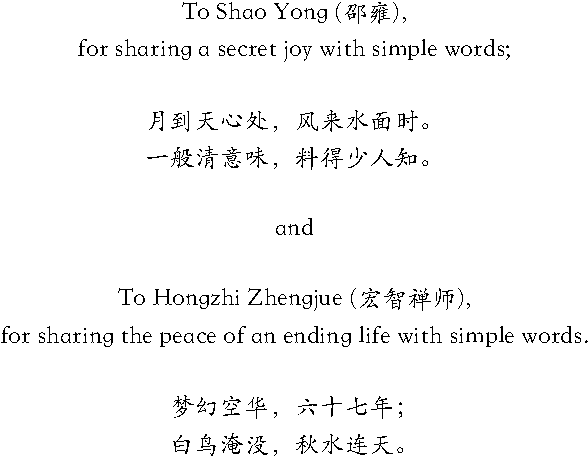
\includegraphics{images/dedication.pdf}
\end{center}

\setlength{\abovedisplayskip}{-5pt}
\setlength{\abovedisplayshortskip}{-5pt}

{
\setcounter{tocdepth}{1}
\tableofcontents
}
\hypertarget{prefuxe1cio}{%
\chapter*{Prefácio}\label{prefuxe1cio}}
\addcontentsline{toc}{chapter}{Prefácio}

Esta página serviu para estudo e prática com o pacote R Bookdown e contém a solução encontrada por mim para os exercícios propostos no livro R para Data Sciente, de Hadley Wickham e Garret Grolemund, publicado no Brasil em 2019 pela Alta Books Editora \citep{wickham2019}.

Por se tratar de um produto construído durante o processo de aprendizagem, o conteúdo pode conter erros, tanto no texto em si, como na lógica utilizada para solução dos exercícios.

Dúvidas ou sugestões de melhoria podem ser encaminhadas para o e-mail \emph{\href{mailto:jeidsan.pereira@gmail.com}{\nolinkurl{jeidsan.pereira@gmail.com}}}.

\hypertarget{penduxeancias}{%
\section*{Pendências}\label{penduxeancias}}
\addcontentsline{toc}{section}{Pendências}

\begin{itemize}
\tightlist
\item
  No PDF, o prefácio está sendo exibido duas vezes no sumário;
\item
  \protect\hyperlink{exr1-7-4}{Exercício 1.7.4};
\item
  \protect\hyperlink{exr2-3-3}{Exercício 2.3.3};
\item
  \protect\hyperlink{exr3-5-1}{Exercício 3.5.1};
\item
  \protect\hyperlink{exr3-7-1}{Exercício 3.7.1};
\item
  \protect\hyperlink{exr3-8-1}{Exercício 3.8.1};
\item
  \protect\hyperlink{exr4-2-1}{Exercício 4.2.1};
\item
  \protect\hyperlink{exr4-2-2}{Exercício 4.2.2};
\item
  \protect\hyperlink{exr5-5-4}{Exercício 5.5.4};
\item
  \protect\hyperlink{exr5-5-8}{Exercício 5.5.8};
\item
  \protect\hyperlink{exr5-5-9}{Exercício 5.5.9};
\item
  \protect\hyperlink{exr5-5-12}{Exercício 5.5.12};
\item
  \protect\hyperlink{exr8-2-3}{Exercício 8.2.3};
\item
  \protect\hyperlink{exr8-3-6}{Exercício 8.3.6};
\item
  \protect\hyperlink{exr9-5-2}{Exercício 9.5.2};
\item
  \protect\hyperlink{exr10-2-1}{Exercício 10.2.1};
\item
  \protect\hyperlink{exr10-3-2}{Exercício 10.3.2};
\item
  \protect\hyperlink{exr10-3-3}{Exercício 10.3.3};
\item
  \protect\hyperlink{exr10-4-3}{Exercício 10.4.3};
\item
  Exercícios do capítulo 11;
\item
  \protect\hyperlink{exr12-3-3}{Exercício 12.3.3};
\item
  \protect\hyperlink{exr13-3-3}{Exercício 13.3.3};
\item
  \protect\hyperlink{exr13-3-7}{Exercício 13.3.7};
\item
  \protect\hyperlink{exr15-2-7}{Exercício 15.2.7};
\item
  \protect\hyperlink{exr15-3-2}{Exercício 15.3.2};
\item
  \protect\hyperlink{exr15-3-3}{Exercício 15.3.3};
\item
  \protect\hyperlink{exr15-3-4}{Exercício 15.3.4};
\item
  Exercícios da seção 15.5;
\item
  \protect\hyperlink{exr16-3-3}{Exercício 16.3.3};
\item
  \protect\hyperlink{exr16-4-3}{Exercício 16.4.3};
\item
  \protect\hyperlink{exr16-4-5}{Exercício 16.4.5};
\item
  \protect\hyperlink{exr16-5-1}{Exercício 16.5.1};
\item
  \protect\hyperlink{exr17-3-1}{Exercício 17.3.1};
\item
  \protect\hyperlink{exr17-4-1}{Exercício 17.4.1};
\item
  \protect\hyperlink{exr17-4-1}{Exercício 17.4.1};
\item
  Exercícios da seção 17.5;
\item
  Exercícios da seção 17.9;
\item
\end{itemize}

\mainmatter

\hypertarget{part-explorar}{%
\part{Explorar}\label{part-explorar}}

\hypertarget{visualizauxe7uxe3o-de-dados-com-ggplot2}{%
\chapter{\texorpdfstring{Visualização de dados com \texttt{ggplot2}}{Visualização de dados com ggplot2}}\label{visualizauxe7uxe3o-de-dados-com-ggplot2}}

Para a correta execução dos códigos desse capítulo, utilizaremos algumas configurações específicas.

Inicialmente, precisaremos carregar o pacote \texttt{nycflights13}, que contém os dados de todos os voos da cidade de Nova York em 2013.

\begin{Shaded}
\begin{Highlighting}[]
\FunctionTok{library}\NormalTok{(nycflights13)}
\FunctionTok{library}\NormalTok{(gridExtra)}
\end{Highlighting}
\end{Shaded}

\begin{verbatim}
## 
## Attaching package: 'gridExtra'
\end{verbatim}

\begin{verbatim}
## The following object is masked from 'package:dplyr':
## 
##     combine
\end{verbatim}

\hypertarget{introduuxe7uxe3o}{%
\section{Introdução}\label{introduuxe7uxe3o}}

Não temos exercícios nesta seção.

\hypertarget{primeiros-passos}{%
\section{Primeiros passos}\label{primeiros-passos}}

\hypertarget{exr1-2-1}{%
\subsection*{Exercício 1.2.1}\label{exr1-2-1}}
\addcontentsline{toc}{subsection}{Exercício 1.2.1}

Execute \texttt{ggplot(data=mpg);}. O que você vê?

\begin{solution}
\leavevmode

\begin{Shaded}
\begin{Highlighting}[]
\FunctionTok{ggplot}\NormalTok{(}\AttributeTok{data=}\NormalTok{mpg) }\SpecialCharTok{+}
\NormalTok{    tema}
\end{Highlighting}
\end{Shaded}


\includegraphics{r4ds_files/figure-latex/unnamed-chunk-3-1.pdf}

É exibido um quadro em branco. Este quadro contém o sistema de coordenadas sobre o qual serão desenhados os grpaficos que pretendemos exibir.

\end{solution}

\hypertarget{exr1-2-2}{%
\subsection*{Exercício 1.2.2}\label{exr1-2-2}}
\addcontentsline{toc}{subsection}{Exercício 1.2.2}

Quantas linhas existem em \texttt{mtcars}? Quantas colunas?

\begin{solution}
\leavevmode

\begin{Shaded}
\begin{Highlighting}[]
\FunctionTok{dim}\NormalTok{(mtcars)}
\end{Highlighting}
\end{Shaded}

\begin{verbatim}
## [1] 32 11
\end{verbatim}

R.: Existem 32 linhas e 11 colunas.

\end{solution}

\hypertarget{exr1-2-3}{%
\subsection*{Exercício 1.2.3}\label{exr1-2-3}}
\addcontentsline{toc}{subsection}{Exercício 1.2.3}

O que a variável \texttt{drv} descreve?

\begin{solution}
Executamos o comando \texttt{?mpg} no console no R e a página de ajuda foi aberta. Nela encontramos o significado de cada variável do conjunto de dados.

A varíável descreve o tipo de tração dos carros analisados, onde \texttt{f} significa tração dianteira, \texttt{r} significa tração traseira e \texttt{4} significa tração nas quatro rodas.
\end{solution}

\hypertarget{ex1-2-4}{%
\subsection*{Exercício 1.2.4}\label{ex1-2-4}}
\addcontentsline{toc}{subsection}{Exercício 1.2.4}

Faça um gráfico de dispersão de \texttt{hwy} \emph{versus} \texttt{cyl}.

\begin{solution}
\leavevmode

\begin{Shaded}
\begin{Highlighting}[]
\FunctionTok{ggplot}\NormalTok{(}\AttributeTok{data =}\NormalTok{ mpg) }\SpecialCharTok{+}
    \FunctionTok{geom\_point}\NormalTok{(}\AttributeTok{mapping =} \FunctionTok{aes}\NormalTok{(}\AttributeTok{x =}\NormalTok{ hwy, }\AttributeTok{y =}\NormalTok{ cyl)) }\SpecialCharTok{+}
\NormalTok{    tema}
\end{Highlighting}
\end{Shaded}

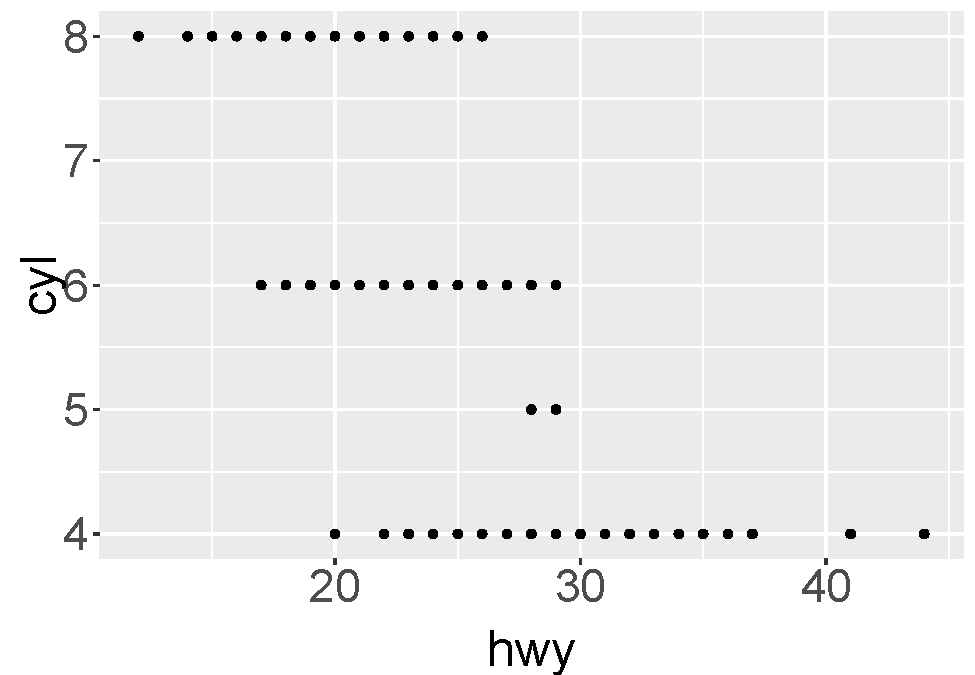
\includegraphics{r4ds_files/figure-latex/unnamed-chunk-5-1.pdf}

\end{solution}

\hypertarget{exr1-2-5}{%
\subsection*{Exercício 1.2.5}\label{exr1-2-5}}
\addcontentsline{toc}{subsection}{Exercício 1.2.5}

O que acontece se você fizer um gráfico de dispersão de \texttt{class} \emph{versus} \texttt{drv}? Por que esse gráfico não é útil?

\begin{solution}
\leavevmode

\begin{Shaded}
\begin{Highlighting}[]
\FunctionTok{ggplot}\NormalTok{(}\AttributeTok{data =}\NormalTok{ mpg) }\SpecialCharTok{+}
    \FunctionTok{geom\_point}\NormalTok{(}\AttributeTok{mapping =} \FunctionTok{aes}\NormalTok{(}\AttributeTok{x =}\NormalTok{ drv, }\AttributeTok{y =}\NormalTok{ class)) }\SpecialCharTok{+}
\NormalTok{    tema}
\end{Highlighting}
\end{Shaded}

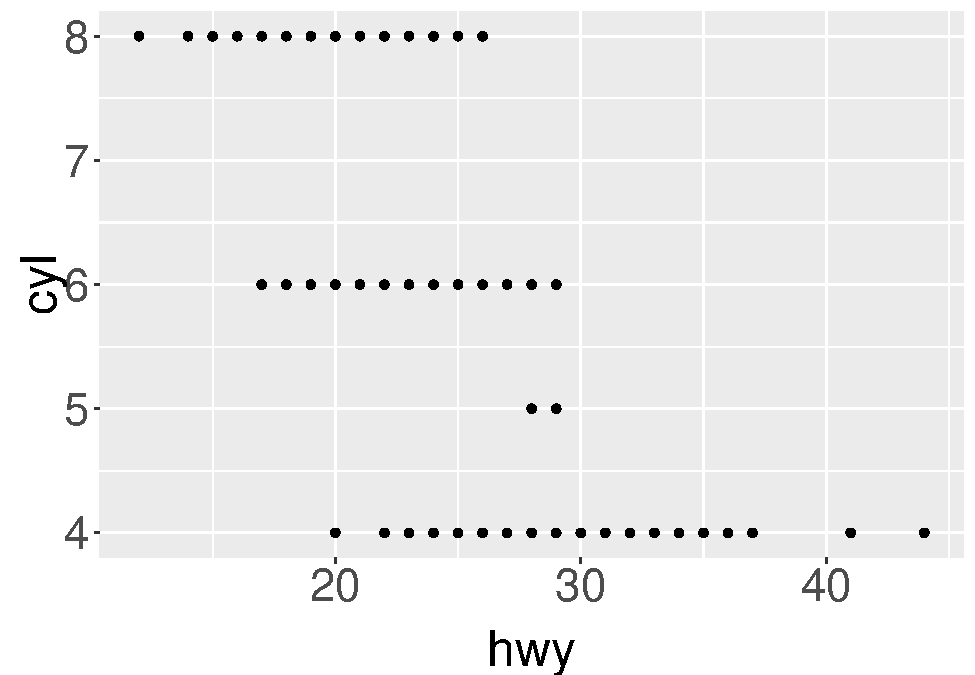
\includegraphics{r4ds_files/figure-latex/unnamed-chunk-6-1.pdf}

Apesar de serem exibidos dados no gráfico, nenhuma informação substancial é extraída, uma vez que o tipo de tração não está (a princípio) relacionado com a categoria do carro. Outro fator que torno o gráfico pouco informativo é que há, por exemplo, diversas SUVs com tração nas 4 rodas, contudo os valores ficam sobrepostos no gráfico, não dando dimensão do quanto de dados temos.

Abaixo seguem duas opções de como trazer mais informação ao gráfico:

\begin{itemize}
\tightlist
\item
  a primeira opção adiciona um ruído aos dados (\texttt{position\ =\ jitter} ou \texttt{geom\_jitter()}) de modo que não haja sobreposição;
\end{itemize}

\begin{Shaded}
\begin{Highlighting}[]
\FunctionTok{ggplot}\NormalTok{(}\AttributeTok{data =}\NormalTok{ mpg) }\SpecialCharTok{+}
    \FunctionTok{geom\_point}\NormalTok{(}\AttributeTok{mapping =} \FunctionTok{aes}\NormalTok{(}\AttributeTok{x =}\NormalTok{ drv, }\AttributeTok{y =}\NormalTok{ class), }\AttributeTok{position =} \StringTok{"jitter"}\NormalTok{) }\SpecialCharTok{+}
\NormalTok{    tema}
\end{Highlighting}
\end{Shaded}

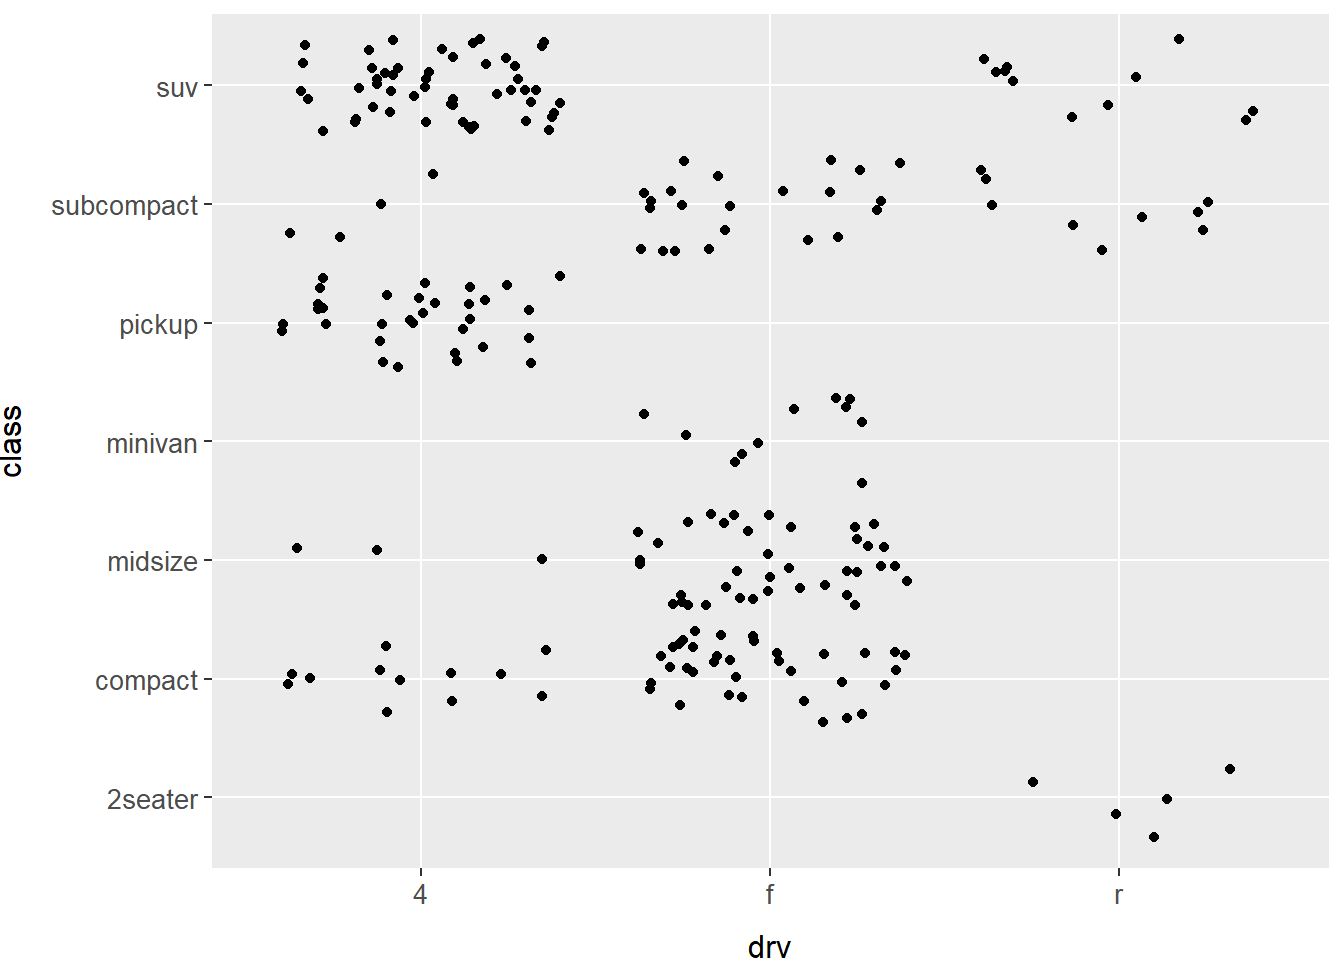
\includegraphics{r4ds_files/figure-latex/unnamed-chunk-7-1.pdf}

\begin{itemize}
\tightlist
\item
  a segunda opção, bem mais avançada, adiciona uma estética de \texttt{size} considerando a quantidade de registros.
\end{itemize}

\begin{Shaded}
\begin{Highlighting}[]
\NormalTok{mpg }\SpecialCharTok{\%\textgreater{}\%}
    \FunctionTok{group\_by}\NormalTok{(class, drv) }\SpecialCharTok{\%\textgreater{}\%}
    \FunctionTok{summarize}\NormalTok{(}\AttributeTok{count =} \FunctionTok{n}\NormalTok{()) }\SpecialCharTok{\%\textgreater{}\%}
    \FunctionTok{ggplot}\NormalTok{(}\AttributeTok{mapping =} \FunctionTok{aes}\NormalTok{(}\AttributeTok{x =}\NormalTok{ drv, }\AttributeTok{y =}\NormalTok{ class, }\AttributeTok{size =}\NormalTok{ count)) }\SpecialCharTok{+}
        \FunctionTok{geom\_point}\NormalTok{() }\SpecialCharTok{+}
\NormalTok{        tema}
\end{Highlighting}
\end{Shaded}

\begin{verbatim}
## `summarise()` has grouped output by 'class'. You can override using the
## `.groups` argument.
\end{verbatim}

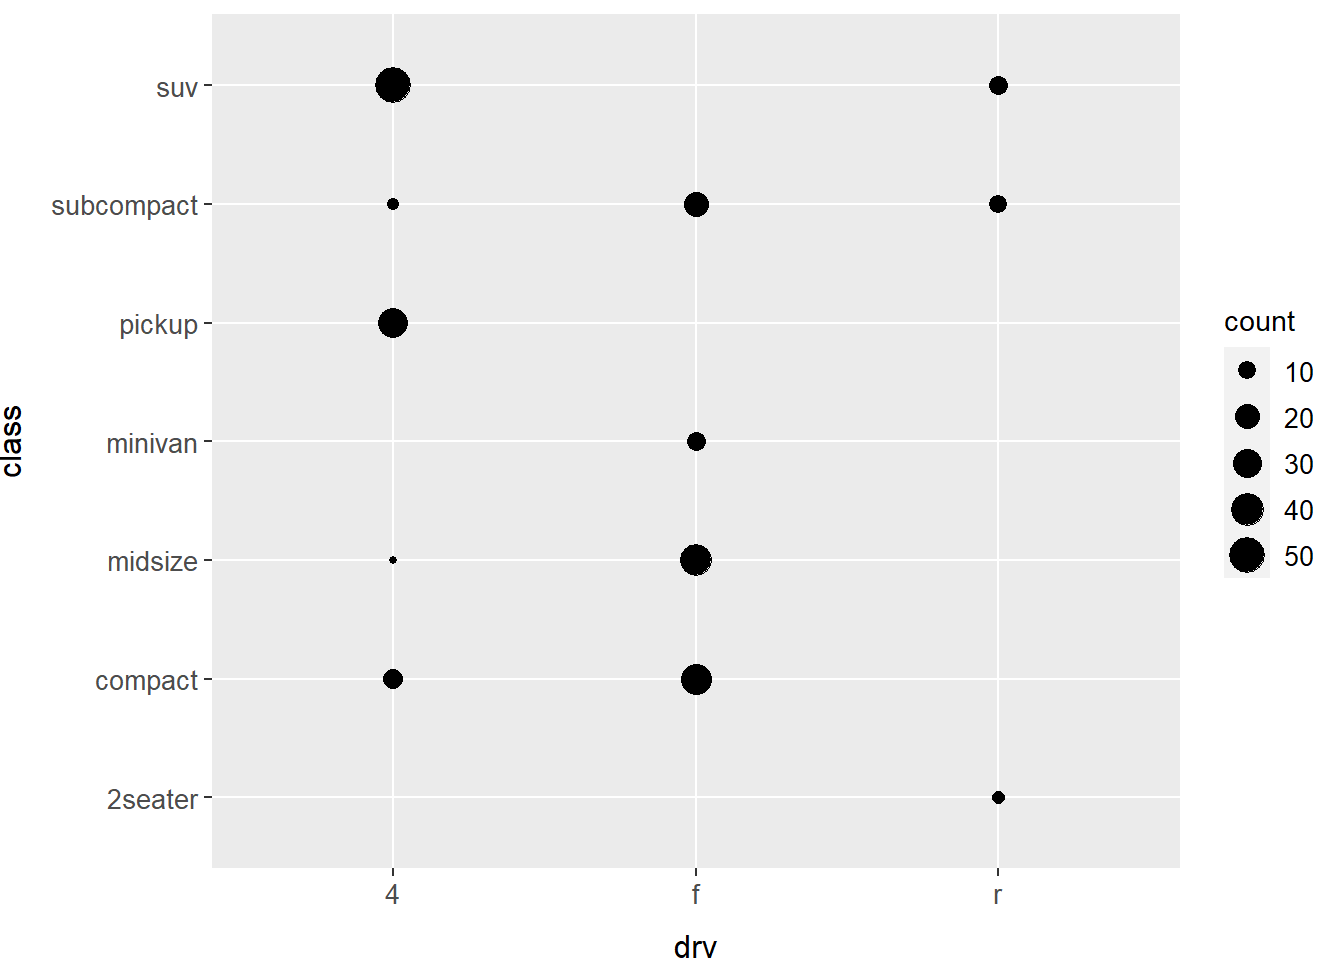
\includegraphics{r4ds_files/figure-latex/unnamed-chunk-8-1.pdf}

\end{solution}

\hypertarget{mapeamentos-estuxe9ticos}{%
\section{Mapeamentos estéticos}\label{mapeamentos-estuxe9ticos}}

\hypertarget{exr1-3-1}{%
\subsection*{Exercício 1.3.1}\label{exr1-3-1}}
\addcontentsline{toc}{subsection}{Exercício 1.3.1}

O que há de errado com este código? Por que os pontos não estão azuis?

\begin{Shaded}
\begin{Highlighting}[]
\FunctionTok{ggplot}\NormalTok{(}\AttributeTok{data =}\NormalTok{ mpg) }\SpecialCharTok{+}
    \FunctionTok{geom\_point}\NormalTok{(}\AttributeTok{mapping =} \FunctionTok{aes}\NormalTok{(}\AttributeTok{x =}\NormalTok{ displ, }\AttributeTok{y =}\NormalTok{ hwy, }\AttributeTok{color =} \StringTok{"blue"}\NormalTok{)) }\SpecialCharTok{+}
\NormalTok{    tema}
\end{Highlighting}
\end{Shaded}

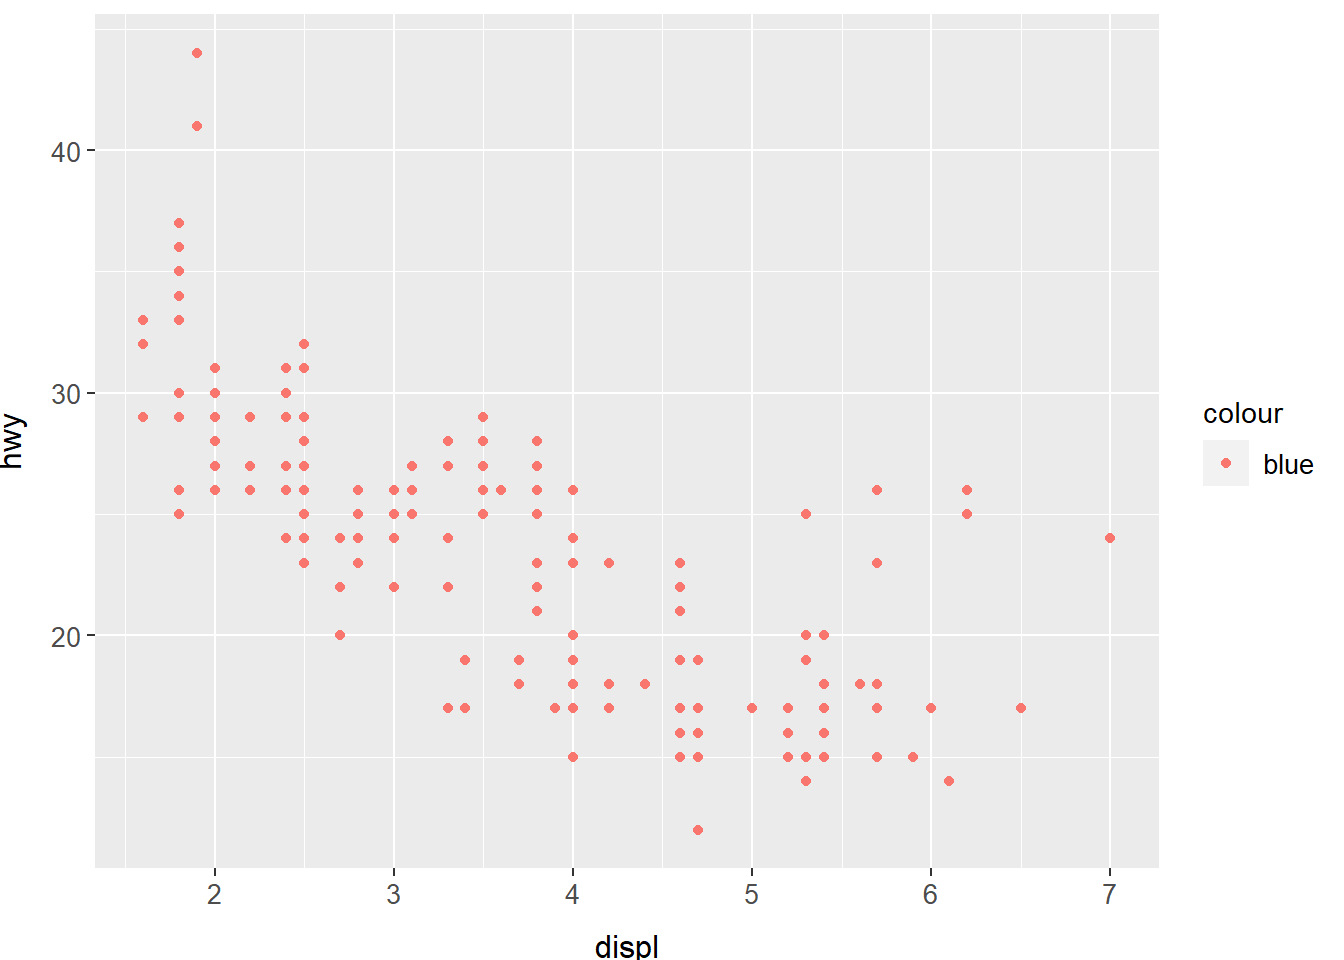
\includegraphics{r4ds_files/figure-latex/unnamed-chunk-9-1.pdf}

\begin{solution}
Ao invés de atribuir uma cor aos elementos de \texttt{geom\_point}, o atributo \texttt{color} foi passado como uma estética. O gráfico deveria ser construído da seguinte maneira:

\begin{Shaded}
\begin{Highlighting}[]
\FunctionTok{ggplot}\NormalTok{(}\AttributeTok{data =}\NormalTok{ mpg) }\SpecialCharTok{+}
    \FunctionTok{geom\_point}\NormalTok{(}\AttributeTok{mapping =} \FunctionTok{aes}\NormalTok{(}\AttributeTok{x =}\NormalTok{ displ, }\AttributeTok{y =}\NormalTok{ hwy), }\AttributeTok{color =} \StringTok{"blue"}\NormalTok{) }\SpecialCharTok{+}
\NormalTok{    tema}
\end{Highlighting}
\end{Shaded}

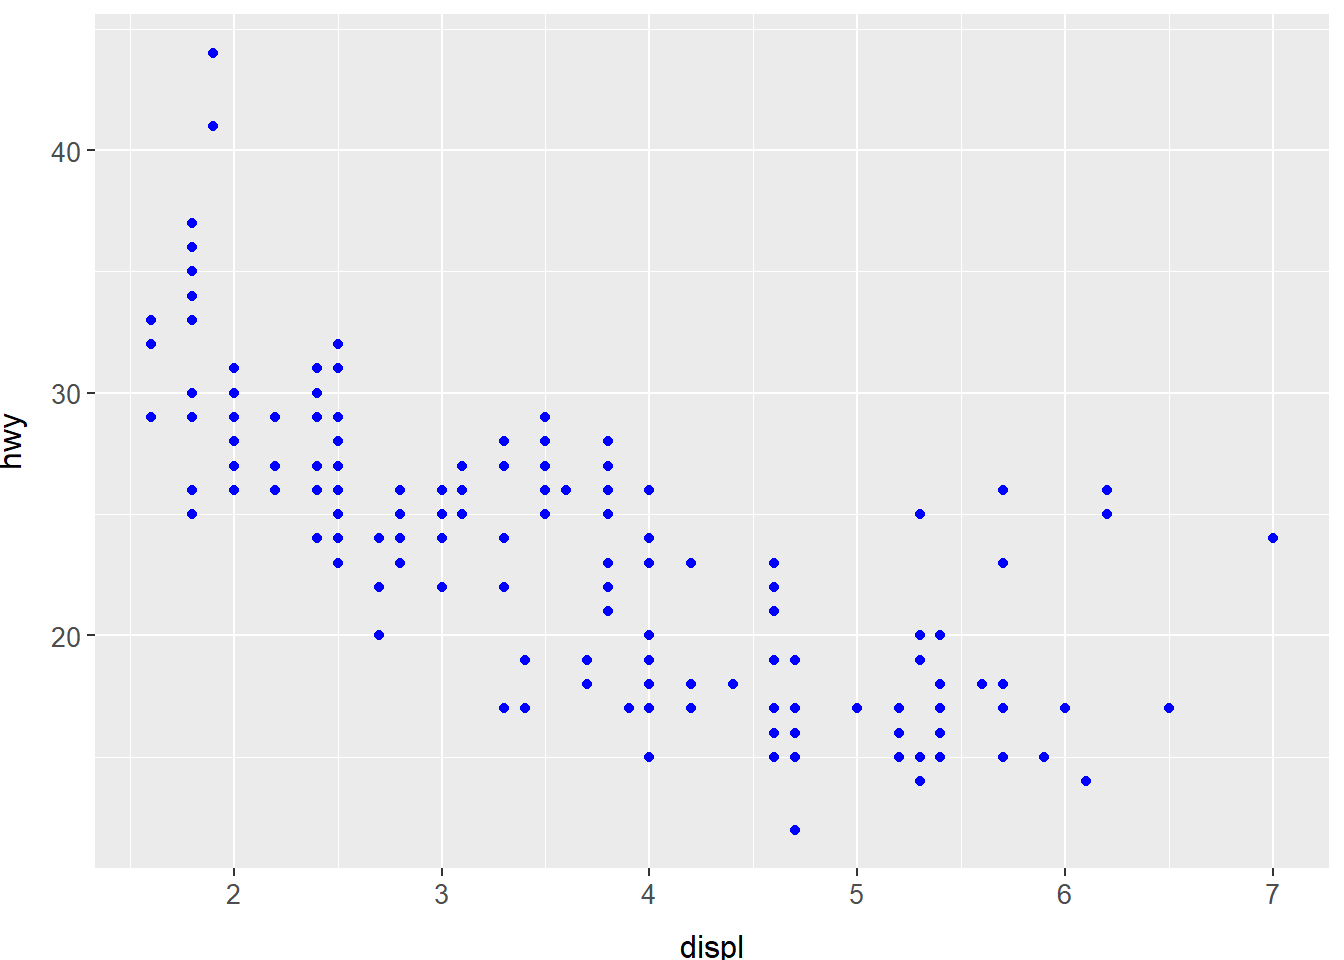
\includegraphics{r4ds_files/figure-latex/unnamed-chunk-10-1.pdf}
\end{solution}

\hypertarget{exr1-3-2}{%
\subsection*{Exercício 1.3.2}\label{exr1-3-2}}
\addcontentsline{toc}{subsection}{Exercício 1.3.2}

Quais variáveis em \texttt{mpg} são categóricas? Quais variáveis são contínuas? Como você pode ver essa informação quando executa \texttt{mpg}?

\begin{solution}
Usando \texttt{?mpg} vemos que as variáveis categóricas são: \texttt{manufacturer}, \texttt{model}, \texttt{trans}, \texttt{drv}, \texttt{fl} e \texttt{class}. As variáveis contínuas são: \texttt{displ}, \texttt{cty}, \texttt{hwy}.
\end{solution}

\hypertarget{exr1-3-3}{%
\subsection*{Exercício 1.3.3}\label{exr1-3-3}}
\addcontentsline{toc}{subsection}{Exercício 1.3.3}

Mapeie uma variável contínua para \texttt{color}, \texttt{size} e \texttt{shape}. Como essas estéticas se comportam de maneira diferente para variáveis categóricas e contínuas?

\begin{solution}
\leavevmode

\begin{Shaded}
\begin{Highlighting}[]
\FunctionTok{ggplot}\NormalTok{(}\AttributeTok{data =}\NormalTok{ mpg) }\SpecialCharTok{+}
    \FunctionTok{geom\_point}\NormalTok{(}\AttributeTok{mapping =} \FunctionTok{aes}\NormalTok{(}\AttributeTok{x =}\NormalTok{ displ, }\AttributeTok{y =}\NormalTok{ hwy, }\AttributeTok{color =}\NormalTok{ displ)) }\SpecialCharTok{+}
\NormalTok{    tema}
\end{Highlighting}
\end{Shaded}

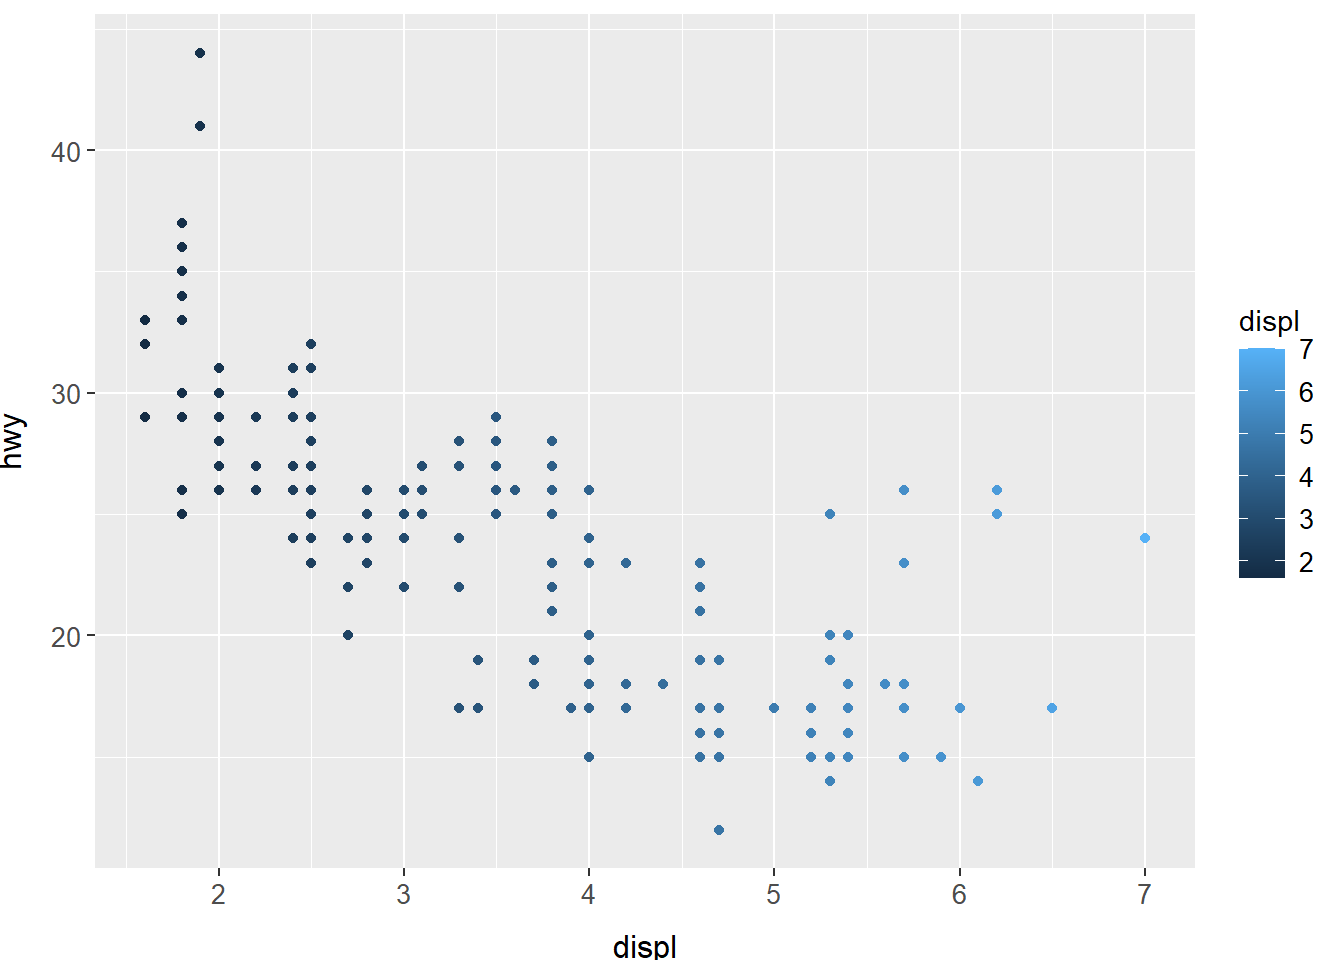
\includegraphics{r4ds_files/figure-latex/unnamed-chunk-11-1.pdf}

\begin{Shaded}
\begin{Highlighting}[]
\FunctionTok{ggplot}\NormalTok{(}\AttributeTok{data =}\NormalTok{ mpg) }\SpecialCharTok{+}
    \FunctionTok{geom\_point}\NormalTok{(}\AttributeTok{mapping =} \FunctionTok{aes}\NormalTok{(}\AttributeTok{x =}\NormalTok{ displ, }\AttributeTok{y =}\NormalTok{ hwy, }\AttributeTok{size =}\NormalTok{ displ)) }\SpecialCharTok{+}
\NormalTok{    tema}
\end{Highlighting}
\end{Shaded}

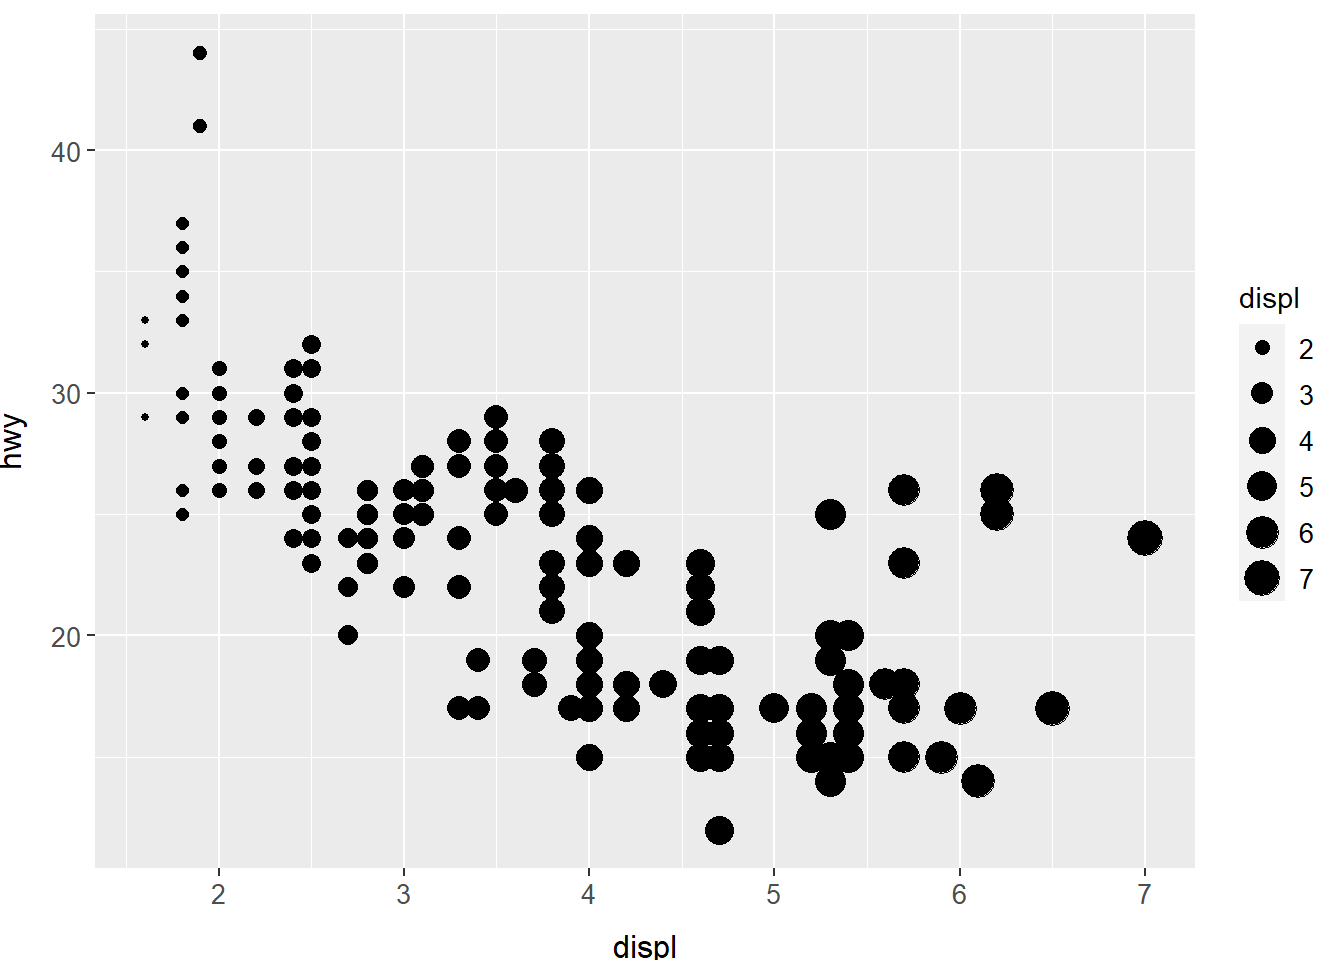
\includegraphics{r4ds_files/figure-latex/unnamed-chunk-12-1.pdf}

\begin{Shaded}
\begin{Highlighting}[]
\FunctionTok{ggplot}\NormalTok{(}\AttributeTok{data =}\NormalTok{ mpg) }\SpecialCharTok{+}
    \FunctionTok{geom\_point}\NormalTok{(}\AttributeTok{mapping =} \FunctionTok{aes}\NormalTok{(}\AttributeTok{x =}\NormalTok{ displ, }\AttributeTok{y =}\NormalTok{ hwy, }\AttributeTok{shape =}\NormalTok{ displ)) }\SpecialCharTok{+}
\NormalTok{    tema}
\end{Highlighting}
\end{Shaded}

\begin{verbatim}
## Error in `geom_point()`:
## ! Problem while computing aesthetics.
## i Error occurred in the 1st layer.
## Caused by error in `scale_f()`:
## ! A continuous variable cannot be mapped to the shape aesthetic
## i choose a different aesthetic or use `scale_shape_binned()`
\end{verbatim}

Quando possível, a biblioteca \emph{ggplot} apesenta a estética em um gradiente, como em color e size. Porém, nem sempre isso é possível, como vemos em \texttt{shape}, que só pode ser utilizada com variáveis discretas ou categóricas.

\end{solution}

\hypertarget{exr1-3-4}{%
\subsection*{Exercício 1.3.4}\label{exr1-3-4}}
\addcontentsline{toc}{subsection}{Exercício 1.3.4}

O que acontece se você mapear a mesma variável a várias estéticas?

\begin{solution}
\leavevmode

\begin{Shaded}
\begin{Highlighting}[]
\FunctionTok{ggplot}\NormalTok{(}\AttributeTok{data =}\NormalTok{ mpg) }\SpecialCharTok{+}
    \FunctionTok{geom\_point}\NormalTok{(}\AttributeTok{mapping =} \FunctionTok{aes}\NormalTok{(}\AttributeTok{x =}\NormalTok{ displ, }\AttributeTok{y =}\NormalTok{ hwy, }\AttributeTok{size =}\NormalTok{ class, }\AttributeTok{color =}\NormalTok{ class, }\AttributeTok{shape =}\NormalTok{ class)) }\SpecialCharTok{+}
\NormalTok{    tema}
\end{Highlighting}
\end{Shaded}

\begin{verbatim}
## Warning: Using size for a discrete variable is not advised.
\end{verbatim}

\begin{verbatim}
## Warning: The shape palette can deal with a maximum of 6 discrete values because
## more than 6 becomes difficult to discriminate; you have 7. Consider
## specifying shapes manually if you must have them.
\end{verbatim}

\begin{verbatim}
## Warning: Removed 62 rows containing missing values (`geom_point()`).
\end{verbatim}

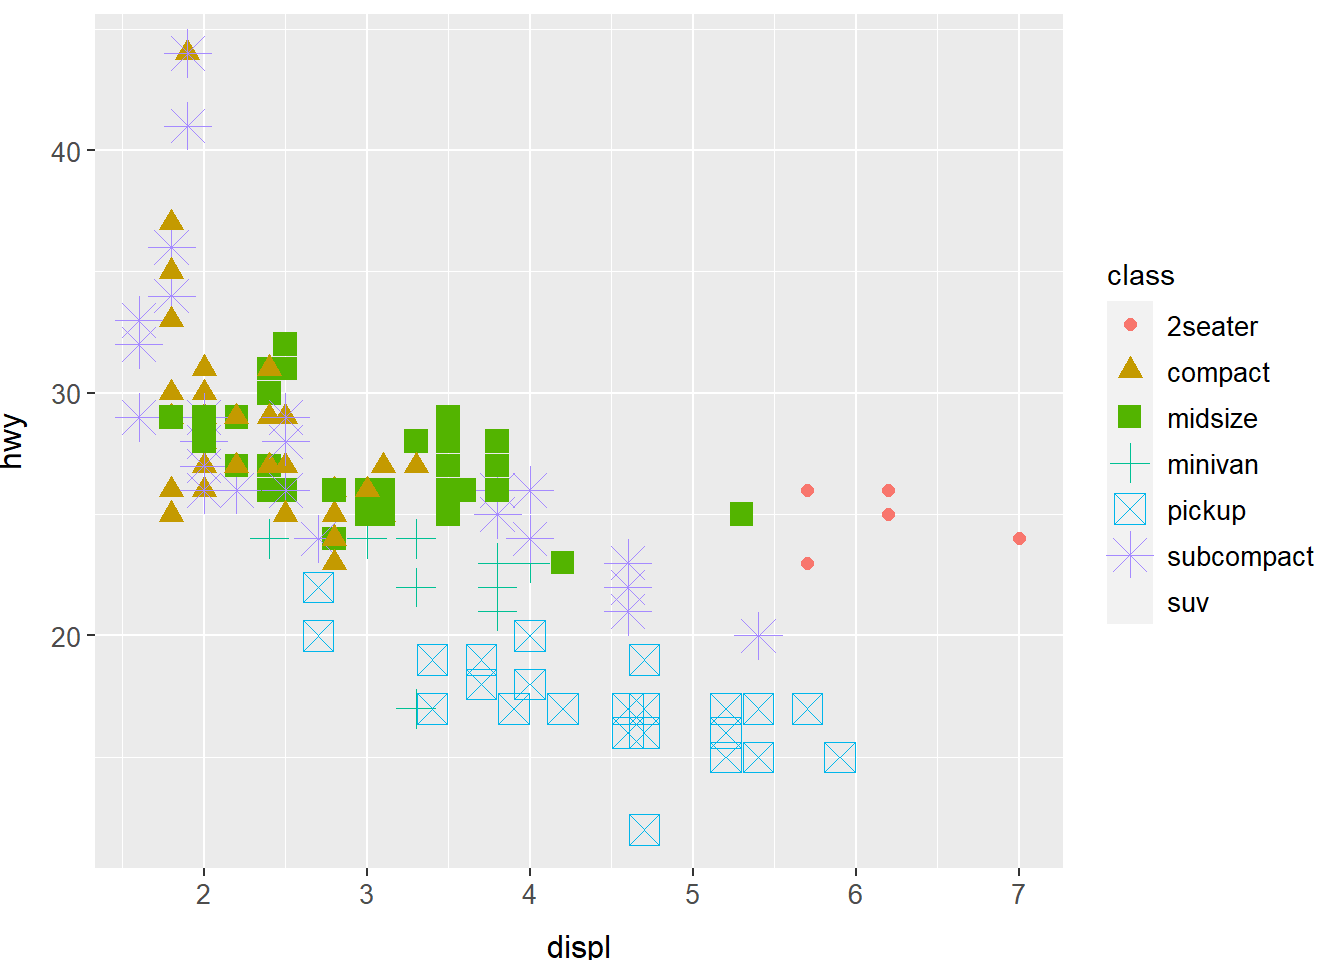
\includegraphics{r4ds_files/figure-latex/unnamed-chunk-14-1.pdf}

Os valores da variável serão representados de modo a atender todas as estéticas simultaneamente, por exemplo, no gráfico acima é dada uma cor, um formato e um tamanho específicos para cada classe de veículo. Os veículos de dois lugares são exibidos como um disco rosa pequeno.

\end{solution}

\hypertarget{exr1-3-5}{%
\subsection*{Exercício 1.3.5}\label{exr1-3-5}}
\addcontentsline{toc}{subsection}{Exercício 1.3.5}

O que a estética \texttt{stroke} faz? com que formas ela trabalha?

\begin{solution}
\leavevmode

\begin{Shaded}
\begin{Highlighting}[]
\FunctionTok{ggplot}\NormalTok{(}\AttributeTok{data =}\NormalTok{ mpg) }\SpecialCharTok{+}
    \FunctionTok{geom\_point}\NormalTok{(}\AttributeTok{mapping =} \FunctionTok{aes}\NormalTok{(}\AttributeTok{x =}\NormalTok{ displ, }\AttributeTok{y =}\NormalTok{ hwy, }\AttributeTok{stroke =}\NormalTok{ displ)) }\SpecialCharTok{+}
\NormalTok{    tema}
\end{Highlighting}
\end{Shaded}

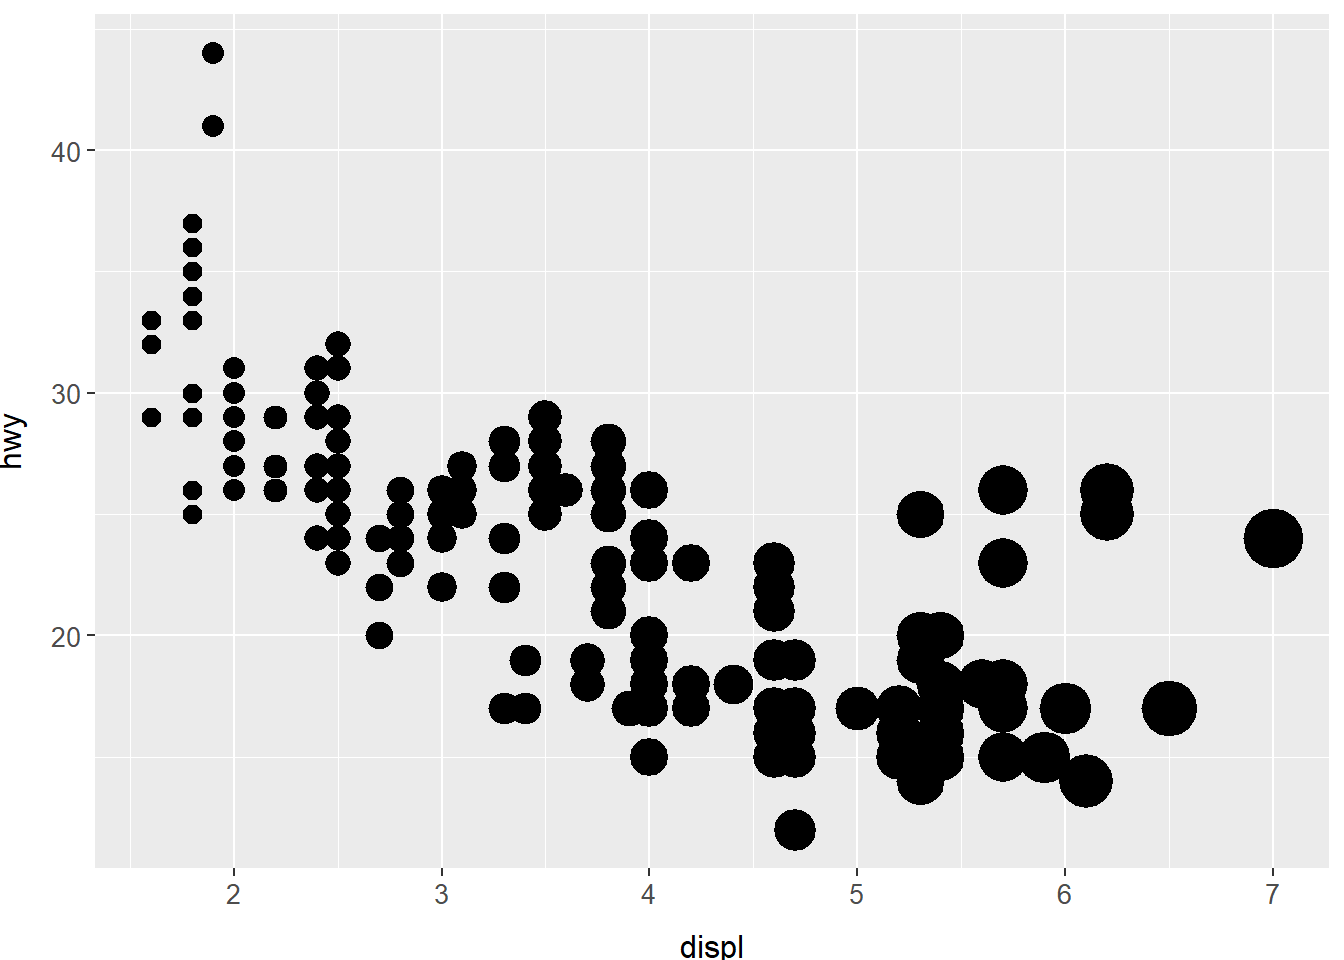
\includegraphics{r4ds_files/figure-latex/unnamed-chunk-15-1.pdf}

A estética \texttt{stroke} controla a espessura do ponto ou elemento a ser representado.

\end{solution}

\hypertarget{exr1-3-6}{%
\subsection*{Exercício 1.3.6}\label{exr1-3-6}}
\addcontentsline{toc}{subsection}{Exercício 1.3.6}

O que acontece se você mapear uma estética a algo diferente de um nome de variável, como \texttt{aes(color\ =\ displ\ \textless{}\ 5)}?

\begin{solution}
\leavevmode

\begin{Shaded}
\begin{Highlighting}[]
\FunctionTok{ggplot}\NormalTok{(}\AttributeTok{data =}\NormalTok{ mpg) }\SpecialCharTok{+}
    \FunctionTok{geom\_point}\NormalTok{(}\AttributeTok{mapping =} \FunctionTok{aes}\NormalTok{(}\AttributeTok{x =}\NormalTok{ displ, }\AttributeTok{y =}\NormalTok{ hwy, }\AttributeTok{color =}\NormalTok{ displ }\SpecialCharTok{\textless{}} \DecValTok{5}\NormalTok{)) }\SpecialCharTok{+}
\NormalTok{    tema}
\end{Highlighting}
\end{Shaded}

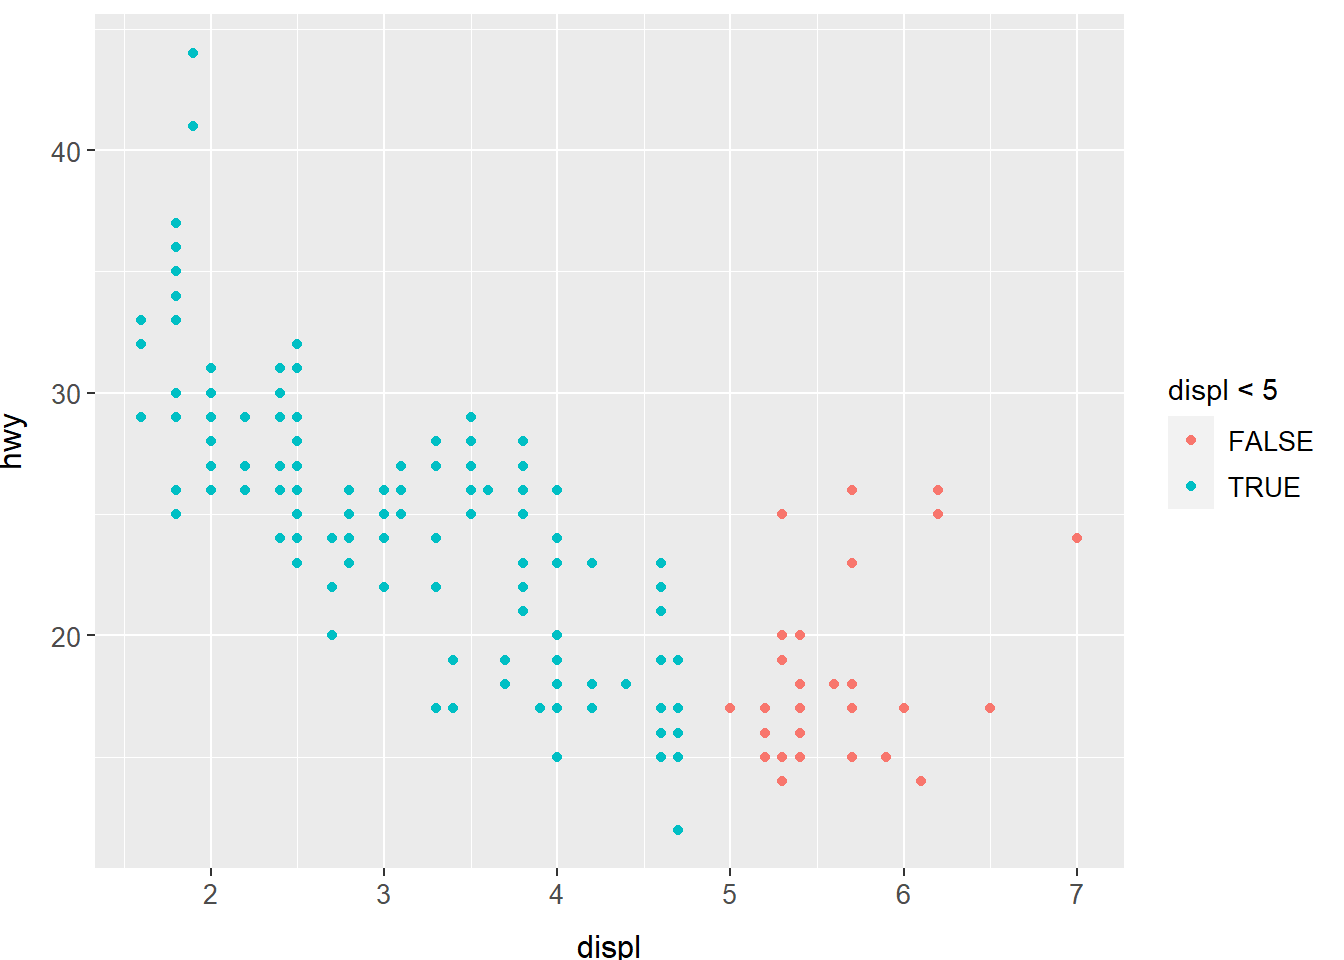
\includegraphics{r4ds_files/figure-latex/unnamed-chunk-16-1.pdf}

A expressão é avaliada para cada um dos valores da variável e o resultado é utilizado para plotagem da estética no gráfico.

\end{solution}

\hypertarget{problemas-comuns}{%
\section{Problemas comuns}\label{problemas-comuns}}

Não temos exercícios nessa seção.

\hypertarget{facetas}{%
\section{Facetas}\label{facetas}}

\hypertarget{exr1-5-1}{%
\subsection*{Exercício 1.5.1}\label{exr1-5-1}}
\addcontentsline{toc}{subsection}{Exercício 1.5.1}

O que acontece se você criar facetas em uma variável contínua?

\begin{solution}
\leavevmode

\begin{Shaded}
\begin{Highlighting}[]
\FunctionTok{ggplot}\NormalTok{(}\AttributeTok{data =}\NormalTok{ mpg) }\SpecialCharTok{+}
    \FunctionTok{geom\_point}\NormalTok{(}\AttributeTok{mapping =} \FunctionTok{aes}\NormalTok{(}\AttributeTok{x =}\NormalTok{ displ, }\AttributeTok{y =}\NormalTok{ hwy)) }\SpecialCharTok{+}
    \FunctionTok{facet\_wrap}\NormalTok{(. }\SpecialCharTok{\textasciitilde{}}\NormalTok{ displ) }\SpecialCharTok{+}
\NormalTok{    tema}
\end{Highlighting}
\end{Shaded}

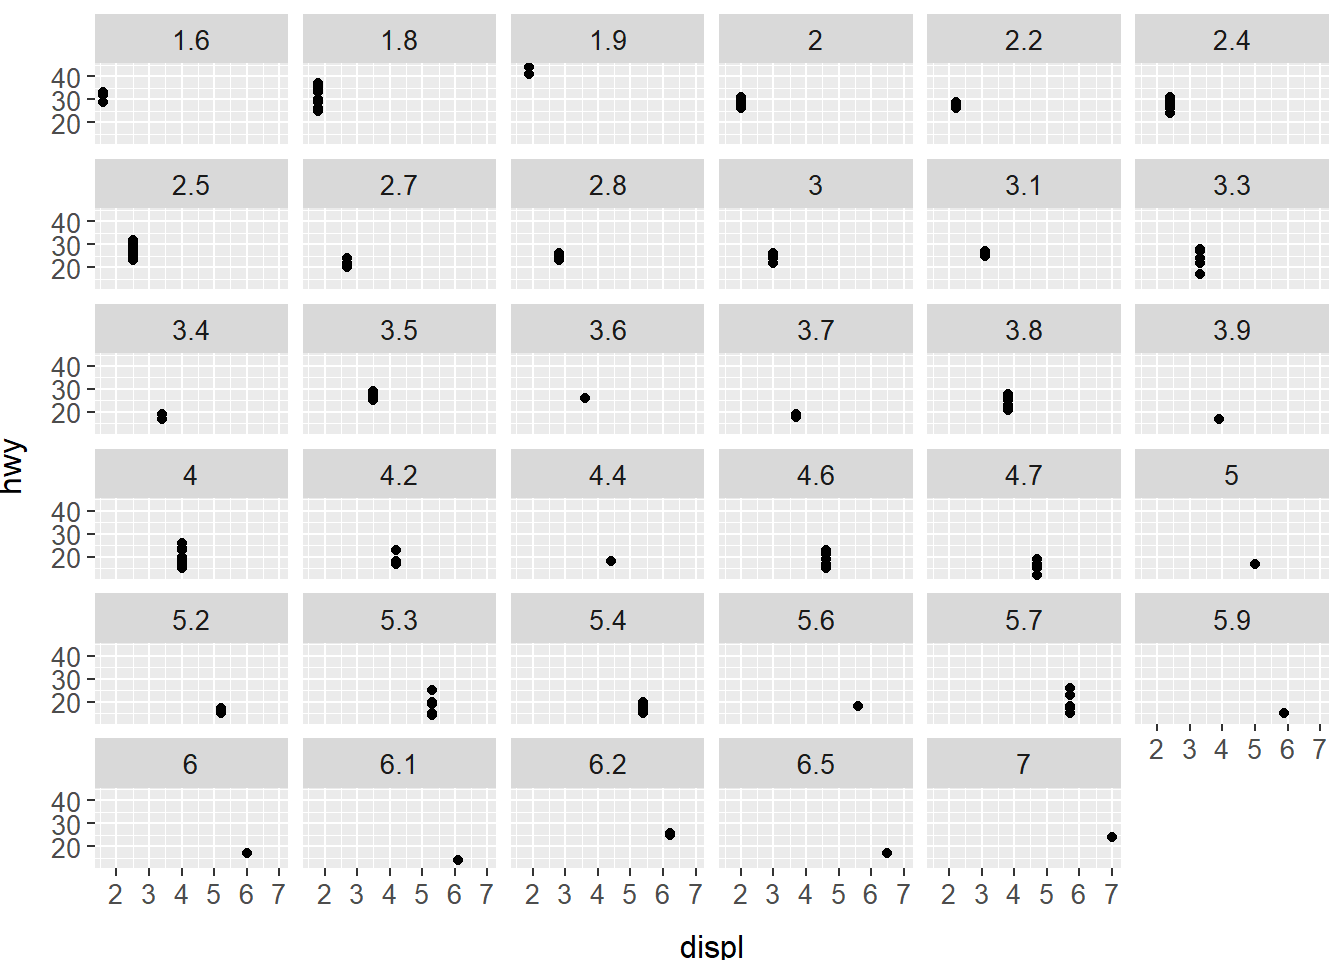
\includegraphics{r4ds_files/figure-latex/unnamed-chunk-17-1.pdf}

O \emph{ggplot} se encarrega de dividir o conjunto em classes e toma o ponto médio de cada classe para realizar a quebra em facetas.

\end{solution}

\hypertarget{exr1-5-2}{%
\subsection*{Exercício 1.5.2}\label{exr1-5-2}}
\addcontentsline{toc}{subsection}{Exercício 1.5.2}

O que significam as célula em branco em um gráfico com \texttt{facet\_grid(drv\ \textasciitilde{}\ cyl)}? Como elas se relacionam a este gráfico?

\begin{Shaded}
\begin{Highlighting}[]
\FunctionTok{ggplot}\NormalTok{(}\AttributeTok{data =}\NormalTok{ mpg) }\SpecialCharTok{+}
    \FunctionTok{geom\_point}\NormalTok{(}\AttributeTok{mapping =} \FunctionTok{aes}\NormalTok{(}\AttributeTok{x =}\NormalTok{ displ, }\AttributeTok{y =}\NormalTok{ hwy)) }\SpecialCharTok{+}
    \FunctionTok{facet\_grid}\NormalTok{(drv }\SpecialCharTok{\textasciitilde{}}\NormalTok{ cyl) }\SpecialCharTok{+}
\NormalTok{    tema}
\end{Highlighting}
\end{Shaded}

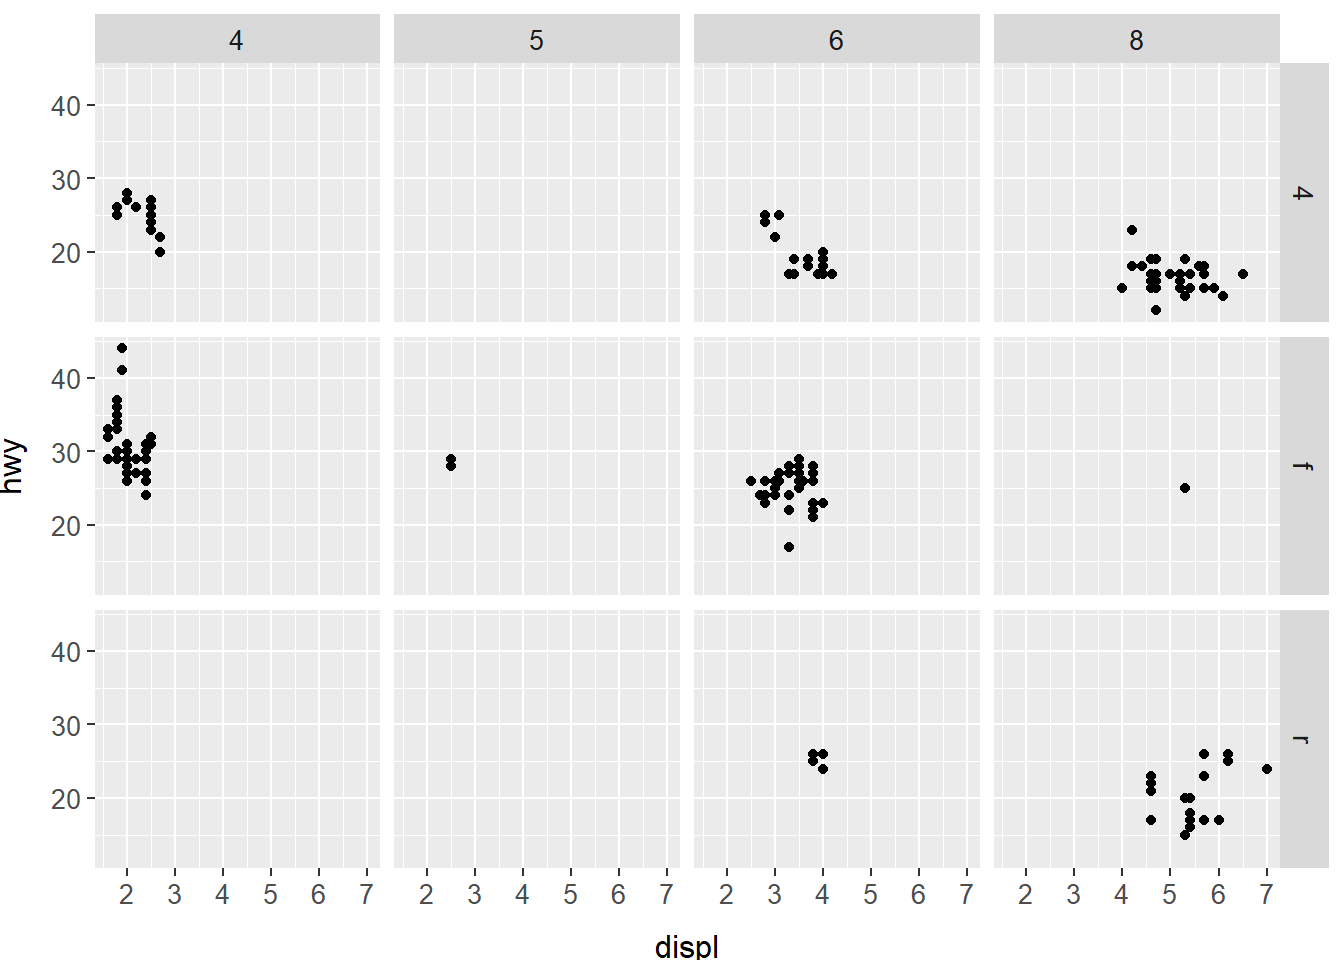
\includegraphics{r4ds_files/figure-latex/unnamed-chunk-18-1.pdf}

\begin{solution}
Significa que para aquela combinação de variáveis, não há nenhum valor observado. Por exemplo, não há nenhum veículo com 5 cilindros e tração nas quatro rodas.
\end{solution}

\hypertarget{exr1-5-3}{%
\subsection*{Exercício 1.5.3}\label{exr1-5-3}}
\addcontentsline{toc}{subsection}{Exercício 1.5.3}

Que gráficos o código a seguir faz? O que \texttt{.} faz?

\begin{Shaded}
\begin{Highlighting}[]
\FunctionTok{ggplot}\NormalTok{(}\AttributeTok{data =}\NormalTok{ mpg) }\SpecialCharTok{+}
    \FunctionTok{geom\_point}\NormalTok{(}\AttributeTok{mapping =} \FunctionTok{aes}\NormalTok{(}\AttributeTok{x =}\NormalTok{ displ, }\AttributeTok{y =}\NormalTok{ hwy)) }\SpecialCharTok{+}
    \FunctionTok{facet\_grid}\NormalTok{(drv }\SpecialCharTok{\textasciitilde{}}\NormalTok{ .) }\SpecialCharTok{+}
\NormalTok{    tema}
\end{Highlighting}
\end{Shaded}

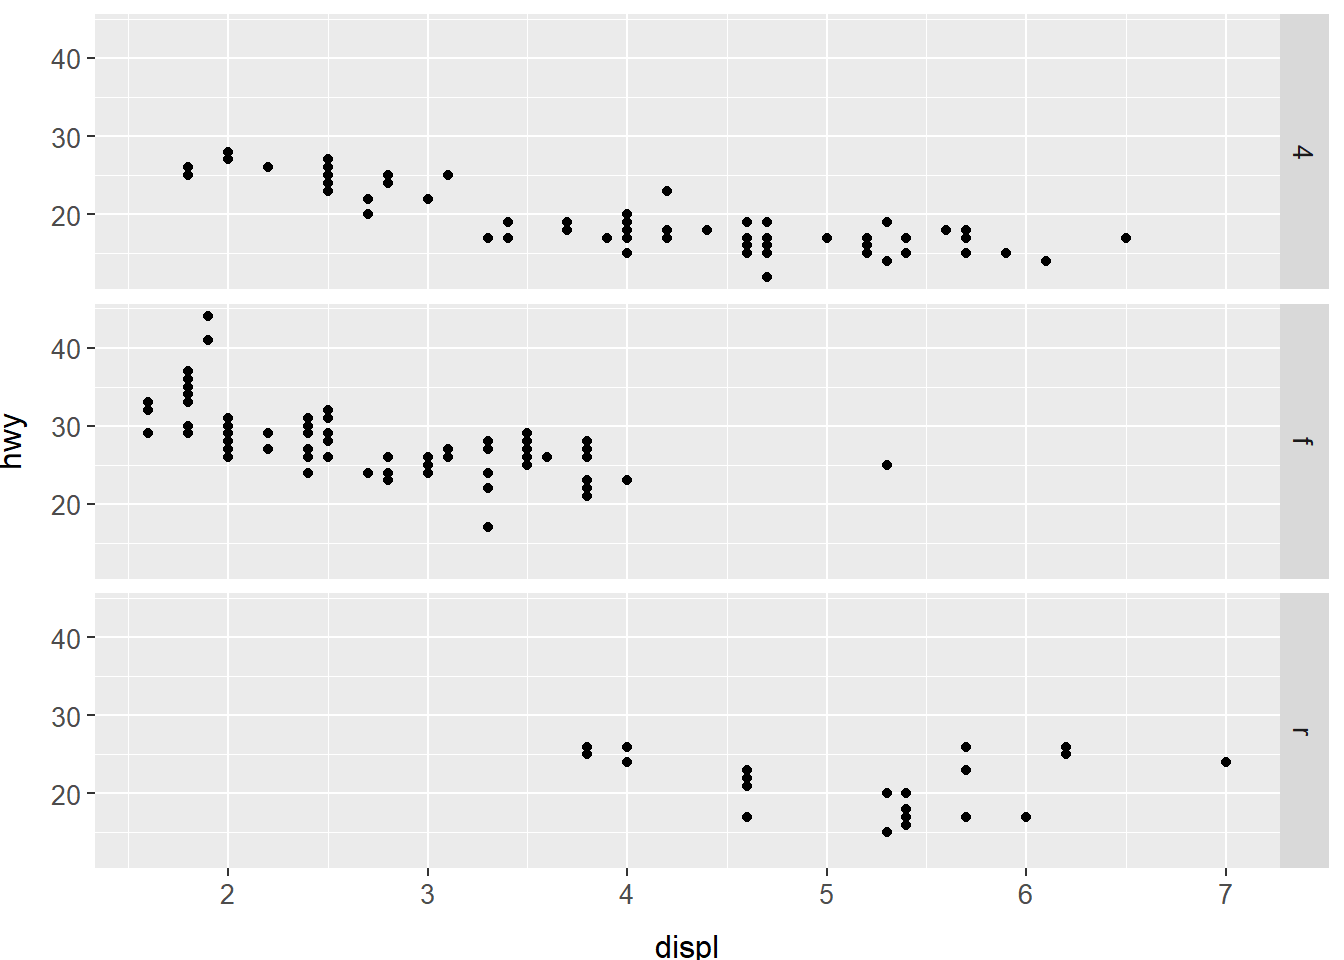
\includegraphics{r4ds_files/figure-latex/unnamed-chunk-19-1.pdf}

\begin{Shaded}
\begin{Highlighting}[]
\FunctionTok{ggplot}\NormalTok{(}\AttributeTok{data =}\NormalTok{ mpg) }\SpecialCharTok{+}
    \FunctionTok{geom\_point}\NormalTok{(}\AttributeTok{mapping =} \FunctionTok{aes}\NormalTok{(}\AttributeTok{x =}\NormalTok{ displ, }\AttributeTok{y =}\NormalTok{ hwy)) }\SpecialCharTok{+}
    \FunctionTok{facet\_grid}\NormalTok{(. }\SpecialCharTok{\textasciitilde{}}\NormalTok{ cyl) }\SpecialCharTok{+}
\NormalTok{    tema}
\end{Highlighting}
\end{Shaded}

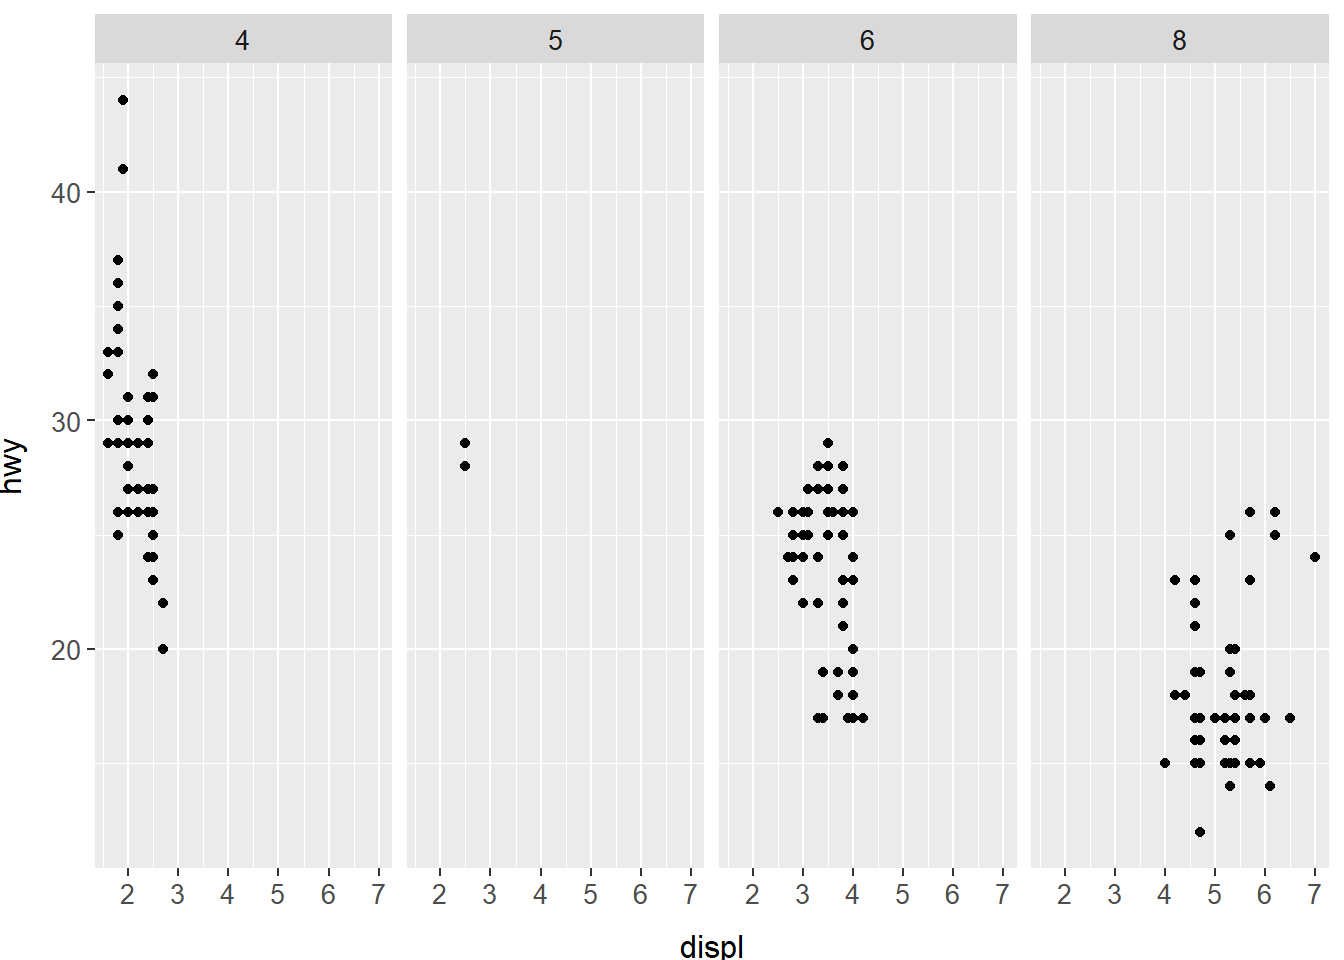
\includegraphics{r4ds_files/figure-latex/unnamed-chunk-20-1.pdf}

\begin{solution}
São gerados os gráficos de dispersão segregados pelas variáveis \texttt{drv} e \texttt{cyl}, respectivamente. O \texttt{.} indica que não queremos considerar nenhuma segregação naquela dimensão do \emph{grid} (linha ou coluna).
\end{solution}

\hypertarget{exr1-5-4}{%
\subsection*{Exercício 1.5.4}\label{exr1-5-4}}
\addcontentsline{toc}{subsection}{Exercício 1.5.4}

Pegue o primeiro gráfico em facetas dessa seção.

\begin{Shaded}
\begin{Highlighting}[]
\FunctionTok{ggplot}\NormalTok{(}\AttributeTok{data =}\NormalTok{ mpg) }\SpecialCharTok{+}
    \FunctionTok{geom\_point}\NormalTok{(}\AttributeTok{data =} \FunctionTok{transform}\NormalTok{(mpg, }\AttributeTok{class =} \ConstantTok{NULL}\NormalTok{), }\AttributeTok{mapping =} \FunctionTok{aes}\NormalTok{(}\AttributeTok{x =}\NormalTok{ displ, }\AttributeTok{y =}\NormalTok{ hwy), }\AttributeTok{color =} \StringTok{"gray80"}\NormalTok{) }\SpecialCharTok{+}
    \FunctionTok{geom\_point}\NormalTok{(}\AttributeTok{mapping =} \FunctionTok{aes}\NormalTok{(}\AttributeTok{x =}\NormalTok{ displ, }\AttributeTok{y =}\NormalTok{ hwy)) }\SpecialCharTok{+}
    \FunctionTok{facet\_wrap}\NormalTok{(}\SpecialCharTok{\textasciitilde{}}\NormalTok{ class, }\AttributeTok{nrow =} \DecValTok{2}\NormalTok{) }\SpecialCharTok{+}
\NormalTok{    tema}
\end{Highlighting}
\end{Shaded}

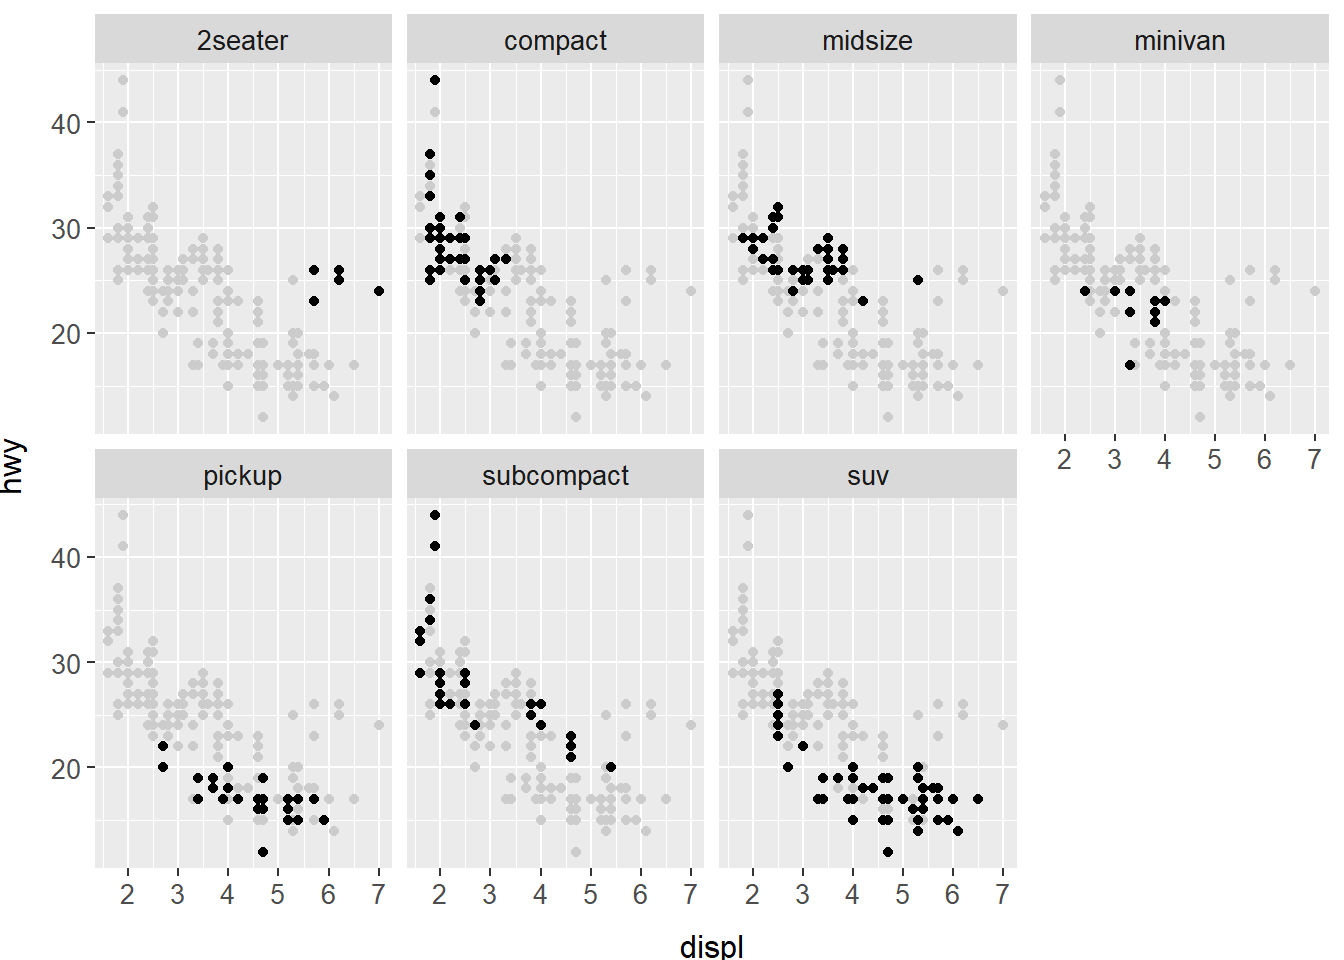
\includegraphics{r4ds_files/figure-latex/unnamed-chunk-21-1.pdf}

Quais são as vantagens de usar facetas, em vez de estética de cor? Quais são as desvantagens? Como o equilíbrio poderia mudar se você tivesse um conjunto de dados maior?

\begin{solution}
A principal vantagem no uso de facetas é que fica mais fácil analisar os dados quando eles estão separados em seu próprio contexto, contudo visualizá-los assim dificulta a comparação entre grupos.
\end{solution}

\hypertarget{exr1-5-5}{%
\subsection*{Exercício 1.5.5}\label{exr1-5-5}}
\addcontentsline{toc}{subsection}{Exercício 1.5.5}

Leia \texttt{?facet\_wrap}. O que \texttt{nrow} faz? o que \texttt{ncol} faz? Quais outras opções controlam o layout de paineis individuais? Por que \texttt{facet\_grid()} não tem variáveis \texttt{nrow}e \texttt{ncol}?

\begin{solution}
\leavevmode

\begin{verbatim}
?facet_wrap
\end{verbatim}

Os atributos \texttt{ncol} e \texttt{nrow} são utilizados pelo \texttt{facet\_wrap} para determinar o número de colunas ou linhas (respectivamente) nas quais serão distribuídos os gráficos segregados. Esses atributos não figuram em \texttt{facet\_grid} pelo fato deste já organizar as facetas retangularmente.

\end{solution}

\hypertarget{exr1-5-6}{%
\subsection*{Exercício 1.5.6}\label{exr1-5-6}}
\addcontentsline{toc}{subsection}{Exercício 1.5.6}

Ao usar \texttt{facet\_grid()} você normalmente deveria colocar a variável com níveis mais singulares nas colunas. Por quê?

\begin{solution}
Para melhor aproveitamento do espaço em tela.
\end{solution}

\hypertarget{objetos-geomuxe9tricos}{%
\section{Objetos geométricos}\label{objetos-geomuxe9tricos}}

\hypertarget{exr1-6-1}{%
\subsection*{Exercício 1.6.1}\label{exr1-6-1}}
\addcontentsline{toc}{subsection}{Exercício 1.6.1}

Que \emph{geom} você usaria para desenhar um gráfico de linha? Um diagrama de caixas (\emph{boxplot})? Um histograma? Um gráfico de área?

\begin{solution}
\leavevmode

\begin{Shaded}
\begin{Highlighting}[]
\FunctionTok{ggplot}\NormalTok{(}\AttributeTok{data =}\NormalTok{ mpg, }\AttributeTok{mapping =} \FunctionTok{aes}\NormalTok{(}\AttributeTok{x =}\NormalTok{ displ, }\AttributeTok{y =}\NormalTok{ hwy)) }\SpecialCharTok{+}
    \FunctionTok{geom\_line}\NormalTok{() }\SpecialCharTok{+}
\NormalTok{    tema}
\end{Highlighting}
\end{Shaded}

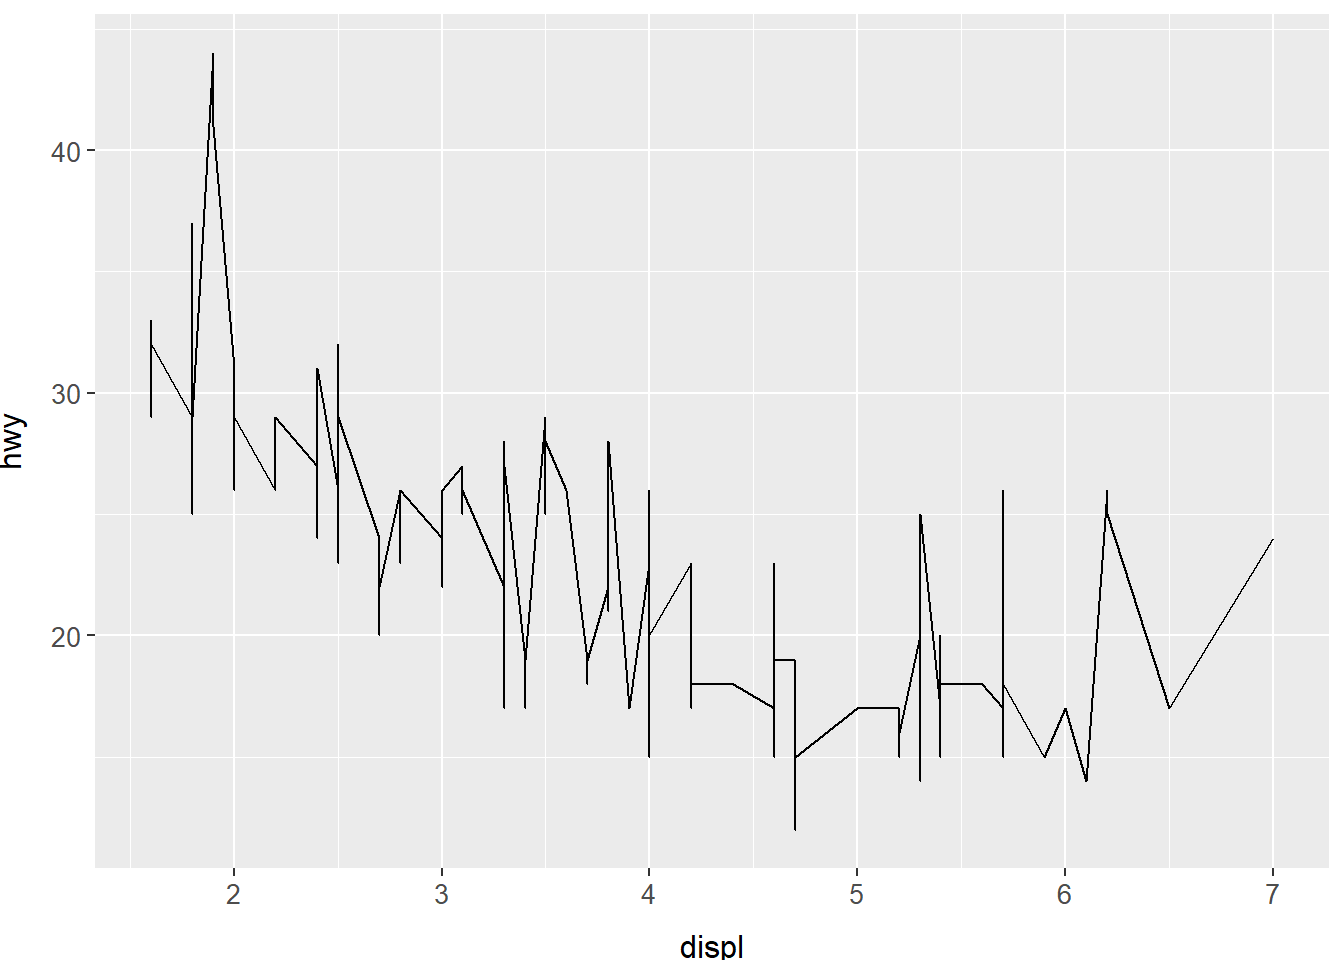
\includegraphics{r4ds_files/figure-latex/unnamed-chunk-22-1.pdf}

\begin{Shaded}
\begin{Highlighting}[]
\FunctionTok{ggplot}\NormalTok{(}\AttributeTok{data =}\NormalTok{ mpg) }\SpecialCharTok{+}
    \FunctionTok{geom\_boxplot}\NormalTok{(}\AttributeTok{mapping =} \FunctionTok{aes}\NormalTok{(}\AttributeTok{y =}\NormalTok{ hwy, }\AttributeTok{x =}\NormalTok{ class)) }\SpecialCharTok{+}
\NormalTok{    tema}
\end{Highlighting}
\end{Shaded}

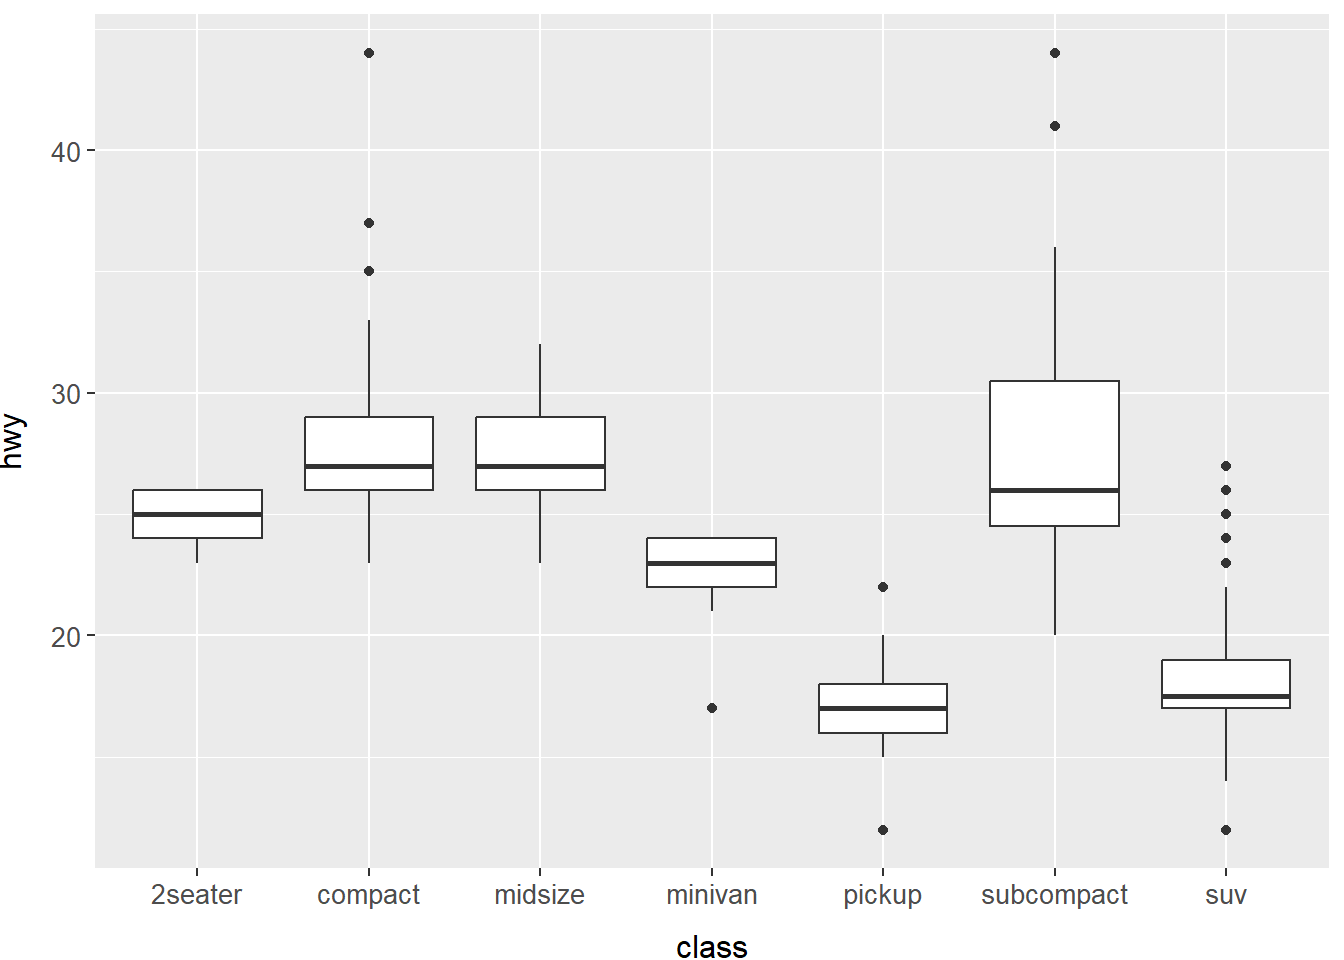
\includegraphics{r4ds_files/figure-latex/unnamed-chunk-23-1.pdf}

\begin{Shaded}
\begin{Highlighting}[]
\FunctionTok{ggplot}\NormalTok{(}\AttributeTok{data =}\NormalTok{ mpg, }\AttributeTok{mapping =} \FunctionTok{aes}\NormalTok{(}\AttributeTok{x =}\NormalTok{ hwy)) }\SpecialCharTok{+}
    \FunctionTok{geom\_histogram}\NormalTok{() }\SpecialCharTok{+}
\NormalTok{    tema}
\end{Highlighting}
\end{Shaded}

\begin{verbatim}
## `stat_bin()` using `bins = 30`. Pick better value with `binwidth`.
\end{verbatim}

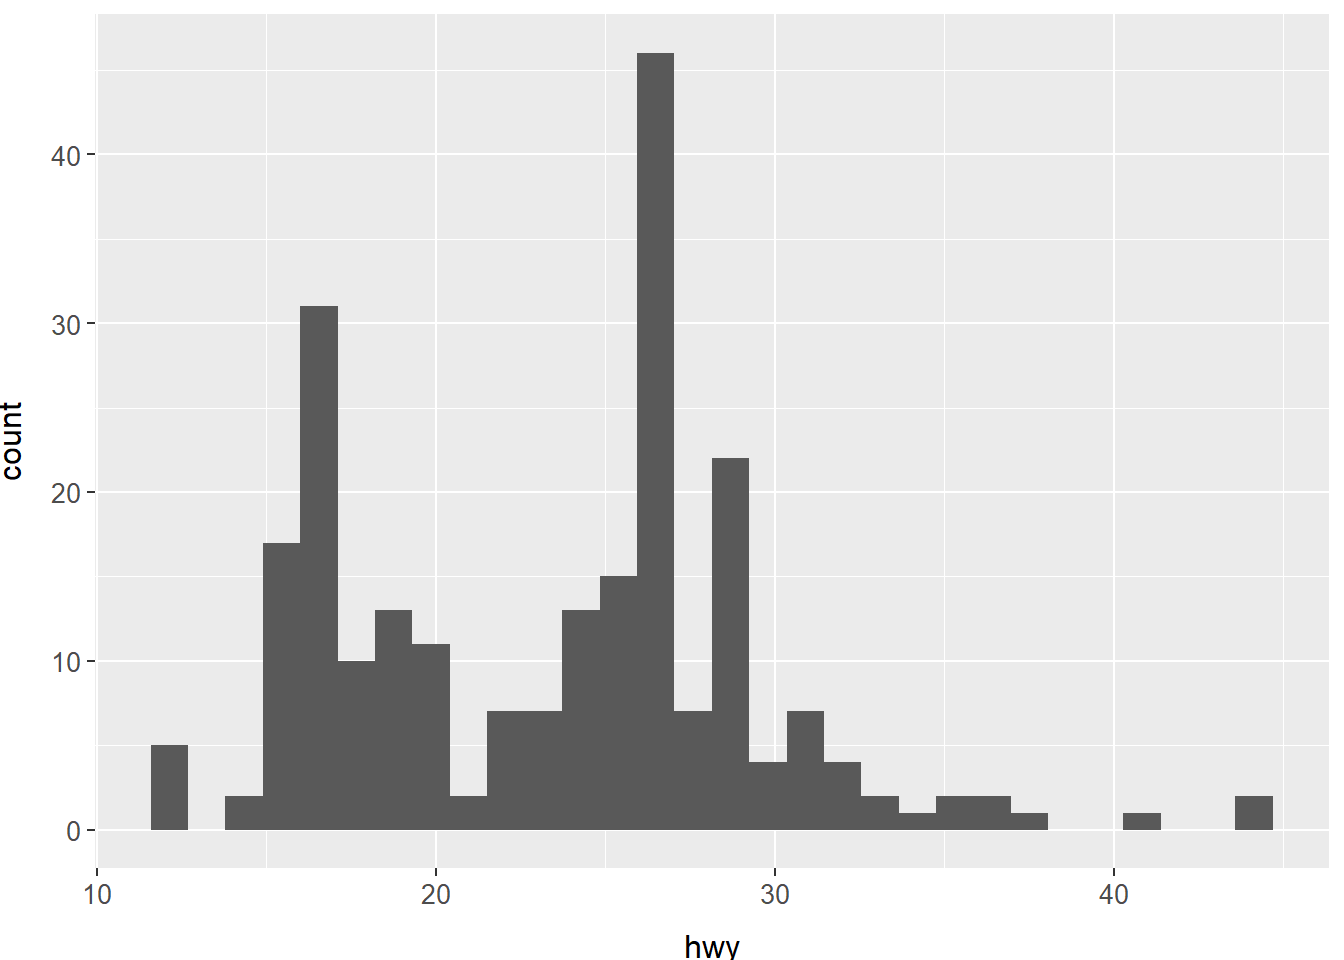
\includegraphics{r4ds_files/figure-latex/unnamed-chunk-24-1.pdf}

\begin{Shaded}
\begin{Highlighting}[]
\FunctionTok{ggplot}\NormalTok{(}\AttributeTok{data =}\NormalTok{ economics, }\AttributeTok{mapping =} \FunctionTok{aes}\NormalTok{(}\AttributeTok{x =}\NormalTok{ date, }\AttributeTok{y =}\NormalTok{ unemploy)) }\SpecialCharTok{+}
    \FunctionTok{geom\_area}\NormalTok{() }\SpecialCharTok{+}
\NormalTok{    tema}
\end{Highlighting}
\end{Shaded}

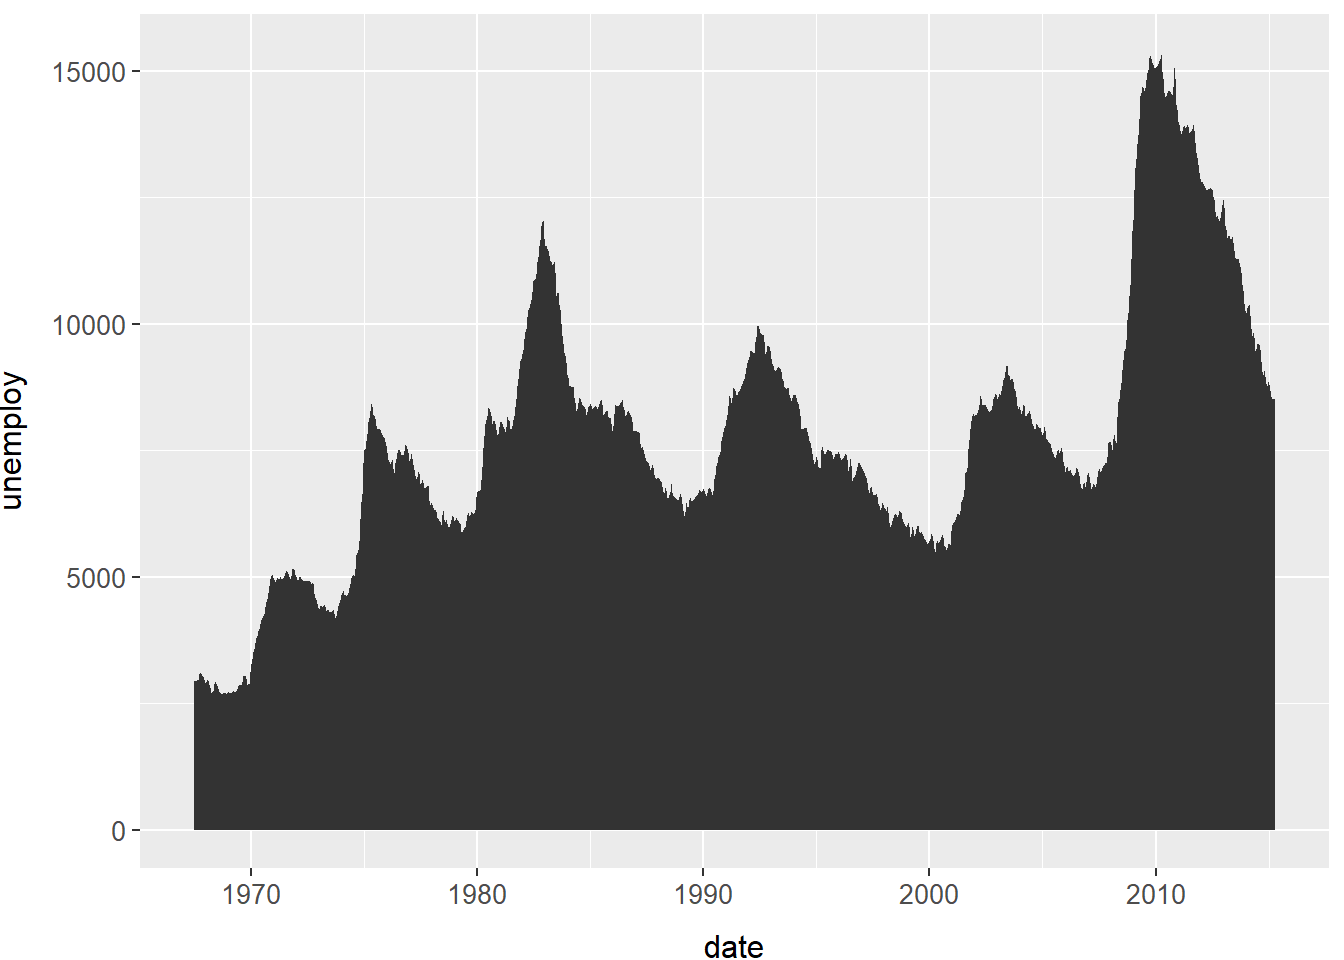
\includegraphics{r4ds_files/figure-latex/unnamed-chunk-25-1.pdf}

Podem ser utilizados, respectivamente as \emph{geoms}: \emph{line}, \emph{boxplot}, \emph{histogram} e \emph{area}.

\end{solution}

\hypertarget{exr1-6-2}{%
\subsection*{Exercício 1.6.2}\label{exr1-6-2}}
\addcontentsline{toc}{subsection}{Exercício 1.6.2}

Execute este código em sua cabeça e preveja como será o resultado. Depois execute o código no R e confira suas previsões:

\begin{Shaded}
\begin{Highlighting}[]
\FunctionTok{ggplot}\NormalTok{(}\AttributeTok{data =}\NormalTok{ mpg, }\AttributeTok{mapping =} \FunctionTok{aes}\NormalTok{(}\AttributeTok{x =}\NormalTok{ displ, }\AttributeTok{y =}\NormalTok{ hwy, }\AttributeTok{color =}\NormalTok{ drv)) }\SpecialCharTok{+}
    \FunctionTok{geom\_point}\NormalTok{() }\SpecialCharTok{+}
    \FunctionTok{geom\_smooth}\NormalTok{(}\AttributeTok{se =} \ConstantTok{FALSE}\NormalTok{) }\SpecialCharTok{+}
\NormalTok{    tema}
\end{Highlighting}
\end{Shaded}

\begin{verbatim}
## `geom_smooth()` using method = 'loess' and formula = 'y ~ x'
\end{verbatim}

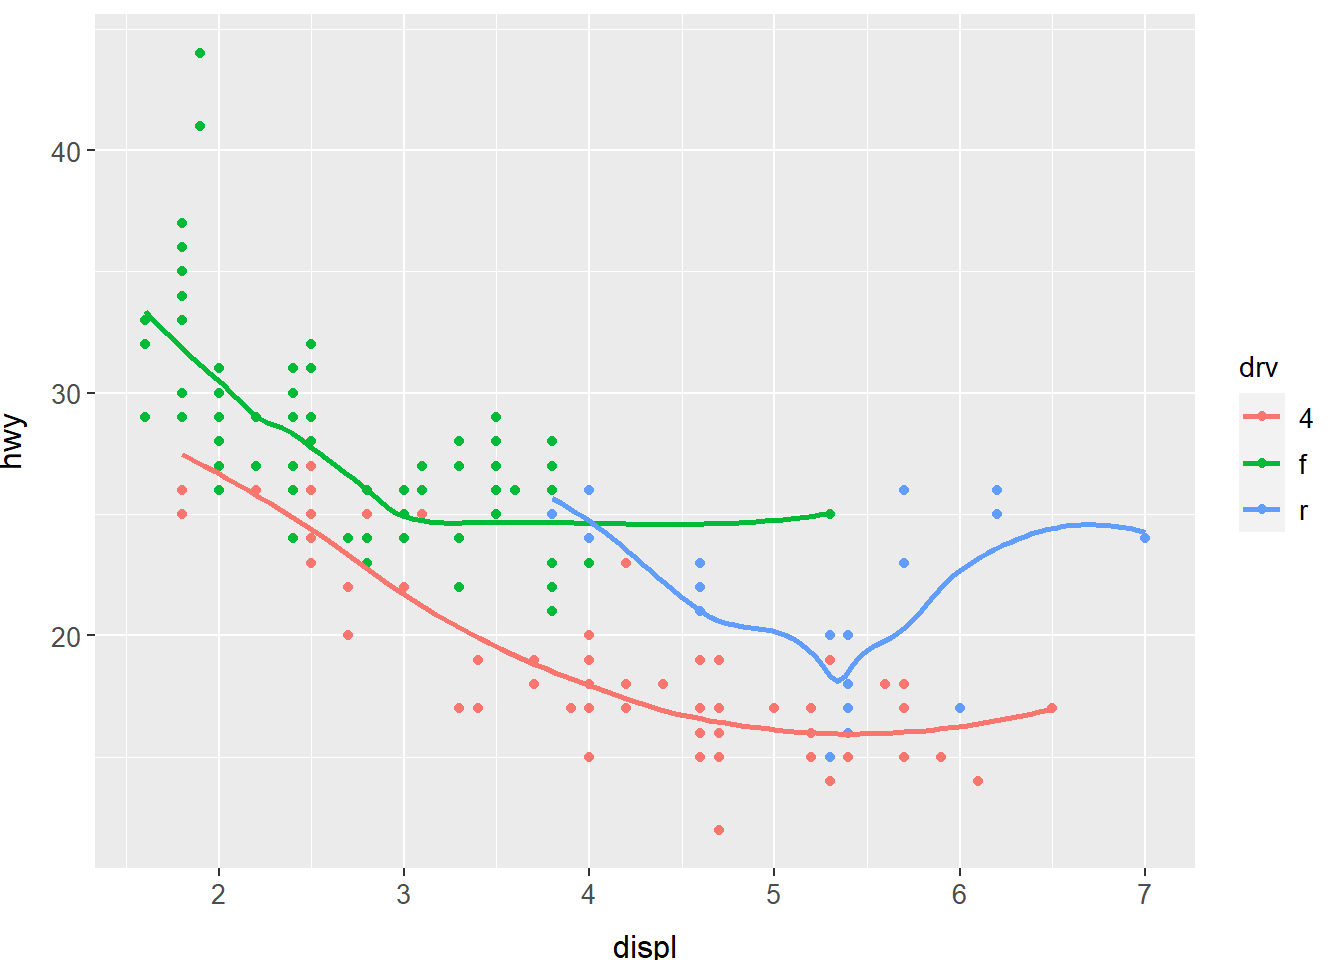
\includegraphics{r4ds_files/figure-latex/unnamed-chunk-26-1.pdf}

\begin{solution}
O gráfico bateu com a expectativa.
\end{solution}

\hypertarget{exr1-6-3}{%
\subsection*{Exercício 1.6.3}\label{exr1-6-3}}
\addcontentsline{toc}{subsection}{Exercício 1.6.3}

O que o \texttt{show.legend\ =\ FALSE} faz? O que acontece se você removê-lo? Por que você acha que usei isso anteriormente no capítulo?

\begin{solution}
\leavevmode

\begin{Shaded}
\begin{Highlighting}[]
\FunctionTok{ggplot}\NormalTok{(}\AttributeTok{data =}\NormalTok{ mpg, }\AttributeTok{mapping =} \FunctionTok{aes}\NormalTok{(}\AttributeTok{x =}\NormalTok{ displ, }\AttributeTok{y =}\NormalTok{ hwy, }\AttributeTok{color =}\NormalTok{ drv)) }\SpecialCharTok{+}
    \FunctionTok{geom\_point}\NormalTok{(}\AttributeTok{show.legend =} \ConstantTok{FALSE}\NormalTok{) }\SpecialCharTok{+}
    \FunctionTok{geom\_smooth}\NormalTok{(}\AttributeTok{se =} \ConstantTok{FALSE}\NormalTok{, }\AttributeTok{show.legend =} \ConstantTok{FALSE}\NormalTok{) }\SpecialCharTok{+}
\NormalTok{    tema}
\end{Highlighting}
\end{Shaded}

\begin{verbatim}
## `geom_smooth()` using method = 'loess' and formula = 'y ~ x'
\end{verbatim}

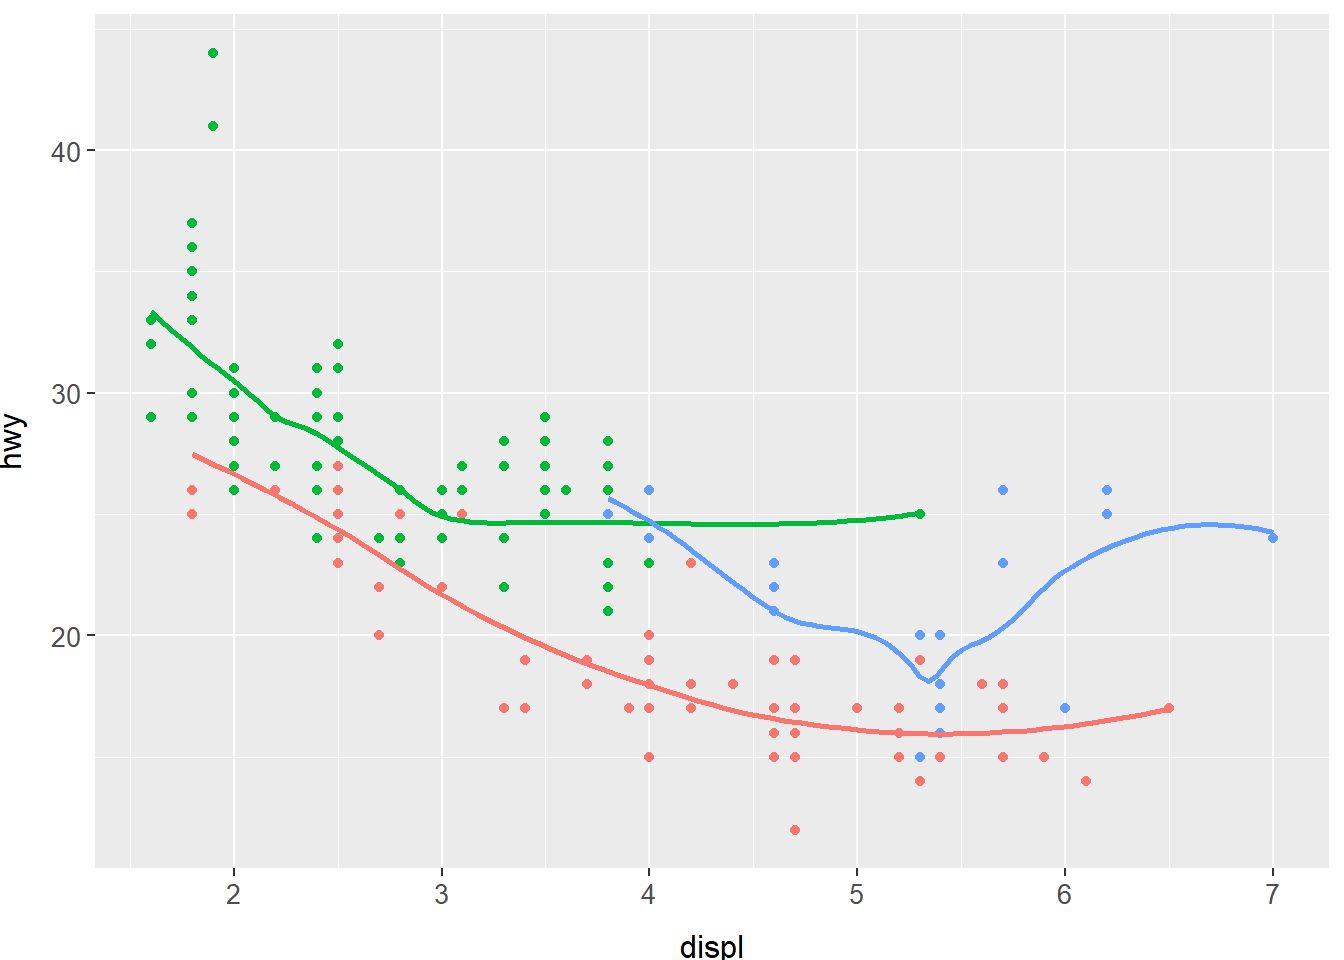
\includegraphics{r4ds_files/figure-latex/unnamed-chunk-27-1.pdf}

Ele indica que, para a camada à qual se aplica, não serão geradas as legendas de identificação.

\end{solution}

\hypertarget{exr1-6-4}{%
\subsection*{Exercício 1.6.4}\label{exr1-6-4}}
\addcontentsline{toc}{subsection}{Exercício 1.6.4}

O que o argumento \texttt{se} para \texttt{geom\_smooth} faz?

\begin{solution}
\leavevmode

\begin{verbatim}
?geom_smooth
\end{verbatim}

Esse argumento indica se o intervalo de confiança utilizado no processo de suavização da linha deve ou não ser exibido no gráfico.

\end{solution}

\hypertarget{exr1-6-5}{%
\subsection*{Exercício 1.6.5}\label{exr1-6-5}}
\addcontentsline{toc}{subsection}{Exercício 1.6.5}

Esses dois gráficos serão diferentes? Por quê/por que não?

\begin{verbatim}
ggplot(data = mpg, mapping = aes(x = displ, y = hwy)) +
    geom_point() +
    geom_smooth() +
    tema
    
ggplot() + 
    geom_point(data = mpg, mapping = aes(x = displ, y = hwy)) +
    geom_smooth(data = mpg, mapping = aes(x = displ, y = hwy)) +
    tema
\end{verbatim}

\begin{solution}
Os gráficos serão iguais. Ao informar os parâmetros \texttt{data} e \texttt{mapping} na função \texttt{ggplot} essas atributos serão considerados como globais, sendo utilizado em todos as camadas do gráfico, a menos que alguma das camadas os sobrescreva. No segundo gráfico, não são definidos parâmetros globais, porém, o mesmo parâmetro é passado para ambas as camadas, sendo assim, a única diferença é o código estar duplicado.
\end{solution}

\hypertarget{exr1-6-6}{%
\subsection*{Exercício 1.6.6}\label{exr1-6-6}}
\addcontentsline{toc}{subsection}{Exercício 1.6.6}

Recrie o código R necessário para gerar os seguintes gráficos:

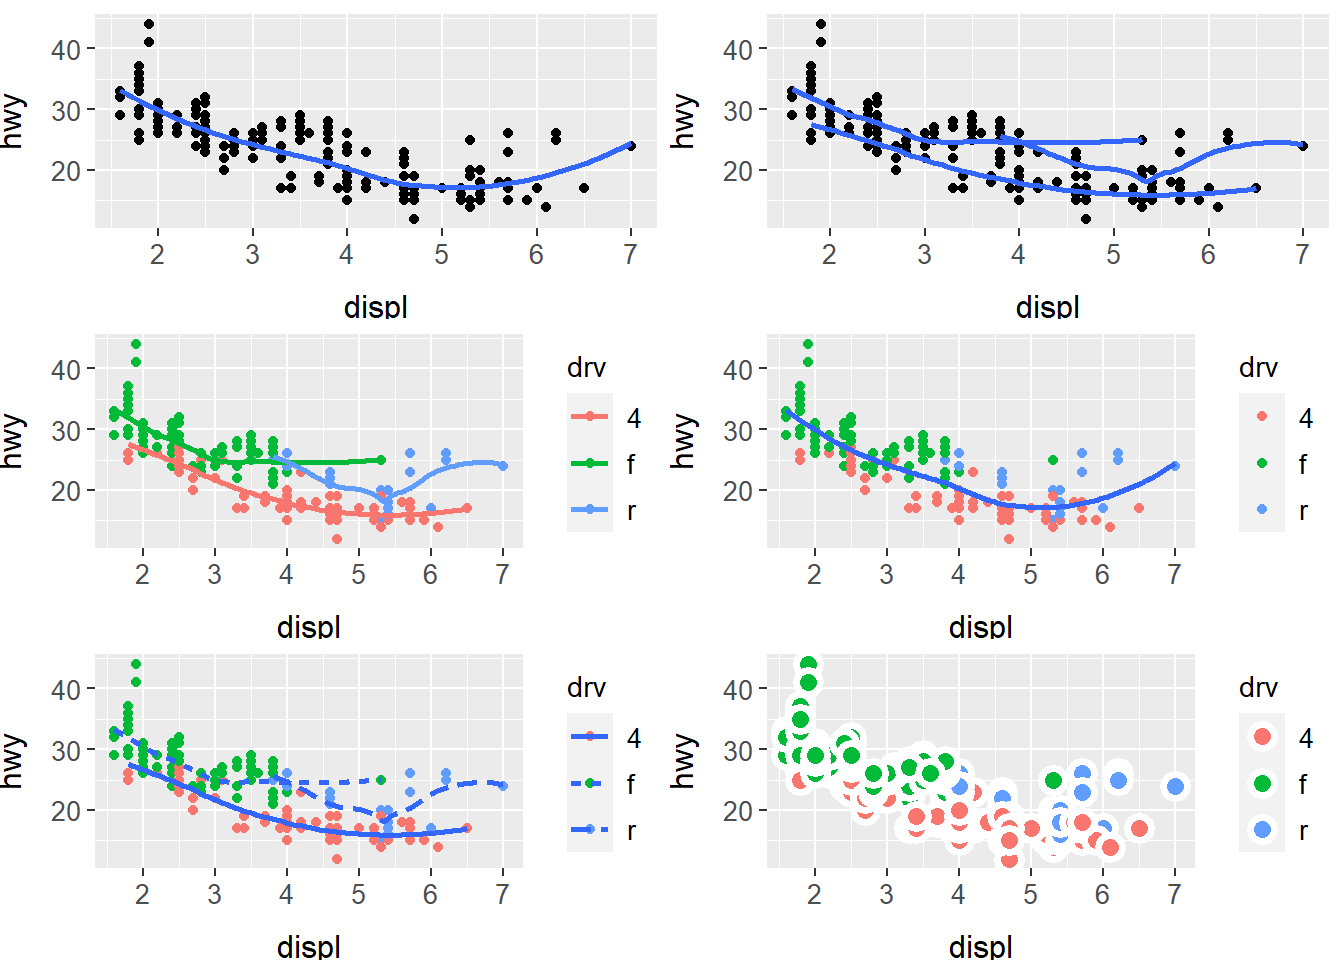
\includegraphics{r4ds_files/figure-latex/unnamed-chunk-28-1.pdf}

\begin{solution}
\leavevmode

\begin{verbatim}
a <- ggplot(data = mpg, mapping = aes(x = displ, y = hwy)) +
        geom_point() +
        geom_smooth(se = FALSE) +
        tema

b <- ggplot(data = mpg, mapping = aes(x = displ, y = hwy)) +
        geom_point() +
        geom_smooth(mapping = aes(group = drv), se = FALSE) +
        tema

c <- ggplot(data = mpg, mapping = aes(x = displ, y = hwy, color = drv)) +
        geom_point() +
        geom_smooth(se = FALSE) +
        tema

d <- ggplot(data = mpg, mapping = aes(x = displ, y = hwy)) +
        geom_point(mapping = aes(color = drv)) +
        geom_smooth(se = FALSE) +
        tema

e <- ggplot(data = mpg, mapping = aes(x = displ, y = hwy)) +
        geom_point(mapping = aes(color = drv)) +
        geom_smooth(mapping = aes(linetype = drv), se = FALSE) +
        tema

f <- ggplot(data = mpg, mapping = aes(x = displ, y = hwy, fill = drv)) +
        geom_point(color = "white", shape = 21, size = 3, stroke = 2) +
        tema
\end{verbatim}

\end{solution}

\hypertarget{transformauxe7uxf5es-estatuxedsticas}{%
\section{Transformações estatísticas}\label{transformauxe7uxf5es-estatuxedsticas}}

\hypertarget{exr1-7-1}{%
\subsection*{Exercício 1.7.1}\label{exr1-7-1}}
\addcontentsline{toc}{subsection}{Exercício 1.7.1}

Qual é o \texttt{geom} padrão associado ao \texttt{stat\_summary()}? Como você poderia reescrever o gráfico anterior usando essa função \texttt{geom}, em vez da função \texttt{stat}?

\begin{solution}
\leavevmode

\begin{verbatim}
?stat_summary
\end{verbatim}

\begin{Shaded}
\begin{Highlighting}[]
\FunctionTok{ggplot}\NormalTok{(}\AttributeTok{data =}\NormalTok{ diamonds) }\SpecialCharTok{+}
    \FunctionTok{stat\_summary}\NormalTok{(}
        \AttributeTok{mapping =} \FunctionTok{aes}\NormalTok{(}\AttributeTok{x =}\NormalTok{ cut, }\AttributeTok{y =}\NormalTok{ depth),}
        \AttributeTok{fun.min =}\NormalTok{ min,}
        \AttributeTok{fun.max =}\NormalTok{ max,}
        \AttributeTok{fun =}\NormalTok{ median}
\NormalTok{    ) }\SpecialCharTok{+}
\NormalTok{    tema}
\end{Highlighting}
\end{Shaded}

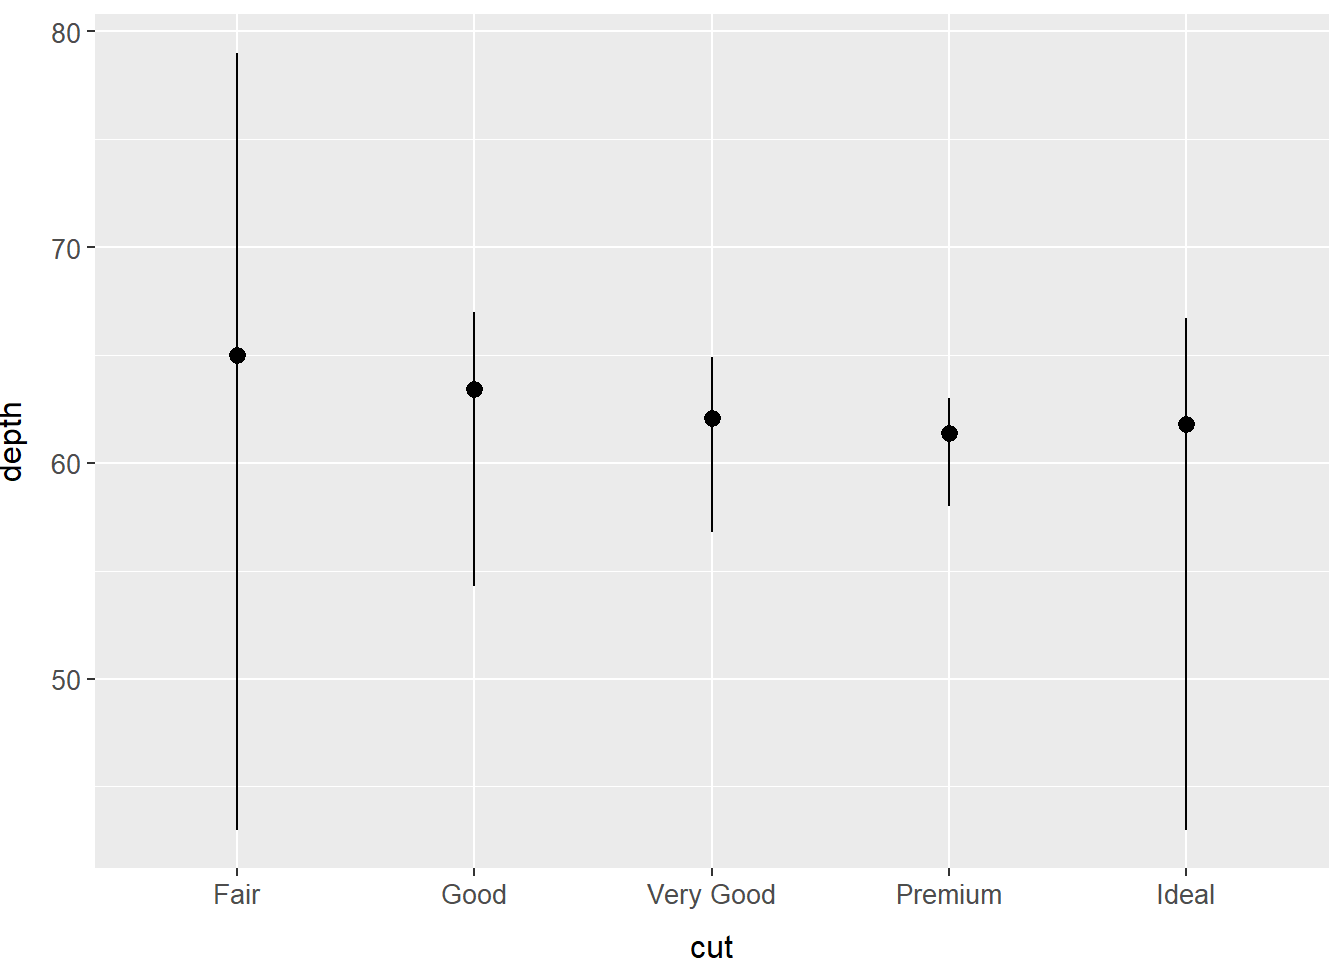
\includegraphics{r4ds_files/figure-latex/unnamed-chunk-29-1.pdf}

A \texttt{geom} associada é a \texttt{geom\_pointrange} e o gráfico poderia ser reescrito da seguinte maneira.

\end{solution}

\hypertarget{exr1-7-2}{%
\subsection*{Exercício 1.7.2}\label{exr1-7-2}}
\addcontentsline{toc}{subsection}{Exercício 1.7.2}

O que \texttt{geom\_col()} faz? Qual é a diferença entre ele e \texttt{geom\_bar()}?

\begin{solution}
\leavevmode

\begin{Shaded}
\begin{Highlighting}[]
\FunctionTok{ggplot}\NormalTok{(}\AttributeTok{data =}\NormalTok{ diamonds, }\AttributeTok{mapping =} \FunctionTok{aes}\NormalTok{(}\AttributeTok{x =}\NormalTok{ cut)) }\SpecialCharTok{+}
    \FunctionTok{geom\_bar}\NormalTok{() }\SpecialCharTok{+}
\NormalTok{    tema}
\end{Highlighting}
\end{Shaded}

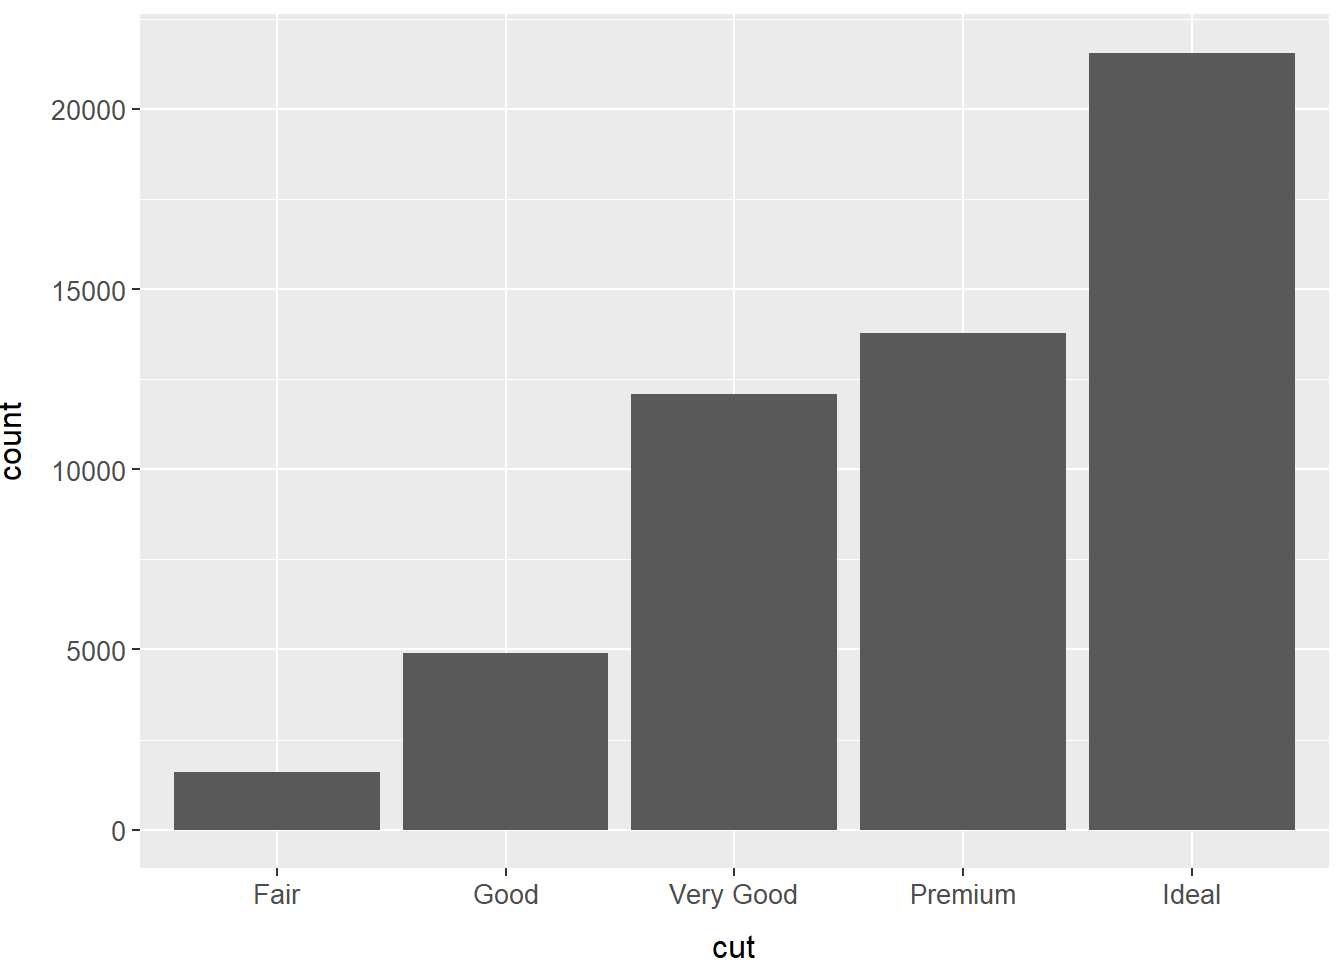
\includegraphics{r4ds_files/figure-latex/unnamed-chunk-30-1.pdf}

\begin{Shaded}
\begin{Highlighting}[]
\FunctionTok{ggplot}\NormalTok{(}\AttributeTok{data =}\NormalTok{ diamonds, }\AttributeTok{mapping =} \FunctionTok{aes}\NormalTok{(}\AttributeTok{x =}\NormalTok{ cut, }\AttributeTok{y =}\NormalTok{ carat)) }\SpecialCharTok{+}
    \FunctionTok{geom\_col}\NormalTok{() }\SpecialCharTok{+}
\NormalTok{    tema}
\end{Highlighting}
\end{Shaded}

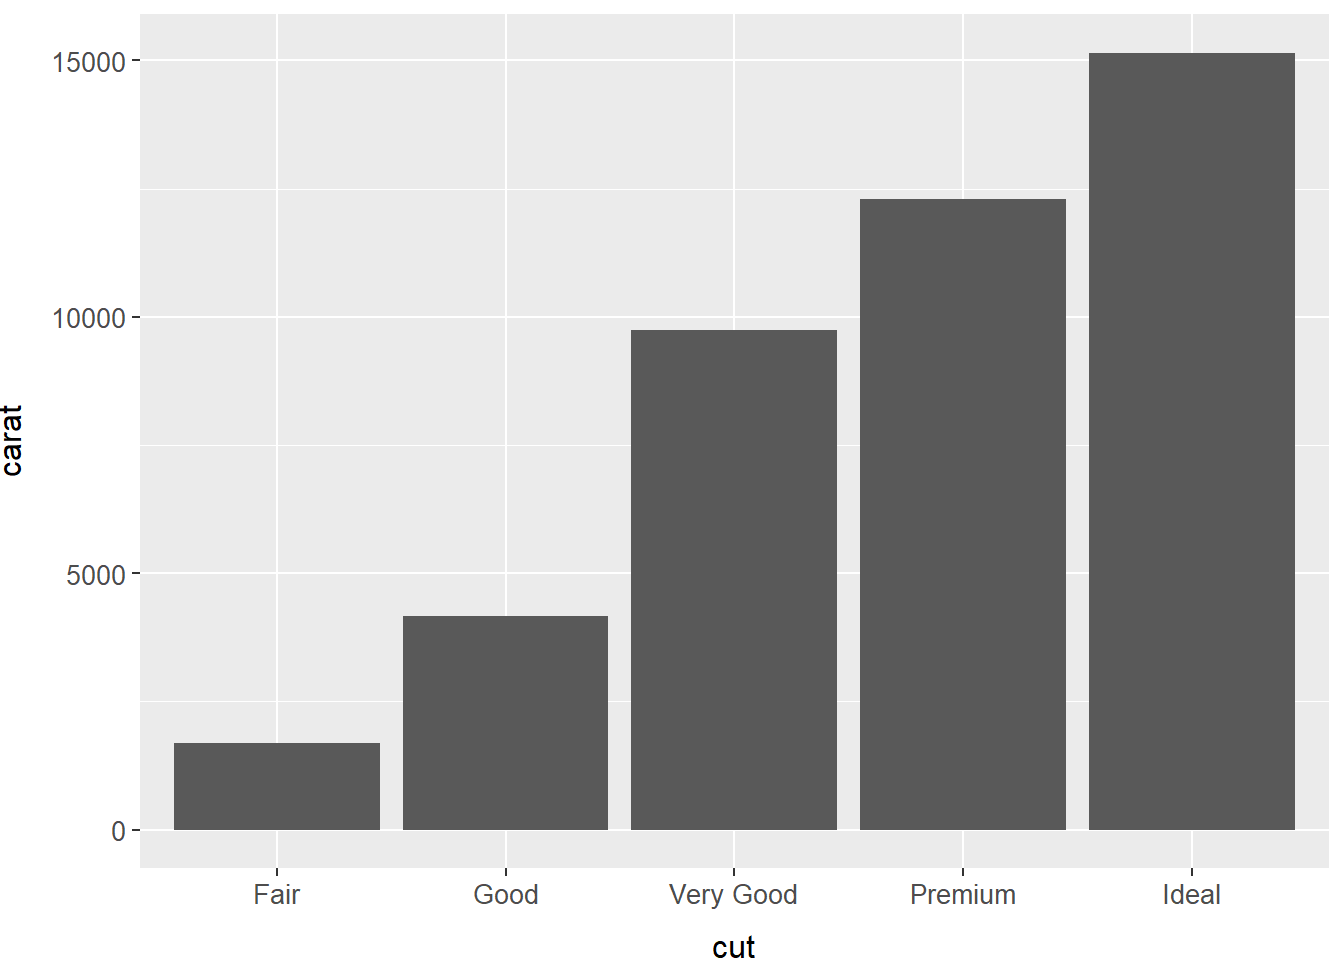
\includegraphics{r4ds_files/figure-latex/unnamed-chunk-31-1.pdf}

Enquanto no \texttt{geom\_bar} a altura das barras representa uma transformação estatística relacionada às observações (como \texttt{count}, por exemplo), no \texttt{geom\_col} podemos exibir o acumulado (soma) de uma variável para cada categoria exibida.

\end{solution}

\hypertarget{exr1-7-3}{%
\subsection*{Exercício 1.7.3}\label{exr1-7-3}}
\addcontentsline{toc}{subsection}{Exercício 1.7.3}

A maioria dos \texttt{geoms} e \texttt{stats} vem em pares, que são quase sempre usados juntos. Leia a documentação e faça uma lista de todos os pares. O que eles têm em comum?

\begin{solution}
\leavevmode

\begin{longtable}[]{@{}ccc@{}}
\toprule\noalign{}
\# & Geom & Stat \\
\midrule\noalign{}
\endhead
\bottomrule\noalign{}
\endlastfoot
01 & Blank & Identity \\
02 & Curve & Identity \\
03 & Segment & Identity \\
04 & Path & Identity \\
05 & Line & Identity \\
06 & Step & Identity \\
07 & Poligon & Identity \\
08 & Raster & Identity \\
09 & Rect & Identity \\
10 & Tile & Identity \\
11 & Ribbon & Identity \\
12 & Area & Identity \\
13 & Align & ? \\
14 & ABLine & ? \\
15 & HLine & ? \\
16 & Density & Density \\
17 & DotPlot & ? \\
18 & Freqpoly & Bin \\
19 & Histogram & Bin \\
20 & Col & Identity \\
21 & Bar & Count \\
22 & Label & Identity \\
23 & Text & Identity \\
24 & Jitter & Identity \\
25 & Point & Identity \\
26 & Quantile & Quantile \\
27 & Rug & Identity \\
28 & Boxplot & Boxplot \\
29 & Violin & YDensity \\
30 & Count & Sum \\
31 & Bin 2D & Bin 2D \\
32 & Density 2D & Density 2D \\
33 & Hex & Bin Hex \\
34 & Cross Bar & Identity \\
35 & Error Bar & Identity \\
36 & Line Range & Identity \\
37 & Point Range & Identity \\
38 & Map & Identity \\
39 & Contour & Contour \\
40 & Contour Filled & Contour Filled \\
\end{longtable}

\end{solution}

\hypertarget{exr1-7-4}{%
\subsection*{Exercício 1.7.4}\label{exr1-7-4}}
\addcontentsline{toc}{subsection}{Exercício 1.7.4}

Quais variáveis \texttt{stat\_smooth()} calcula? Quais parâmetros controlam seu comportamento?

\begin{solution}
\leavevmode

\begin{verbatim}
?stat_smooth
\end{verbatim}

\end{solution}

\hypertarget{exr1-7-5}{%
\subsection*{Exercício 1.7.5}\label{exr1-7-5}}
\addcontentsline{toc}{subsection}{Exercício 1.7.5}

Em nosso gráfico de barra de \emph{proportion}, precisamos configurar \texttt{group\ =\ 1}. Por quê? Em outras palavras, qual é o problema com esses dois gráficos?

\begin{Shaded}
\begin{Highlighting}[]
\FunctionTok{ggplot}\NormalTok{(}\AttributeTok{data =}\NormalTok{ diamonds) }\SpecialCharTok{+}
    \FunctionTok{geom\_bar}\NormalTok{(}\AttributeTok{mapping =} \FunctionTok{aes}\NormalTok{(}\AttributeTok{x =}\NormalTok{ cut, }\AttributeTok{y =} \FunctionTok{after\_stat}\NormalTok{(prop), }\AttributeTok{group =} \DecValTok{1}\NormalTok{)) }\SpecialCharTok{+}
\NormalTok{    tema}
\end{Highlighting}
\end{Shaded}

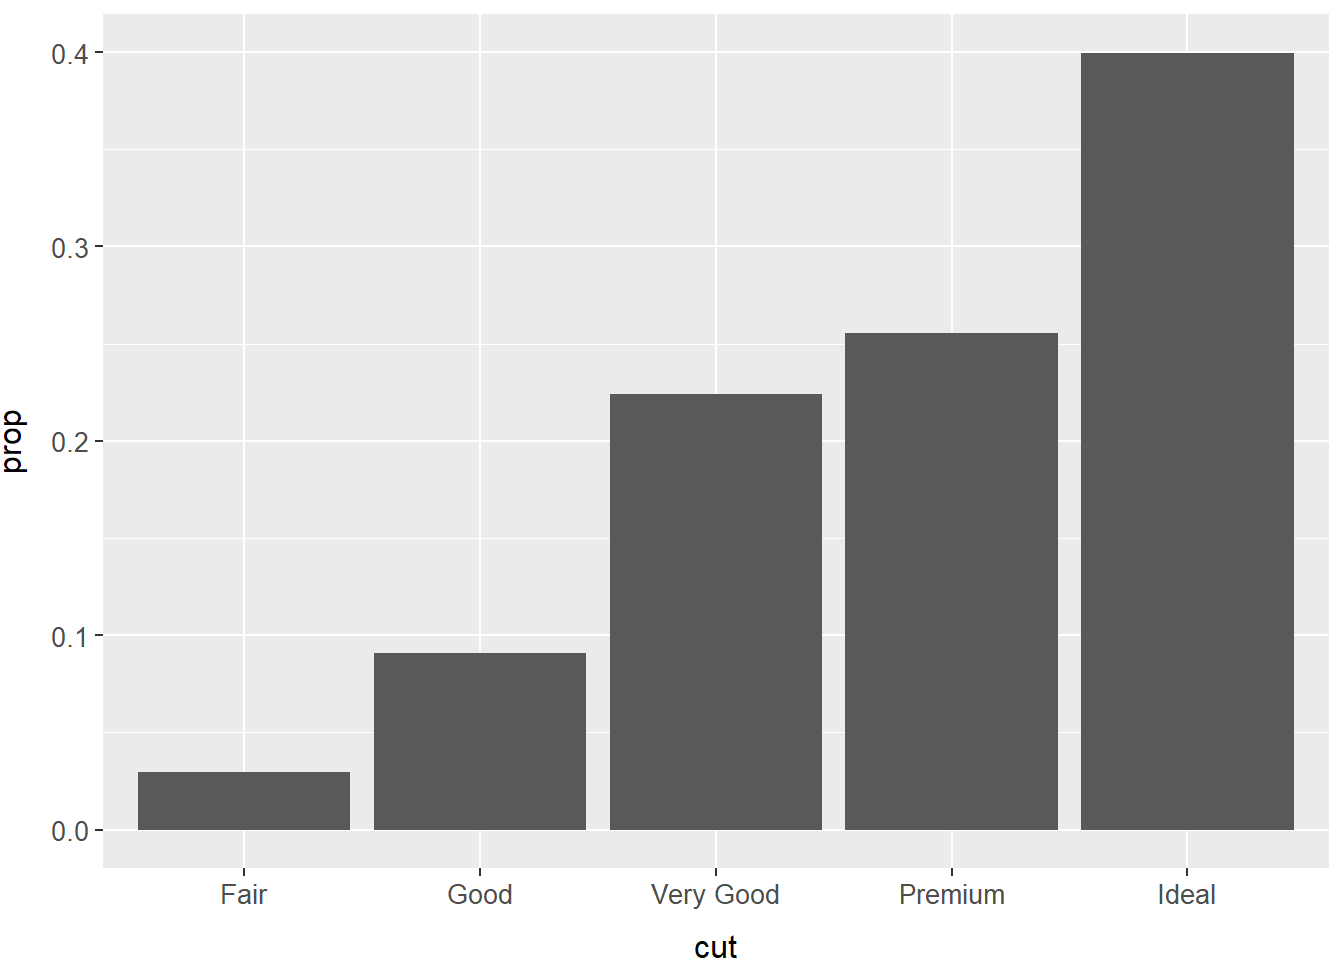
\includegraphics{r4ds_files/figure-latex/unnamed-chunk-32-1.pdf}

\begin{solution}
\leavevmode

\begin{Shaded}
\begin{Highlighting}[]
\FunctionTok{ggplot}\NormalTok{(}\AttributeTok{data =}\NormalTok{ diamonds) }\SpecialCharTok{+}
    \FunctionTok{geom\_bar}\NormalTok{(}\AttributeTok{mapping =} \FunctionTok{aes}\NormalTok{(}
        \AttributeTok{x =}\NormalTok{ cut, }
        \AttributeTok{fill =}\NormalTok{ color, }
        \AttributeTok{y =} \FunctionTok{after\_stat}\NormalTok{(prop), }
        \AttributeTok{group =}\NormalTok{ color}
\NormalTok{    )) }\SpecialCharTok{+}
\NormalTok{    tema}
\end{Highlighting}
\end{Shaded}

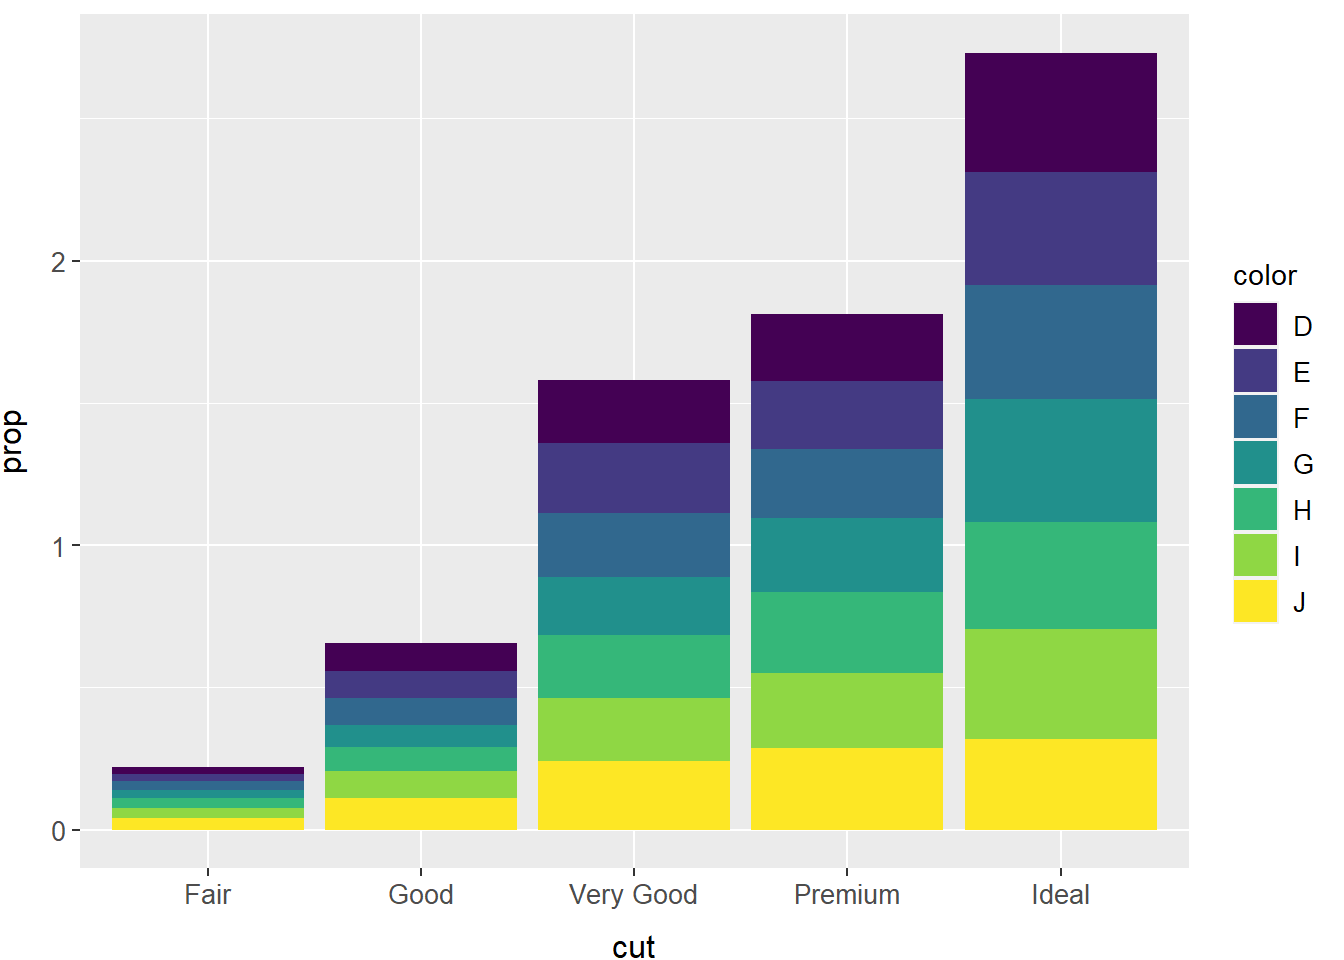
\includegraphics{r4ds_files/figure-latex/unnamed-chunk-33-1.pdf}

Quando estamos trabalhando com proporções (ou estátisticas em geral), é importante destacar para o \texttt{ggplot} qual agrupamento ele deve considerar, caso contrário ele irá considerar um único grupo e dará uma impressão incorreta ao gráfico. No primeiro exemplo, foi utilizado \texttt{group\ =\ 1} (e, na verdade, poderia ser qualquer valor) apenas para indicar que deveria ser realizado um agrupamento.

\end{solution}

\hypertarget{ajustes-de-posiuxe7uxe3o}{%
\section{Ajustes de posição}\label{ajustes-de-posiuxe7uxe3o}}

\hypertarget{exr1-8-1}{%
\subsection*{Exercício 1.8.1}\label{exr1-8-1}}
\addcontentsline{toc}{subsection}{Exercício 1.8.1}

Qual é o problema com este gráfico? Como você poderia melhorá-lo?

\begin{Shaded}
\begin{Highlighting}[]
\FunctionTok{ggplot}\NormalTok{(}\AttributeTok{data =}\NormalTok{ mpg, }\AttributeTok{mapping =} \FunctionTok{aes}\NormalTok{(}\AttributeTok{x =}\NormalTok{ cty, }\AttributeTok{y =}\NormalTok{ hwy)) }\SpecialCharTok{+}
    \FunctionTok{geom\_point}\NormalTok{() }\SpecialCharTok{+}
\NormalTok{    tema}
\end{Highlighting}
\end{Shaded}

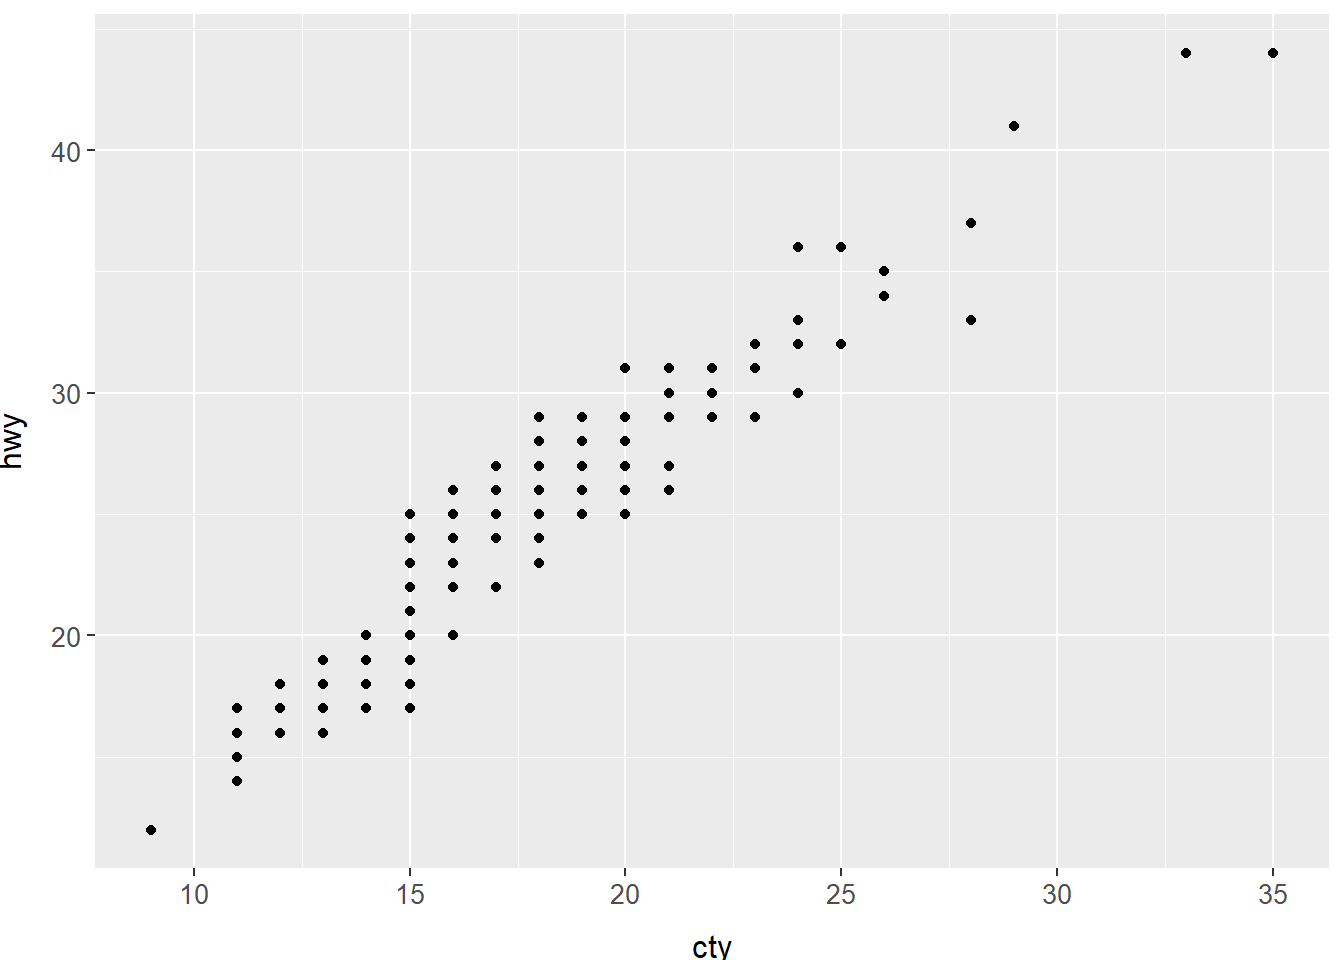
\includegraphics{r4ds_files/figure-latex/unnamed-chunk-34-1.pdf}

\begin{solution}
Há pontos sobrepostos. Uma melhoria poderia ser usar \texttt{geom\_jitter} em lugar de \texttt{geom\_point}.

\begin{Shaded}
\begin{Highlighting}[]
\FunctionTok{ggplot}\NormalTok{(}\AttributeTok{data =}\NormalTok{ mpg, }\AttributeTok{mapping =} \FunctionTok{aes}\NormalTok{(}\AttributeTok{x =}\NormalTok{ cty, }\AttributeTok{y =}\NormalTok{ hwy)) }\SpecialCharTok{+}
    \FunctionTok{geom\_jitter}\NormalTok{() }\SpecialCharTok{+}
\NormalTok{    tema}
\end{Highlighting}
\end{Shaded}

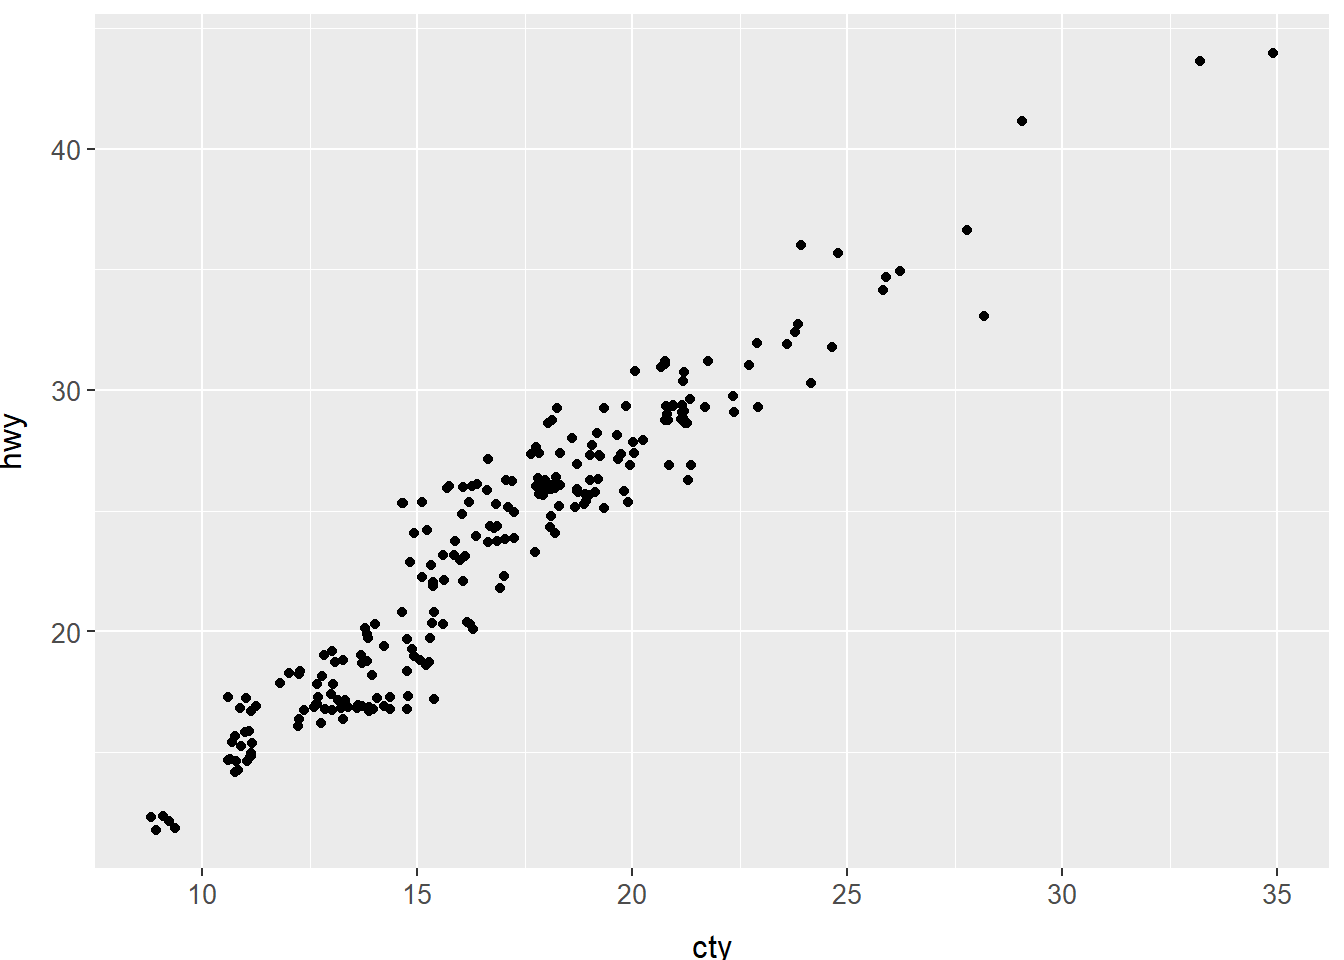
\includegraphics{r4ds_files/figure-latex/unnamed-chunk-35-1.pdf}
\end{solution}

\hypertarget{exr1-8-2}{%
\subsection*{Exercício 1.8.2}\label{exr1-8-2}}
\addcontentsline{toc}{subsection}{Exercício 1.8.2}

Quais parâmetros para \texttt{geom\_jitter} controlam a quantidade de oscilação?

\begin{solution}
Conforme a documentação disposta em \texttt{?geom\_jitter}, são utilizados os parâmetros \texttt{width} e \texttt{height}.
\end{solution}

\hypertarget{exr1-8-3}{%
\subsection*{Exercício 1.8.3}\label{exr1-8-3}}
\addcontentsline{toc}{subsection}{Exercício 1.8.3}

Compare o contraste entre \texttt{geom\_jitter} e \texttt{geom\_count}.

\begin{solution}
\leavevmode

\begin{Shaded}
\begin{Highlighting}[]
\NormalTok{a }\OtherTok{\textless{}{-}} \FunctionTok{ggplot}\NormalTok{(}\AttributeTok{data =}\NormalTok{ mpg, }\AttributeTok{mapping =} \FunctionTok{aes}\NormalTok{(}\AttributeTok{x =}\NormalTok{ cty, }\AttributeTok{y =}\NormalTok{ hwy)) }\SpecialCharTok{+}
      \FunctionTok{geom\_jitter}\NormalTok{() }\SpecialCharTok{+}
\NormalTok{      tema}

\NormalTok{b }\OtherTok{\textless{}{-}} \FunctionTok{ggplot}\NormalTok{(}\AttributeTok{data =}\NormalTok{ mpg, }\AttributeTok{mapping =} \FunctionTok{aes}\NormalTok{(}\AttributeTok{x =}\NormalTok{ cty, }\AttributeTok{y =}\NormalTok{ hwy)) }\SpecialCharTok{+}
      \FunctionTok{geom\_count}\NormalTok{(}\AttributeTok{show.legend =} \ConstantTok{FALSE}\NormalTok{) }\SpecialCharTok{+}
\NormalTok{      tema}

\FunctionTok{grid.arrange}\NormalTok{(a, b, }\AttributeTok{nrow =} \DecValTok{2}\NormalTok{)}
\end{Highlighting}
\end{Shaded}

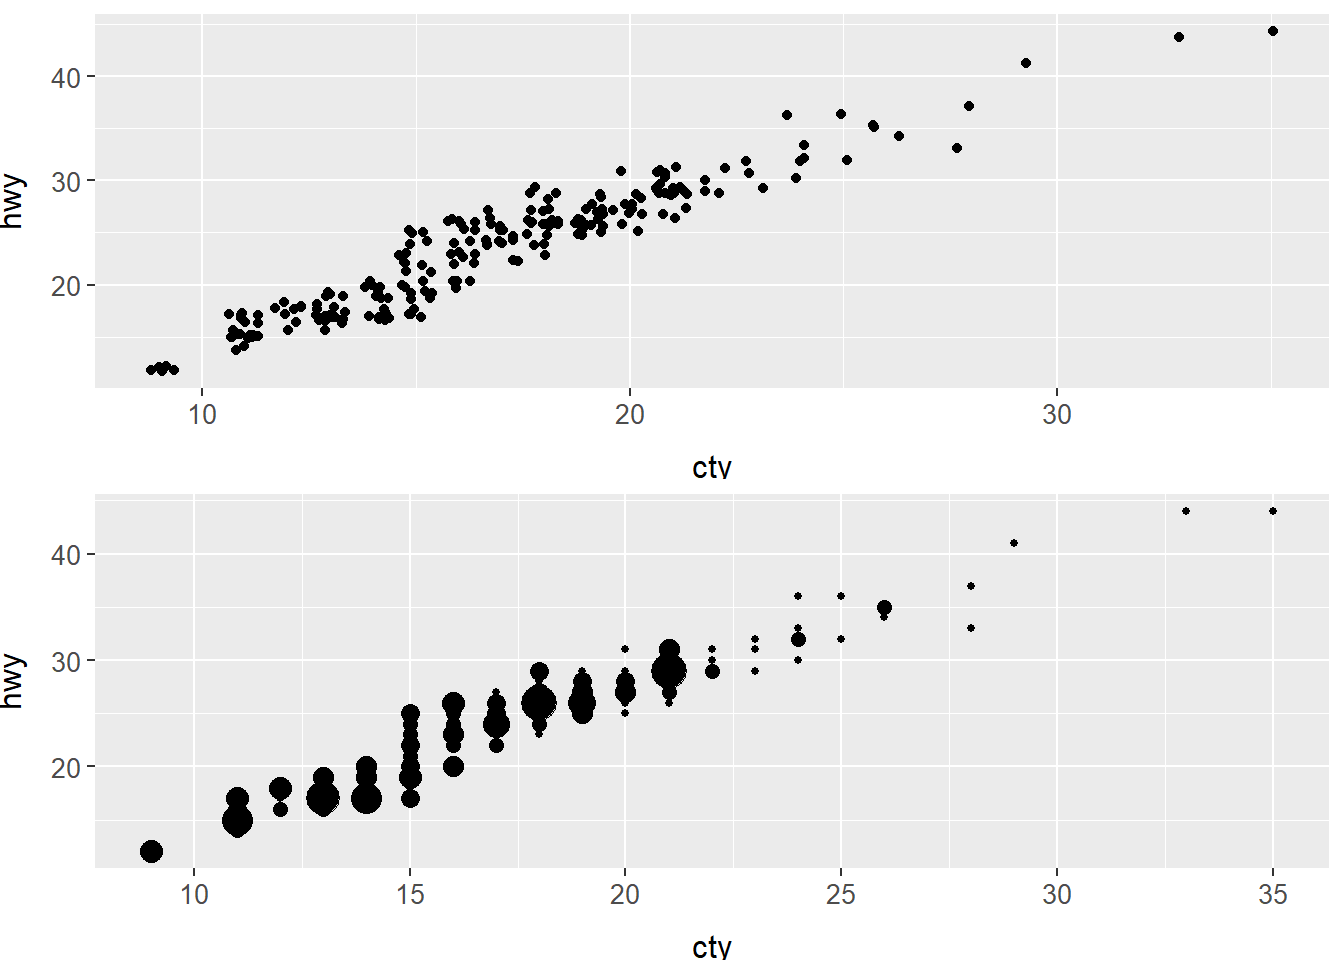
\includegraphics{r4ds_files/figure-latex/unnamed-chunk-36-1.pdf}

Para contornar o problema da sobreposição de pontos, \texttt{geom\_jitter} adiciona um pequeno ruído aleatório aos dados, enquanto o \texttt{geom\_count} contabiliza os pontos sobrepostos e altera o tamanho dos pontos conforme a quantidade.

\end{solution}

\hypertarget{exr1-8-4}{%
\subsection*{Exercício 1.8.4}\label{exr1-8-4}}
\addcontentsline{toc}{subsection}{Exercício 1.8.4}

Qual é o ajuste de posição padrão para \texttt{geom\_boxplot()}? Crie uma visualização do conjunto de dados \texttt{mpg} que demonstre isso.

\begin{solution}
Conforme pode ser visto em \texttt{?geom\_boxplot}, a \texttt{position} padrão é a \texttt{dodge2}.

\begin{Shaded}
\begin{Highlighting}[]
\FunctionTok{ggplot}\NormalTok{(}\AttributeTok{data =}\NormalTok{ mpg, }\AttributeTok{mapping =} \FunctionTok{aes}\NormalTok{(}\AttributeTok{x =}\NormalTok{ class, }\AttributeTok{y =}\NormalTok{ hwy)) }\SpecialCharTok{+}
    \FunctionTok{geom\_boxplot}\NormalTok{() }\SpecialCharTok{+}
\NormalTok{    tema}
\end{Highlighting}
\end{Shaded}

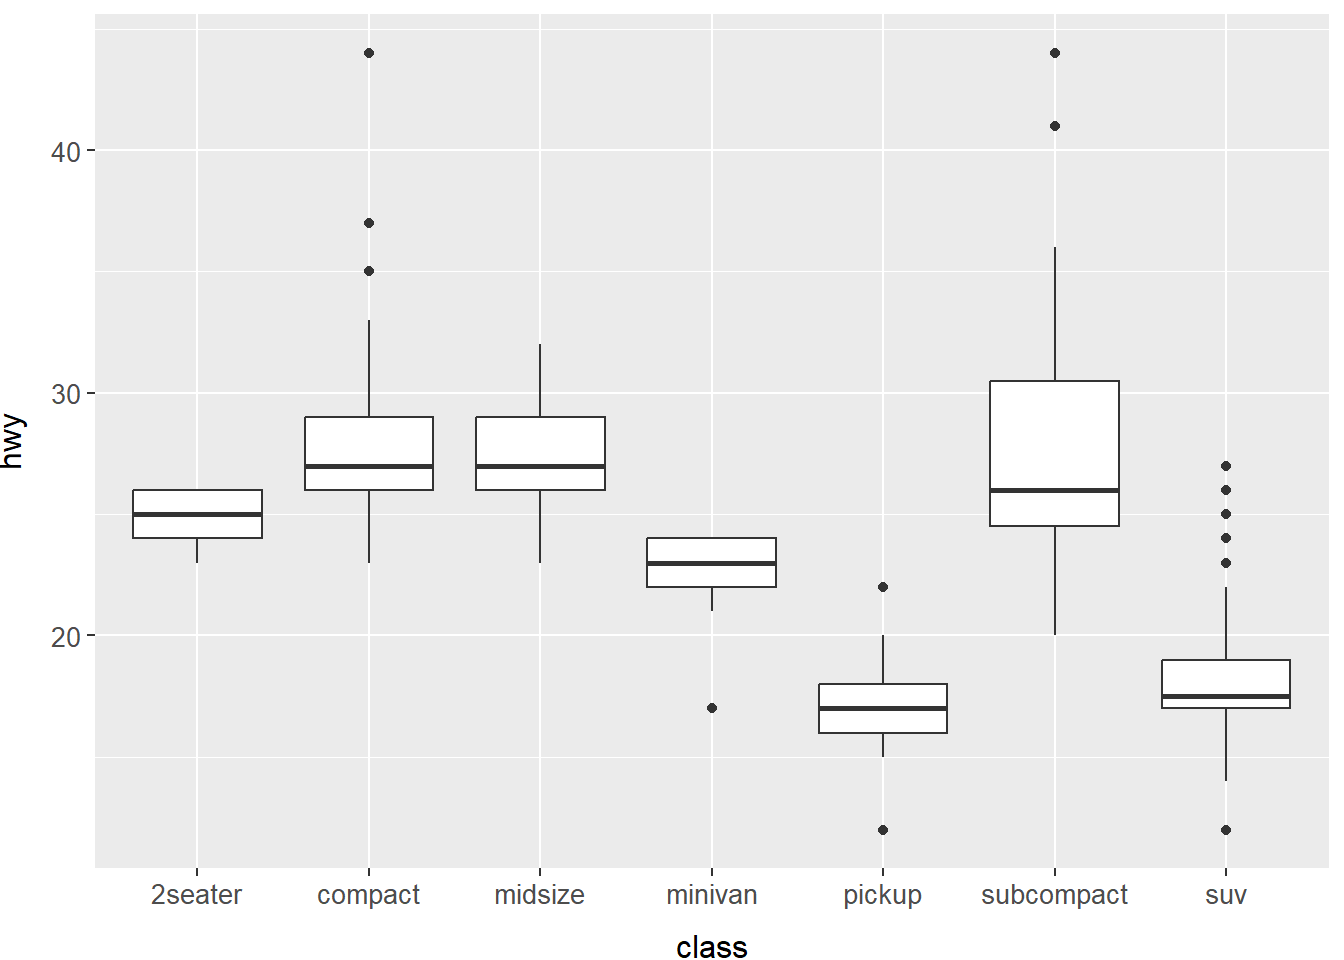
\includegraphics{r4ds_files/figure-latex/unnamed-chunk-37-1.pdf}
\end{solution}

\hypertarget{sistemas-de-coordenadas}{%
\section{Sistemas de coordenadas}\label{sistemas-de-coordenadas}}

\hypertarget{exr1-9-1}{%
\subsection*{Exercício 1.9.1}\label{exr1-9-1}}
\addcontentsline{toc}{subsection}{Exercício 1.9.1}

Transforme um gráfico de barras empilhadas em um gráfico de pizza usando \texttt{coord\_polar()}.

\begin{solution}
\leavevmode

\begin{Shaded}
\begin{Highlighting}[]
\FunctionTok{ggplot}\NormalTok{(}\AttributeTok{data =}\NormalTok{ diamonds, }\AttributeTok{mapping =} \FunctionTok{aes}\NormalTok{(}\AttributeTok{x =}\NormalTok{ cut, }\AttributeTok{fill =}\NormalTok{ cut)) }\SpecialCharTok{+}
    \FunctionTok{geom\_bar}\NormalTok{(}\AttributeTok{show.legend =} \ConstantTok{FALSE}\NormalTok{, }\AttributeTok{width =} \DecValTok{1}\NormalTok{) }\SpecialCharTok{+}
    \FunctionTok{coord\_polar}\NormalTok{() }\SpecialCharTok{+}
    \FunctionTok{labs}\NormalTok{(}\AttributeTok{x =} \ConstantTok{NULL}\NormalTok{, }\AttributeTok{y =} \ConstantTok{NULL}\NormalTok{) }\SpecialCharTok{+}
    \FunctionTok{theme}\NormalTok{(}\AttributeTok{aspect.ratio =} \DecValTok{1}\NormalTok{) }\SpecialCharTok{+}
\NormalTok{    tema}
\end{Highlighting}
\end{Shaded}

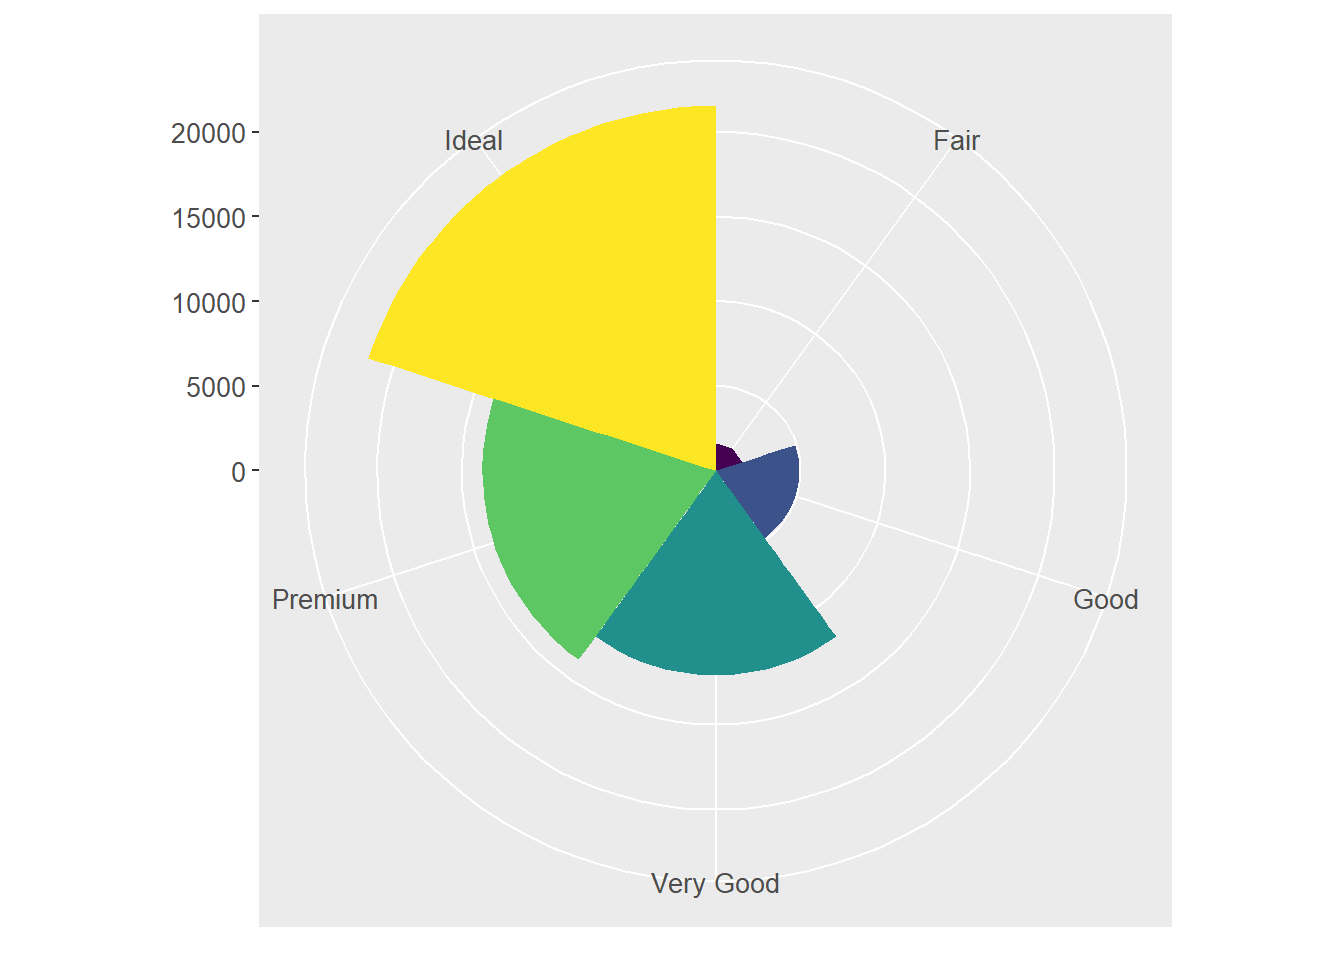
\includegraphics{r4ds_files/figure-latex/unnamed-chunk-38-1.pdf}

\end{solution}

\hypertarget{exr1-9-2}{%
\subsection*{Exercício 1.9.2}\label{exr1-9-2}}
\addcontentsline{toc}{subsection}{Exercício 1.9.2}

O que \texttt{labs()} faz? Leia a documentação.

\begin{solution}
Usando o comando \texttt{?labs}, vimos que esta função é utilizada para definir labels do gráfico, como título, subtítulo, títulos de eixos, etc.
\end{solution}

\hypertarget{exr1-9-3}{%
\subsection*{Exercício 1.9.3}\label{exr1-9-3}}
\addcontentsline{toc}{subsection}{Exercício 1.9.3}

Qual é a diferença entre \texttt{coord\_quickmap()} e \texttt{coord\_map()}?

\begin{solution}
Usando o comando \texttt{?coord\_map}, notamos que a diferença é que enquanto \texttt{coord\_map()} não preserva linhas retas, sendo assim, mais custoso computacionalmente, o \texttt{coord\_quickmap()} o faz.
\end{solution}

\hypertarget{exr1-9-4}{%
\subsection*{Exercício 1.9.4}\label{exr1-9-4}}
\addcontentsline{toc}{subsection}{Exercício 1.9.4}

O que o gráfico a seguir lhe diz sobre a relação entre \texttt{mpg} de cidade e estrada? Por que \texttt{coord\_fixed()} é importante? O que \texttt{geom\_abline()} faz?

\begin{Shaded}
\begin{Highlighting}[]
\FunctionTok{ggplot}\NormalTok{(}\AttributeTok{data =}\NormalTok{ mpg, }\AttributeTok{mapping =} \FunctionTok{aes}\NormalTok{(}\AttributeTok{x =}\NormalTok{ cty, }\AttributeTok{y =}\NormalTok{ hwy)) }\SpecialCharTok{+}
    \FunctionTok{geom\_point}\NormalTok{() }\SpecialCharTok{+}
    \FunctionTok{geom\_abline}\NormalTok{() }\SpecialCharTok{+}
    \FunctionTok{coord\_fixed}\NormalTok{(}\AttributeTok{ratio =} \DecValTok{1}\NormalTok{, }\AttributeTok{xlim =} \FunctionTok{c}\NormalTok{(}\DecValTok{5}\NormalTok{, }\DecValTok{45}\NormalTok{), }\AttributeTok{ylim =} \FunctionTok{c}\NormalTok{(}\DecValTok{5}\NormalTok{, }\DecValTok{45}\NormalTok{)) }\SpecialCharTok{+}
\NormalTok{    tema}
\end{Highlighting}
\end{Shaded}

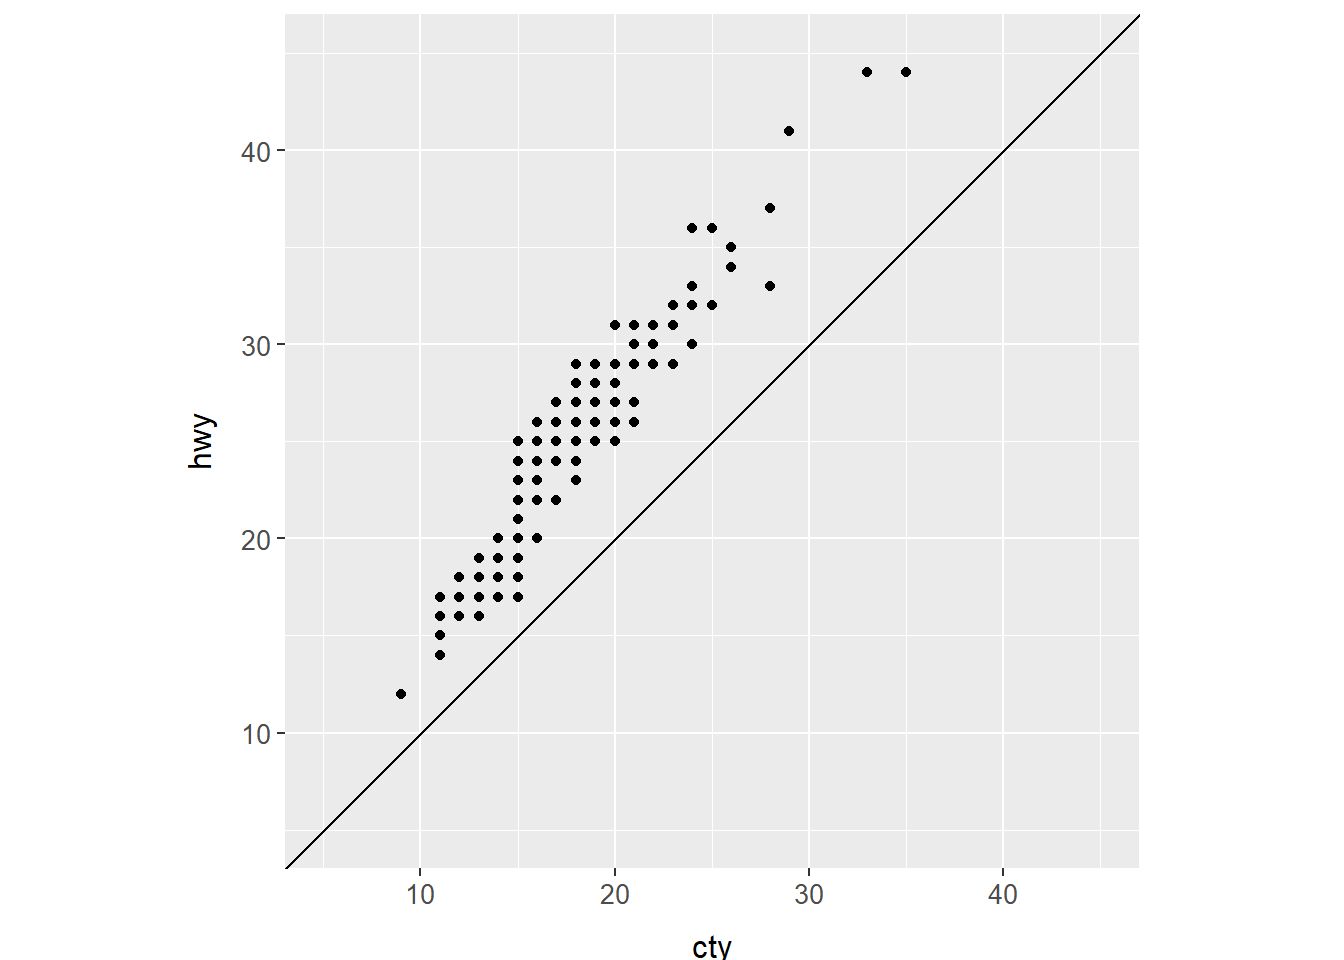
\includegraphics{r4ds_files/figure-latex/unnamed-chunk-39-1.pdf}

\begin{solution}
O gráfico mostra a relação entre a eficiência na cidade e na estrada. O \texttt{coord\_fixed()} força que seja mantida uma proporção entre os eixos x e y, isto é, garante que uma unidade no eixo y corresponda a um número determinado de unidades no eixo x. A razão padrão é 1. Já o \texttt{geom\_abline()} define uma linha de referência diagonal ao gráfico, no nosso caso, a linha é a reta dada por \(y - x = 0\).
\end{solution}

\hypertarget{a-gramuxe1tica-em-camadas-de-gruxe1ficos}{%
\section{A gramática em camadas de gráficos}\label{a-gramuxe1tica-em-camadas-de-gruxe1ficos}}

Não temos exercícios nesta seção.

\hypertarget{fluxo-de-trabalho-o-buxe1sico}{%
\chapter{Fluxo de trabalho: o básico}\label{fluxo-de-trabalho-o-buxe1sico}}

\hypertarget{o-buxe1sico-de-programauxe7uxe3o}{%
\section{O básico de programação}\label{o-buxe1sico-de-programauxe7uxe3o}}

Não temos exercícios nesta seção.

\hypertarget{o-que-huxe1-em-um-nome}{%
\section{O que há em um nome?}\label{o-que-huxe1-em-um-nome}}

Não temos exercícios nesta seção.

\hypertarget{chamando-funuxe7uxf5es}{%
\section{Chamando funções}\label{chamando-funuxe7uxf5es}}

\hypertarget{exr2-3-1}{%
\subsection*{Exercício 2.3.1}\label{exr2-3-1}}
\addcontentsline{toc}{subsection}{Exercício 2.3.1}

Por que esse código não funciona?

\begin{verbatim}
my_variable <- 10
my_varIable
\end{verbatim}

\begin{solution}
Foi atribuído um valor à variável \texttt{my\_variable}, contudo depois tentou-se utilizar essa variável, porém a escrita está incorreta e o \texttt{R} não reconheceu a variável.
O \texttt{R} diferencia letras maiúsculas e minúsculas, isto é, as variáveis \texttt{my\_variable} e \texttt{my\_varIable} são distintas.
\end{solution}

\hypertarget{exr2-3-2}{%
\subsection*{Exercício 2.3.2}\label{exr2-3-2}}
\addcontentsline{toc}{subsection}{Exercício 2.3.2}

Ajuste cada um dos seguintes comandos de \texttt{R} para que executem corretamente.

\begin{verbatim}
library(tidyverse)

ggplot(dota = mpg) +
    geom_point(mapping = aes(x = displ, y = hwy))
    
filter(mpg, cyl = 8)
filter(diamond, carat > 3)
\end{verbatim}

\begin{solution}
\leavevmode

\begin{Shaded}
\begin{Highlighting}[]
\FunctionTok{library}\NormalTok{(tidyverse)}

\FunctionTok{ggplot}\NormalTok{(}\AttributeTok{data =}\NormalTok{ mpg) }\SpecialCharTok{+}
    \FunctionTok{geom\_point}\NormalTok{(}\AttributeTok{mapping =} \FunctionTok{aes}\NormalTok{(}\AttributeTok{x =}\NormalTok{ displ, }\AttributeTok{y =}\NormalTok{ hwy))}
\end{Highlighting}
\end{Shaded}

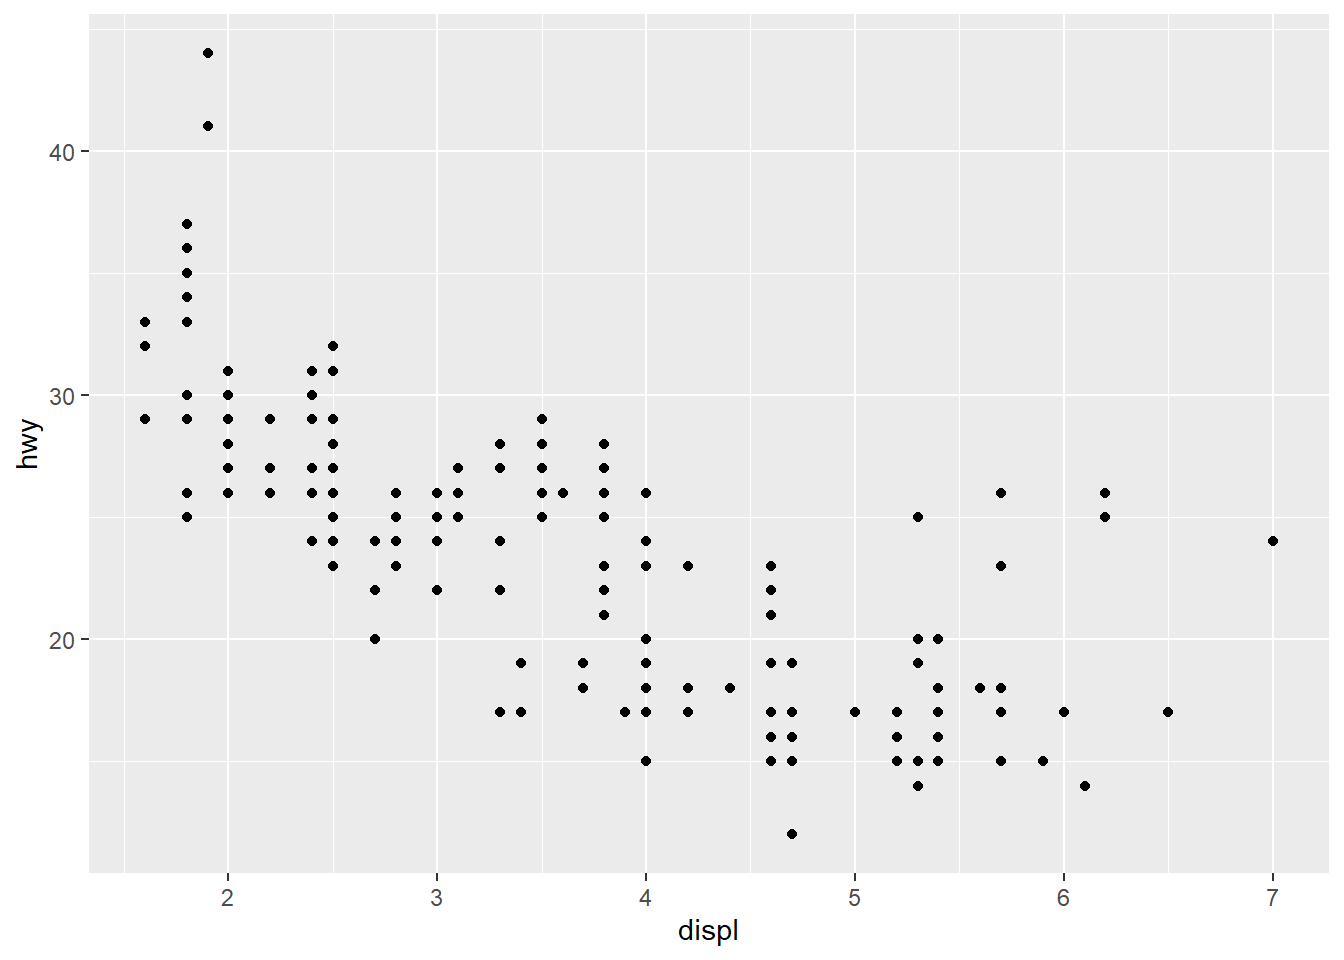
\includegraphics{r4ds_files/figure-latex/unnamed-chunk-40-1.pdf}

\begin{Shaded}
\begin{Highlighting}[]
\FunctionTok{filter}\NormalTok{(mpg, cyl }\SpecialCharTok{==} \DecValTok{8}\NormalTok{)}
\end{Highlighting}
\end{Shaded}

\begin{verbatim}
## # A tibble: 70 x 11
##    manufacturer model      displ  year   cyl trans drv     cty   hwy fl    class
##    <chr>        <chr>      <dbl> <int> <int> <chr> <chr> <int> <int> <chr> <chr>
##  1 audi         a6 quattro   4.2  2008     8 auto~ 4        16    23 p     mids~
##  2 chevrolet    c1500 sub~   5.3  2008     8 auto~ r        14    20 r     suv  
##  3 chevrolet    c1500 sub~   5.3  2008     8 auto~ r        11    15 e     suv  
##  4 chevrolet    c1500 sub~   5.3  2008     8 auto~ r        14    20 r     suv  
##  5 chevrolet    c1500 sub~   5.7  1999     8 auto~ r        13    17 r     suv  
##  6 chevrolet    c1500 sub~   6    2008     8 auto~ r        12    17 r     suv  
##  7 chevrolet    corvette     5.7  1999     8 manu~ r        16    26 p     2sea~
##  8 chevrolet    corvette     5.7  1999     8 auto~ r        15    23 p     2sea~
##  9 chevrolet    corvette     6.2  2008     8 manu~ r        16    26 p     2sea~
## 10 chevrolet    corvette     6.2  2008     8 auto~ r        15    25 p     2sea~
## # i 60 more rows
\end{verbatim}

\begin{Shaded}
\begin{Highlighting}[]
\FunctionTok{filter}\NormalTok{(diamonds, carat }\SpecialCharTok{\textgreater{}} \DecValTok{3}\NormalTok{)}
\end{Highlighting}
\end{Shaded}

\begin{verbatim}
## # A tibble: 32 x 10
##    carat cut     color clarity depth table price     x     y     z
##    <dbl> <ord>   <ord> <ord>   <dbl> <dbl> <int> <dbl> <dbl> <dbl>
##  1  3.01 Premium I     I1       62.7    58  8040  9.1   8.97  5.67
##  2  3.11 Fair    J     I1       65.9    57  9823  9.15  9.02  5.98
##  3  3.01 Premium F     I1       62.2    56  9925  9.24  9.13  5.73
##  4  3.05 Premium E     I1       60.9    58 10453  9.26  9.25  5.66
##  5  3.02 Fair    I     I1       65.2    56 10577  9.11  9.02  5.91
##  6  3.01 Fair    H     I1       56.1    62 10761  9.54  9.38  5.31
##  7  3.65 Fair    H     I1       67.1    53 11668  9.53  9.48  6.38
##  8  3.24 Premium H     I1       62.1    58 12300  9.44  9.4   5.85
##  9  3.22 Ideal   I     I1       62.6    55 12545  9.49  9.42  5.92
## 10  3.5  Ideal   H     I1       62.8    57 12587  9.65  9.59  6.03
## # i 22 more rows
\end{verbatim}

\end{solution}

\hypertarget{exr2-3-3}{%
\subsection*{Exercício 2.3.3}\label{exr2-3-3}}
\addcontentsline{toc}{subsection}{Exercício 2.3.3}

Pressione Alt-Shift-K. O que acontece? Como você pode chegar ao mesmo resultado usando os menus?

\begin{solution}
x
\end{solution}

\hypertarget{transformauxe7uxe3o-de-dados-com-dplyr}{%
\chapter{\texorpdfstring{Transformação de dados com \texttt{dplyr}}{Transformação de dados com dplyr}}\label{transformauxe7uxe3o-de-dados-com-dplyr}}

Para este capítulo, necessitaremos das seguintes configurações iniciais:

\begin{Shaded}
\begin{Highlighting}[]
\NormalTok{not\_cancelled }\OtherTok{\textless{}{-}}\NormalTok{ flights }\SpecialCharTok{\%\textgreater{}\%}
                    \FunctionTok{filter}\NormalTok{(}\SpecialCharTok{!}\FunctionTok{is.na}\NormalTok{(dep\_delay), }\SpecialCharTok{!}\FunctionTok{is.na}\NormalTok{(arr\_delay))}
\end{Highlighting}
\end{Shaded}

\hypertarget{introduuxe7uxe3o-1}{%
\section{Introdução}\label{introduuxe7uxe3o-1}}

Não temos exercícios nesta seção.

\hypertarget{filtrar-linhas-com-filter}{%
\section{\texorpdfstring{Filtrar linhas com \texttt{filter()}}{Filtrar linhas com filter()}}\label{filtrar-linhas-com-filter}}

Não temos exercícios nesta seção.

\hypertarget{comparauxe7uxf5es}{%
\section{Comparações}\label{comparauxe7uxf5es}}

\hypertarget{exr3-3-1}{%
\subsection*{Exercício 3.3.1}\label{exr3-3-1}}
\addcontentsline{toc}{subsection}{Exercício 3.3.1}

Encontre todos os voos que:

\begin{enumerate}
\def\labelenumi{\alph{enumi}.}
\tightlist
\item
  Tiveram um atraso de duas horas ou mais na chegada.
\item
  Foram para Houston (IAH ou HOU).
\item
  Foram operados pela United, American ou Delta.
\item
  Partiram em julho, agosto e setembro.
\item
  Chegaram com mais de duas horas de atraso, mas não saíram atrasados.
\item
  Atrasaram pelo menos uma hora, mas compensaram mais de 30 minutos durante o trajeto.
\item
  Saíram entre meia-noite e 6h (incluindo esses horários).
\end{enumerate}

\begin{solution}
\leavevmode

\begin{enumerate}
\def\labelenumi{\alph{enumi}.}
\tightlist
\item
  Tiveram um atraso de duas horas ou mais na chegada.
\end{enumerate}

\begin{Shaded}
\begin{Highlighting}[]
\FunctionTok{filter}\NormalTok{(flights, arr\_delay }\SpecialCharTok{\textgreater{}=} \DecValTok{120}\NormalTok{)}
\end{Highlighting}
\end{Shaded}

\begin{verbatim}
## # A tibble: 10,200 x 19
##     year month   day dep_time sched_dep_time dep_delay arr_time sched_arr_time
##    <int> <int> <int>    <int>          <int>     <dbl>    <int>          <int>
##  1  2013     1     1      811            630       101     1047            830
##  2  2013     1     1      848           1835       853     1001           1950
##  3  2013     1     1      957            733       144     1056            853
##  4  2013     1     1     1114            900       134     1447           1222
##  5  2013     1     1     1505           1310       115     1638           1431
##  6  2013     1     1     1525           1340       105     1831           1626
##  7  2013     1     1     1549           1445        64     1912           1656
##  8  2013     1     1     1558           1359       119     1718           1515
##  9  2013     1     1     1732           1630        62     2028           1825
## 10  2013     1     1     1803           1620       103     2008           1750
## # i 10,190 more rows
## # i 11 more variables: arr_delay <dbl>, carrier <chr>, flight <int>,
## #   tailnum <chr>, origin <chr>, dest <chr>, air_time <dbl>, distance <dbl>,
## #   hour <dbl>, minute <dbl>, time_hour <dttm>
\end{verbatim}

\begin{enumerate}
\def\labelenumi{\alph{enumi}.}
\setcounter{enumi}{1}
\tightlist
\item
  Foram para Houston (IAH ou HOU).
\end{enumerate}

\begin{Shaded}
\begin{Highlighting}[]
\FunctionTok{filter}\NormalTok{(flights, dest }\SpecialCharTok{\%in\%} \FunctionTok{c}\NormalTok{(}\StringTok{"IAH"}\NormalTok{, }\StringTok{"HOU"}\NormalTok{))}
\end{Highlighting}
\end{Shaded}

\begin{verbatim}
## # A tibble: 9,313 x 19
##     year month   day dep_time sched_dep_time dep_delay arr_time sched_arr_time
##    <int> <int> <int>    <int>          <int>     <dbl>    <int>          <int>
##  1  2013     1     1      517            515         2      830            819
##  2  2013     1     1      533            529         4      850            830
##  3  2013     1     1      623            627        -4      933            932
##  4  2013     1     1      728            732        -4     1041           1038
##  5  2013     1     1      739            739         0     1104           1038
##  6  2013     1     1      908            908         0     1228           1219
##  7  2013     1     1     1028           1026         2     1350           1339
##  8  2013     1     1     1044           1045        -1     1352           1351
##  9  2013     1     1     1114            900       134     1447           1222
## 10  2013     1     1     1205           1200         5     1503           1505
## # i 9,303 more rows
## # i 11 more variables: arr_delay <dbl>, carrier <chr>, flight <int>,
## #   tailnum <chr>, origin <chr>, dest <chr>, air_time <dbl>, distance <dbl>,
## #   hour <dbl>, minute <dbl>, time_hour <dttm>
\end{verbatim}

\begin{enumerate}
\def\labelenumi{\alph{enumi}.}
\setcounter{enumi}{2}
\tightlist
\item
  Foram operados pela United, American ou Delta.
\end{enumerate}

\begin{Shaded}
\begin{Highlighting}[]
\FunctionTok{filter}\NormalTok{(flights, carrier }\SpecialCharTok{\%in\%} \FunctionTok{c}\NormalTok{(}\StringTok{"AA"}\NormalTok{, }\StringTok{"DL"}\NormalTok{, }\StringTok{"UA"}\NormalTok{))}
\end{Highlighting}
\end{Shaded}

\begin{verbatim}
## # A tibble: 139,504 x 19
##     year month   day dep_time sched_dep_time dep_delay arr_time sched_arr_time
##    <int> <int> <int>    <int>          <int>     <dbl>    <int>          <int>
##  1  2013     1     1      517            515         2      830            819
##  2  2013     1     1      533            529         4      850            830
##  3  2013     1     1      542            540         2      923            850
##  4  2013     1     1      554            600        -6      812            837
##  5  2013     1     1      554            558        -4      740            728
##  6  2013     1     1      558            600        -2      753            745
##  7  2013     1     1      558            600        -2      924            917
##  8  2013     1     1      558            600        -2      923            937
##  9  2013     1     1      559            600        -1      941            910
## 10  2013     1     1      559            600        -1      854            902
## # i 139,494 more rows
## # i 11 more variables: arr_delay <dbl>, carrier <chr>, flight <int>,
## #   tailnum <chr>, origin <chr>, dest <chr>, air_time <dbl>, distance <dbl>,
## #   hour <dbl>, minute <dbl>, time_hour <dttm>
\end{verbatim}

\begin{enumerate}
\def\labelenumi{\alph{enumi}.}
\setcounter{enumi}{3}
\tightlist
\item
  Partiram em julho, agosto e setembro.
\end{enumerate}

\begin{Shaded}
\begin{Highlighting}[]
\FunctionTok{filter}\NormalTok{(flights, month }\SpecialCharTok{\%in\%} \FunctionTok{c}\NormalTok{(}\DecValTok{7}\NormalTok{, }\DecValTok{8}\NormalTok{, }\DecValTok{9}\NormalTok{))}
\end{Highlighting}
\end{Shaded}

\begin{verbatim}
## # A tibble: 86,326 x 19
##     year month   day dep_time sched_dep_time dep_delay arr_time sched_arr_time
##    <int> <int> <int>    <int>          <int>     <dbl>    <int>          <int>
##  1  2013     7     1        1           2029       212      236           2359
##  2  2013     7     1        2           2359         3      344            344
##  3  2013     7     1       29           2245       104      151              1
##  4  2013     7     1       43           2130       193      322             14
##  5  2013     7     1       44           2150       174      300            100
##  6  2013     7     1       46           2051       235      304           2358
##  7  2013     7     1       48           2001       287      308           2305
##  8  2013     7     1       58           2155       183      335             43
##  9  2013     7     1      100           2146       194      327             30
## 10  2013     7     1      100           2245       135      337            135
## # i 86,316 more rows
## # i 11 more variables: arr_delay <dbl>, carrier <chr>, flight <int>,
## #   tailnum <chr>, origin <chr>, dest <chr>, air_time <dbl>, distance <dbl>,
## #   hour <dbl>, minute <dbl>, time_hour <dttm>
\end{verbatim}

\begin{enumerate}
\def\labelenumi{\alph{enumi}.}
\setcounter{enumi}{4}
\tightlist
\item
  Chegaram com mais de duas horas de atraso, mas não saíram atrasados.
\end{enumerate}

\begin{Shaded}
\begin{Highlighting}[]
\FunctionTok{filter}\NormalTok{(flights, dep\_delay }\SpecialCharTok{\textless{}=} \DecValTok{0}\NormalTok{, arr\_delay }\SpecialCharTok{\textgreater{}} \DecValTok{120}\NormalTok{)}
\end{Highlighting}
\end{Shaded}

\begin{verbatim}
## # A tibble: 29 x 19
##     year month   day dep_time sched_dep_time dep_delay arr_time sched_arr_time
##    <int> <int> <int>    <int>          <int>     <dbl>    <int>          <int>
##  1  2013     1    27     1419           1420        -1     1754           1550
##  2  2013    10     7     1350           1350         0     1736           1526
##  3  2013    10     7     1357           1359        -2     1858           1654
##  4  2013    10    16      657            700        -3     1258           1056
##  5  2013    11     1      658            700        -2     1329           1015
##  6  2013     3    18     1844           1847        -3       39           2219
##  7  2013     4    17     1635           1640        -5     2049           1845
##  8  2013     4    18      558            600        -2     1149            850
##  9  2013     4    18      655            700        -5     1213            950
## 10  2013     5    22     1827           1830        -3     2217           2010
## # i 19 more rows
## # i 11 more variables: arr_delay <dbl>, carrier <chr>, flight <int>,
## #   tailnum <chr>, origin <chr>, dest <chr>, air_time <dbl>, distance <dbl>,
## #   hour <dbl>, minute <dbl>, time_hour <dttm>
\end{verbatim}

\begin{enumerate}
\def\labelenumi{\alph{enumi}.}
\setcounter{enumi}{5}
\tightlist
\item
  Atrasaram pelo menos uma hora, mas compensaram mais de 30 minutos durante o trajeto.
\end{enumerate}

\begin{Shaded}
\begin{Highlighting}[]
\FunctionTok{filter}\NormalTok{(flights, dep\_delay }\SpecialCharTok{\textgreater{}=} \DecValTok{60} \SpecialCharTok{\&}\NormalTok{ dep\_delay }\SpecialCharTok{{-}}\NormalTok{ arr\_delay }\SpecialCharTok{\textgreater{}=} \DecValTok{30}\NormalTok{)}
\end{Highlighting}
\end{Shaded}

\begin{verbatim}
## # A tibble: 2,074 x 19
##     year month   day dep_time sched_dep_time dep_delay arr_time sched_arr_time
##    <int> <int> <int>    <int>          <int>     <dbl>    <int>          <int>
##  1  2013     1     1     1716           1545        91     2140           2039
##  2  2013     1     1     2205           1720       285       46           2040
##  3  2013     1     1     2326           2130       116      131             18
##  4  2013     1     3     1503           1221       162     1803           1555
##  5  2013     1     3     1821           1530       171     2131           1910
##  6  2013     1     3     1839           1700        99     2056           1950
##  7  2013     1     3     1850           1745        65     2148           2120
##  8  2013     1     3     1923           1815        68     2036           1958
##  9  2013     1     3     1941           1759       102     2246           2139
## 10  2013     1     3     1950           1845        65     2228           2227
## # i 2,064 more rows
## # i 11 more variables: arr_delay <dbl>, carrier <chr>, flight <int>,
## #   tailnum <chr>, origin <chr>, dest <chr>, air_time <dbl>, distance <dbl>,
## #   hour <dbl>, minute <dbl>, time_hour <dttm>
\end{verbatim}

\begin{enumerate}
\def\labelenumi{\alph{enumi}.}
\setcounter{enumi}{6}
\tightlist
\item
  Saíram entre meia-noite e 6h (incluindo esses horários).
\end{enumerate}

\begin{Shaded}
\begin{Highlighting}[]
\FunctionTok{filter}\NormalTok{(flights, dep\_time }\SpecialCharTok{\textgreater{}=} \DecValTok{0}\NormalTok{, dep\_time }\SpecialCharTok{\textless{}=} \DecValTok{600}\NormalTok{)}
\end{Highlighting}
\end{Shaded}

\begin{verbatim}
## # A tibble: 9,344 x 19
##     year month   day dep_time sched_dep_time dep_delay arr_time sched_arr_time
##    <int> <int> <int>    <int>          <int>     <dbl>    <int>          <int>
##  1  2013     1     1      517            515         2      830            819
##  2  2013     1     1      533            529         4      850            830
##  3  2013     1     1      542            540         2      923            850
##  4  2013     1     1      544            545        -1     1004           1022
##  5  2013     1     1      554            600        -6      812            837
##  6  2013     1     1      554            558        -4      740            728
##  7  2013     1     1      555            600        -5      913            854
##  8  2013     1     1      557            600        -3      709            723
##  9  2013     1     1      557            600        -3      838            846
## 10  2013     1     1      558            600        -2      753            745
## # i 9,334 more rows
## # i 11 more variables: arr_delay <dbl>, carrier <chr>, flight <int>,
## #   tailnum <chr>, origin <chr>, dest <chr>, air_time <dbl>, distance <dbl>,
## #   hour <dbl>, minute <dbl>, time_hour <dttm>
\end{verbatim}

\end{solution}

\hypertarget{exr3-3-2}{%
\subsection*{Exercício 3.3.2}\label{exr3-3-2}}
\addcontentsline{toc}{subsection}{Exercício 3.3.2}

Outro ajudante da filtragem do \textbf{dplyr} é \texttt{between()}. O que ele faz? Você consegue utilizá-lo para simplificar o código necessário para responder os desafios anteriores?

\begin{solution}

O \texttt{between} recebe três parâmetros e verifica se o primeiro está entre o segundo e o terceiro.

\begin{Shaded}
\begin{Highlighting}[]
\FunctionTok{filter}\NormalTok{(flights, }\FunctionTok{between}\NormalTok{(dep\_time, }\DecValTok{0}\NormalTok{, }\DecValTok{600}\NormalTok{))}
\end{Highlighting}
\end{Shaded}

\begin{verbatim}
## # A tibble: 9,344 x 19
##     year month   day dep_time sched_dep_time dep_delay arr_time sched_arr_time
##    <int> <int> <int>    <int>          <int>     <dbl>    <int>          <int>
##  1  2013     1     1      517            515         2      830            819
##  2  2013     1     1      533            529         4      850            830
##  3  2013     1     1      542            540         2      923            850
##  4  2013     1     1      544            545        -1     1004           1022
##  5  2013     1     1      554            600        -6      812            837
##  6  2013     1     1      554            558        -4      740            728
##  7  2013     1     1      555            600        -5      913            854
##  8  2013     1     1      557            600        -3      709            723
##  9  2013     1     1      557            600        -3      838            846
## 10  2013     1     1      558            600        -2      753            745
## # i 9,334 more rows
## # i 11 more variables: arr_delay <dbl>, carrier <chr>, flight <int>,
## #   tailnum <chr>, origin <chr>, dest <chr>, air_time <dbl>, distance <dbl>,
## #   hour <dbl>, minute <dbl>, time_hour <dttm>
\end{verbatim}

\end{solution}

\hypertarget{exr3-3-3}{%
\subsection*{Exercício 3.3.3}\label{exr3-3-3}}
\addcontentsline{toc}{subsection}{Exercício 3.3.3}

Quantos voos têm um \texttt{dep\_time} faltante? Que outras variáveis estão faltando? O que essas linhas podem representar?

\begin{solution}
\leavevmode

\begin{Shaded}
\begin{Highlighting}[]
\FunctionTok{count}\NormalTok{(flights, }\FunctionTok{is.na}\NormalTok{(dep\_time))}
\end{Highlighting}
\end{Shaded}

\begin{verbatim}
## # A tibble: 2 x 2
##   `is.na(dep_time)`      n
##   <lgl>              <int>
## 1 FALSE             328521
## 2 TRUE                8255
\end{verbatim}

\begin{Shaded}
\begin{Highlighting}[]
\FunctionTok{summary}\NormalTok{(}\FunctionTok{is.na}\NormalTok{(flights))}
\end{Highlighting}
\end{Shaded}

\begin{verbatim}
##     year           month            day           dep_time      
##  Mode :logical   Mode :logical   Mode :logical   Mode :logical  
##  FALSE:336776    FALSE:336776    FALSE:336776    FALSE:328521   
##                                                  TRUE :8255     
##  sched_dep_time  dep_delay        arr_time       sched_arr_time 
##  Mode :logical   Mode :logical   Mode :logical   Mode :logical  
##  FALSE:336776    FALSE:328521    FALSE:328063    FALSE:336776   
##                  TRUE :8255      TRUE :8713                     
##  arr_delay        carrier          flight         tailnum       
##  Mode :logical   Mode :logical   Mode :logical   Mode :logical  
##  FALSE:327346    FALSE:336776    FALSE:336776    FALSE:334264   
##  TRUE :9430                                      TRUE :2512     
##    origin           dest          air_time        distance      
##  Mode :logical   Mode :logical   Mode :logical   Mode :logical  
##  FALSE:336776    FALSE:336776    FALSE:327346    FALSE:336776   
##                                  TRUE :9430                     
##     hour           minute        time_hour      
##  Mode :logical   Mode :logical   Mode :logical  
##  FALSE:336776    FALSE:336776    FALSE:336776   
## 
\end{verbatim}

São 8255 voos com \texttt{dep\_time} faltante, o que pode indicar voos cancelados. As seguintes colunas também possuem dados faltantes: \texttt{dep\_delay}, \texttt{arr\_time}, \texttt{arr\_delay}, \texttt{tailnum} e \texttt{air\_time}.

\end{solution}

\hypertarget{exr3-3-4}{%
\subsection*{Exercício 3.3.4}\label{exr3-3-4}}
\addcontentsline{toc}{subsection}{Exercício 3.3.4}

Por que \texttt{NA\ \^{}\ 0} não é um valor faltante? Por que \texttt{NA\ \textbar{}\ TRUE} não é um valor faltante? Por que \texttt{FALSE\ \&\ NA} não é um valor faltante? Você consegue descobrir a regra geral? (\texttt{NA\ *\ 0} é um contraexemplo complicado!)

\begin{solution}
\texttt{NA\ \^{}\ 0} resulta em um, pois qualquer número real satisfaz essa mesma condição. A regra geral parece ser que, ao avaliar a expressão, sempre que o valor que \texttt{NA} representaria for indiferente para o resultado da expressão, então será retornado um valor diferente de \texttt{NA}.
\end{solution}

\hypertarget{ordenar-linhas-com-arrange}{%
\section{\texorpdfstring{Ordenar linhas com \texttt{arrange()}}{Ordenar linhas com arrange()}}\label{ordenar-linhas-com-arrange}}

\hypertarget{exr3-4-1}{%
\subsection*{Exercício 3.4.1}\label{exr3-4-1}}
\addcontentsline{toc}{subsection}{Exercício 3.4.1}

Como você poderia usar \texttt{arrange()} para classificar todos os valores faltantes no começo? (dica: use \texttt{is.na()}.)

\begin{solution}
\leavevmode

\begin{Shaded}
\begin{Highlighting}[]
\FunctionTok{arrange}\NormalTok{(}
\NormalTok{  flights, }
  \SpecialCharTok{!}\FunctionTok{is.na}\NormalTok{(year), }
  \SpecialCharTok{!}\FunctionTok{is.na}\NormalTok{(month), }
  \SpecialCharTok{!}\FunctionTok{is.na}\NormalTok{(day), }
  \SpecialCharTok{!}\FunctionTok{is.na}\NormalTok{(dep\_time), }
  \SpecialCharTok{!}\FunctionTok{is.na}\NormalTok{(sched\_dep\_time), }
  \SpecialCharTok{!}\FunctionTok{is.na}\NormalTok{(dep\_delay), }
  \SpecialCharTok{!}\FunctionTok{is.na}\NormalTok{(arr\_time), }
  \SpecialCharTok{!}\FunctionTok{is.na}\NormalTok{(sched\_arr\_time), }
  \SpecialCharTok{!}\FunctionTok{is.na}\NormalTok{(arr\_delay), }
  \SpecialCharTok{!}\FunctionTok{is.na}\NormalTok{(carrier), }
  \SpecialCharTok{!}\FunctionTok{is.na}\NormalTok{(flight), }
  \SpecialCharTok{!}\FunctionTok{is.na}\NormalTok{(tailnum), }
  \SpecialCharTok{!}\FunctionTok{is.na}\NormalTok{(origin), }
  \SpecialCharTok{!}\FunctionTok{is.na}\NormalTok{(dest), }
  \SpecialCharTok{!}\FunctionTok{is.na}\NormalTok{(air\_time), }
  \SpecialCharTok{!}\FunctionTok{is.na}\NormalTok{(distance), }
  \SpecialCharTok{!}\FunctionTok{is.na}\NormalTok{(hour), }
  \SpecialCharTok{!}\FunctionTok{is.na}\NormalTok{(minute), }
  \SpecialCharTok{!}\FunctionTok{is.na}\NormalTok{(time\_hour)}
\NormalTok{)}
\end{Highlighting}
\end{Shaded}

\begin{verbatim}
## # A tibble: 336,776 x 19
##     year month   day dep_time sched_dep_time dep_delay arr_time sched_arr_time
##    <int> <int> <int>    <int>          <int>     <dbl>    <int>          <int>
##  1  2013     1     2       NA           1545        NA       NA           1910
##  2  2013     1     2       NA           1601        NA       NA           1735
##  3  2013     1     3       NA            857        NA       NA           1209
##  4  2013     1     3       NA            645        NA       NA            952
##  5  2013     1     4       NA            845        NA       NA           1015
##  6  2013     1     4       NA           1830        NA       NA           2044
##  7  2013     1     5       NA            840        NA       NA           1001
##  8  2013     1     7       NA            820        NA       NA            958
##  9  2013     1     8       NA           1645        NA       NA           1838
## 10  2013     1     9       NA            755        NA       NA           1012
## # i 336,766 more rows
## # i 11 more variables: arr_delay <dbl>, carrier <chr>, flight <int>,
## #   tailnum <chr>, origin <chr>, dest <chr>, air_time <dbl>, distance <dbl>,
## #   hour <dbl>, minute <dbl>, time_hour <dttm>
\end{verbatim}

\end{solution}

\begin{remark}
Deve haver uma solução muito mais elegante para este problema.
\end{remark}

\hypertarget{exr3-4-2}{%
\subsection*{Exercício 3.4.2}\label{exr3-4-2}}
\addcontentsline{toc}{subsection}{Exercício 3.4.2}

Ordene \texttt{flights} para encontrar os voos mais atrasados. Encontre os voos que saíram mais cedo.

\begin{solution}

Voos mais atrasados:

\begin{Shaded}
\begin{Highlighting}[]
\FunctionTok{arrange}\NormalTok{(flights, }\FunctionTok{desc}\NormalTok{(dep\_delay))}
\end{Highlighting}
\end{Shaded}

\begin{verbatim}
## # A tibble: 336,776 x 19
##     year month   day dep_time sched_dep_time dep_delay arr_time sched_arr_time
##    <int> <int> <int>    <int>          <int>     <dbl>    <int>          <int>
##  1  2013     1     9      641            900      1301     1242           1530
##  2  2013     6    15     1432           1935      1137     1607           2120
##  3  2013     1    10     1121           1635      1126     1239           1810
##  4  2013     9    20     1139           1845      1014     1457           2210
##  5  2013     7    22      845           1600      1005     1044           1815
##  6  2013     4    10     1100           1900       960     1342           2211
##  7  2013     3    17     2321            810       911      135           1020
##  8  2013     6    27      959           1900       899     1236           2226
##  9  2013     7    22     2257            759       898      121           1026
## 10  2013    12     5      756           1700       896     1058           2020
## # i 336,766 more rows
## # i 11 more variables: arr_delay <dbl>, carrier <chr>, flight <int>,
## #   tailnum <chr>, origin <chr>, dest <chr>, air_time <dbl>, distance <dbl>,
## #   hour <dbl>, minute <dbl>, time_hour <dttm>
\end{verbatim}

Voos que saíram mais cedo:

\begin{Shaded}
\begin{Highlighting}[]
\FunctionTok{arrange}\NormalTok{(flights, dep\_time)}
\end{Highlighting}
\end{Shaded}

\begin{verbatim}
## # A tibble: 336,776 x 19
##     year month   day dep_time sched_dep_time dep_delay arr_time sched_arr_time
##    <int> <int> <int>    <int>          <int>     <dbl>    <int>          <int>
##  1  2013     1    13        1           2249        72      108           2357
##  2  2013     1    31        1           2100       181      124           2225
##  3  2013    11    13        1           2359         2      442            440
##  4  2013    12    16        1           2359         2      447            437
##  5  2013    12    20        1           2359         2      430            440
##  6  2013    12    26        1           2359         2      437            440
##  7  2013    12    30        1           2359         2      441            437
##  8  2013     2    11        1           2100       181      111           2225
##  9  2013     2    24        1           2245        76      121           2354
## 10  2013     3     8        1           2355         6      431            440
## # i 336,766 more rows
## # i 11 more variables: arr_delay <dbl>, carrier <chr>, flight <int>,
## #   tailnum <chr>, origin <chr>, dest <chr>, air_time <dbl>, distance <dbl>,
## #   hour <dbl>, minute <dbl>, time_hour <dttm>
\end{verbatim}

\end{solution}

\hypertarget{exr3-4-3}{%
\subsection*{Exercício 3.4.3}\label{exr3-4-3}}
\addcontentsline{toc}{subsection}{Exercício 3.4.3}

Ordene \texttt{flights} para encontrar os voos mais rápidos.

\begin{solution}
\leavevmode

\begin{Shaded}
\begin{Highlighting}[]
\FunctionTok{arrange}\NormalTok{(flights, air\_time)}
\end{Highlighting}
\end{Shaded}

\begin{verbatim}
## # A tibble: 336,776 x 19
##     year month   day dep_time sched_dep_time dep_delay arr_time sched_arr_time
##    <int> <int> <int>    <int>          <int>     <dbl>    <int>          <int>
##  1  2013     1    16     1355           1315        40     1442           1411
##  2  2013     4    13      537            527        10      622            628
##  3  2013    12     6      922            851        31     1021            954
##  4  2013     2     3     2153           2129        24     2247           2224
##  5  2013     2     5     1303           1315       -12     1342           1411
##  6  2013     2    12     2123           2130        -7     2211           2225
##  7  2013     3     2     1450           1500       -10     1547           1608
##  8  2013     3     8     2026           1935        51     2131           2056
##  9  2013     3    18     1456           1329        87     1533           1426
## 10  2013     3    19     2226           2145        41     2305           2246
## # i 336,766 more rows
## # i 11 more variables: arr_delay <dbl>, carrier <chr>, flight <int>,
## #   tailnum <chr>, origin <chr>, dest <chr>, air_time <dbl>, distance <dbl>,
## #   hour <dbl>, minute <dbl>, time_hour <dttm>
\end{verbatim}

\end{solution}

\hypertarget{exr3-4-4}{%
\subsection*{Exercício 3.4.4}\label{exr3-4-4}}
\addcontentsline{toc}{subsection}{Exercício 3.4.4}

Quais voos viajaram por mais tempo? Quais viajaram por menos tempo?

\begin{solution}

Voos que viajaram por mais tempo:

\begin{Shaded}
\begin{Highlighting}[]
\FunctionTok{arrange}\NormalTok{(flights, }\FunctionTok{desc}\NormalTok{(air\_time))}
\end{Highlighting}
\end{Shaded}

\begin{verbatim}
## # A tibble: 336,776 x 19
##     year month   day dep_time sched_dep_time dep_delay arr_time sched_arr_time
##    <int> <int> <int>    <int>          <int>     <dbl>    <int>          <int>
##  1  2013     3    17     1337           1335         2     1937           1836
##  2  2013     2     6      853            900        -7     1542           1540
##  3  2013     3    15     1001           1000         1     1551           1530
##  4  2013     3    17     1006           1000         6     1607           1530
##  5  2013     3    16     1001           1000         1     1544           1530
##  6  2013     2     5      900            900         0     1555           1540
##  7  2013    11    12      936            930         6     1630           1530
##  8  2013     3    14      958           1000        -2     1542           1530
##  9  2013    11    20     1006           1000         6     1639           1555
## 10  2013     3    15     1342           1335         7     1924           1836
## # i 336,766 more rows
## # i 11 more variables: arr_delay <dbl>, carrier <chr>, flight <int>,
## #   tailnum <chr>, origin <chr>, dest <chr>, air_time <dbl>, distance <dbl>,
## #   hour <dbl>, minute <dbl>, time_hour <dttm>
\end{verbatim}

Voos que viajaram por menos tempo:

\begin{Shaded}
\begin{Highlighting}[]
\FunctionTok{arrange}\NormalTok{(flights, air\_time)}
\end{Highlighting}
\end{Shaded}

\begin{verbatim}
## # A tibble: 336,776 x 19
##     year month   day dep_time sched_dep_time dep_delay arr_time sched_arr_time
##    <int> <int> <int>    <int>          <int>     <dbl>    <int>          <int>
##  1  2013     1    16     1355           1315        40     1442           1411
##  2  2013     4    13      537            527        10      622            628
##  3  2013    12     6      922            851        31     1021            954
##  4  2013     2     3     2153           2129        24     2247           2224
##  5  2013     2     5     1303           1315       -12     1342           1411
##  6  2013     2    12     2123           2130        -7     2211           2225
##  7  2013     3     2     1450           1500       -10     1547           1608
##  8  2013     3     8     2026           1935        51     2131           2056
##  9  2013     3    18     1456           1329        87     1533           1426
## 10  2013     3    19     2226           2145        41     2305           2246
## # i 336,766 more rows
## # i 11 more variables: arr_delay <dbl>, carrier <chr>, flight <int>,
## #   tailnum <chr>, origin <chr>, dest <chr>, air_time <dbl>, distance <dbl>,
## #   hour <dbl>, minute <dbl>, time_hour <dttm>
\end{verbatim}

\end{solution}

\hypertarget{selecionar-colunas-com-select}{%
\section{\texorpdfstring{Selecionar colunas com \texttt{select()}}{Selecionar colunas com select()}}\label{selecionar-colunas-com-select}}

\hypertarget{exr3-5-1}{%
\subsection*{Exercício 3.5.1}\label{exr3-5-1}}
\addcontentsline{toc}{subsection}{Exercício 3.5.1}

Faça um \emph{brainstorm} da maior quantidade possível de maneiras de selecionar \texttt{dep\_time}, \texttt{dep\_delay}, \texttt{arr\_time} e \texttt{air\_delay} de \texttt{flights}.

\begin{solution}
x
\end{solution}

\hypertarget{exr3-5-2}{%
\subsection*{Exercício 3.5.2}\label{exr3-5-2}}
\addcontentsline{toc}{subsection}{Exercício 3.5.2}

O que acontece se você incluir o nome de uma variável varias vezes em uma chamada \texttt{select()}?

\begin{solution}
\leavevmode

\begin{Shaded}
\begin{Highlighting}[]
\FunctionTok{select}\NormalTok{(flights, arr\_time, arr\_time, arr\_time)}
\end{Highlighting}
\end{Shaded}

\begin{verbatim}
## # A tibble: 336,776 x 1
##    arr_time
##       <int>
##  1      830
##  2      850
##  3      923
##  4     1004
##  5      812
##  6      740
##  7      913
##  8      709
##  9      838
## 10      753
## # i 336,766 more rows
\end{verbatim}

A variável em questão é selecionada apenas uma vez.

\end{solution}

\hypertarget{exr3-5-3}{%
\subsection*{Exercício 3.5.3}\label{exr3-5-3}}
\addcontentsline{toc}{subsection}{Exercício 3.5.3}

O que a função \texttt{one\_of()} faz? Por que poderia ser útil em conjunção com este vetor?

\begin{verbatim}
vars <- c("year", "month", "day", "dep_delay", "arr_delay")
\end{verbatim}

\begin{solution}
\leavevmode

\begin{Shaded}
\begin{Highlighting}[]
\NormalTok{vars }\OtherTok{\textless{}{-}} \FunctionTok{c}\NormalTok{(}\StringTok{"year"}\NormalTok{, }\StringTok{"month"}\NormalTok{, }\StringTok{"day"}\NormalTok{, }\StringTok{"dep\_delay"}\NormalTok{, }\StringTok{"arr\_delay"}\NormalTok{)}
\FunctionTok{select}\NormalTok{(flights, }\FunctionTok{one\_of}\NormalTok{(vars)) }\CommentTok{\# superseded in favor of \textasciigrave{}any\_of()\textasciigrave{}}
\end{Highlighting}
\end{Shaded}

\begin{verbatim}
## # A tibble: 336,776 x 5
##     year month   day dep_delay arr_delay
##    <int> <int> <int>     <dbl>     <dbl>
##  1  2013     1     1         2        11
##  2  2013     1     1         4        20
##  3  2013     1     1         2        33
##  4  2013     1     1        -1       -18
##  5  2013     1     1        -6       -25
##  6  2013     1     1        -4        12
##  7  2013     1     1        -5        19
##  8  2013     1     1        -3       -14
##  9  2013     1     1        -3        -8
## 10  2013     1     1        -2         8
## # i 336,766 more rows
\end{verbatim}

A função \texttt{one\_of()}, substituída por \texttt{any\_of()} serve para indicar que devem ser selecionadas todas as colunas cujos nomes estejam no \emph{array}.

\end{solution}

\hypertarget{exr3-5-4}{%
\subsection*{Exercício 3.5.4}\label{exr3-5-4}}
\addcontentsline{toc}{subsection}{Exercício 3.5.4}

O resultado ao executar o código a seguir lhe surpreende? Como as funções auxiliares lidam com o caso por padrão? Como você pode mudar esse padrão?

\begin{verbatim}
select(flights, contains("TIME"))
\end{verbatim}

\begin{solution}
\leavevmode

\begin{Shaded}
\begin{Highlighting}[]
\FunctionTok{select}\NormalTok{(flights, }\FunctionTok{contains}\NormalTok{(}\StringTok{"TIME"}\NormalTok{))}
\end{Highlighting}
\end{Shaded}

\begin{verbatim}
## # A tibble: 336,776 x 6
##    dep_time sched_dep_time arr_time sched_arr_time air_time time_hour          
##       <int>          <int>    <int>          <int>    <dbl> <dttm>             
##  1      517            515      830            819      227 2013-01-01 05:00:00
##  2      533            529      850            830      227 2013-01-01 05:00:00
##  3      542            540      923            850      160 2013-01-01 05:00:00
##  4      544            545     1004           1022      183 2013-01-01 05:00:00
##  5      554            600      812            837      116 2013-01-01 06:00:00
##  6      554            558      740            728      150 2013-01-01 05:00:00
##  7      555            600      913            854      158 2013-01-01 06:00:00
##  8      557            600      709            723       53 2013-01-01 06:00:00
##  9      557            600      838            846      140 2013-01-01 06:00:00
## 10      558            600      753            745      138 2013-01-01 06:00:00
## # i 336,766 more rows
\end{verbatim}

O caso não surpreende. São retornadas todas as colunas que possuem ``TIME'' em seus nomes, não diferenciando maíusculas e minúsculas. O comportamento pode ser alterado da seguinte forma:

\begin{Shaded}
\begin{Highlighting}[]
\FunctionTok{select}\NormalTok{(flights, }\FunctionTok{contains}\NormalTok{(}\StringTok{"TIME"}\NormalTok{, }\AttributeTok{ignore.case =} \ConstantTok{FALSE}\NormalTok{))}
\end{Highlighting}
\end{Shaded}

\begin{verbatim}
## # A tibble: 336,776 x 0
\end{verbatim}

\end{solution}

\hypertarget{adicionar-novas-variuxe1veis-com-mutate}{%
\section{\texorpdfstring{Adicionar novas variáveis com \texttt{mutate()}}{Adicionar novas variáveis com mutate()}}\label{adicionar-novas-variuxe1veis-com-mutate}}

\hypertarget{exr3-6-1}{%
\subsection*{Exercício 3.6.1}\label{exr3-6-1}}
\addcontentsline{toc}{subsection}{Exercício 3.6.1}

Atualmente, \texttt{dep\_time} e \texttt{sched\_dep\_time} são convenientes para observar, mas difíceis de usar para calcular, porque não são realmente números contínuos. Converta-os para uma representação mais apropriada do número de minutos desde a meia-noite.

\begin{solution}
\leavevmode

\begin{Shaded}
\begin{Highlighting}[]
\NormalTok{(flights\_min }\OtherTok{\textless{}{-}} \FunctionTok{mutate}\NormalTok{(}
\NormalTok{                    flights,}
                    \AttributeTok{dep\_time\_minutes =} \DecValTok{60} \SpecialCharTok{*}\NormalTok{ (dep\_time }\SpecialCharTok{\%/\%} \DecValTok{100}\NormalTok{) }\SpecialCharTok{+}\NormalTok{ (dep\_time }\SpecialCharTok{\%\%} \DecValTok{100}\NormalTok{),}
                    \AttributeTok{sched\_dep\_time\_minutes =} \DecValTok{60} \SpecialCharTok{*}\NormalTok{ (sched\_dep\_time }\SpecialCharTok{\%/\%} \DecValTok{100}\NormalTok{) }\SpecialCharTok{+}\NormalTok{ (sched\_dep\_time }\SpecialCharTok{\%\%} \DecValTok{100}\NormalTok{),}
                    \AttributeTok{arr\_time\_minutes =} \DecValTok{60} \SpecialCharTok{*}\NormalTok{ (arr\_time }\SpecialCharTok{\%/\%} \DecValTok{100}\NormalTok{) }\SpecialCharTok{+}\NormalTok{ (arr\_time }\SpecialCharTok{\%\%} \DecValTok{100}\NormalTok{)}
\NormalTok{                ))}
\end{Highlighting}
\end{Shaded}

\begin{verbatim}
## # A tibble: 336,776 x 22
##     year month   day dep_time sched_dep_time dep_delay arr_time sched_arr_time
##    <int> <int> <int>    <int>          <int>     <dbl>    <int>          <int>
##  1  2013     1     1      517            515         2      830            819
##  2  2013     1     1      533            529         4      850            830
##  3  2013     1     1      542            540         2      923            850
##  4  2013     1     1      544            545        -1     1004           1022
##  5  2013     1     1      554            600        -6      812            837
##  6  2013     1     1      554            558        -4      740            728
##  7  2013     1     1      555            600        -5      913            854
##  8  2013     1     1      557            600        -3      709            723
##  9  2013     1     1      557            600        -3      838            846
## 10  2013     1     1      558            600        -2      753            745
## # i 336,766 more rows
## # i 14 more variables: arr_delay <dbl>, carrier <chr>, flight <int>,
## #   tailnum <chr>, origin <chr>, dest <chr>, air_time <dbl>, distance <dbl>,
## #   hour <dbl>, minute <dbl>, time_hour <dttm>, dep_time_minutes <dbl>,
## #   sched_dep_time_minutes <dbl>, arr_time_minutes <dbl>
\end{verbatim}

\end{solution}

\hypertarget{exr3-6-2}{%
\subsection*{Exercício 3.6.2}\label{exr3-6-2}}
\addcontentsline{toc}{subsection}{Exercício 3.6.2}

Compare \texttt{air\_time} e \texttt{arr\_time\ -\ dep\_time}. O que você espera ver? O que você vê? O que você precisa fazer para corrigir isso?

\begin{solution}
\leavevmode

\begin{Shaded}
\begin{Highlighting}[]
\FunctionTok{transmute}\NormalTok{(flights\_min, air\_time, arr\_time\_minutes }\SpecialCharTok{{-}}\NormalTok{ dep\_time\_minutes)}
\end{Highlighting}
\end{Shaded}

\begin{verbatim}
## # A tibble: 336,776 x 2
##    air_time `arr_time_minutes - dep_time_minutes`
##       <dbl>                                 <dbl>
##  1      227                                   193
##  2      227                                   197
##  3      160                                   221
##  4      183                                   260
##  5      116                                   138
##  6      150                                   106
##  7      158                                   198
##  8       53                                    72
##  9      140                                   161
## 10      138                                   115
## # i 336,766 more rows
\end{verbatim}

Como os valores \texttt{arr\_time} e \texttt{dep\_time} não são números de fato, a diferença não faz sentido e assim o cálculo gera uma diferença muito grande. Para corrigir isso, primeiro teremos que converter os valores dessas duas variáveis para o número de minutos desde a meia noite e, depois, efetuar a diferença. Ainda assim, pode haver divergência entre esse valor e \texttt{air\_time}, que pode ser explicada por chegada antecipada, saída atrasada ou porque um vôo chegou ao seu destino após a meia-noite.

\end{solution}

\hypertarget{exr3-6-3}{%
\subsection*{Exercício 3.6.3}\label{exr3-6-3}}
\addcontentsline{toc}{subsection}{Exercício 3.6.3}

Compare \texttt{dep\_time}, \texttt{sched\_dep\_time} e \texttt{dep\_delay}. Como você espera que esses números estejam relacionados?

\begin{solution}
\leavevmode

\begin{Shaded}
\begin{Highlighting}[]
\FunctionTok{select}\NormalTok{(flights\_min, }\StringTok{"dep\_time"}\NormalTok{, }\StringTok{"sched\_dep\_time"}\NormalTok{, dep\_delay)}
\end{Highlighting}
\end{Shaded}

\begin{verbatim}
## # A tibble: 336,776 x 3
##    dep_time sched_dep_time dep_delay
##       <int>          <int>     <dbl>
##  1      517            515         2
##  2      533            529         4
##  3      542            540         2
##  4      544            545        -1
##  5      554            600        -6
##  6      554            558        -4
##  7      555            600        -5
##  8      557            600        -3
##  9      557            600        -3
## 10      558            600        -2
## # i 336,766 more rows
\end{verbatim}

É esperado que \texttt{dep\_time\ =\ sched\_dep\_time\ +\ dep\_delay}.

\end{solution}

\hypertarget{exr3-6-4}{%
\subsection*{Exercício 3.6.4}\label{exr3-6-4}}
\addcontentsline{toc}{subsection}{Exercício 3.6.4}

Encontre os 10 voos mais atrasados usando uma função de classificação. Como você quer lidar com empates? Leia cuidadosamente a documentação de \texttt{min\_rank()}.

\begin{solution}
\leavevmode

\begin{Shaded}
\begin{Highlighting}[]
\FunctionTok{filter}\NormalTok{(}
\NormalTok{    flights,}
    \FunctionTok{between}\NormalTok{(}\FunctionTok{rank}\NormalTok{(}\FunctionTok{desc}\NormalTok{(flights}\SpecialCharTok{$}\NormalTok{dep\_delay), }\AttributeTok{ties.method =} \StringTok{"min"}\NormalTok{), }\DecValTok{1}\NormalTok{, }\DecValTok{10}\NormalTok{)}
\NormalTok{)}
\end{Highlighting}
\end{Shaded}

\begin{verbatim}
## # A tibble: 10 x 19
##     year month   day dep_time sched_dep_time dep_delay arr_time sched_arr_time
##    <int> <int> <int>    <int>          <int>     <dbl>    <int>          <int>
##  1  2013     1     9      641            900      1301     1242           1530
##  2  2013     1    10     1121           1635      1126     1239           1810
##  3  2013    12     5      756           1700       896     1058           2020
##  4  2013     3    17     2321            810       911      135           1020
##  5  2013     4    10     1100           1900       960     1342           2211
##  6  2013     6    15     1432           1935      1137     1607           2120
##  7  2013     6    27      959           1900       899     1236           2226
##  8  2013     7    22      845           1600      1005     1044           1815
##  9  2013     7    22     2257            759       898      121           1026
## 10  2013     9    20     1139           1845      1014     1457           2210
## # i 11 more variables: arr_delay <dbl>, carrier <chr>, flight <int>,
## #   tailnum <chr>, origin <chr>, dest <chr>, air_time <dbl>, distance <dbl>,
## #   hour <dbl>, minute <dbl>, time_hour <dttm>
\end{verbatim}

Usei a função \texttt{rank} e os empates foram tratados com o parâmetro \texttt{ties.method} setado como \texttt{min}.

\end{solution}

\hypertarget{exr3-6-5}{%
\subsection*{Exercício 3.6.5}\label{exr3-6-5}}
\addcontentsline{toc}{subsection}{Exercício 3.6.5}

O que \texttt{1:3\ +\ 1:10} retorna? Por quê?

\begin{solution}
\leavevmode

\begin{Shaded}
\begin{Highlighting}[]
\DecValTok{1}\SpecialCharTok{:}\DecValTok{3} \SpecialCharTok{+} \DecValTok{1}\SpecialCharTok{:}\DecValTok{10}
\end{Highlighting}
\end{Shaded}

\begin{verbatim}
## Warning in 1:3 + 1:10: comprimento do objeto maior não é múltiplo do
## comprimento do objeto menor
\end{verbatim}

\begin{verbatim}
##  [1]  2  4  6  5  7  9  8 10 12 11
\end{verbatim}

Como os vetores têm tamanhos diferentes, a soma vai ser executada entre as posições e, quando o menor dos vetores tiver sido completamente consumido, será tomado novamente o primeiro elemento (como em um movimento circular).

\end{solution}

\hypertarget{exr3-6-6}{%
\subsection*{Exercício 3.6.6}\label{exr3-6-6}}
\addcontentsline{toc}{subsection}{Exercício 3.6.6}

Quais funções trigonométricas o R fornece?

\begin{solution}
Utilizamos o comando \texttt{?cos} para chegar até a documentação do pacote \texttt{Trig}, um dos componentes da base do R.

O R fornece as funções \texttt{cos(x)}, \texttt{sin(x)}, \texttt{tan(x)}, \texttt{acos(x)}, \texttt{asin(x)}, \texttt{atan(x)}, \texttt{atan2(y,\ x)} (arco tangente entre dois vetores), \texttt{cospi(x)}, \texttt{sinpi(x)} e \texttt{tanpi(x)}.
\end{solution}

\hypertarget{resumos-agrupados-com-summarize}{%
\section{\texorpdfstring{Resumos agrupados com \texttt{summarize()}}{Resumos agrupados com summarize()}}\label{resumos-agrupados-com-summarize}}

\hypertarget{exr3-7-1}{%
\subsection*{Exercício 3.7.1}\label{exr3-7-1}}
\addcontentsline{toc}{subsection}{Exercício 3.7.1}

Faça um \emph{brainstorming} de pelo menos cinco maneiras diferentes de avaliar as características do atraso típico de um grupo de voos. Considere os seguintes cenários:

\begin{itemize}
\tightlist
\item
  Um voo está 15 minutos adiantado em 50\% do tempo e 15 minutos atrasado em 50\% do tempo.
\item
  Um voo está sempre 10 min atrasado.
\item
  Um voo está 30 minutos adiantado em 50\% do tempo e 30 minutos atrasado em 50\% do tempo.
\item
  Em 99\% do tempo um voo está no horário. Em 1\% do tempo, está 2 horas atrasado.
\end{itemize}

O que é mais importante: atrsado na chegada ou atraso na partida?

\begin{solution}
x
\end{solution}

\hypertarget{exr3-7-2}{%
\subsection*{Exercício 3.7.2}\label{exr3-7-2}}
\addcontentsline{toc}{subsection}{Exercício 3.7.2}

Crie outra abordagem que lhe dará o mesmo resultado que \texttt{not\_cancelled\ \%\textgreater{}\%\ count(dest)} e \texttt{not\_cancelled\ \%\textgreater{}\%\ count(tailnum,\ wt\ =\ distance)} (sem usar \texttt{count()}).

\begin{solution}
\leavevmode

\begin{Shaded}
\begin{Highlighting}[]
\NormalTok{not\_cancelled }\SpecialCharTok{\%\textgreater{}\%}
    \FunctionTok{group\_by}\NormalTok{(dest) }\SpecialCharTok{\%\textgreater{}\%}
    \FunctionTok{summarise}\NormalTok{(}\AttributeTok{n =} \FunctionTok{n}\NormalTok{())}
\end{Highlighting}
\end{Shaded}

\begin{verbatim}
## # A tibble: 104 x 2
##    dest      n
##    <chr> <int>
##  1 ABQ     254
##  2 ACK     264
##  3 ALB     418
##  4 ANC       8
##  5 ATL   16837
##  6 AUS    2411
##  7 AVL     261
##  8 BDL     412
##  9 BGR     358
## 10 BHM     269
## # i 94 more rows
\end{verbatim}

\begin{Shaded}
\begin{Highlighting}[]
\NormalTok{not\_cancelled }\SpecialCharTok{\%\textgreater{}\%}
    \FunctionTok{group\_by}\NormalTok{(tailnum) }\SpecialCharTok{\%\textgreater{}\%}
    \FunctionTok{summarise}\NormalTok{(}\AttributeTok{n =} \FunctionTok{sum}\NormalTok{(distance))}
\end{Highlighting}
\end{Shaded}

\begin{verbatim}
## # A tibble: 4,037 x 2
##    tailnum      n
##    <chr>    <dbl>
##  1 D942DN    3418
##  2 N0EGMQ  239143
##  3 N10156  109664
##  4 N102UW   25722
##  5 N103US   24619
##  6 N104UW   24616
##  7 N10575  139903
##  8 N105UW   23618
##  9 N107US   21677
## 10 N108UW   32070
## # i 4,027 more rows
\end{verbatim}

\end{solution}

\hypertarget{exr3-7-3}{%
\subsection*{Exercício 3.7.3}\label{exr3-7-3}}
\addcontentsline{toc}{subsection}{Exercício 3.7.3}

Nossa definição de voos cancelados (\texttt{is.na(dep\_delay)\ \textbar{}\ is.na(arr\_delay)}) é ligeiramente insuficiente. Por quê? Qual é a coluna mais importante?

\begin{solution}
As váriáveis \texttt{dep\_delay} e \texttt{arr\_delay} se referem ao atraso na partida ou na chegada dos voos. Caso um voo tenha saído e chegado no horário exato, esses valores podem estar \texttt{NA}, ou seja, o voo não foi cancelado, apenas partiu e chegou no horário planejado. Nesse caso, o mais correto seria considerar como cancelados os voos \texttt{dep\_time} é \texttt{NA}.
\end{solution}

\hypertarget{exr3-7-4}{%
\subsection*{Exercício 3.7.4}\label{exr3-7-4}}
\addcontentsline{toc}{subsection}{Exercício 3.7.4}

Veja o número de voos cancelados por dia. Existe um padrão? A proporção de voos cancelados está relacionado ao atraso médio?

\begin{solution}
\leavevmode

\begin{Shaded}
\begin{Highlighting}[]
\NormalTok{cancelled\_by\_day }\OtherTok{\textless{}{-}}\NormalTok{ flights }\SpecialCharTok{\%\textgreater{}\%}
                        \FunctionTok{group\_by}\NormalTok{(year, month, day) }\SpecialCharTok{\%\textgreater{}\%}
                        \FunctionTok{summarise}\NormalTok{(}
                            \AttributeTok{date =} \FunctionTok{as.Date}\NormalTok{(}\FunctionTok{paste}\NormalTok{(year, month, day, }\AttributeTok{sep=}\StringTok{\textquotesingle{}{-}\textquotesingle{}}\NormalTok{)),}
                            \AttributeTok{count =} \FunctionTok{n}\NormalTok{(),}
                            \AttributeTok{count\_cancelled =} \FunctionTok{sum}\NormalTok{(}\FunctionTok{is.na}\NormalTok{(dep\_time)),}
                            \AttributeTok{count\_not\_cancelled =} \FunctionTok{sum}\NormalTok{(}\SpecialCharTok{!}\FunctionTok{is.na}\NormalTok{(dep\_time)),}
                            \AttributeTok{mean\_dep\_delay =} \FunctionTok{mean}\NormalTok{(dep\_delay, }\AttributeTok{na.rm =} \ConstantTok{TRUE}\NormalTok{),}
                            \AttributeTok{mean\_arr\_delay =} \FunctionTok{mean}\NormalTok{(arr\_delay, }\AttributeTok{na.rm =} \ConstantTok{TRUE}\NormalTok{),}
\NormalTok{                        )}
\end{Highlighting}
\end{Shaded}

\begin{verbatim}
## Warning: Returning more (or less) than 1 row per `summarise()` group was deprecated in
## dplyr 1.1.0.
## i Please use `reframe()` instead.
## i When switching from `summarise()` to `reframe()`, remember that `reframe()`
##   always returns an ungrouped data frame and adjust accordingly.
## Call `lifecycle::last_lifecycle_warnings()` to see where this warning was
## generated.
\end{verbatim}

\begin{verbatim}
## `summarise()` has grouped output by 'year', 'month', 'day'. You can override
## using the `.groups` argument.
\end{verbatim}

\begin{Shaded}
\begin{Highlighting}[]
\NormalTok{cancelled\_by\_day }\SpecialCharTok{\%\textgreater{}\%}
    \FunctionTok{ggplot}\NormalTok{(}\FunctionTok{aes}\NormalTok{(mean\_dep\_delay, count\_cancelled }\SpecialCharTok{/}\NormalTok{ count)) }\SpecialCharTok{+}
        \FunctionTok{geom\_point}\NormalTok{() }\SpecialCharTok{+}
        \FunctionTok{geom\_smooth}\NormalTok{(}\AttributeTok{se =} \ConstantTok{FALSE}\NormalTok{) }\SpecialCharTok{+}
        \FunctionTok{labs}\NormalTok{(}
            \AttributeTok{title =} \StringTok{"Número de voos cancelados conforme o tempo médio de atraso no dia"}\NormalTok{,}
            \AttributeTok{x =} \StringTok{"Tempo médio de atraso na partida (min)"}\NormalTok{,}
            \AttributeTok{y =} \StringTok{"Número de cancelamentos"}
\NormalTok{        ) }\SpecialCharTok{+}
        \FunctionTok{xlim}\NormalTok{(}\DecValTok{0}\NormalTok{, }\DecValTok{80}\NormalTok{) }\SpecialCharTok{+}
        \FunctionTok{ylim}\NormalTok{(}\DecValTok{0}\NormalTok{, }\FloatTok{0.3}\NormalTok{) }\SpecialCharTok{+}
\NormalTok{        tema}
\end{Highlighting}
\end{Shaded}

\begin{verbatim}
## `geom_smooth()` using method = 'gam' and formula = 'y ~ s(x, bs = "cs")'
\end{verbatim}

\begin{verbatim}
## Warning: Removed 12409 rows containing non-finite values (`stat_smooth()`).
\end{verbatim}

\begin{verbatim}
## Warning: Removed 12409 rows containing missing values (`geom_point()`).
\end{verbatim}

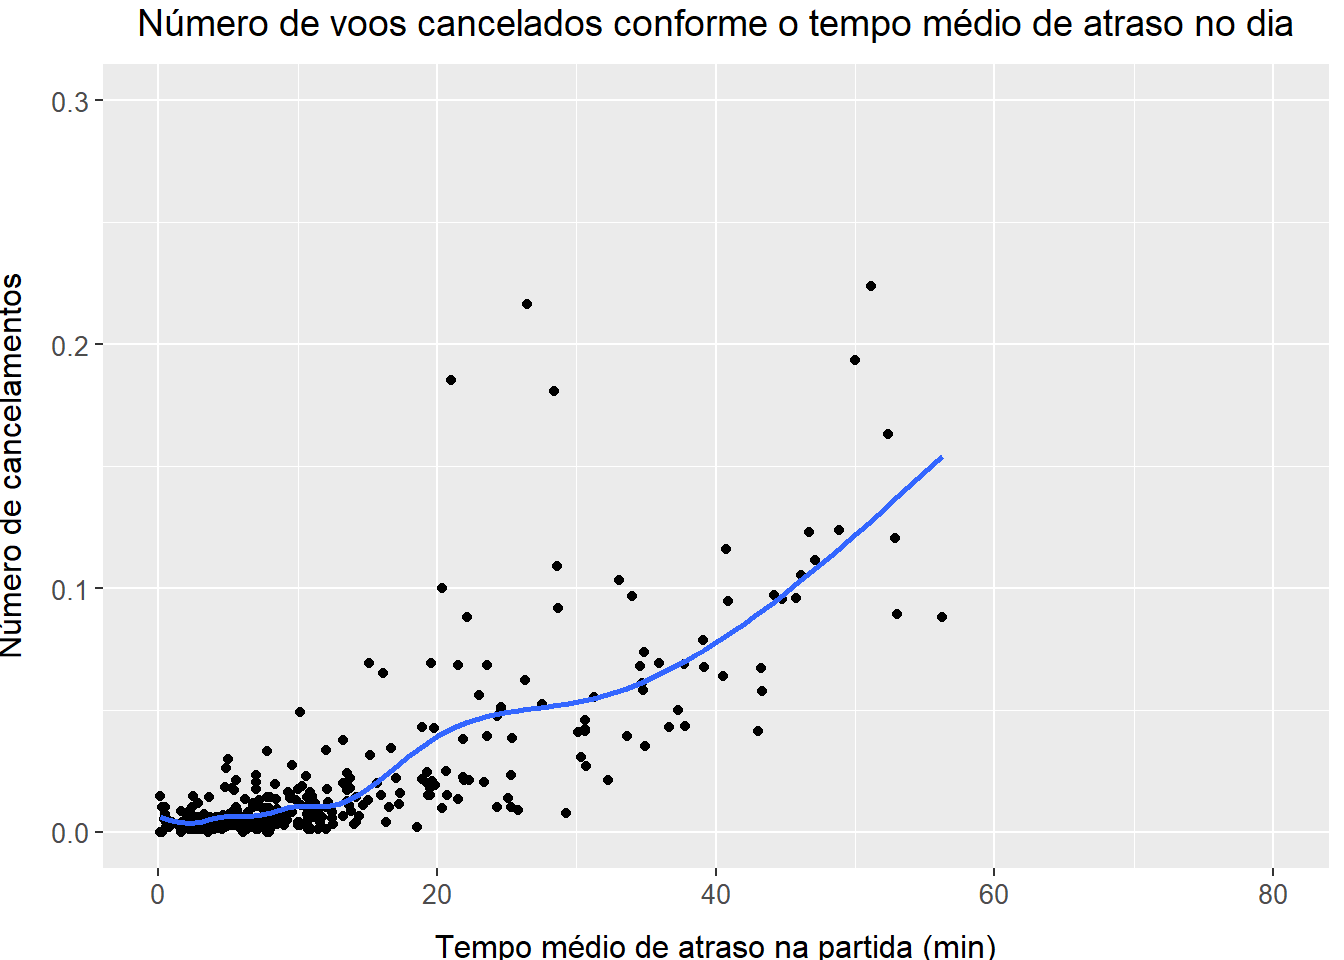
\includegraphics{r4ds_files/figure-latex/unnamed-chunk-67-1.pdf}

Parece existir uma relação entre o número de coos cancelados no dia e a média de atraso nos voos desse mesmo dia. Caso haja alguma condição desfavorável (tempo ruim, problemas na pista de decolagem/pouso, etc), o intervalo entre uma decolagem/pouso e outro pode aumentar significativamente gerando atrasos que se acumulam a ponto de alguns voos terem que ser cancelados (esse comportamento é real?).

\end{solution}

\hypertarget{exr3-7-5}{%
\subsection*{Exercício 3.7.5}\label{exr3-7-5}}
\addcontentsline{toc}{subsection}{Exercício 3.7.5}

Qual companhia tem os piores atrasos? Desafio: você consegue desembaralhar o efeito dos aeroportus ruins \emph{versus} companhiars ruins? Por quê/Por que não? ( Dica: pense em \texttt{flights\ \%\textgreater{}\%\ group\_by(cartier,\ dest)\ \%\textgreater{}\%\ summarize(n())})

\begin{solution}
Para verificar qual companhia tem os piores atrasos, vamos calcular o atraso médio por companhia.

\begin{Shaded}
\begin{Highlighting}[]
\NormalTok{flights }\SpecialCharTok{\%\textgreater{}\%} 
    \FunctionTok{group\_by}\NormalTok{(carrier) }\SpecialCharTok{\%\textgreater{}\%} 
    \FunctionTok{summarize}\NormalTok{(}
        \AttributeTok{mean\_delay =} \FunctionTok{mean}\NormalTok{(arr\_delay, }\AttributeTok{na.rm =} \ConstantTok{TRUE}\NormalTok{)}
\NormalTok{    ) }\SpecialCharTok{\%\textgreater{}\%}
    \FunctionTok{arrange}\NormalTok{(}\FunctionTok{desc}\NormalTok{(mean\_delay))}
\end{Highlighting}
\end{Shaded}

\begin{verbatim}
## # A tibble: 16 x 2
##    carrier mean_delay
##    <chr>        <dbl>
##  1 F9          21.9  
##  2 FL          20.1  
##  3 EV          15.8  
##  4 YV          15.6  
##  5 OO          11.9  
##  6 MQ          10.8  
##  7 WN           9.65 
##  8 B6           9.46 
##  9 9E           7.38 
## 10 UA           3.56 
## 11 US           2.13 
## 12 VX           1.76 
## 13 DL           1.64 
## 14 AA           0.364
## 15 HA          -6.92 
## 16 AS          -9.93
\end{verbatim}

Podemos notar que a companhia com o maior atraso médio é a F9 (Frontier Airlines Inc).

Para tentar desembaralhar o efeito de aeroportos ruins e companhias ruins, vamos:

\begin{itemize}
\tightlist
\item
  filtrar apenas os voos com atraso;
\item
  agrupar os voos conforme as rotas e companhias;
\item
  calcular o atraso médio e o total de voos por companhia no trecho (\texttt{arr\_delay} e \texttt{flights});
\item
  calcular o atraso médio e o total de voos do trecho de todas as companhias (\texttt{arr\_delay\_total} e \texttt{flights\_total});
\item
  calcular o atraso médio por voo da companhia (\texttt{arr\_delay\_mean\ \textless{}-\ arr\_delay\ /\ flights});
\item
  calcular o atraso ``médio'' das demais companhias (\texttt{arr\_delay\_others\ \textless{}-\ (arr\_delay\_total\ -\ arr\_delay)\ /\ (flights\_total\ -\ fligths)});
\item
  calcular a diferença entre o atraso médio da companhia e o atraso médio das outras companhias juntas (\texttt{arr\_delay\_diff\ \textless{}-\ arr\_delay\_mean\ -\ arr\_delay\_others});
\item
  remover valores cuja diferença não faça sentido (\texttt{is.finite(arr\_delay\_diff)});
\item
  agrupar por companhia;
\item
  calcular a média das diferenças de atraso da companhia (\texttt{arr\_delay\_diff});
\end{itemize}

\begin{Shaded}
\begin{Highlighting}[]
\NormalTok{(atrasos }\OtherTok{\textless{}{-}}\NormalTok{ flights }\SpecialCharTok{\%\textgreater{}\%} 
                \FunctionTok{filter}\NormalTok{(}\SpecialCharTok{!}\FunctionTok{is.na}\NormalTok{(arr\_delay)) }\SpecialCharTok{\%\textgreater{}\%}
                \FunctionTok{group\_by}\NormalTok{(origin, dest, carrier) }\SpecialCharTok{\%\textgreater{}\%}
                \FunctionTok{summarise}\NormalTok{(}
                    \AttributeTok{arr\_delay =} \FunctionTok{sum}\NormalTok{(arr\_delay),}
                    \AttributeTok{flights =} \FunctionTok{n}\NormalTok{()}
\NormalTok{                ) }\SpecialCharTok{\%\textgreater{}\%}
                \FunctionTok{group\_by}\NormalTok{(origin, dest) }\SpecialCharTok{\%\textgreater{}\%}
                \FunctionTok{mutate}\NormalTok{(}
                    \AttributeTok{arr\_delay\_total =} \FunctionTok{sum}\NormalTok{(arr\_delay),}
                    \AttributeTok{flights\_total =} \FunctionTok{sum}\NormalTok{(flights)}
\NormalTok{                ) }\SpecialCharTok{\%\textgreater{}\%}
                \FunctionTok{ungroup}\NormalTok{() }\SpecialCharTok{\%\textgreater{}\%}
                \FunctionTok{mutate}\NormalTok{(        }
                    \AttributeTok{arr\_delay\_mean =}\NormalTok{ arr\_delay }\SpecialCharTok{/}\NormalTok{ flights, }\CommentTok{\# atraso médio da companhia}
                    \AttributeTok{arr\_delay\_others =}\NormalTok{ (arr\_delay\_total }\SpecialCharTok{{-}}\NormalTok{ arr\_delay) }\SpecialCharTok{/}\NormalTok{ (flights\_total }\SpecialCharTok{{-}}\NormalTok{ flights), }\CommentTok{\# atraso médio das demais companhias}
                    \AttributeTok{arr\_delay\_diff =}\NormalTok{ arr\_delay\_mean }\SpecialCharTok{{-}}\NormalTok{ arr\_delay\_others }\CommentTok{\# diferença do atraso em relação às demais companhias}
\NormalTok{                ) }\SpecialCharTok{\%\textgreater{}\%}
                \FunctionTok{filter}\NormalTok{(}\FunctionTok{is.finite}\NormalTok{(arr\_delay\_diff)) }\SpecialCharTok{\%\textgreater{}\%}
                \FunctionTok{group\_by}\NormalTok{(carrier) }\SpecialCharTok{\%\textgreater{}\%}
                \FunctionTok{summarise}\NormalTok{(}
                    \AttributeTok{arr\_delay\_diff =} \FunctionTok{mean}\NormalTok{(arr\_delay\_diff)}
\NormalTok{                ) }\SpecialCharTok{\%\textgreater{}\%}
                \FunctionTok{arrange}\NormalTok{(}\FunctionTok{desc}\NormalTok{(arr\_delay\_diff)))}
\end{Highlighting}
\end{Shaded}

\begin{verbatim}
## `summarise()` has grouped output by 'origin', 'dest'. You can override using
## the `.groups` argument.
\end{verbatim}

\begin{verbatim}
## # A tibble: 15 x 2
##    carrier arr_delay_diff
##    <chr>            <dbl>
##  1 OO              27.3  
##  2 F9              17.3  
##  3 EV              11.0  
##  4 B6               6.41 
##  5 FL               2.57 
##  6 VX              -0.202
##  7 AA              -0.970
##  8 WN              -1.27 
##  9 UA              -1.86 
## 10 MQ              -2.48 
## 11 YV              -2.81 
## 12 9E              -3.54 
## 13 US              -4.14 
## 14 DL             -10.2  
## 15 AS             -15.8
\end{verbatim}

Desconsiderando o efeito de trechos e aeroportos ruins, a companhia com maior atraso é a OO (SkyWest Airlines Inc.).

\begin{Shaded}
\begin{Highlighting}[]
\NormalTok{atrasos }\SpecialCharTok{\%\textgreater{}\%}
    \FunctionTok{left\_join}\NormalTok{(airlines, }\AttributeTok{by =} \StringTok{"carrier"}\NormalTok{) }\SpecialCharTok{\%\textgreater{}\%}
    \FunctionTok{ggplot}\NormalTok{(}\FunctionTok{aes}\NormalTok{(}
\NormalTok{        arr\_delay\_diff, }
        \FunctionTok{reorder}\NormalTok{(name, }\FunctionTok{desc}\NormalTok{(arr\_delay\_diff))}
\NormalTok{    )) }\SpecialCharTok{+}
        \FunctionTok{geom\_col}\NormalTok{() }\SpecialCharTok{+}
        \FunctionTok{labs}\NormalTok{(}
            \AttributeTok{title =} \StringTok{"Atrasos por companhia aérea"}\NormalTok{,}
            \AttributeTok{y =} \StringTok{"Companhia aérea"}\NormalTok{,}
            \AttributeTok{x =} \StringTok{"Tempo médio de atraso (em min.)"}
\NormalTok{        ) }\SpecialCharTok{+}
\NormalTok{        tema}
\end{Highlighting}
\end{Shaded}

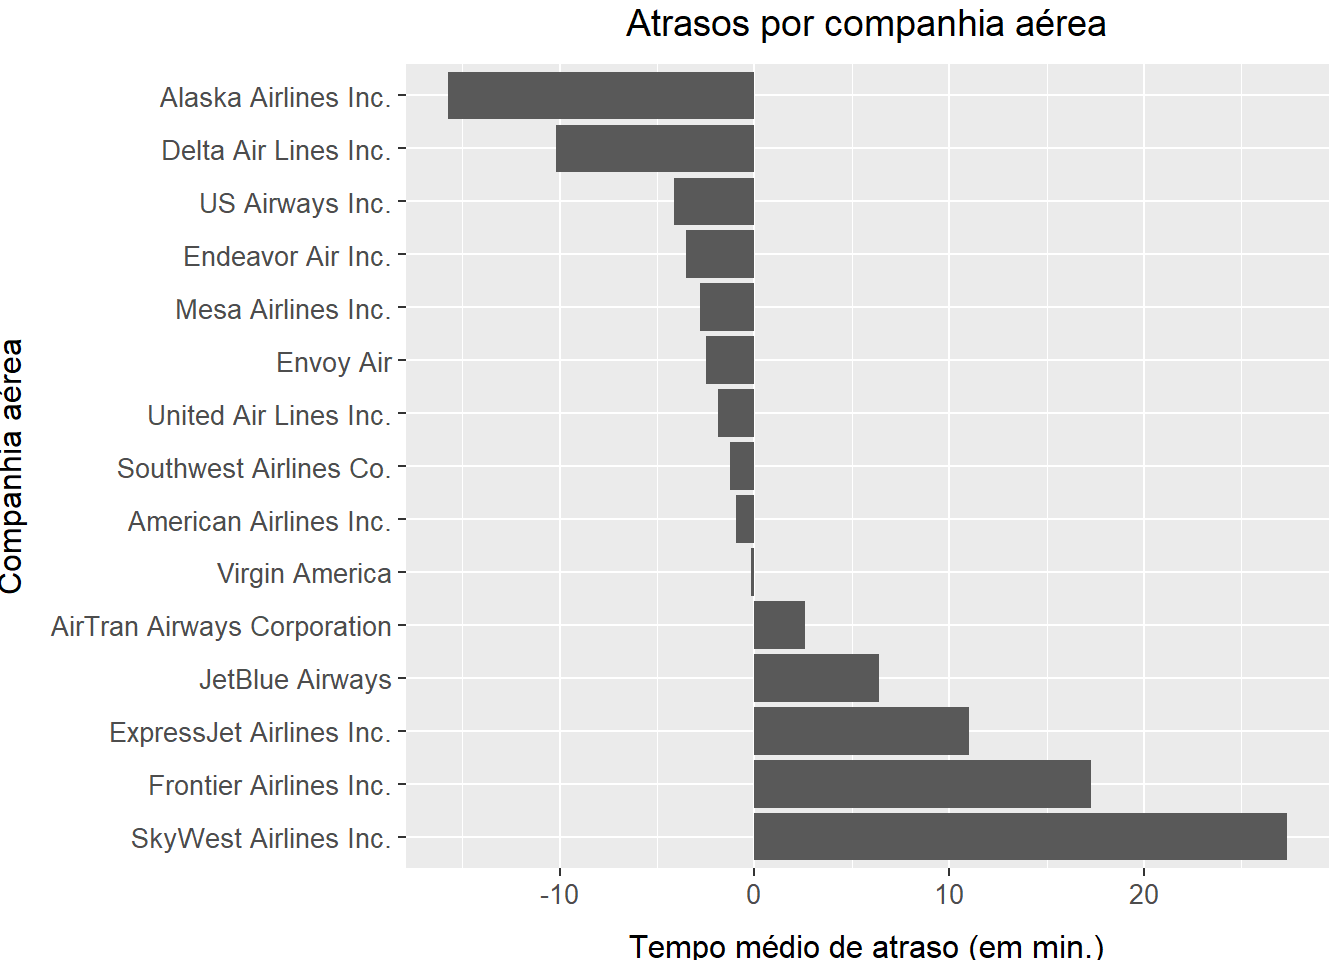
\includegraphics{r4ds_files/figure-latex/unnamed-chunk-70-1.pdf}
\end{solution}

\hypertarget{exr3-7-6}{%
\subsection*{Exercício 3.7.6}\label{exr3-7-6}}
\addcontentsline{toc}{subsection}{Exercício 3.7.6}

Para cada avião, conte o número de voos antes do primeiro atraso de mais de uma hora.

\begin{solution}

Utilizando a variável \texttt{flight} para identificar o voo e a variável \texttt{arr\_delay} como parâmetro para determinar o tempo de atraso:

\begin{itemize}
\tightlist
\item
  ordenamos o data-frame conforme a hora agendada para decolagem;
\item
  agrupamos pelo número do voo;
\item
  utilizamos as funções \texttt{first()} e \texttt{which()} para buscar a posição do primeiro elemento que é \texttt{NA} ou o atraso é maior do que 60 min.
\end{itemize}

Obs.: \texttt{NA} indica que aquele voo não teve nenhum atraso superior a 60 min.

\begin{Shaded}
\begin{Highlighting}[]
\NormalTok{flights }\SpecialCharTok{\%\textgreater{}\%}
    \FunctionTok{arrange}\NormalTok{(time\_hour) }\SpecialCharTok{\%\textgreater{}\%}    
    \FunctionTok{group\_by}\NormalTok{(flight) }\SpecialCharTok{\%\textgreater{}\%}
    \FunctionTok{summarise}\NormalTok{(}
        \AttributeTok{first\_delay\_pos =} \FunctionTok{first}\NormalTok{(}\FunctionTok{which}\NormalTok{(}\FunctionTok{is.na}\NormalTok{(arr\_delay) }\SpecialCharTok{|}\NormalTok{ arr\_delay }\SpecialCharTok{\textgreater{}} \DecValTok{60}\NormalTok{)) }\SpecialCharTok{{-}} \DecValTok{1}
\NormalTok{    )}
\end{Highlighting}
\end{Shaded}

\begin{verbatim}
## # A tibble: 3,844 x 2
##    flight first_delay_pos
##     <int>           <dbl>
##  1      1              47
##  2      2              NA
##  3      3               9
##  4      4              77
##  5      5              11
##  6      6              23
##  7      7              17
##  8      8              15
##  9      9              12
## 10     10              24
## # i 3,834 more rows
\end{verbatim}

\end{solution}

\hypertarget{exr3-7-7}{%
\subsection*{Exercício 3.7.7}\label{exr3-7-7}}
\addcontentsline{toc}{subsection}{Exercício 3.7.7}

O que o argumento \texttt{sort} para \texttt{count()} faz? Quando você pode usá-lo?

\begin{solution}
Utilizando o comando \texttt{?count}, identificamos que o argumento \texttt{sort} organiza a contagem em ordem decrescente.
\end{solution}

\hypertarget{mudanuxe7as-agrupadas-e-filtros}{%
\section{Mudanças agrupadas (e filtros)}\label{mudanuxe7as-agrupadas-e-filtros}}

\hypertarget{exr3-8-1}{%
\subsection*{Exercício 3.8.1}\label{exr3-8-1}}
\addcontentsline{toc}{subsection}{Exercício 3.8.1}

Volte à tabela de funções de mudança e filtragem úteis. Descreva como cada operaçõa muda quando você as combina com o agrupamento.

\begin{solution}
x
\end{solution}

\hypertarget{exr3-8-2}{%
\subsection*{Exercício 3.8.2}\label{exr3-8-2}}
\addcontentsline{toc}{subsection}{Exercício 3.8.2}

Qual avião (\texttt{tailnum}) tem o pior registro de pontualidade?

\begin{solution}
Vamos inicialmente considerar que um voo é pontual se o tempo de atraso na chegada (\texttt{arr\_delay}) é igual ou inferior a zero e, para considerar um avião como mais ou menos pontual, levaremos em consideração a proporção de voos pontuais que ele realizou.

\begin{Shaded}
\begin{Highlighting}[]
\NormalTok{flights }\SpecialCharTok{\%\textgreater{}\%}
    \CommentTok{\# Considerar apenas os registros que tem a informação sobre o avião, }
    \CommentTok{\# hora de chegada e atraso na chegada}
    \FunctionTok{filter}\NormalTok{(}\SpecialCharTok{!}\FunctionTok{is.na}\NormalTok{(tailnum), }\SpecialCharTok{!}\FunctionTok{is.na}\NormalTok{(arr\_time), }\SpecialCharTok{!}\FunctionTok{is.na}\NormalTok{(arr\_delay)) }\SpecialCharTok{\%\textgreater{}\%}
    \CommentTok{\# Criar uma variável booleana (0 ou 1) que indica se o voo foi pontual}
    \FunctionTok{mutate}\NormalTok{(}
        \AttributeTok{on\_time =} \SpecialCharTok{!}\FunctionTok{is.na}\NormalTok{(arr\_time) }\SpecialCharTok{\&}\NormalTok{ arr\_delay }\SpecialCharTok{\textless{}=} \DecValTok{0}
\NormalTok{    ) }\SpecialCharTok{\%\textgreater{}\%}
    \CommentTok{\# Calcular a proporção de voos pontuais e o número de voos por avião}
    \FunctionTok{group\_by}\NormalTok{(tailnum) }\SpecialCharTok{\%\textgreater{}\%}
    \FunctionTok{summarise}\NormalTok{(}
        \AttributeTok{n =} \FunctionTok{n}\NormalTok{(),}
        \AttributeTok{arr\_delay =} \FunctionTok{mean}\NormalTok{(arr\_delay),}
        \AttributeTok{on\_time =} \FunctionTok{mean}\NormalTok{(on\_time)}
\NormalTok{    ) }\SpecialCharTok{\%\textgreater{}\%}
    \CommentTok{\# Descartar aviões que voaram 20 vezes ou menos}
    \FunctionTok{filter}\NormalTok{(n }\SpecialCharTok{\textgreater{}} \DecValTok{20}\NormalTok{) }\SpecialCharTok{\%\textgreater{}\%}
    \CommentTok{\# Ordenar por percentiual de voos pontuais}
    \FunctionTok{arrange}\NormalTok{(}\FunctionTok{desc}\NormalTok{(on\_time)) }\SpecialCharTok{\%\textgreater{}\%}
    \FunctionTok{head}\NormalTok{()}
\end{Highlighting}
\end{Shaded}

\begin{verbatim}
## # A tibble: 6 x 4
##   tailnum     n arr_delay on_time
##   <chr>   <int>     <dbl>   <dbl>
## 1 N382HA     26    -23.5    0.885
## 2 N553AA     51     -6.33   0.863
## 3 N423AS     29    -22.3    0.862
## 4 N538AA     35     -9.6    0.857
## 5 N548AA     49    -15.5    0.857
## 6 N5EJAA     21    -12.5    0.857
\end{verbatim}

Com base na configuração acima, o avião N382HA é o mais pontual, com 88,46\% dos 26 voos sendo executados com pontualidade.
\end{solution}

\hypertarget{exr3-8-3}{%
\subsection*{Exercício 3.8.3}\label{exr3-8-3}}
\addcontentsline{toc}{subsection}{Exercício 3.8.3}

A que horas você deverá voar se quiser evitar atrasos ao máximo.

\begin{solution}

O problema depende de encontrar o horário em que ocorrem menos atrasos. Consideraremos a hora inteira como parâmetro para a busca (\texttt{hour}) e utilizaremos a média dos tempos de atraso dos voos.

\begin{Shaded}
\begin{Highlighting}[]
\NormalTok{flights }\SpecialCharTok{\%\textgreater{}\%}
    \FunctionTok{filter}\NormalTok{(}\SpecialCharTok{!}\FunctionTok{is.na}\NormalTok{(hour)) }\SpecialCharTok{\%\textgreater{}\%}
    \FunctionTok{group\_by}\NormalTok{(hour) }\SpecialCharTok{\%\textgreater{}\%}
    \FunctionTok{summarise}\NormalTok{(}
        \AttributeTok{arr\_delay =} \FunctionTok{mean}\NormalTok{(arr\_delay, }\AttributeTok{na.rm =}\NormalTok{ T)}
\NormalTok{    ) }\SpecialCharTok{\%\textgreater{}\%}
    \FunctionTok{arrange}\NormalTok{(arr\_delay) }\SpecialCharTok{\%\textgreater{}\%}
    \FunctionTok{head}\NormalTok{()}
\end{Highlighting}
\end{Shaded}

\begin{verbatim}
## # A tibble: 6 x 2
##    hour arr_delay
##   <dbl>     <dbl>
## 1     7    -5.30 
## 2     5    -4.80 
## 3     6    -3.38 
## 4     9    -1.45 
## 5     8    -1.11 
## 6    10     0.954
\end{verbatim}

\end{solution}

\hypertarget{exr3-8-4}{%
\subsection*{Exercício 3.8.4}\label{exr3-8-4}}
\addcontentsline{toc}{subsection}{Exercício 3.8.4}

Para cada destino, calcule os minutos totais de atraso. Para cada voo, calcule a proporção de atraso total par seu destino.

\begin{solution}

R.: Para calcular o atraso total (em minutos) por destino, somaremos os valores da variável \texttt{arr\_delay} de todos os voos para cada destino (\texttt{group\_by(dest)}). Em seguida, para calcular a proporção com a qual cada voo colabora para o atraso total do destino, utilizaremos a razão entre o atraso do voo e o total do grupo ao qual pertence.

\begin{Shaded}
\begin{Highlighting}[]
\NormalTok{flights }\SpecialCharTok{\%\textgreater{}\%}
    \FunctionTok{filter}\NormalTok{(arr\_delay }\SpecialCharTok{\textgreater{}} \DecValTok{0}\NormalTok{) }\SpecialCharTok{\%\textgreater{}\%}
    \FunctionTok{group\_by}\NormalTok{(dest) }\SpecialCharTok{\%\textgreater{}\%}
    \FunctionTok{mutate}\NormalTok{(}
        \AttributeTok{arr\_delay\_total =} \FunctionTok{sum}\NormalTok{(arr\_delay),}
        \AttributeTok{arr\_delay\_prop =}\NormalTok{ arr\_delay }\SpecialCharTok{/}\NormalTok{ arr\_delay\_total}
\NormalTok{    ) }\SpecialCharTok{\%\textgreater{}\%}
    \FunctionTok{select}\NormalTok{ (dest, flight, dep\_time, arr\_delay, arr\_delay\_total, arr\_delay\_prop) }\SpecialCharTok{\%\textgreater{}\%}
    \FunctionTok{arrange}\NormalTok{(dest, }\FunctionTok{desc}\NormalTok{(arr\_delay\_prop)) }\SpecialCharTok{\%\textgreater{}\%}
    \FunctionTok{head}\NormalTok{()}
\end{Highlighting}
\end{Shaded}

\begin{verbatim}
## # A tibble: 6 x 6
## # Groups:   dest [1]
##   dest  flight dep_time arr_delay arr_delay_total arr_delay_prop
##   <chr>  <int>    <int>     <dbl>           <dbl>          <dbl>
## 1 ABQ     1505     2145       153            4487         0.0341
## 2 ABQ       65     2223       149            4487         0.0332
## 3 ABQ       65     2146       138            4487         0.0308
## 4 ABQ     1505     2206       137            4487         0.0305
## 5 ABQ       65     2220       136            4487         0.0303
## 6 ABQ     1505     2025       126            4487         0.0281
\end{verbatim}

\end{solution}

\hypertarget{exr3-8-5}{%
\subsection*{Exercício 3.8.5}\label{exr3-8-5}}
\addcontentsline{toc}{subsection}{Exercício 3.8.5}

Atrasos são normalmente temporariamente correlacionados: mesmo quando o problema que causou o atraso inicial foi resolvido, , voos posteriores atrasam para permitir que os voos anteriores decolem. Usando \texttt{lag()}, explore como o atraso de um voo está relacionado com o atraso imediatamente anterior.

\begin{solution}
Considerando o atraso na decolagem, vamos inicialmente ordenar os voos por aeroporto, data e hora da decolagem. Em seguida, agrupando pelo aeroporto, coletamos o atraso do voo anteriot (note que o \texttt{mutate} irá atuar sobre o grupo apenas. Não faz sentido considerar o voo anterior em outro aeroporto!). Na sequência, podemos agrupar pelo tempo de atraso do voo anterior para calcular a média dos atrasos dos voos. Por fim, é exibido o gráfico.

Avaliando a imagem, podemos notar a tendência de que, quanto maior o atraso do voo imediatamente anterior, maior será o atraso do voo atual. O padrão crescente segue até atrasos de aproximadamente 435 minutos. Depois passa a decrescer, o que deve ser analisado mais aprofundadamente.

\begin{Shaded}
\begin{Highlighting}[]
\NormalTok{flights }\SpecialCharTok{\%\textgreater{}\%}
    \FunctionTok{arrange}\NormalTok{(origin, month, day, dep\_time) }\SpecialCharTok{\%\textgreater{}\%}
    \FunctionTok{group\_by}\NormalTok{(origin) }\SpecialCharTok{\%\textgreater{}\%}
    \FunctionTok{mutate}\NormalTok{(}\AttributeTok{prev\_dep\_delay =} \FunctionTok{lag}\NormalTok{(dep\_delay)) }\SpecialCharTok{\%\textgreater{}\%}
    \FunctionTok{filter}\NormalTok{(}\SpecialCharTok{!}\FunctionTok{is.na}\NormalTok{(dep\_delay), }\SpecialCharTok{!}\FunctionTok{is.na}\NormalTok{(prev\_dep\_delay)) }\SpecialCharTok{\%\textgreater{}\%}
    \FunctionTok{group\_by}\NormalTok{(origin, prev\_dep\_delay) }\SpecialCharTok{\%\textgreater{}\%}
    \FunctionTok{summarise}\NormalTok{(}\AttributeTok{dep\_delay\_mean =} \FunctionTok{mean}\NormalTok{(dep\_delay)) }\SpecialCharTok{\%\textgreater{}\%}
    \FunctionTok{ggplot}\NormalTok{(}\FunctionTok{aes}\NormalTok{(prev\_dep\_delay, dep\_delay\_mean)) }\SpecialCharTok{+}
        \FunctionTok{geom\_point}\NormalTok{() }\SpecialCharTok{+}
        \FunctionTok{geom\_smooth}\NormalTok{(}\AttributeTok{se =} \ConstantTok{FALSE}\NormalTok{) }\SpecialCharTok{+}        
        \FunctionTok{scale\_x\_continuous}\NormalTok{(}\AttributeTok{breaks =} \FunctionTok{seq}\NormalTok{(}\DecValTok{0}\NormalTok{, }\DecValTok{1300}\NormalTok{, }\AttributeTok{by =} \DecValTok{60}\NormalTok{)) }\SpecialCharTok{+}
        \FunctionTok{scale\_y\_continuous}\NormalTok{(}\AttributeTok{breaks =} \FunctionTok{seq}\NormalTok{(}\DecValTok{0}\NormalTok{, }\DecValTok{450}\NormalTok{, }\AttributeTok{by =} \DecValTok{60}\NormalTok{)) }\SpecialCharTok{+}
        \FunctionTok{labs}\NormalTok{(}
            \AttributeTok{title =} \StringTok{"Atraso médio na decolagem em função do atraso na decolagem anterior."}\NormalTok{,}
            \AttributeTok{x =} \StringTok{"Atraso na decolagem anterior (min.)"}\NormalTok{,}
            \AttributeTok{y =} \StringTok{"Atraso médio na decolagem (min.)"}
\NormalTok{        ) }\SpecialCharTok{+}
\NormalTok{        tema}
\end{Highlighting}
\end{Shaded}

\begin{verbatim}
## `summarise()` has grouped output by 'origin'. You can override using the
## `.groups` argument.
## `geom_smooth()` using method = 'gam' and formula = 'y ~ s(x, bs = "cs")'
\end{verbatim}

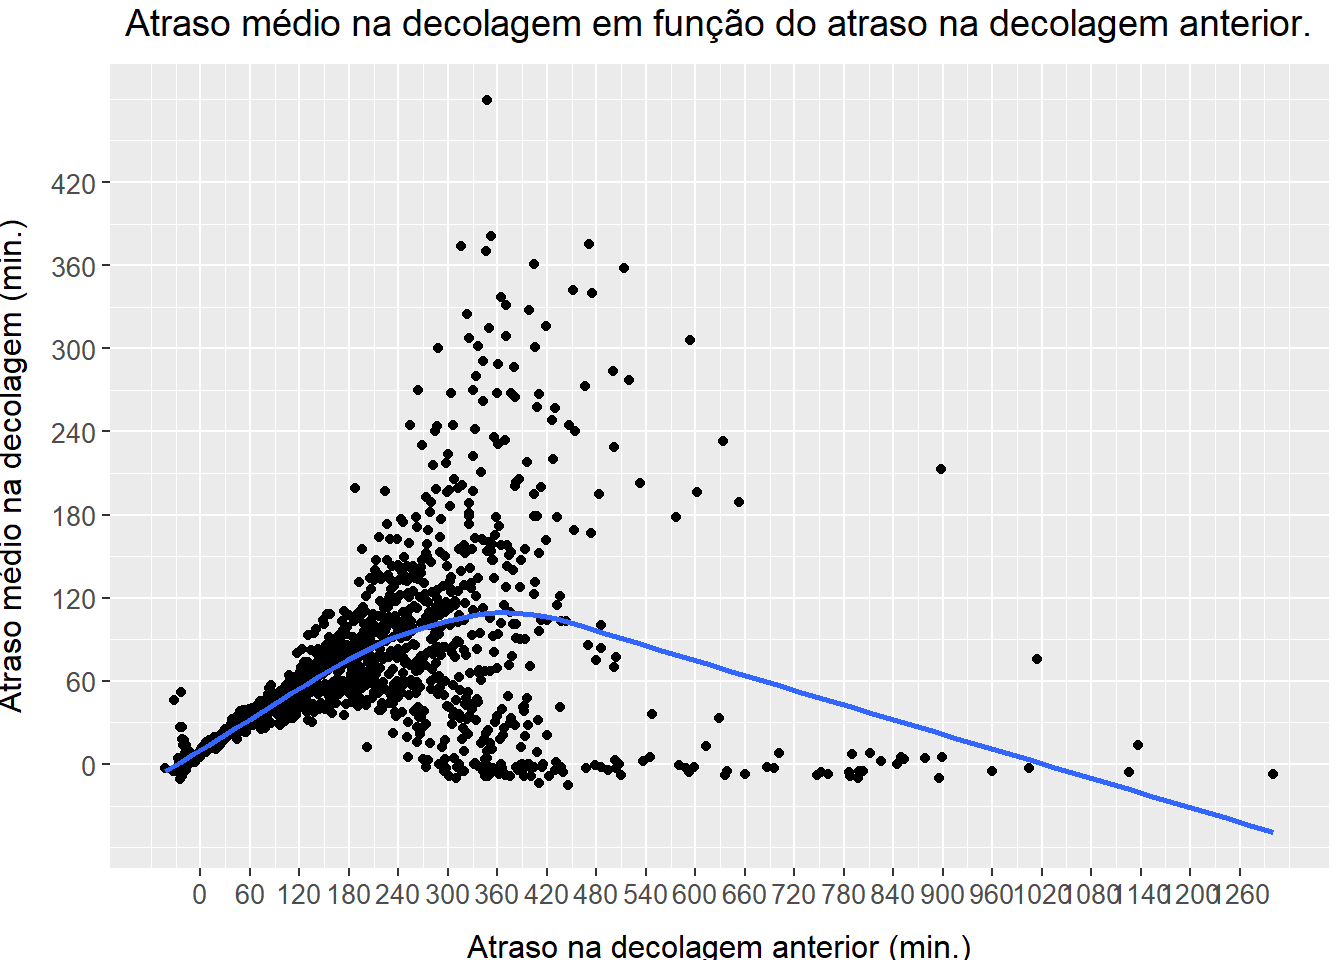
\includegraphics{r4ds_files/figure-latex/unnamed-chunk-75-1.pdf}

É importante notar que o padrão se repete se avaliarmos cada aeroporto individualmente.

\begin{Shaded}
\begin{Highlighting}[]
\NormalTok{flights }\SpecialCharTok{\%\textgreater{}\%}
    \FunctionTok{arrange}\NormalTok{(origin, month, day, dep\_time) }\SpecialCharTok{\%\textgreater{}\%}
    \FunctionTok{group\_by}\NormalTok{(origin) }\SpecialCharTok{\%\textgreater{}\%}
    \FunctionTok{mutate}\NormalTok{(}\AttributeTok{prev\_dep\_delay =} \FunctionTok{lag}\NormalTok{(dep\_delay)) }\SpecialCharTok{\%\textgreater{}\%}
    \FunctionTok{filter}\NormalTok{(}\SpecialCharTok{!}\FunctionTok{is.na}\NormalTok{(dep\_delay), }\SpecialCharTok{!}\FunctionTok{is.na}\NormalTok{(prev\_dep\_delay)) }\SpecialCharTok{\%\textgreater{}\%}
    \FunctionTok{group\_by}\NormalTok{(origin, prev\_dep\_delay) }\SpecialCharTok{\%\textgreater{}\%}
    \FunctionTok{summarise}\NormalTok{(}\AttributeTok{dep\_delay\_mean =} \FunctionTok{mean}\NormalTok{(dep\_delay)) }\SpecialCharTok{\%\textgreater{}\%}
    \FunctionTok{ggplot}\NormalTok{(}\FunctionTok{aes}\NormalTok{(prev\_dep\_delay, dep\_delay\_mean)) }\SpecialCharTok{+}
        \FunctionTok{geom\_point}\NormalTok{() }\SpecialCharTok{+}
        \FunctionTok{geom\_smooth}\NormalTok{(}\AttributeTok{se =} \ConstantTok{FALSE}\NormalTok{) }\SpecialCharTok{+}
        \FunctionTok{facet\_wrap}\NormalTok{(}\SpecialCharTok{\textasciitilde{}}\NormalTok{ origin, }\AttributeTok{ncol =} \DecValTok{1}\NormalTok{) }\SpecialCharTok{+}
        \FunctionTok{scale\_x\_continuous}\NormalTok{(}\AttributeTok{breaks =} \FunctionTok{seq}\NormalTok{(}\DecValTok{0}\NormalTok{, }\DecValTok{1300}\NormalTok{, }\AttributeTok{by =} \DecValTok{60}\NormalTok{)) }\SpecialCharTok{+}
        \FunctionTok{scale\_y\_continuous}\NormalTok{(}\AttributeTok{breaks =} \FunctionTok{seq}\NormalTok{(}\DecValTok{0}\NormalTok{, }\DecValTok{450}\NormalTok{, }\AttributeTok{by =} \DecValTok{60}\NormalTok{)) }\SpecialCharTok{+}
        \FunctionTok{labs}\NormalTok{(}
            \AttributeTok{title =} \StringTok{"Atraso médio na decolagem em função do atraso na decolagem anterior."}\NormalTok{,}
            \AttributeTok{x =} \StringTok{"Atraso na decolagem anterior (min.)"}\NormalTok{,}
            \AttributeTok{y =} \StringTok{"Atraso médio na decolagem (min.)"}
\NormalTok{        ) }\SpecialCharTok{+}
\NormalTok{        tema}
\end{Highlighting}
\end{Shaded}

\begin{verbatim}
## `summarise()` has grouped output by 'origin'. You can override using the
## `.groups` argument.
## `geom_smooth()` using method = 'loess' and formula = 'y ~ x'
\end{verbatim}

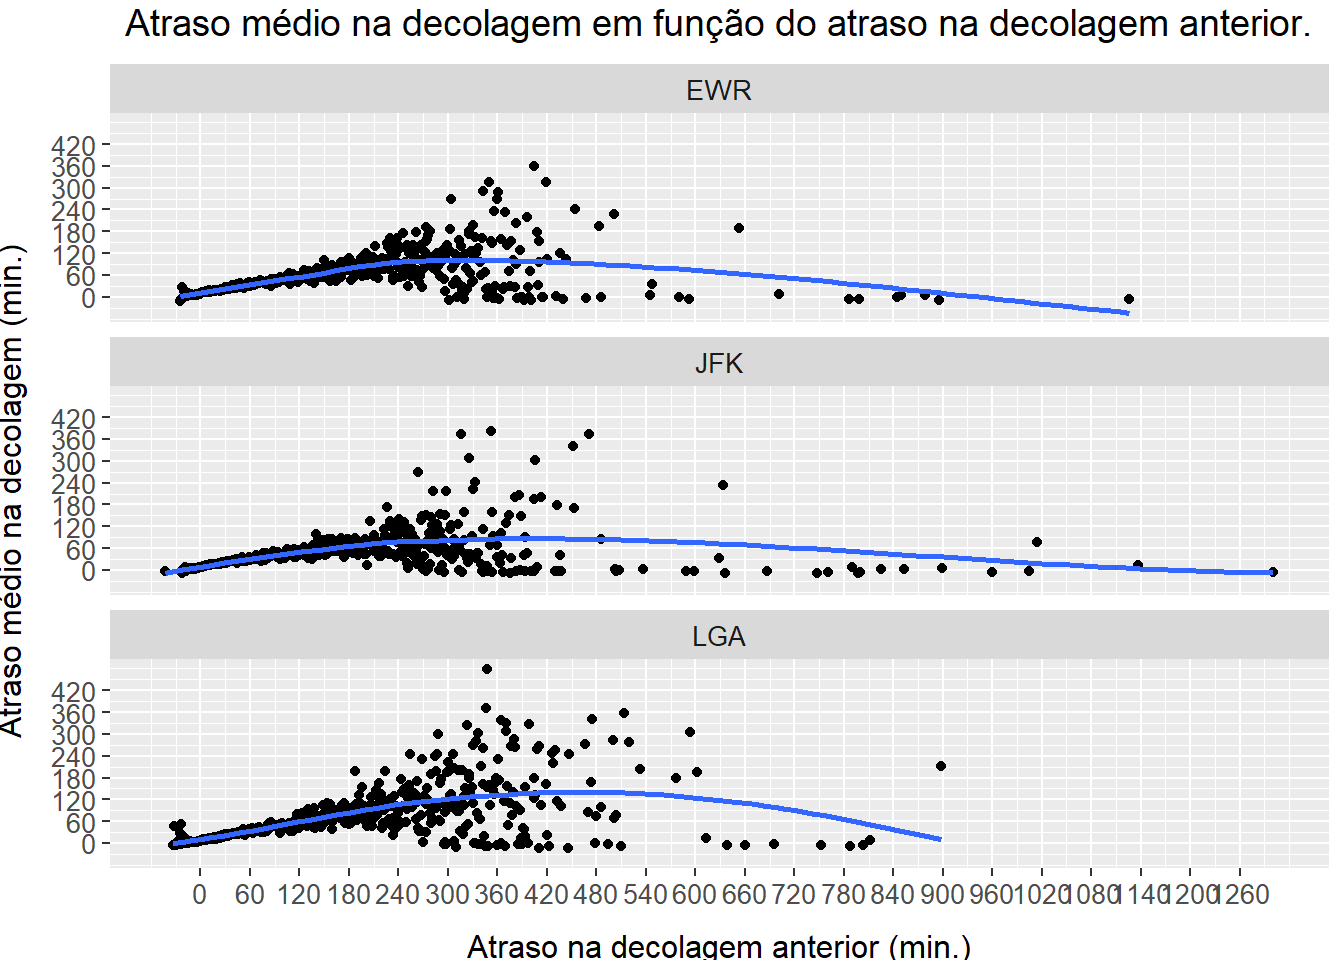
\includegraphics{r4ds_files/figure-latex/unnamed-chunk-76-1.pdf}
\end{solution}

\hypertarget{exr3-8-6}{%
\subsection*{Exercício 3.8.6}\label{exr3-8-6}}
\addcontentsline{toc}{subsection}{Exercício 3.8.6}

Veja cada destino. Você consegue encontrar os voos que são suspeitamente rápidos? (Ou seja, voos que representam um erro de entrada de dados em potencial). Calcule o tempo de viagem de um voo relativo ao voo mais curto para aquele destino. Quais voos ficaram mais atrasados no ar?

\begin{solution}
Inicialmente calcularemos a média e o desvio padrão para cada rota (\texttt{origin}, \texttt{dest}) e, na sequência, calcularemos o \emph{z-score} para avaliar a distribuição dos tempos de voo. Usaremos a mediana e o intervalo interquartílico para escapar do efeito de outliers.

\begin{Shaded}
\begin{Highlighting}[]
\NormalTok{standardized }\OtherTok{\textless{}{-}}\NormalTok{ flights }\SpecialCharTok{\%\textgreater{}\%}
    \FunctionTok{filter}\NormalTok{(}\SpecialCharTok{!}\FunctionTok{is.na}\NormalTok{(air\_time)) }\SpecialCharTok{\%\textgreater{}\%}            \CommentTok{\# Remover os voos sem informação do tempo de voo}
    \FunctionTok{group\_by}\NormalTok{(origin, dest) }\SpecialCharTok{\%\textgreater{}\%}              \CommentTok{\# Agrupar pela rota (origin {-}\textgreater{} dest)}
    \FunctionTok{mutate}\NormalTok{(}
        \AttributeTok{median =} \FunctionTok{median}\NormalTok{(air\_time),          }\CommentTok{\# Calcular a média de cada grupo}
        \AttributeTok{iqr =} \FunctionTok{IQR}\NormalTok{(air\_time),                }\CommentTok{\# Calcular o desvio padrão do grupo}
        \AttributeTok{n =} \FunctionTok{n}\NormalTok{(),                            }\CommentTok{\# Calcular o tamanho do grupo}
        \AttributeTok{z =}\NormalTok{ (air\_time }\SpecialCharTok{{-}}\NormalTok{ median) }\SpecialCharTok{/}\NormalTok{ iqr       }\CommentTok{\# Calcular o z{-}score de cada voo dentro do grupo}
\NormalTok{    ) }\SpecialCharTok{\%\textgreater{}\%}
    \FunctionTok{ungroup}\NormalTok{()}

\NormalTok{standardized }\SpecialCharTok{\%\textgreater{}\%}    
    \FunctionTok{ggplot}\NormalTok{(}\FunctionTok{aes}\NormalTok{(}\AttributeTok{x =}\NormalTok{ z)) }\SpecialCharTok{+}
        \FunctionTok{geom\_density}\NormalTok{() }\SpecialCharTok{+}
        \FunctionTok{geom\_vline}\NormalTok{(}\FunctionTok{aes}\NormalTok{(}\AttributeTok{xintercept =} \SpecialCharTok{{-}}\FloatTok{2.5}\NormalTok{), }\AttributeTok{linetype =} \StringTok{"dashed"}\NormalTok{) }\SpecialCharTok{+}
        \FunctionTok{geom\_vline}\NormalTok{(}\FunctionTok{aes}\NormalTok{(}\AttributeTok{xintercept =} \FloatTok{2.5}\NormalTok{), }\AttributeTok{linetype =} \StringTok{"dashed"}\NormalTok{) }\SpecialCharTok{+}
        \FunctionTok{scale\_x\_continuous}\NormalTok{(}\AttributeTok{breaks =} \FunctionTok{seq}\NormalTok{(}\SpecialCharTok{{-}}\DecValTok{10}\NormalTok{, }\DecValTok{30}\NormalTok{, }\AttributeTok{by =} \DecValTok{1}\NormalTok{)) }\SpecialCharTok{+}
\NormalTok{        tema}
\end{Highlighting}
\end{Shaded}

\begin{verbatim}
## Warning: Removed 4 rows containing non-finite values (`stat_density()`).
\end{verbatim}

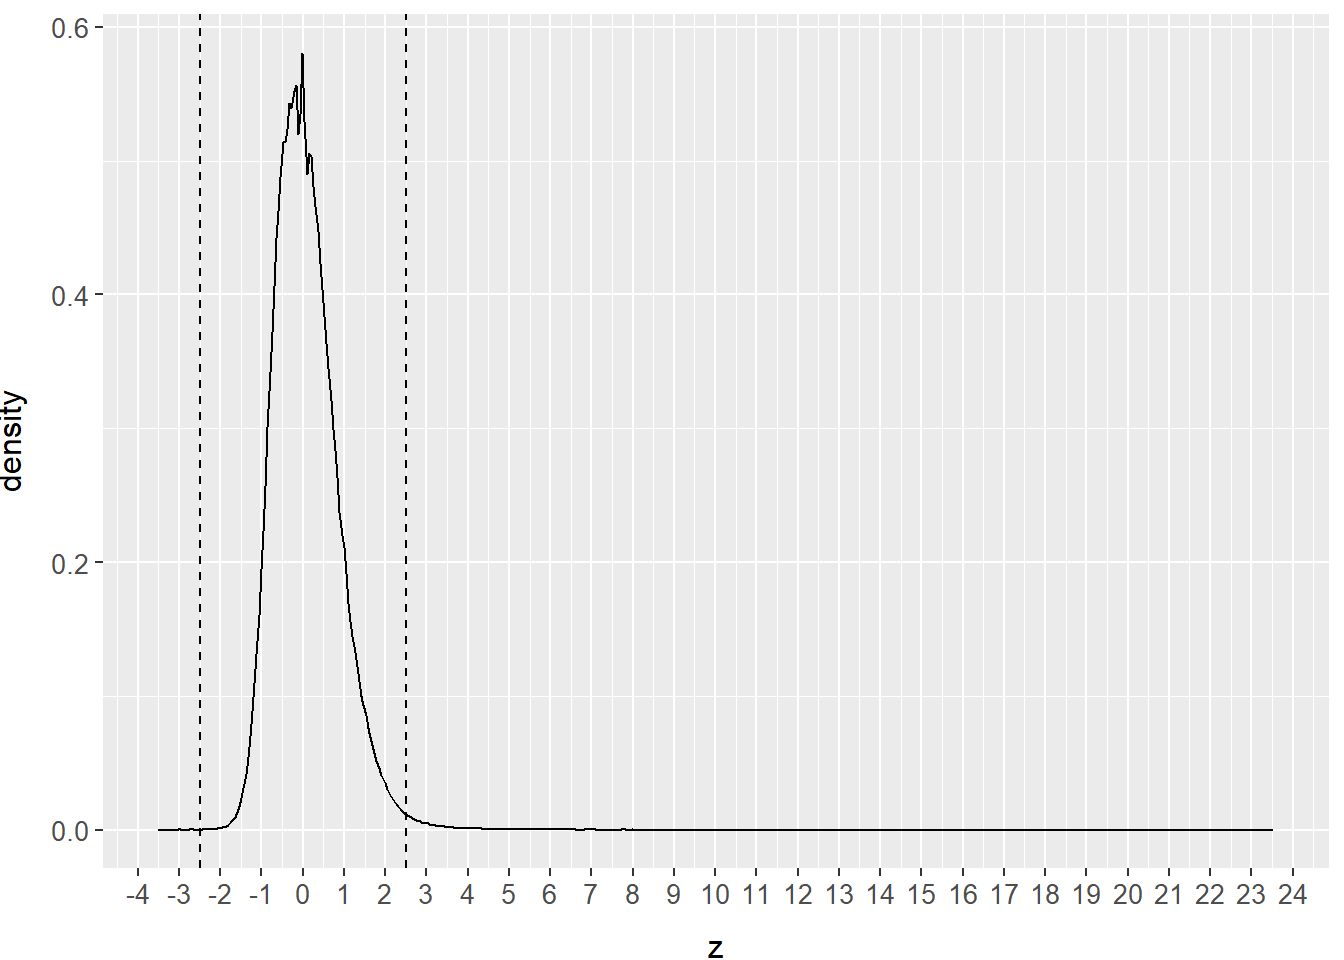
\includegraphics{r4ds_files/figure-latex/unnamed-chunk-77-1.pdf}

Os voos com \emph{z-score} muito baixo, são aqueles cujo tempo de voo foi muito menor do que a média, ou seja, os mais rápidos.

\begin{Shaded}
\begin{Highlighting}[]
\NormalTok{standardized }\SpecialCharTok{\%\textgreater{}\%}
    \FunctionTok{arrange}\NormalTok{(z) }\SpecialCharTok{\%\textgreater{}\%}
    \FunctionTok{select}\NormalTok{(carrier, flight, origin, dest, month, day, air\_time, median, iqr, z) }\SpecialCharTok{\%\textgreater{}\%}
    \FunctionTok{head}\NormalTok{(}\DecValTok{10}\NormalTok{)}
\end{Highlighting}
\end{Shaded}

\begin{verbatim}
## # A tibble: 10 x 10
##    carrier flight origin dest  month   day air_time median   iqr     z
##    <chr>    <int> <chr>  <chr> <int> <int>    <dbl>  <dbl> <dbl> <dbl>
##  1 EV        4667 EWR    MSP       7     2       93    149    16 -3.5 
##  2 DL        1499 LGA    ATL       5    25       65    112    14 -3.36
##  3 US        2132 LGA    BOS       3     2       21     37     5 -3.2 
##  4 B6          30 JFK    ROC       3    25       35     51     5 -3.2 
##  5 B6        2002 JFK    BUF      11    10       38     57     6 -3.17
##  6 EV        4292 EWR    GSP       5    13       55     92    12 -3.08
##  7 EV        4249 EWR    SYR       3    15       30     39     3 -3   
##  8 EV        4580 EWR    BTV       6    29       34     46     4 -3   
##  9 EV        3830 EWR    RIC       7     2       35     53     6 -3   
## 10 EV        4687 EWR    CVG       9    29       62     95    11 -3
\end{verbatim}

Adicionalmente, vamos considerar também a velocidade do voo (\texttt{mph\ \textless{}-\ distance\ /\ (air\_time\ /\ 60)}).

\begin{Shaded}
\begin{Highlighting}[]
\NormalTok{standardized }\SpecialCharTok{\%\textgreater{}\%}
    \FunctionTok{mutate}\NormalTok{(}
        \AttributeTok{mph =}\NormalTok{ distance }\SpecialCharTok{/}\NormalTok{ (air\_time }\SpecialCharTok{/} \DecValTok{60}\NormalTok{)}
\NormalTok{    ) }\SpecialCharTok{\%\textgreater{}\%}
    \FunctionTok{ggplot}\NormalTok{(}\FunctionTok{aes}\NormalTok{(}\AttributeTok{x =}\NormalTok{ mph)) }\SpecialCharTok{+}
        \FunctionTok{geom\_histogram}\NormalTok{(}\AttributeTok{binwidth =} \DecValTok{10}\NormalTok{) }\SpecialCharTok{+}
        \FunctionTok{scale\_x\_continuous}\NormalTok{(}\AttributeTok{breaks =} \FunctionTok{seq}\NormalTok{(}\DecValTok{0}\NormalTok{, }\DecValTok{700}\NormalTok{, }\AttributeTok{by =} \DecValTok{50}\NormalTok{)) }\SpecialCharTok{+}
\NormalTok{        tema}
\end{Highlighting}
\end{Shaded}

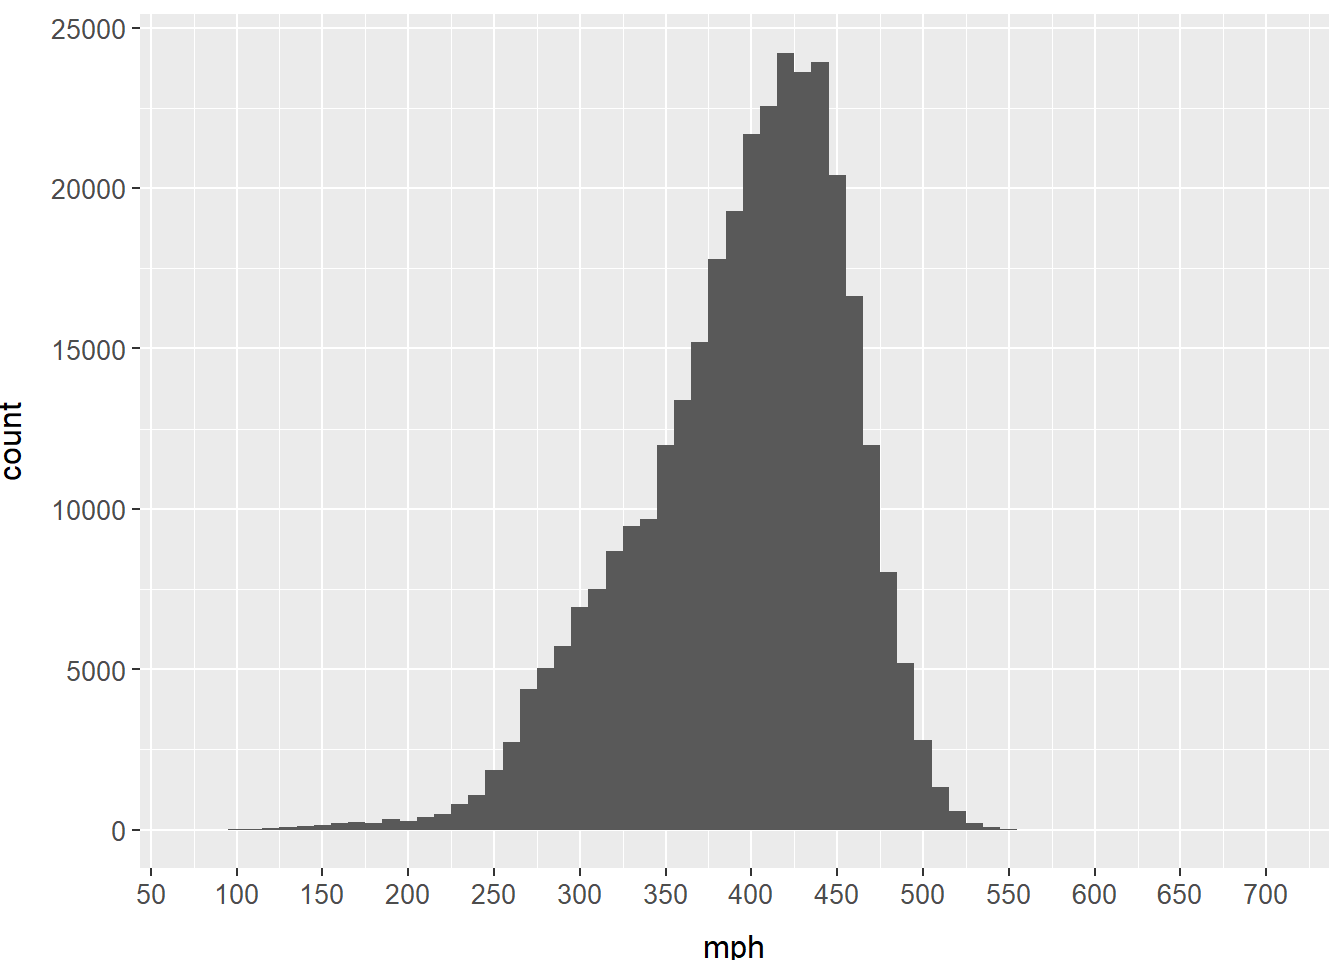
\includegraphics{r4ds_files/figure-latex/unnamed-chunk-79-1.pdf}

\begin{Shaded}
\begin{Highlighting}[]
\NormalTok{standardized }\SpecialCharTok{\%\textgreater{}\%}
    \FunctionTok{mutate}\NormalTok{(}
        \AttributeTok{mph =}\NormalTok{ distance }\SpecialCharTok{/}\NormalTok{ (air\_time }\SpecialCharTok{/} \DecValTok{60}\NormalTok{)}
\NormalTok{    ) }\SpecialCharTok{\%\textgreater{}\%}
    \FunctionTok{arrange}\NormalTok{(}\FunctionTok{desc}\NormalTok{(mph)) }\SpecialCharTok{\%\textgreater{}\%}
    \FunctionTok{select}\NormalTok{(carrier, flight, origin, dest, month, day, mph) }\SpecialCharTok{\%\textgreater{}\%}
    \FunctionTok{head}\NormalTok{(}\DecValTok{10}\NormalTok{)}
\end{Highlighting}
\end{Shaded}

\begin{verbatim}
## # A tibble: 10 x 7
##    carrier flight origin dest  month   day   mph
##    <chr>    <int> <chr>  <chr> <int> <int> <dbl>
##  1 DL        1499 LGA    ATL       5    25  703.
##  2 EV        4667 EWR    MSP       7     2  650.
##  3 EV        4292 EWR    GSP       5    13  648 
##  4 EV        3805 EWR    BNA       3    23  641.
##  5 DL        1902 LGA    PBI       1    12  591.
##  6 DL         315 JFK    SJU      11    17  564 
##  7 B6         707 JFK    SJU       2    21  557.
##  8 AA         936 JFK    STT      11    17  556.
##  9 DL         347 JFK    SJU      11    16  554.
## 10 B6        1503 JFK    SJU      11    16  554.
\end{verbatim}

Algum conhecimento prévio nos indica que a a velocidade superior a 550 milhas por hora são suspeitamente altas.

Note que, em ambas as análises, coicidiram quase todos os voos. Poderíamos fazer análises mais acuradas, se tivéssemos mais conhecimento sobre o domínio de negócio, contudo já podemos concluir que aqueles são os voos suspeitos.
\end{solution}

\hypertarget{exr3-8-7}{%
\subsection*{Exercício 3.8.7}\label{exr3-8-7}}
\addcontentsline{toc}{subsection}{Exercício 3.8.7}

Encontre todos os destinos que são feitos por pelo menos duas companhias. Use essa informação para classificar as companhias.

\begin{solution}
\leavevmode

\begin{Shaded}
\begin{Highlighting}[]
\NormalTok{flights }\SpecialCharTok{\%\textgreater{}\%}
    \FunctionTok{filter}\NormalTok{(}\SpecialCharTok{!}\FunctionTok{is.na}\NormalTok{(arr\_delay)) }\SpecialCharTok{\%\textgreater{}\%}                           \CommentTok{\# Remover os elementos que não tem informação de atraso}
    \FunctionTok{group\_by}\NormalTok{(origin, dest) }\SpecialCharTok{\%\textgreater{}\%}                              \CommentTok{\# Agrupar pela origem e destino}
    \FunctionTok{mutate}\NormalTok{(}
        \AttributeTok{carrier\_count =} \FunctionTok{n\_distinct}\NormalTok{(carrier),                }\CommentTok{\# Calcular quantas empresas fazem o trecho}
        \AttributeTok{arr\_delay\_mean =} \FunctionTok{mean}\NormalTok{(arr\_delay),                   }\CommentTok{\# Calcular o atraso médio do trecho}
        \AttributeTok{arr\_delay\_percent =}\NormalTok{ arr\_delay }\SpecialCharTok{/}\NormalTok{ arr\_delay\_mean      }\CommentTok{\# Calcular a proporção do atraso em relação à média do trecho}
\NormalTok{    ) }\SpecialCharTok{\%\textgreater{}\%}
    \FunctionTok{filter}\NormalTok{(carrier\_count }\SpecialCharTok{\textgreater{}} \DecValTok{1}\NormalTok{) }\SpecialCharTok{\%\textgreater{}\%}                           \CommentTok{\# Considerar apenas trechos operados por mais de uma empresa    }
    \FunctionTok{group\_by}\NormalTok{(origin, dest, carrier) }\SpecialCharTok{\%\textgreater{}\%}
    \FunctionTok{summarise}\NormalTok{(}
        \AttributeTok{arr\_delay =} \FunctionTok{mean}\NormalTok{(arr\_delay\_percent)}
\NormalTok{    ) }\SpecialCharTok{\%\textgreater{}\%}
    \FunctionTok{arrange}\NormalTok{(origin, dest, }\FunctionTok{desc}\NormalTok{(arr\_delay)) }\SpecialCharTok{\%\textgreater{}\%}
    \FunctionTok{head}\NormalTok{(}\DecValTok{25}\NormalTok{)}
\end{Highlighting}
\end{Shaded}

\begin{verbatim}
## `summarise()` has grouped output by 'origin', 'dest'. You can override using
## the `.groups` argument.
\end{verbatim}

\begin{verbatim}
## # A tibble: 25 x 4
## # Groups:   origin, dest [11]
##    origin dest  carrier arr_delay
##    <chr>  <chr> <chr>       <dbl>
##  1 EWR    ATL   EV          1.48 
##  2 EWR    ATL   UA          0.793
##  3 EWR    ATL   DL          0.755
##  4 EWR    ATL   9E         -0.472
##  5 EWR    AUS   WN         23.7  
##  6 EWR    AUS   UA         -9.02 
##  7 EWR    BDL   UA          3.20 
##  8 EWR    BDL   EV          0.962
##  9 EWR    BNA   EV          1.39 
## 10 EWR    BNA   WN         -0.168
## # i 15 more rows
\end{verbatim}

\end{solution}

\hypertarget{fluxo-de-trabalho-scripts}{%
\chapter{Fluxo de trabalho: scripts}\label{fluxo-de-trabalho-scripts}}

\hypertarget{executando-cuxf3digos}{%
\section{Executando códigos}\label{executando-cuxf3digos}}

Não temos exercícios neste seção.

\hypertarget{diagnuxf3sticos-rstudio}{%
\section{Diagnósticos Rstudio}\label{diagnuxf3sticos-rstudio}}

\hypertarget{exr4-2-1}{%
\subsection*{Exercício 4.2.1}\label{exr4-2-1}}
\addcontentsline{toc}{subsection}{Exercício 4.2.1}

Vá para a conta RStudio Tips no Twitter, em \emph{\citet{rstudiotips}}, e escolha uma dica que pareça interessante. Pratique o uso dessa dica!

\begin{solution}
x
\end{solution}

\hypertarget{exr4-2-2}{%
\subsection*{Exercício 4.2.2}\label{exr4-2-2}}
\addcontentsline{toc}{subsection}{Exercício 4.2.2}

Quais outros erros comuns o diagnóstico do RStudio reportará? Leia \emph{\url{http://bit.ly/RStudiocodediag}} para descobrir.

\begin{solution}
x
\end{solution}

\hypertarget{anuxe1lise-exploratuxf3ria-de-dados}{%
\chapter{Análise exploratória de dados}\label{anuxe1lise-exploratuxf3ria-de-dados}}

\hypertarget{introduuxe7uxe3o-2}{%
\section{Introdução}\label{introduuxe7uxe3o-2}}

Não temos exercícios nesta seção.

\hypertarget{perguntas}{%
\section{Perguntas}\label{perguntas}}

Não temos exercícios nesta seção.

\hypertarget{variauxe7uxe3o}{%
\section{Variação}\label{variauxe7uxe3o}}

\hypertarget{exr5-3-1}{%
\subsection*{Exercício 5.3.1}\label{exr5-3-1}}
\addcontentsline{toc}{subsection}{Exercício 5.3.1}

Explore a distribuição de cada variável \texttt{x}, \texttt{y} e \texttt{z} em \texttt{diamonds}. O que você aprende? Pense em um diamante e como você pode determinar qual dimensão é o comprimento, a largura e a profundidade.

\begin{solution}
Por se tratar de variáveis continuas, vamos utilizar um gráfico de densidade (ou histograma) para visualizar os dados.

Como x e y possuem distribuição mais parecisa, acredita-se que tratam-se do comprimento e da largura do diamante, sendo z a profundidade (por ter média menor).

\begin{Shaded}
\begin{Highlighting}[]
\NormalTok{plot }\OtherTok{\textless{}{-}}\NormalTok{ diamonds }\SpecialCharTok{\%\textgreater{}\%} 
          \FunctionTok{ggplot}\NormalTok{() }\SpecialCharTok{+} 
            \FunctionTok{coord\_cartesian}\NormalTok{(}
              \AttributeTok{xlim =} \FunctionTok{c}\NormalTok{(}\DecValTok{0}\NormalTok{, }\DecValTok{10}\NormalTok{),}
              \AttributeTok{ylim =} \FunctionTok{c}\NormalTok{(}\DecValTok{0}\NormalTok{, .}\DecValTok{85}\NormalTok{)}
\NormalTok{            ) }\SpecialCharTok{+}
            \FunctionTok{scale\_x\_continuous}\NormalTok{(}\AttributeTok{breaks =} \FunctionTok{seq}\NormalTok{(}\DecValTok{0}\NormalTok{, }\DecValTok{10}\NormalTok{, }\AttributeTok{by =} \DecValTok{1}\NormalTok{)) }\SpecialCharTok{+}
            \FunctionTok{labs}\NormalTok{(}
              \AttributeTok{y =} \StringTok{""}
\NormalTok{            ) }\SpecialCharTok{+}
\NormalTok{            tema}

\NormalTok{x }\OtherTok{\textless{}{-}}\NormalTok{ plot }\SpecialCharTok{+} \FunctionTok{geom\_density}\NormalTok{(}\FunctionTok{aes}\NormalTok{(x))}
\NormalTok{y }\OtherTok{\textless{}{-}}\NormalTok{ plot }\SpecialCharTok{+} \FunctionTok{geom\_density}\NormalTok{(}\FunctionTok{aes}\NormalTok{(y))}
\NormalTok{z }\OtherTok{\textless{}{-}}\NormalTok{ plot }\SpecialCharTok{+} \FunctionTok{geom\_density}\NormalTok{(}\FunctionTok{aes}\NormalTok{(z))}

\FunctionTok{grid.arrange}\NormalTok{(x, y, z, }\AttributeTok{nrow =} \DecValTok{3}\NormalTok{)}
\end{Highlighting}
\end{Shaded}

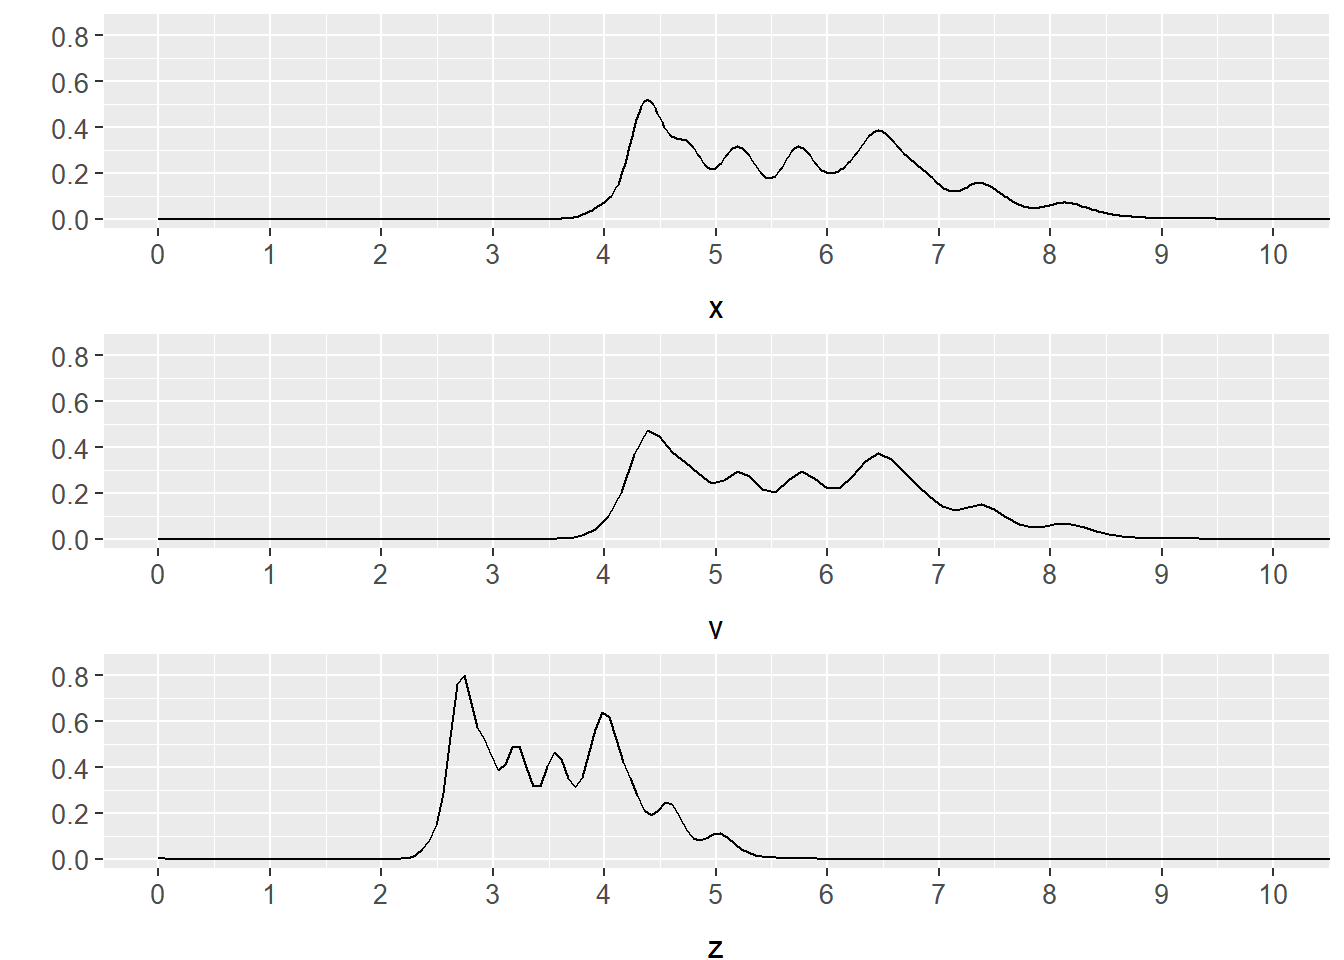
\includegraphics{r4ds_files/figure-latex/unnamed-chunk-81-1.pdf}

\begin{Shaded}
\begin{Highlighting}[]
\NormalTok{diamonds }\SpecialCharTok{\%\textgreater{}\%} 
  \CommentTok{\# Remover os outliers}
  \FunctionTok{filter}\NormalTok{(}\DecValTok{0} \SpecialCharTok{\textless{}}\NormalTok{ x, x }\SpecialCharTok{\textless{}=} \DecValTok{10}\NormalTok{, }\DecValTok{0} \SpecialCharTok{\textless{}}\NormalTok{ y, y }\SpecialCharTok{\textless{}=} \DecValTok{10}\NormalTok{) }\SpecialCharTok{\%\textgreater{}\%}
  \FunctionTok{ggplot}\NormalTok{(}\FunctionTok{aes}\NormalTok{(x, y)) }\SpecialCharTok{+}
    \CommentTok{\# Mostrar a densidade de x e y em conjunto}
    \FunctionTok{geom\_density2d}\NormalTok{() }\SpecialCharTok{+}                      
    \CommentTok{\# Mostrar uma linha guia para visualizar se x e Y crescem de forma }
    \CommentTok{\# proprocional, isto é, se os diamantes são quadrados/redondos}
    \FunctionTok{geom\_abline}\NormalTok{(}
      \FunctionTok{aes}\NormalTok{(}\AttributeTok{intercept =} \DecValTok{0}\NormalTok{, }\AttributeTok{slope =} \DecValTok{1}\NormalTok{),}
      \AttributeTok{linetype =} \StringTok{"dashed"}
\NormalTok{    ) }\SpecialCharTok{+}
    \CommentTok{\# Arrumar a proporção do gráfico}
    \FunctionTok{coord\_cartesian}\NormalTok{(}
      \AttributeTok{xlim =} \FunctionTok{c}\NormalTok{(}\FloatTok{3.5}\NormalTok{, }\FloatTok{8.5}\NormalTok{),}
      \AttributeTok{ylim =} \FunctionTok{c}\NormalTok{(}\FloatTok{3.5}\NormalTok{, }\FloatTok{8.5}\NormalTok{)}
\NormalTok{    ) }\SpecialCharTok{+}
    \CommentTok{\# Aplicar o tema padrão}
\NormalTok{    tema}
\end{Highlighting}
\end{Shaded}

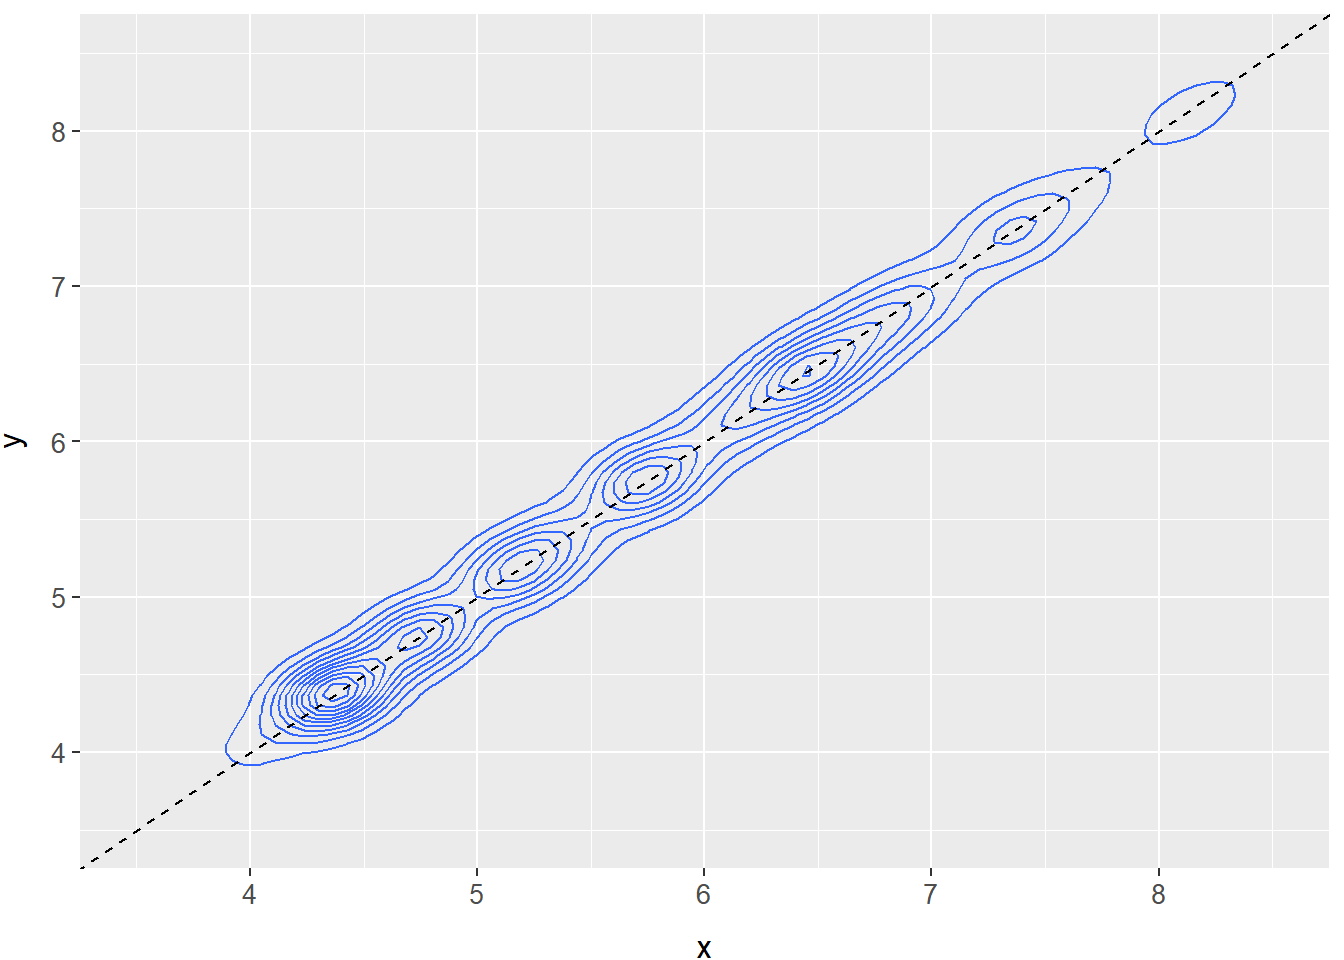
\includegraphics{r4ds_files/figure-latex/unnamed-chunk-82-1.pdf}
\end{solution}

\hypertarget{exr5-3-2}{%
\subsection*{Exercício 5.3.2}\label{exr5-3-2}}
\addcontentsline{toc}{subsection}{Exercício 5.3.2}

Explore a distribuição de \texttt{price}. Você identifica algo incomun ou surpreendente? (Dica: pense cuidadosamente sobre \texttt{binwidth} e certifique-se de experimentar uma ampla gama de valores).

\begin{solution}
\leavevmode

\begin{Shaded}
\begin{Highlighting}[]
\FunctionTok{summary}\NormalTok{(diamonds)}
\end{Highlighting}
\end{Shaded}

\begin{verbatim}
##      carat               cut        color        clarity          depth      
##  Min.   :0.2000   Fair     : 1610   D: 6775   SI1    :13065   Min.   :43.00  
##  1st Qu.:0.4000   Good     : 4906   E: 9797   VS2    :12258   1st Qu.:61.00  
##  Median :0.7000   Very Good:12082   F: 9542   SI2    : 9194   Median :61.80  
##  Mean   :0.7979   Premium  :13791   G:11292   VS1    : 8171   Mean   :61.75  
##  3rd Qu.:1.0400   Ideal    :21551   H: 8304   VVS2   : 5066   3rd Qu.:62.50  
##  Max.   :5.0100                     I: 5422   VVS1   : 3655   Max.   :79.00  
##                                     J: 2808   (Other): 2531                  
##      table           price             x                y         
##  Min.   :43.00   Min.   :  326   Min.   : 0.000   Min.   : 0.000  
##  1st Qu.:56.00   1st Qu.:  950   1st Qu.: 4.710   1st Qu.: 4.720  
##  Median :57.00   Median : 2401   Median : 5.700   Median : 5.710  
##  Mean   :57.46   Mean   : 3933   Mean   : 5.731   Mean   : 5.735  
##  3rd Qu.:59.00   3rd Qu.: 5324   3rd Qu.: 6.540   3rd Qu.: 6.540  
##  Max.   :95.00   Max.   :18823   Max.   :10.740   Max.   :58.900  
##                                                                   
##        z         
##  Min.   : 0.000  
##  1st Qu.: 2.910  
##  Median : 3.530  
##  Mean   : 3.539  
##  3rd Qu.: 4.040  
##  Max.   :31.800  
## 
\end{verbatim}

\begin{Shaded}
\begin{Highlighting}[]
\NormalTok{diamonds }\SpecialCharTok{\%\textgreater{}\%}
    \FunctionTok{ggplot}\NormalTok{(}\FunctionTok{aes}\NormalTok{(}\AttributeTok{x =}\NormalTok{ price)) }\SpecialCharTok{+}
        \FunctionTok{geom\_histogram}\NormalTok{(}\AttributeTok{binwidth =} \DecValTok{100}\NormalTok{) }\SpecialCharTok{+}
\NormalTok{        tema}
\end{Highlighting}
\end{Shaded}

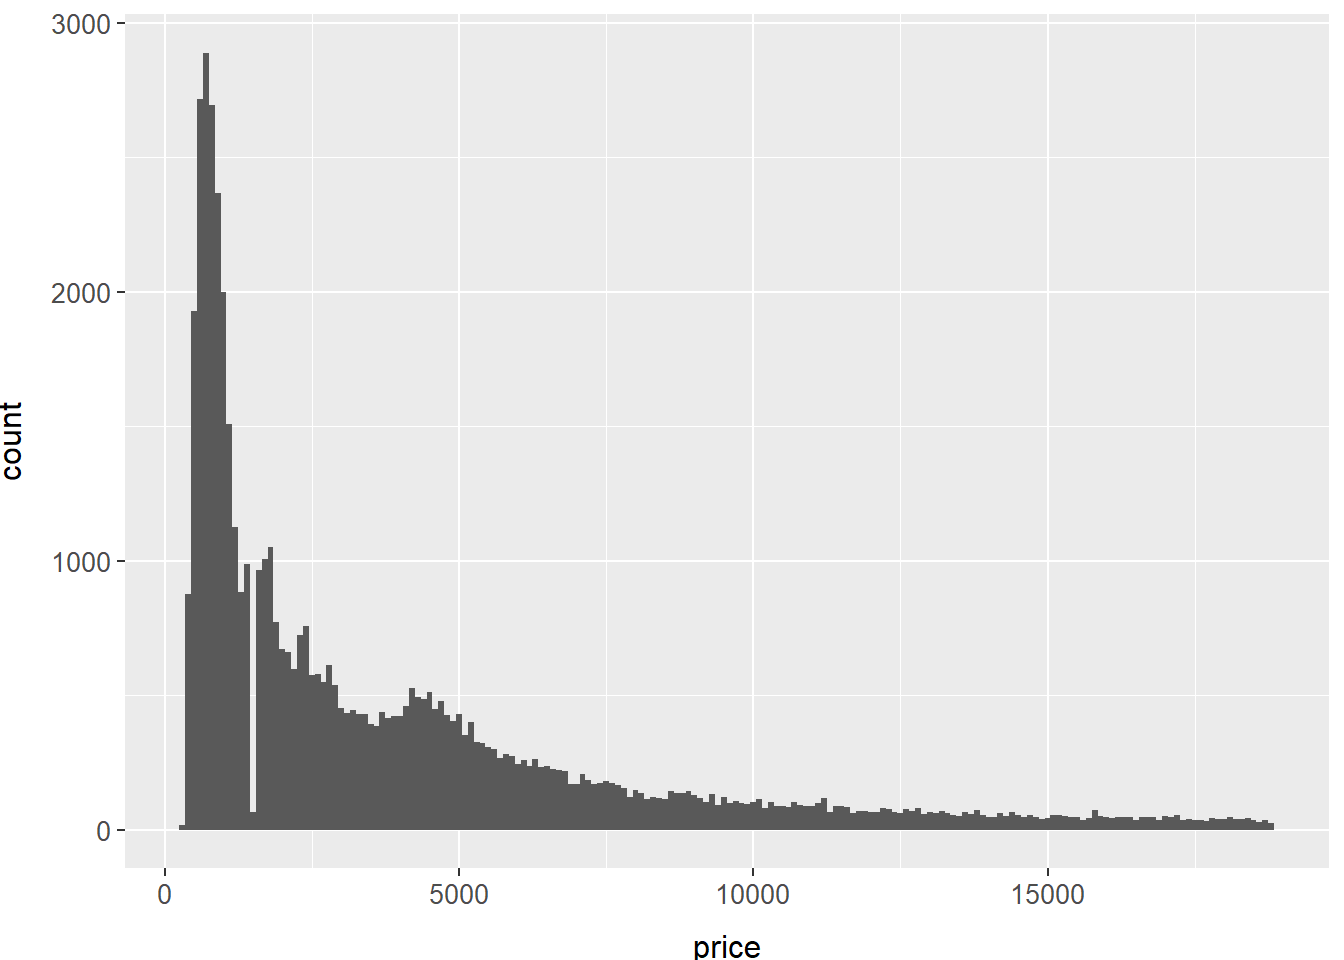
\includegraphics{r4ds_files/figure-latex/unnamed-chunk-84-1.pdf}

\end{solution}

\hypertarget{exr5-3-3}{%
\subsection*{Exercício 5.3.3}\label{exr5-3-3}}
\addcontentsline{toc}{subsection}{Exercício 5.3.3}

Quantos diamantes têm 0,99 quilates? Quantos têm 1 quilate? Qual você acha que é a causa dessa diferença?

\begin{solution}

Existem 23 diamantes com 0.99 quilates, contra 1558 diamantes com 1 quilate. Provavelmente a concentração de diamantes de 1 quilate se deve a arredondamento.

\begin{Shaded}
\begin{Highlighting}[]
\NormalTok{diamonds }\SpecialCharTok{\%\textgreater{}\%}
    \FunctionTok{filter}\NormalTok{(carat }\SpecialCharTok{\textgreater{}=}\NormalTok{ .}\DecValTok{99}\NormalTok{, carat }\SpecialCharTok{\textless{}=} \DecValTok{1}\NormalTok{) }\SpecialCharTok{\%\textgreater{}\%}
    \FunctionTok{count}\NormalTok{(carat)}
\end{Highlighting}
\end{Shaded}

\begin{verbatim}
## # A tibble: 2 x 2
##   carat     n
##   <dbl> <int>
## 1  0.99    23
## 2  1     1558
\end{verbatim}

\end{solution}

\hypertarget{exr5-3-4}{%
\subsection*{Exercício 5.3.4}\label{exr5-3-4}}
\addcontentsline{toc}{subsection}{Exercício 5.3.4}

Compare e contraste \texttt{coord\_cartesian} \emph{versus} \texttt{xlim()} ou \texttt{ylim()} ao dar zoom em um histograma. O que acontece se você não configurar \texttt{binwidth}? O que acontece se você tentar dar zoom para que apenas meia barra seja mostrada?

\begin{solution}
Ao utilizar \texttt{coord\_cartesian()} a restrição nos eixos \texttt{x} e \texttt{y} ocorrem após calculados os valores do gráfico e desenhados os geoms, dessa forma, o cálculo não é afetado pelos limites, apenas é feito o zoom. Já para \texttt{xlim} e \texttt{ylim}, os filtros são aplicados antes da construção do gráfico e as restrições são levadas em consideração, dessa forma, temos pontos que serão realmente descartados, e o leiaute do gráfico acaba ficando bem diferente.

\begin{Shaded}
\begin{Highlighting}[]
\NormalTok{diamonds }\SpecialCharTok{\%\textgreater{}\%}
    \FunctionTok{ggplot}\NormalTok{(}\FunctionTok{aes}\NormalTok{(carat)) }\SpecialCharTok{+}
        \FunctionTok{geom\_histogram}\NormalTok{() }\SpecialCharTok{+}
        \FunctionTok{xlim}\NormalTok{(}\DecValTok{0}\NormalTok{,}\DecValTok{1}\NormalTok{) }\SpecialCharTok{+}
\NormalTok{        tema}
\end{Highlighting}
\end{Shaded}

\begin{verbatim}
## `stat_bin()` using `bins = 30`. Pick better value with `binwidth`.
\end{verbatim}

\begin{verbatim}
## Warning: Removed 17502 rows containing non-finite values (`stat_bin()`).
\end{verbatim}

\begin{verbatim}
## Warning: Removed 2 rows containing missing values (`geom_bar()`).
\end{verbatim}

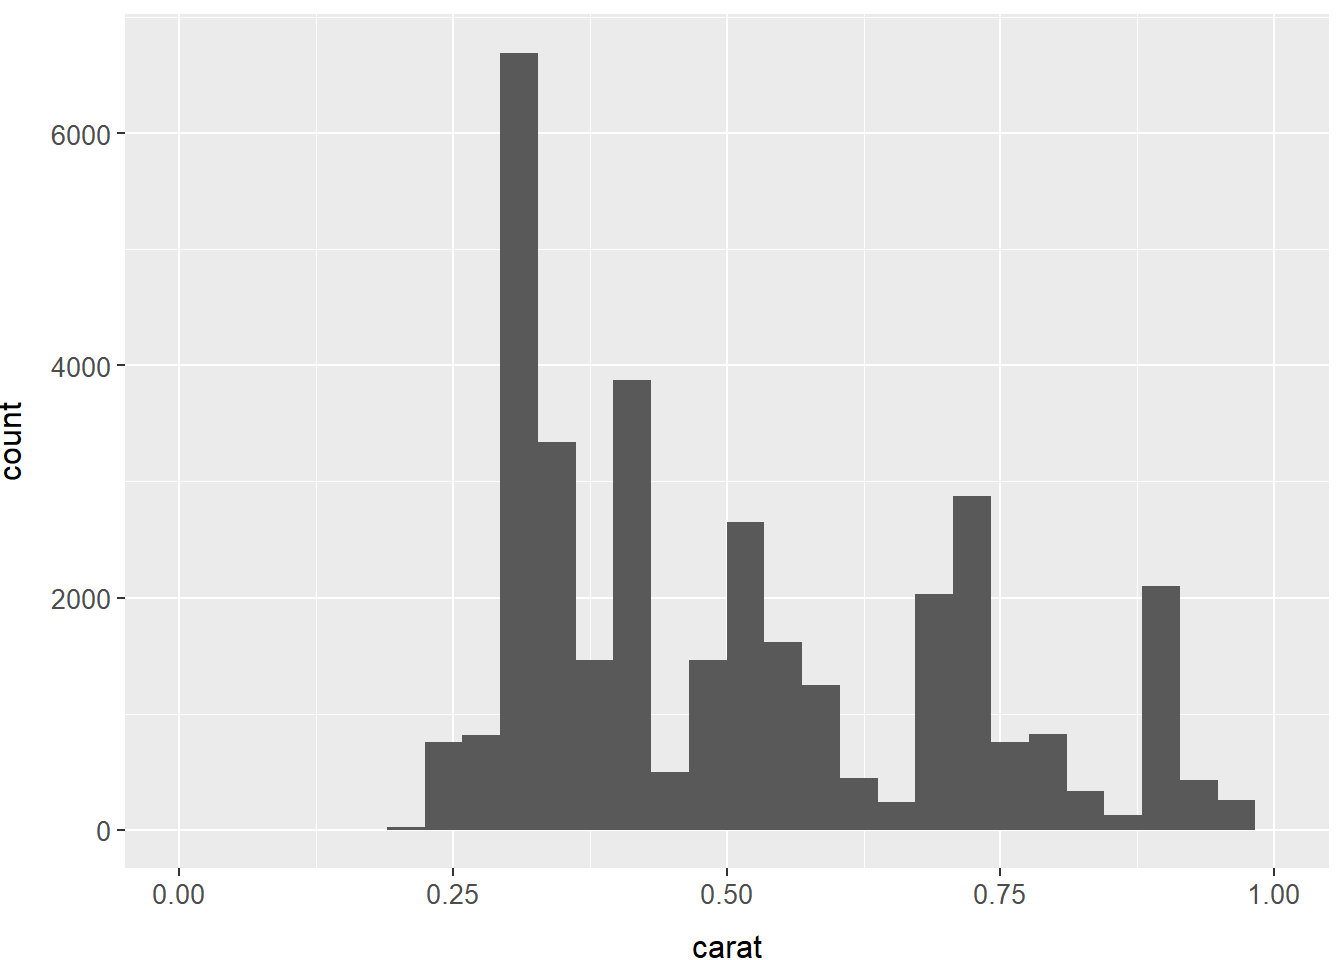
\includegraphics{r4ds_files/figure-latex/unnamed-chunk-86-1.pdf}

\begin{Shaded}
\begin{Highlighting}[]
\NormalTok{diamonds }\SpecialCharTok{\%\textgreater{}\%}
    \FunctionTok{ggplot}\NormalTok{(}\FunctionTok{aes}\NormalTok{(carat)) }\SpecialCharTok{+}
        \FunctionTok{geom\_histogram}\NormalTok{() }\SpecialCharTok{+}
        \FunctionTok{coord\_cartesian}\NormalTok{(}\AttributeTok{xlim =} \FunctionTok{c}\NormalTok{(}\DecValTok{0}\NormalTok{,}\DecValTok{1}\NormalTok{)) }\SpecialCharTok{+}
\NormalTok{        tema}
\end{Highlighting}
\end{Shaded}

\begin{verbatim}
## `stat_bin()` using `bins = 30`. Pick better value with `binwidth`.
\end{verbatim}

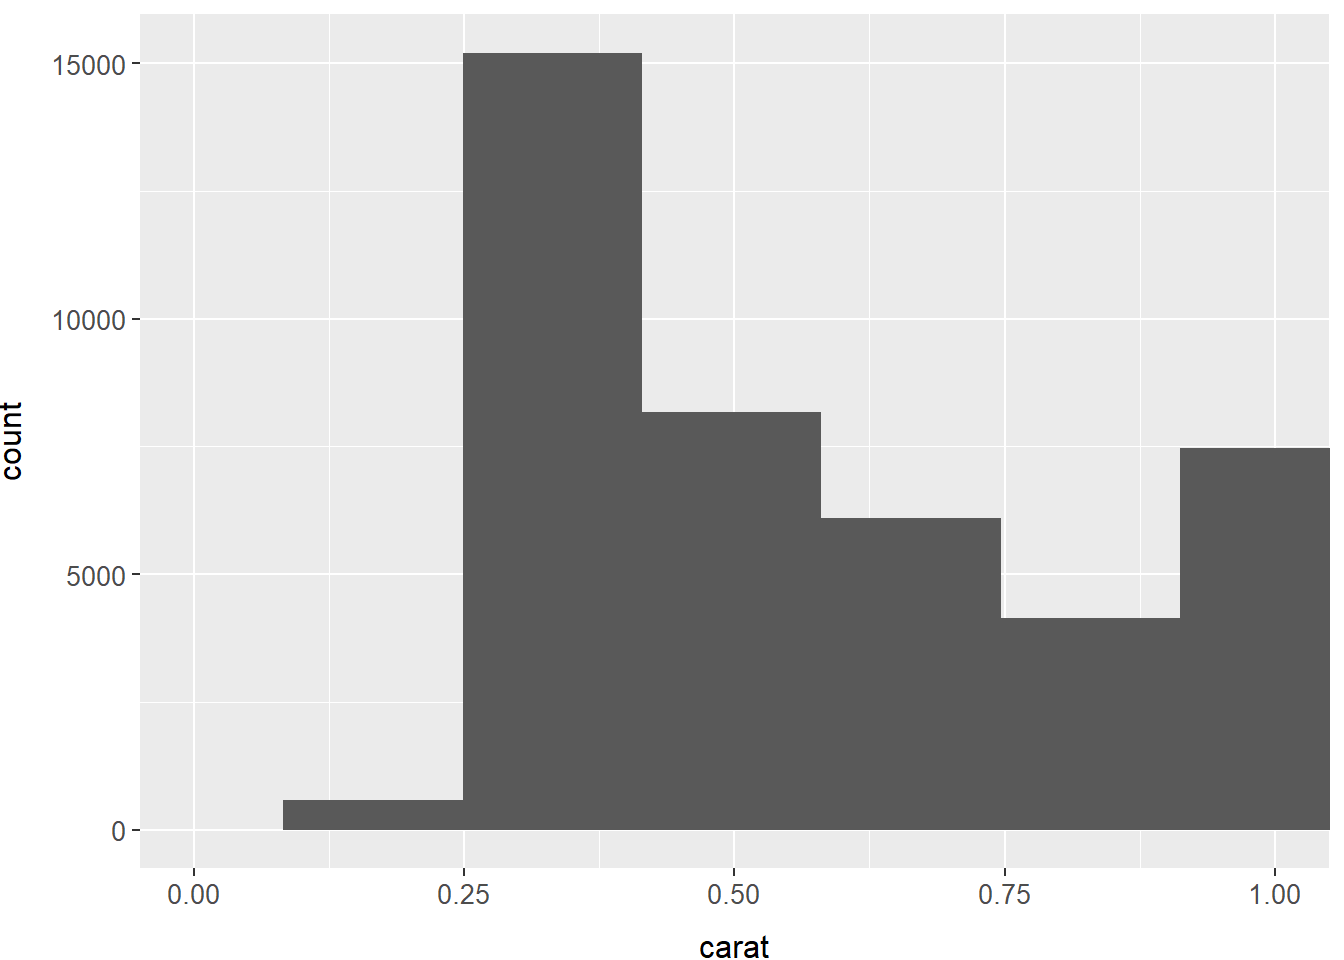
\includegraphics{r4ds_files/figure-latex/unnamed-chunk-87-1.pdf}
\end{solution}

\hypertarget{valores-faltantes}{%
\section{Valores faltantes}\label{valores-faltantes}}

\hypertarget{exr5-4-1}{%
\subsection*{Exercício 5.4.1}\label{exr5-4-1}}
\addcontentsline{toc}{subsection}{Exercício 5.4.1}

O que acontece com valores faltantes em um histograma? O que ocorre com valores faltantes em um gráfico de barras? Por que há uma diferença?

\begin{solution}
A construção de um histograma considera valores continuos, dessa forma os valores faltantes são descartados, uma vez que não é possível dispor valores faltantes na ordenação dos valores (\texttt{NA\ \textgreater{}\ 0} não resulta em um valor lógico). Já para o gráfico de barras, como são considerados valores categóricos, os valores faltantes são exibidos como uma nova categoria.

\begin{Shaded}
\begin{Highlighting}[]
\NormalTok{diamonds2 }\OtherTok{\textless{}{-}}\NormalTok{ diamonds }\SpecialCharTok{\%\textgreater{}\%}
                \FunctionTok{mutate}\NormalTok{(}\AttributeTok{y =} \FunctionTok{ifelse}\NormalTok{(y }\SpecialCharTok{\textless{}} \DecValTok{3} \SpecialCharTok{|}\NormalTok{ y }\SpecialCharTok{\textgreater{}} \DecValTok{20}\NormalTok{, }\ConstantTok{NA}\NormalTok{, y))}

\NormalTok{diamonds2 }\SpecialCharTok{\%\textgreater{}\%}
    \FunctionTok{ggplot}\NormalTok{(}\FunctionTok{aes}\NormalTok{(}\AttributeTok{x =}\NormalTok{ y)) }\SpecialCharTok{+}
        \FunctionTok{geom\_histogram}\NormalTok{() }\SpecialCharTok{+}
\NormalTok{        tema}
\end{Highlighting}
\end{Shaded}

\begin{verbatim}
## `stat_bin()` using `bins = 30`. Pick better value with `binwidth`.
\end{verbatim}

\begin{verbatim}
## Warning: Removed 9 rows containing non-finite values (`stat_bin()`).
\end{verbatim}

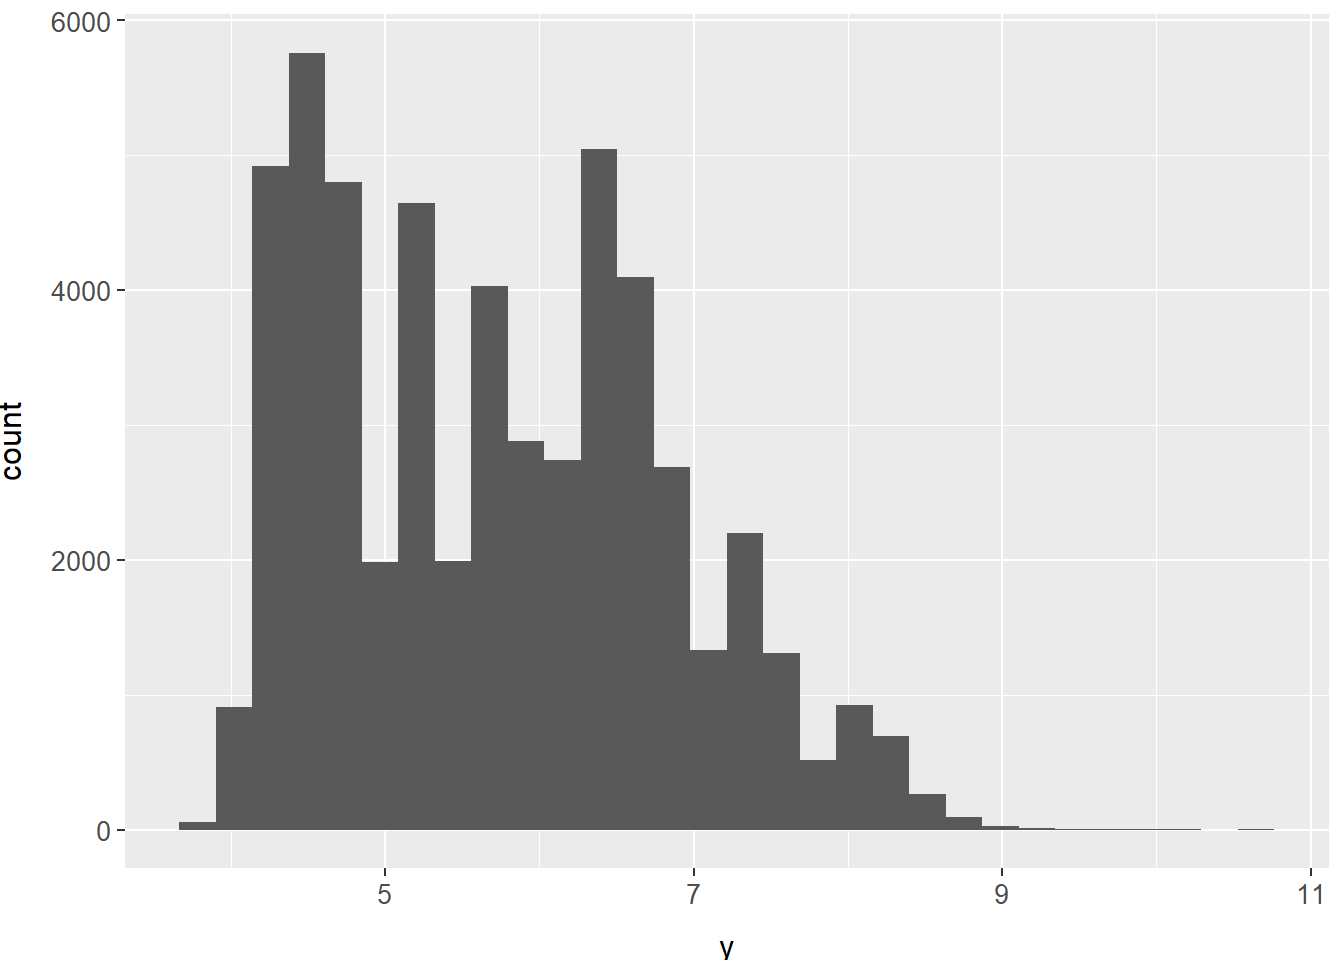
\includegraphics{r4ds_files/figure-latex/unnamed-chunk-88-1.pdf}

\begin{Shaded}
\begin{Highlighting}[]
\NormalTok{diamonds3 }\OtherTok{\textless{}{-}}\NormalTok{ diamonds2 }\SpecialCharTok{\%\textgreater{}\%}
                \FunctionTok{mutate}\NormalTok{(}\AttributeTok{cut =} \FunctionTok{ifelse}\NormalTok{(}\FunctionTok{is.na}\NormalTok{(y), }\ConstantTok{NA}\NormalTok{, }\FunctionTok{as.character}\NormalTok{(cut)))}

\NormalTok{diamonds3 }\SpecialCharTok{\%\textgreater{}\%}    
    \FunctionTok{ggplot}\NormalTok{(}\FunctionTok{aes}\NormalTok{(}\AttributeTok{x =}\NormalTok{ cut)) }\SpecialCharTok{+}
        \FunctionTok{geom\_bar}\NormalTok{() }\SpecialCharTok{+}
\NormalTok{        tema}
\end{Highlighting}
\end{Shaded}

\includegraphics{r4ds_files/figure-latex/unnamed-chunk-89-1.pdf}
\end{solution}

\hypertarget{exr5-4-2}{%
\subsection*{Exercício 5.4.2}\label{exr5-4-2}}
\addcontentsline{toc}{subsection}{Exercício 5.4.2}

O que \texttt{na.rm\ =\ TRUE} faz em \texttt{mean()} e \texttt{sum()}?

\begin{solution}

O parâmetro \texttt{na.rm} serve para indicar que devem ser excluídos da soma ou da média os valores faltantes.

\begin{Shaded}
\begin{Highlighting}[]
\NormalTok{a }\OtherTok{\textless{}{-}} \FunctionTok{c}\NormalTok{(}\DecValTok{1}\NormalTok{, }\DecValTok{2}\NormalTok{, }\DecValTok{3}\NormalTok{, }\DecValTok{4}\NormalTok{, }\ConstantTok{NA}\NormalTok{, }\DecValTok{6}\NormalTok{, }\DecValTok{7}\NormalTok{, }\DecValTok{8}\NormalTok{, }\DecValTok{9}\NormalTok{, }\DecValTok{10}\NormalTok{)}
\FunctionTok{mean}\NormalTok{(a)}
\end{Highlighting}
\end{Shaded}

\begin{verbatim}
## [1] NA
\end{verbatim}

\begin{Shaded}
\begin{Highlighting}[]
\FunctionTok{mean}\NormalTok{(a, }\AttributeTok{na.rm =} \ConstantTok{TRUE}\NormalTok{)}
\end{Highlighting}
\end{Shaded}

\begin{verbatim}
## [1] 5.555556
\end{verbatim}

\begin{Shaded}
\begin{Highlighting}[]
\FunctionTok{sum}\NormalTok{(a)}
\end{Highlighting}
\end{Shaded}

\begin{verbatim}
## [1] NA
\end{verbatim}

\begin{Shaded}
\begin{Highlighting}[]
\FunctionTok{sum}\NormalTok{(a, }\AttributeTok{na.rm =} \ConstantTok{TRUE}\NormalTok{)}
\end{Highlighting}
\end{Shaded}

\begin{verbatim}
## [1] 50
\end{verbatim}

\end{solution}

\hypertarget{covariauxe7uxe3o}{%
\section{Covariação}\label{covariauxe7uxe3o}}

\hypertarget{exr5-5-1}{%
\subsection*{Exercício 5.5.1}\label{exr5-5-1}}
\addcontentsline{toc}{subsection}{Exercício 5.5.1}

Use o que você aprendeu para melhorar a visualização dos tempos de decolagem dos coos cancelados \emph{versus} não cancelados.

\begin{solution}
\leavevmode

\begin{Shaded}
\begin{Highlighting}[]
\NormalTok{flights }\SpecialCharTok{\%\textgreater{}\%}
    \FunctionTok{mutate}\NormalTok{(}
        \AttributeTok{cancelled =} \FunctionTok{ifelse}\NormalTok{(}\FunctionTok{is.na}\NormalTok{(dep\_time), }\StringTok{"Cancelled"}\NormalTok{, }\StringTok{"Not cancelled"}\NormalTok{),}
        \AttributeTok{sched\_hour =}\NormalTok{ sched\_dep\_time }\SpecialCharTok{\%/\%} \DecValTok{100}\NormalTok{,}
        \AttributeTok{sched\_min =}\NormalTok{ sched\_dep\_time }\SpecialCharTok{\%\%} \DecValTok{100}\NormalTok{,}
        \AttributeTok{sched\_dep\_time =}\NormalTok{ sched\_hour }\SpecialCharTok{+}\NormalTok{ (sched\_min }\SpecialCharTok{/} \DecValTok{60}\NormalTok{)}
\NormalTok{    ) }\SpecialCharTok{\%\textgreater{}\%}    
    \FunctionTok{ggplot}\NormalTok{(}\FunctionTok{aes}\NormalTok{(cancelled, sched\_dep\_time)) }\SpecialCharTok{+}
        \FunctionTok{geom\_boxplot}\NormalTok{() }\SpecialCharTok{+}
\NormalTok{        tema}
\end{Highlighting}
\end{Shaded}

\includegraphics{r4ds_files/figure-latex/unnamed-chunk-91-1.pdf}

\end{solution}

\hypertarget{exr5-5-2}{%
\subsection*{Exercício 5.5.2}\label{exr5-5-2}}
\addcontentsline{toc}{subsection}{Exercício 5.5.2}

Qual variável no conjunto de dados dos diamantes é mais importante para prever o preço de um diamante? Como essa variável está correlacionada ao corte (\texttt{cut})? Por que a combinação desses dois relacionamentos leva a diamantes de menor qualidade serem mais caros?

\begin{solution}
Vamos considerar na análise as seguintes variáveis: \texttt{carat}, \texttt{cut}, \texttt{color} e \texttt{clarity}.

Para ãvaliar a correlação entre \texttt{carat} e \texttt{price} (duas variáveis contínuas), podemos usar \texttt{geom\_point()}, \texttt{geom\_boxplot()} com a variável independente discretizada ou \texttt{geom\_quantile()}. Vamos avaliar o melhor dos cenários:

\begin{Shaded}
\begin{Highlighting}[]
\NormalTok{diamonds }\SpecialCharTok{\%\textgreater{}\%} 
    \FunctionTok{ggplot}\NormalTok{(}\FunctionTok{aes}\NormalTok{(carat, price)) }\SpecialCharTok{+}
        \FunctionTok{geom\_point}\NormalTok{() }\SpecialCharTok{+}
\NormalTok{        tema}
\end{Highlighting}
\end{Shaded}

\includegraphics{r4ds_files/figure-latex/unnamed-chunk-92-1.pdf}

\begin{Shaded}
\begin{Highlighting}[]
\NormalTok{diamonds }\SpecialCharTok{\%\textgreater{}\%}
    \FunctionTok{ggplot}\NormalTok{(}\FunctionTok{aes}\NormalTok{(carat, price)) }\SpecialCharTok{+}
        \FunctionTok{geom\_boxplot}\NormalTok{(}\FunctionTok{aes}\NormalTok{(}\AttributeTok{group =} \FunctionTok{cut\_width}\NormalTok{(carat, .}\DecValTok{1}\NormalTok{))) }\SpecialCharTok{+}
\NormalTok{        tema}
\end{Highlighting}
\end{Shaded}

\includegraphics{r4ds_files/figure-latex/unnamed-chunk-93-1.pdf}

Com base nas imagens acima, podemos ver que existe uma relação positiva entre \texttt{carat} e \texttt{price}, o que indica que possivelmente essas duas variáveis estão bem correlacionadas. Note ainda que a representação via boxplot ficou um pouco melhor do que a representação por pontos.

Vamos agora avaliar a variável \texttt{cut}. Por se tratar de uma variável discreta, podemos utilizar \texttt{geom\_col()}, \texttt{geom\_boxplot()}, \texttt{geom\_dotplot()} ou \texttt{geom\_violin()}. Vamos avaliar cada um deles.

\begin{Shaded}
\begin{Highlighting}[]
\NormalTok{diamonds }\SpecialCharTok{\%\textgreater{}\%}
    \FunctionTok{ggplot}\NormalTok{(}\FunctionTok{aes}\NormalTok{(cut, price)) }\SpecialCharTok{+}
        \FunctionTok{geom\_col}\NormalTok{() }\SpecialCharTok{+}
\NormalTok{        tema}
\end{Highlighting}
\end{Shaded}

\includegraphics{r4ds_files/figure-latex/unnamed-chunk-94-1.pdf}

\begin{Shaded}
\begin{Highlighting}[]
\NormalTok{diamonds }\SpecialCharTok{\%\textgreater{}\%}
    \FunctionTok{ggplot}\NormalTok{(}\FunctionTok{aes}\NormalTok{(cut, }\AttributeTok{y =}\NormalTok{ price)) }\SpecialCharTok{+}
        \FunctionTok{geom\_boxplot}\NormalTok{() }\SpecialCharTok{+}
\NormalTok{        tema}
\end{Highlighting}
\end{Shaded}

\includegraphics{r4ds_files/figure-latex/unnamed-chunk-95-1.pdf}

\begin{Shaded}
\begin{Highlighting}[]
\NormalTok{diamonds }\SpecialCharTok{\%\textgreater{}\%}
    \FunctionTok{ggplot}\NormalTok{(}\FunctionTok{aes}\NormalTok{(cut, price)) }\SpecialCharTok{+}
        \FunctionTok{geom\_dotplot}\NormalTok{(}\AttributeTok{binaxis =} \StringTok{"y"}\NormalTok{) }\SpecialCharTok{+}
\NormalTok{        tema}
\end{Highlighting}
\end{Shaded}

\begin{verbatim}
## Bin width defaults to 1/30 of the range of the data. Pick better value with
## `binwidth`.
\end{verbatim}

\includegraphics{r4ds_files/figure-latex/unnamed-chunk-96-1.pdf}

\begin{Shaded}
\begin{Highlighting}[]
\NormalTok{diamonds }\SpecialCharTok{\%\textgreater{}\%}
    \FunctionTok{ggplot}\NormalTok{(}\FunctionTok{aes}\NormalTok{(cut, price)) }\SpecialCharTok{+}
        \FunctionTok{geom\_violin}\NormalTok{(}\AttributeTok{scale =} \StringTok{"area"}\NormalTok{) }\SpecialCharTok{+}
\NormalTok{        tema}
\end{Highlighting}
\end{Shaded}

\includegraphics{r4ds_files/figure-latex/unnamed-chunk-97-1.pdf}

Notamos que os gráficos gerados por \texttt{geom\_col()} e \texttt{geom\_dotplot()} não geraram nenhum resultado interessante. Este devido à poluição visual e aquele devido a mostrar uma contagem dos elementos em cada grupo, e não a associação entre as variáveis.

Tanto com \texttt{geom\_boxplot()}, quanto com \texttt{geom\_violin()}, podemos perceber que há uma correlação negativa muito fraca entre as variáveis e, desta forma, podemos considerar que \texttt{cut} não é interessante para predizer os preços dos diamantes.

Sigamos para a variável \texttt{color}:

\begin{Shaded}
\begin{Highlighting}[]
\NormalTok{diamonds }\SpecialCharTok{\%\textgreater{}\%} 
    \FunctionTok{ggplot}\NormalTok{(}\FunctionTok{aes}\NormalTok{(color, price)) }\SpecialCharTok{+}
        \FunctionTok{geom\_boxplot}\NormalTok{() }\SpecialCharTok{+}
\NormalTok{        tema}
\end{Highlighting}
\end{Shaded}

\includegraphics{r4ds_files/figure-latex/unnamed-chunk-98-1.pdf}

\begin{Shaded}
\begin{Highlighting}[]
\NormalTok{diamonds }\SpecialCharTok{\%\textgreater{}\%} 
    \FunctionTok{ggplot}\NormalTok{(}\FunctionTok{aes}\NormalTok{(color, price)) }\SpecialCharTok{+}
        \FunctionTok{geom\_violin}\NormalTok{(}\AttributeTok{scale =} \StringTok{"area"}\NormalTok{) }\SpecialCharTok{+}
\NormalTok{        tema}
\end{Highlighting}
\end{Shaded}

\includegraphics{r4ds_files/figure-latex/unnamed-chunk-99-1.pdf}

Como podemos perceber, a relação entre as variáveis não é significativa, portanto, descartaremos \texttt{color}.

Seguindo em frente, precisamos avaliar a variável \texttt{clarity}:

\begin{Shaded}
\begin{Highlighting}[]
\NormalTok{diamonds }\SpecialCharTok{\%\textgreater{}\%} 
    \FunctionTok{ggplot}\NormalTok{(}\FunctionTok{aes}\NormalTok{(clarity, price)) }\SpecialCharTok{+}
        \FunctionTok{geom\_boxplot}\NormalTok{() }\SpecialCharTok{+}
\NormalTok{        tema}
\end{Highlighting}
\end{Shaded}

\includegraphics{r4ds_files/figure-latex/unnamed-chunk-100-1.pdf}

\begin{Shaded}
\begin{Highlighting}[]
\NormalTok{diamonds }\SpecialCharTok{\%\textgreater{}\%} 
    \FunctionTok{ggplot}\NormalTok{(}\FunctionTok{aes}\NormalTok{(color, price)) }\SpecialCharTok{+}
        \FunctionTok{geom\_violin}\NormalTok{(}\AttributeTok{scale =} \StringTok{"area"}\NormalTok{) }\SpecialCharTok{+}
\NormalTok{        tema}
\end{Highlighting}
\end{Shaded}

\includegraphics{r4ds_files/figure-latex/unnamed-chunk-101-1.pdf}

Notamos também que a variável não tem correação com o preço.

Concluímos, portanto, que a melhor variável para predizer o preço do diamante é \texttt{carat}.

Agora, avaliaremos a relação entre \texttt{carat} e \texttt{cut}.

\begin{Shaded}
\begin{Highlighting}[]
\NormalTok{diamonds }\SpecialCharTok{\%\textgreater{}\%}
    \FunctionTok{ggplot}\NormalTok{(}\FunctionTok{aes}\NormalTok{(cut, carat)) }\SpecialCharTok{+}
        \FunctionTok{geom\_boxplot}\NormalTok{() }\SpecialCharTok{+}
\NormalTok{        tema}
\end{Highlighting}
\end{Shaded}

\includegraphics{r4ds_files/figure-latex/unnamed-chunk-102-1.pdf}

Há uma relação negativa muito leve entre \texttt{cut} e \texttt{carat}, mas isso não é suficiente para dizer que uma impacta na outra. Há grande variabilidade de \texttt{carat} dentro de cada tipo de corte (\texttt{cut}) e, nota-se, os diamantes de grande quilate (provavelmente pedras grandes), tem um corte apenas justo. Isso pode se dar ao fato de que, quanto menor o diamante, melhor precisa ser o corte para que se consiga um bom valor. Além disso, é presumível que é mais fácil vender um diamante pequeno do que um grande, por isso talvez o preço não seja tão alto.
\end{solution}

\hypertarget{exr5-5-3}{%
\subsection*{Exercício 5.5.3}\label{exr5-5-3}}
\addcontentsline{toc}{subsection}{Exercício 5.5.3}

Instale o pacote \textbf{ggstance} e crie um boxplot horizontal. Como isso se compara a usar \texttt{coord\_flip()}?

\begin{solution}
\leavevmode

\begin{Shaded}
\begin{Highlighting}[]
\FunctionTok{library}\NormalTok{(ggstance)}
\end{Highlighting}
\end{Shaded}

\begin{verbatim}
## 
## Attaching package: 'ggstance'
\end{verbatim}

\begin{verbatim}
## The following objects are masked from 'package:ggplot2':
## 
##     geom_errorbarh, GeomErrorbarh
\end{verbatim}

\begin{Shaded}
\begin{Highlighting}[]
\NormalTok{diamonds }\SpecialCharTok{\%\textgreater{}\%}
    \FunctionTok{ggplot}\NormalTok{(}\FunctionTok{aes}\NormalTok{(carat, cut)) }\SpecialCharTok{+}
        \FunctionTok{geom\_boxploth}\NormalTok{() }\SpecialCharTok{+}
\NormalTok{        tema}
\end{Highlighting}
\end{Shaded}

\begin{verbatim}
## Warning: The following aesthetics were dropped during statistical transformation: x
## i This can happen when ggplot fails to infer the correct grouping structure in
##   the data.
## i Did you forget to specify a `group` aesthetic or to convert a numerical
##   variable into a factor?
\end{verbatim}

\begin{verbatim}
## Warning: Using the `size` aesthetic with geom_segment was deprecated in ggplot2 3.4.0.
## i Please use the `linewidth` aesthetic instead.
## This warning is displayed once every 8 hours.
## Call `lifecycle::last_lifecycle_warnings()` to see where this warning was
## generated.
\end{verbatim}

\begin{verbatim}
## Warning: Using the `size` aesthetic with geom_polygon was deprecated in ggplot2 3.4.0.
## i Please use the `linewidth` aesthetic instead.
## This warning is displayed once every 8 hours.
## Call `lifecycle::last_lifecycle_warnings()` to see where this warning was
## generated.
\end{verbatim}

\includegraphics{r4ds_files/figure-latex/unnamed-chunk-103-1.pdf}

\begin{Shaded}
\begin{Highlighting}[]
\NormalTok{diamonds }\SpecialCharTok{\%\textgreater{}\%}
    \FunctionTok{ggplot}\NormalTok{(}\FunctionTok{aes}\NormalTok{(cut, carat)) }\SpecialCharTok{+}
        \FunctionTok{geom\_boxplot}\NormalTok{() }\SpecialCharTok{+}
        \FunctionTok{coord\_flip}\NormalTok{() }\SpecialCharTok{+}
\NormalTok{        tema}
\end{Highlighting}
\end{Shaded}

\includegraphics{r4ds_files/figure-latex/unnamed-chunk-104-1.pdf}

A diferença está apenas no mapeamento.

\end{solution}

\hypertarget{exr5-5-4}{%
\subsection*{Exercício 5.5.4}\label{exr5-5-4}}
\addcontentsline{toc}{subsection}{Exercício 5.5.4}

Um problema com boxplots é que eles foram desenvolvidos em uma era de conjuntos de dados muito menores e tendem a exibir um número proibitivamente grande de ``valores fora da curva''. Uma abordagem para remediar esse problema é o \emph{letter value plot} . Instale o \textbf{lvplot} e tente usar \texttt{geom\_lv()} para exibir a distribuição de preço \emph{versus} corte. O que você aprendeu? Como você interpreta os gráficos?

\begin{solution}
???

\begin{Shaded}
\begin{Highlighting}[]
\FunctionTok{library}\NormalTok{(lvplot)}

\NormalTok{diamonds }\SpecialCharTok{\%\textgreater{}\%}
    \FunctionTok{ggplot}\NormalTok{(}\FunctionTok{aes}\NormalTok{(cut, price)) }\SpecialCharTok{+}
        \FunctionTok{geom\_lv}\NormalTok{(}\AttributeTok{width.method =} \StringTok{"height"}\NormalTok{) }\SpecialCharTok{+}        
\NormalTok{        tema}
\end{Highlighting}
\end{Shaded}

\includegraphics{r4ds_files/figure-latex/unnamed-chunk-105-1.pdf}
\end{solution}

\hypertarget{exr5-5-5}{%
\subsection*{Exercício 5.5.5}\label{exr5-5-5}}
\addcontentsline{toc}{subsection}{Exercício 5.5.5}

Compare e contraste \texttt{geom\_violin()} com \texttt{geom\_histogram()} facetado, ou um \texttt{geom\_freqpoly()} colorido. Quais são os prós e contras de cada método?

\begin{solution}
Com o polígono de frequência é mais fácil comparar os grupos, uma vez que as linhas são sobrepostas, contudo muitas vezes pode se tornar complicado visualizar o comportamento/variação de cada grupo individualmente. O violino e o histograma permitem visualizar a distribuição em cada grupo, contudo fica mais complicado fazer a comparação.

\begin{Shaded}
\begin{Highlighting}[]
\CommentTok{\# Violin}
\NormalTok{diamonds }\SpecialCharTok{\%\textgreater{}\%}
    \FunctionTok{ggplot}\NormalTok{(}\FunctionTok{aes}\NormalTok{(cut, price)) }\SpecialCharTok{+}
        \FunctionTok{geom\_violin}\NormalTok{() }\SpecialCharTok{+}
        \FunctionTok{coord\_flip}\NormalTok{() }\SpecialCharTok{+}
\NormalTok{        tema}
\end{Highlighting}
\end{Shaded}

\includegraphics{r4ds_files/figure-latex/unnamed-chunk-106-1.pdf}

\begin{Shaded}
\begin{Highlighting}[]
\CommentTok{\# Histogram}
\NormalTok{diamonds }\SpecialCharTok{\%\textgreater{}\%}
    \FunctionTok{ggplot}\NormalTok{(}\FunctionTok{aes}\NormalTok{(price)) }\SpecialCharTok{+}
        \FunctionTok{geom\_histogram}\NormalTok{() }\SpecialCharTok{+}
        \FunctionTok{facet\_wrap}\NormalTok{(}\SpecialCharTok{\textasciitilde{}}\NormalTok{ cut, }\AttributeTok{ncol =} \DecValTok{1}\NormalTok{, }\AttributeTok{scale =} \StringTok{"free\_y"}\NormalTok{) }\SpecialCharTok{+}
\NormalTok{        tema}
\end{Highlighting}
\end{Shaded}

\begin{verbatim}
## `stat_bin()` using `bins = 30`. Pick better value with `binwidth`.
\end{verbatim}

\includegraphics{r4ds_files/figure-latex/unnamed-chunk-106-2.pdf}

\begin{Shaded}
\begin{Highlighting}[]
\CommentTok{\#Frequency Polygon}
\NormalTok{diamonds }\SpecialCharTok{\%\textgreater{}\%}
    \FunctionTok{ggplot}\NormalTok{(}\FunctionTok{aes}\NormalTok{(price, ..density.., }\AttributeTok{color =}\NormalTok{ cut)) }\SpecialCharTok{+}
    \FunctionTok{geom\_freqpoly}\NormalTok{(}\AttributeTok{binwidth =} \DecValTok{500}\NormalTok{) }\SpecialCharTok{+}
\NormalTok{    tema}
\end{Highlighting}
\end{Shaded}

\begin{verbatim}
## Warning: The dot-dot notation (`..density..`) was deprecated in ggplot2 3.4.0.
## i Please use `after_stat(density)` instead.
## This warning is displayed once every 8 hours.
## Call `lifecycle::last_lifecycle_warnings()` to see where this warning was
## generated.
\end{verbatim}

\includegraphics{r4ds_files/figure-latex/unnamed-chunk-106-3.pdf}
\end{solution}

\hypertarget{exr5-5-6}{%
\subsection*{Exercício 5.5.6}\label{exr5-5-6}}
\addcontentsline{toc}{subsection}{Exercício 5.5.6}

Se você tem um conjunto de dados pequeno, às vezes é útil usar \texttt{geom\_jitter()} para ver a relação entre uma variável contínua e uma categórica. O pacote \textbf{ggbeeswarm} fornece alguns métodos similares a \texttt{geom\_jitter()}. Liste-os e descreva brevemente o que cada um faz.

\begin{solution}
O pacote oferece duas geoms. A primeira, \texttt{geom\_quasirandom()} mistura o \emph{jitter} com a a aparencia do gráfico violino. A segunda, \texttt{geom\_beeswarm()} produz gráficos parecidos com violinos, mas com alguma sobreposição.

Em comparação ao \texttt{geom\_jitter()}, o pacote \texttt{ggbeeswarm()} permite uma melhor visualização dos clusteres, caso existam. No nosso exemplo, os clusters seriam as próprias classes, ele evita que os pontos de uma classe se aproximem demais da classe ao lado, gerando uma melhor visualização. Também mantém mais ou menos agrupados as ``alturas'' no eixo y, isto é, o erro é colocado apenas em uma das direções.

\begin{Shaded}
\begin{Highlighting}[]
\FunctionTok{library}\NormalTok{(ggbeeswarm)}

\NormalTok{mpg }\SpecialCharTok{\%\textgreater{}\%}
    \FunctionTok{ggplot}\NormalTok{(}\FunctionTok{aes}\NormalTok{(class, hwy)) }\SpecialCharTok{+}
        \FunctionTok{geom\_point}\NormalTok{() }\SpecialCharTok{+}
\NormalTok{        tema}
\end{Highlighting}
\end{Shaded}

\includegraphics{r4ds_files/figure-latex/unnamed-chunk-107-1.pdf}

\begin{Shaded}
\begin{Highlighting}[]
\NormalTok{mpg }\SpecialCharTok{\%\textgreater{}\%}
    \FunctionTok{ggplot}\NormalTok{(}\FunctionTok{aes}\NormalTok{(class, hwy)) }\SpecialCharTok{+}
        \FunctionTok{geom\_jitter}\NormalTok{() }\SpecialCharTok{+}
\NormalTok{        tema}
\end{Highlighting}
\end{Shaded}

\includegraphics{r4ds_files/figure-latex/unnamed-chunk-107-2.pdf}

\begin{Shaded}
\begin{Highlighting}[]
\NormalTok{mpg }\SpecialCharTok{\%\textgreater{}\%}
    \FunctionTok{ggplot}\NormalTok{(}\FunctionTok{aes}\NormalTok{(class, hwy)) }\SpecialCharTok{+}
        \FunctionTok{geom\_quasirandom}\NormalTok{() }\SpecialCharTok{+}
\NormalTok{        tema}
\end{Highlighting}
\end{Shaded}

\includegraphics{r4ds_files/figure-latex/unnamed-chunk-107-3.pdf}

\begin{Shaded}
\begin{Highlighting}[]
\NormalTok{mpg }\SpecialCharTok{\%\textgreater{}\%}
    \FunctionTok{ggplot}\NormalTok{(}\FunctionTok{aes}\NormalTok{(class, hwy)) }\SpecialCharTok{+}
        \FunctionTok{geom\_beeswarm}\NormalTok{() }\SpecialCharTok{+}
\NormalTok{        tema}
\end{Highlighting}
\end{Shaded}

\includegraphics{r4ds_files/figure-latex/unnamed-chunk-107-4.pdf}
\end{solution}

\hypertarget{exr5-7-7}{%
\subsection*{Exercício 5.5.7}\label{exr5-7-7}}
\addcontentsline{toc}{subsection}{Exercício 5.5.7}

Como você alteraria a escala do conjunto de dados \texttt{diamonds} para mostrar mais claramente a distribuição de corte dentro de cor ou cor dentro de corte?

\begin{solution}
Pode-se melhorar usando a proporção de \texttt{cut} dentro de \texttt{color}, porém a mudança não foi tão significativa.

\begin{Shaded}
\begin{Highlighting}[]
\NormalTok{diamonds }\SpecialCharTok{\%\textgreater{}\%}
    \FunctionTok{count}\NormalTok{(color, cut) }\SpecialCharTok{\%\textgreater{}\%}
    \FunctionTok{ggplot}\NormalTok{(}\FunctionTok{aes}\NormalTok{(color, cut)) }\SpecialCharTok{+}
        \FunctionTok{geom\_tile}\NormalTok{(}\AttributeTok{mapping =} \FunctionTok{aes}\NormalTok{(}\AttributeTok{fill =}\NormalTok{ n)) }\SpecialCharTok{+} 
\NormalTok{        tema}
\end{Highlighting}
\end{Shaded}

\includegraphics{r4ds_files/figure-latex/unnamed-chunk-108-1.pdf}

\begin{Shaded}
\begin{Highlighting}[]
\NormalTok{diamonds }\SpecialCharTok{\%\textgreater{}\%}
    \FunctionTok{count}\NormalTok{(color, cut) }\SpecialCharTok{\%\textgreater{}\%}
    \FunctionTok{group\_by}\NormalTok{(color) }\SpecialCharTok{\%\textgreater{}\%}
    \FunctionTok{mutate}\NormalTok{(}
        \AttributeTok{prop =}\NormalTok{ n }\SpecialCharTok{/} \FunctionTok{sum}\NormalTok{(n)}
\NormalTok{    ) }\SpecialCharTok{\%\textgreater{}\%}
    \FunctionTok{ggplot}\NormalTok{(}\FunctionTok{aes}\NormalTok{(color, cut)) }\SpecialCharTok{+}
        \FunctionTok{geom\_tile}\NormalTok{(}\AttributeTok{mapping =} \FunctionTok{aes}\NormalTok{(}\AttributeTok{fill =}\NormalTok{ prop)) }\SpecialCharTok{+} 
\NormalTok{        tema}
\end{Highlighting}
\end{Shaded}

\includegraphics{r4ds_files/figure-latex/unnamed-chunk-108-2.pdf}
\end{solution}

\hypertarget{exr5-5-8}{%
\subsection*{Exercício 5.5.8}\label{exr5-5-8}}
\addcontentsline{toc}{subsection}{Exercício 5.5.8}

Use \texttt{geom\_tile()} junto de \textbf{dplyr} para explorar como os atrasos médios dos voos variam por destino e mês. O que dificulta a leitura do gráfico? Como você poderia melhorá-lo?

\begin{solution}
???

\begin{Shaded}
\begin{Highlighting}[]
\NormalTok{flights }\SpecialCharTok{\%\textgreater{}\%}
    \FunctionTok{group\_by}\NormalTok{(month, dest) }\SpecialCharTok{\%\textgreater{}\%}                           \CommentTok{\# Agrupar por mês e destino}
    \FunctionTok{summarise}\NormalTok{(}
        \AttributeTok{dep\_delay =} \FunctionTok{mean}\NormalTok{(dep\_delay, }\AttributeTok{na.rm =} \ConstantTok{TRUE}\NormalTok{)       }\CommentTok{\# Calcular o atraso médio}
\NormalTok{    ) }\SpecialCharTok{\%\textgreater{}\%}
    \FunctionTok{group\_by}\NormalTok{(dest) }\SpecialCharTok{\%\textgreater{}\%}                                  \CommentTok{\# Agrupar pelo destino}
    \FunctionTok{filter}\NormalTok{(}\FunctionTok{n}\NormalTok{() }\SpecialCharTok{==} \DecValTok{12}\NormalTok{) }\SpecialCharTok{\%\textgreater{}\%}                               \CommentTok{\# Selecionar apenas aqueles destinos que tem informação de todos os meses}
    \FunctionTok{ungroup}\NormalTok{() }\SpecialCharTok{\%\textgreater{}\%}                                       \CommentTok{\# Desagrupa pelo destino}
    \FunctionTok{ggplot}\NormalTok{(}\FunctionTok{aes}\NormalTok{(}\FunctionTok{factor}\NormalTok{(month), dest, }\AttributeTok{fill =}\NormalTok{ dep\_delay)) }\SpecialCharTok{+}
        \FunctionTok{geom\_tile}\NormalTok{()}
\end{Highlighting}
\end{Shaded}

\begin{verbatim}
## `summarise()` has grouped output by 'month'. You can override using the
## `.groups` argument.
\end{verbatim}

\includegraphics{r4ds_files/figure-latex/unnamed-chunk-109-1.pdf}
\end{solution}

\hypertarget{exr5-5-9}{%
\subsection*{Exercício 5.5.9}\label{exr5-5-9}}
\addcontentsline{toc}{subsection}{Exercício 5.5.9}

Por que é um pouco melhor usar \texttt{aes(x\ =\ color,\ y\ =\ cut)} em vez de \texttt{aes(c\ =\ cut,\ y\ =\ color)} no exemplo anterior?

\begin{solution}
???

\begin{Shaded}
\begin{Highlighting}[]
\NormalTok{diamonds }\SpecialCharTok{\%\textgreater{}\%}
    \FunctionTok{count}\NormalTok{(color, cut) }\SpecialCharTok{\%\textgreater{}\%}    
    \FunctionTok{ggplot}\NormalTok{(}\FunctionTok{aes}\NormalTok{(color, cut)) }\SpecialCharTok{+}
        \FunctionTok{geom\_tile}\NormalTok{(}\AttributeTok{mapping =} \FunctionTok{aes}\NormalTok{(}\AttributeTok{fill =}\NormalTok{ n)) }\SpecialCharTok{+} 
\NormalTok{        tema}
\end{Highlighting}
\end{Shaded}

\includegraphics{r4ds_files/figure-latex/unnamed-chunk-110-1.pdf}

\begin{Shaded}
\begin{Highlighting}[]
\NormalTok{diamonds }\SpecialCharTok{\%\textgreater{}\%}
    \FunctionTok{count}\NormalTok{(cut, color) }\SpecialCharTok{\%\textgreater{}\%}    
    \FunctionTok{ggplot}\NormalTok{(}\FunctionTok{aes}\NormalTok{(cut, color)) }\SpecialCharTok{+}
        \FunctionTok{geom\_tile}\NormalTok{(}\AttributeTok{mapping =} \FunctionTok{aes}\NormalTok{(}\AttributeTok{fill =}\NormalTok{ n)) }\SpecialCharTok{+} 
\NormalTok{        tema}
\end{Highlighting}
\end{Shaded}

\includegraphics{r4ds_files/figure-latex/unnamed-chunk-110-2.pdf}
\end{solution}

\hypertarget{exr5-5-10}{%
\subsection*{Exercício 5.5.10}\label{exr5-5-10}}
\addcontentsline{toc}{subsection}{Exercício 5.5.10}

Em vez de resumir a distribuição condicional com um boxplot, pode-se usar um polígono de frequência. O que você precisa considerar ao usar \texttt{cut\_width()} \emph{versus} \texttt{cut\_number()}? Como isso impacta uma visualização da distribuição 2D de \texttt{carat} e \texttt{price}?

\begin{solution}
Utilizamos \texttt{cut\_width()} quando queremos determinar o tamanho das classes que serão exibidas e \texttt{cut\_number()} quando queremos determinar o número de classes.

Se o número total de classes for muito grande, a visualização fica comprometida. Se for pequeno demais, não captaremos comportamentos importantes.

\begin{Shaded}
\begin{Highlighting}[]
\NormalTok{diamonds }\SpecialCharTok{\%\textgreater{}\%}
    \FunctionTok{ggplot}\NormalTok{(}\FunctionTok{aes}\NormalTok{(carat, price)) }\SpecialCharTok{+}
        \FunctionTok{geom\_boxplot}\NormalTok{(}\FunctionTok{aes}\NormalTok{(}\AttributeTok{group =} \FunctionTok{cut\_number}\NormalTok{(carat, }\DecValTok{5}\NormalTok{)))}
\end{Highlighting}
\end{Shaded}

\includegraphics{r4ds_files/figure-latex/unnamed-chunk-111-1.pdf}

\begin{Shaded}
\begin{Highlighting}[]
\NormalTok{diamonds }\SpecialCharTok{\%\textgreater{}\%}
    \FunctionTok{ggplot}\NormalTok{(}\FunctionTok{aes}\NormalTok{(price)) }\SpecialCharTok{+}
        \FunctionTok{geom\_freqpoly}\NormalTok{(}\FunctionTok{aes}\NormalTok{(}\AttributeTok{color =} \FunctionTok{cut\_number}\NormalTok{(carat, }\DecValTok{5}\NormalTok{))) }\SpecialCharTok{+}
\NormalTok{        tema}
\end{Highlighting}
\end{Shaded}

\begin{verbatim}
## `stat_bin()` using `bins = 30`. Pick better value with `binwidth`.
\end{verbatim}

\includegraphics{r4ds_files/figure-latex/unnamed-chunk-111-2.pdf}

\begin{Shaded}
\begin{Highlighting}[]
\NormalTok{diamonds }\SpecialCharTok{\%\textgreater{}\%}
    \FunctionTok{ggplot}\NormalTok{(}\FunctionTok{aes}\NormalTok{(price)) }\SpecialCharTok{+}
        \FunctionTok{geom\_freqpoly}\NormalTok{(}\FunctionTok{aes}\NormalTok{(}\AttributeTok{color =} \FunctionTok{cut\_width}\NormalTok{(carat, }\DecValTok{1}\NormalTok{))) }\SpecialCharTok{+}
\NormalTok{        tema}
\end{Highlighting}
\end{Shaded}

\begin{verbatim}
## `stat_bin()` using `bins = 30`. Pick better value with `binwidth`.
\end{verbatim}

\includegraphics{r4ds_files/figure-latex/unnamed-chunk-111-3.pdf}
\end{solution}

\hypertarget{exr5-5-11}{%
\subsection*{Exercício 5.5.11}\label{exr5-5-11}}
\addcontentsline{toc}{subsection}{Exercício 5.5.11}

Visualize a distribuição de \texttt{carat}, particionada por \texttt{price}.

\begin{solution}
Inicialmente vamos utilizar boxplot para visualizar a distribuição. Vamos dividir os preços em 10 grupos.

\begin{Shaded}
\begin{Highlighting}[]
\NormalTok{diamonds }\SpecialCharTok{\%\textgreater{}\%}
    \FunctionTok{ggplot}\NormalTok{(}\FunctionTok{aes}\NormalTok{(}\FunctionTok{cut\_number}\NormalTok{(price, }\DecValTok{10}\NormalTok{), carat)) }\SpecialCharTok{+}
        \FunctionTok{geom\_boxplot}\NormalTok{() }\SpecialCharTok{+}
        \FunctionTok{coord\_flip}\NormalTok{() }\SpecialCharTok{+}
\NormalTok{        tema}
\end{Highlighting}
\end{Shaded}

\includegraphics{r4ds_files/figure-latex/unnamed-chunk-112-1.pdf}

Note que, \texttt{cut\_number()} dividiu os grupos de modo a ter a mesma quantidade de registros em cada classe e isso acaba gerando classes de larguras diferentes. É mais fácil comparar classes de mesma largura, por isso vamos refazer a visualização utilizando \texttt{cut\_width()}:

\begin{Shaded}
\begin{Highlighting}[]
\NormalTok{diamonds }\SpecialCharTok{\%\textgreater{}\%}
    \FunctionTok{ggplot}\NormalTok{(}\FunctionTok{aes}\NormalTok{(}\FunctionTok{cut\_width}\NormalTok{(price, }\DecValTok{2000}\NormalTok{), carat)) }\SpecialCharTok{+}
        \FunctionTok{geom\_boxplot}\NormalTok{() }\SpecialCharTok{+}
        \FunctionTok{coord\_flip}\NormalTok{() }\SpecialCharTok{+}
\NormalTok{        tema}
\end{Highlighting}
\end{Shaded}

\includegraphics{r4ds_files/figure-latex/unnamed-chunk-113-1.pdf}

A visualização ficou um pouco melhor, porém temos uma classe que inclui valores negativos. Vamos corrigir isso utilizando o argumento \texttt{boundary}:

\begin{Shaded}
\begin{Highlighting}[]
\NormalTok{diamonds }\SpecialCharTok{\%\textgreater{}\%}
    \FunctionTok{ggplot}\NormalTok{(}\FunctionTok{aes}\NormalTok{(}\FunctionTok{cut\_width}\NormalTok{(price, }\DecValTok{2000}\NormalTok{, }\AttributeTok{boundary =} \DecValTok{0}\NormalTok{), carat)) }\SpecialCharTok{+}
        \FunctionTok{geom\_boxplot}\NormalTok{() }\SpecialCharTok{+}
        \FunctionTok{coord\_flip}\NormalTok{() }\SpecialCharTok{+}
\NormalTok{        tema}
\end{Highlighting}
\end{Shaded}

\includegraphics{r4ds_files/figure-latex/unnamed-chunk-114-1.pdf}

Como existem muitos \emph{outliers}, vamos tentar utilizar o \emph{letter value}:

\begin{Shaded}
\begin{Highlighting}[]
\NormalTok{diamonds }\SpecialCharTok{\%\textgreater{}\%}
    \FunctionTok{ggplot}\NormalTok{(}\FunctionTok{aes}\NormalTok{(}\FunctionTok{cut\_width}\NormalTok{(price, }\DecValTok{2000}\NormalTok{, }\AttributeTok{boundary =} \DecValTok{0}\NormalTok{), carat)) }\SpecialCharTok{+}
        \FunctionTok{geom\_lv}\NormalTok{() }\SpecialCharTok{+}
        \FunctionTok{coord\_flip}\NormalTok{() }\SpecialCharTok{+}
\NormalTok{        tema}
\end{Highlighting}
\end{Shaded}

\includegraphics{r4ds_files/figure-latex/unnamed-chunk-115-1.pdf}

Para melhorar a visualização das classes, vamos também mudar a unidade de \texttt{price} de dolares para milhares de dólares, basta dividirmos os valores por 1000:

\begin{Shaded}
\begin{Highlighting}[]
\NormalTok{diamonds }\SpecialCharTok{\%\textgreater{}\%}
    \FunctionTok{mutate}\NormalTok{ (}\AttributeTok{price =}\NormalTok{ price }\SpecialCharTok{/} \DecValTok{1000}\NormalTok{) }\SpecialCharTok{\%\textgreater{}\%}
    \FunctionTok{ggplot}\NormalTok{(}\FunctionTok{aes}\NormalTok{(}\FunctionTok{cut\_width}\NormalTok{(price, }\DecValTok{2}\NormalTok{, }\AttributeTok{boundary =} \DecValTok{0}\NormalTok{), carat)) }\SpecialCharTok{+}
        \FunctionTok{geom\_lv}\NormalTok{() }\SpecialCharTok{+}
        \FunctionTok{coord\_flip}\NormalTok{() }\SpecialCharTok{+}
\NormalTok{        tema}
\end{Highlighting}
\end{Shaded}

\includegraphics{r4ds_files/figure-latex/unnamed-chunk-116-1.pdf}

Agora vamos melhorar os títulos do gráfico:

\begin{Shaded}
\begin{Highlighting}[]
\NormalTok{diamonds }\SpecialCharTok{\%\textgreater{}\%}
    \FunctionTok{mutate}\NormalTok{ (}\AttributeTok{price =}\NormalTok{ price }\SpecialCharTok{/} \DecValTok{1000}\NormalTok{) }\SpecialCharTok{\%\textgreater{}\%}
    \FunctionTok{ggplot}\NormalTok{(}\FunctionTok{aes}\NormalTok{(}\FunctionTok{cut\_width}\NormalTok{(price, }\DecValTok{2}\NormalTok{, }\AttributeTok{boundary =} \DecValTok{0}\NormalTok{), carat)) }\SpecialCharTok{+}
        \FunctionTok{geom\_lv}\NormalTok{() }\SpecialCharTok{+}
        \FunctionTok{coord\_flip}\NormalTok{() }\SpecialCharTok{+}
        \FunctionTok{labs}\NormalTok{(}
            \AttributeTok{title =} \StringTok{"Distribuição do quilate das pedras por faixa de preço"}\NormalTok{,}
            \AttributeTok{y =} \StringTok{"Quilates"}\NormalTok{,}
            \AttributeTok{x =} \StringTok{"Preço (mil dólares)"}
\NormalTok{        ) }\SpecialCharTok{+}
\NormalTok{        tema}
\end{Highlighting}
\end{Shaded}

\includegraphics{r4ds_files/figure-latex/unnamed-chunk-117-1.pdf}

O gráfico está pronto.

Note que poderíamos ter utilizado a \texttt{geom\_violin()}, porém, neste caso, não teríamos uma visão muito boa dos outliers.

\begin{Shaded}
\begin{Highlighting}[]
\NormalTok{diamonds }\SpecialCharTok{\%\textgreater{}\%}
    \FunctionTok{mutate}\NormalTok{ (}\AttributeTok{price =}\NormalTok{ price }\SpecialCharTok{/} \DecValTok{1000}\NormalTok{) }\SpecialCharTok{\%\textgreater{}\%}
    \FunctionTok{ggplot}\NormalTok{(}\FunctionTok{aes}\NormalTok{(}\FunctionTok{cut\_width}\NormalTok{(price, }\DecValTok{2}\NormalTok{, }\AttributeTok{boundary =} \DecValTok{0}\NormalTok{), carat)) }\SpecialCharTok{+}
        \FunctionTok{geom\_violin}\NormalTok{() }\SpecialCharTok{+}
        \FunctionTok{coord\_flip}\NormalTok{() }\SpecialCharTok{+}
        \FunctionTok{labs}\NormalTok{(}
            \AttributeTok{title =} \StringTok{"Distribuição do quilate das pedras por faixa de preço"}\NormalTok{,}
            \AttributeTok{y =} \StringTok{"Quilates"}\NormalTok{,}
            \AttributeTok{x =} \StringTok{"Preço (mil dólares)"}
\NormalTok{        ) }\SpecialCharTok{+}
\NormalTok{        tema}
\end{Highlighting}
\end{Shaded}

\includegraphics{r4ds_files/figure-latex/unnamed-chunk-118-1.pdf}
\end{solution}

\hypertarget{exr5-5-12}{%
\subsection*{Exercício 5.5.12}\label{exr5-5-12}}
\addcontentsline{toc}{subsection}{Exercício 5.5.12}

Como a distribuição de preços de diamantes muito grandes se compara à de diamantes pequenos? É como você esperava ou isso lhe surpreende?

\begin{solution}
???

\begin{Shaded}
\begin{Highlighting}[]
\NormalTok{diamonds }\SpecialCharTok{\%\textgreater{}\%}
    \FunctionTok{ggplot}\NormalTok{(}\FunctionTok{aes}\NormalTok{(}\FunctionTok{cut\_width}\NormalTok{(carat, }\DecValTok{2}\NormalTok{, }\AttributeTok{boundary =} \DecValTok{0}\NormalTok{), price)) }\SpecialCharTok{+}
        \FunctionTok{geom\_boxplot}\NormalTok{() }\SpecialCharTok{+}
\NormalTok{        tema}
\end{Highlighting}
\end{Shaded}

\includegraphics{r4ds_files/figure-latex/unnamed-chunk-119-1.pdf}
\end{solution}

\hypertarget{exr5-5-13}{%
\subsection*{Exercício 5.5.13}\label{exr5-5-13}}
\addcontentsline{toc}{subsection}{Exercício 5.5.13}

Combine duas técnicas que você aprendeu para visualizar a distribuição combinada de \texttt{cut}, \texttt{carat} e \texttt{price}.

\begin{solution}
\leavevmode

\begin{Shaded}
\begin{Highlighting}[]
\NormalTok{diamonds }\SpecialCharTok{\%\textgreater{}\%}
    \FunctionTok{ggplot}\NormalTok{(}\FunctionTok{aes}\NormalTok{(}\FunctionTok{cut\_number}\NormalTok{(carat, }\DecValTok{5}\NormalTok{), price, }\AttributeTok{color =}\NormalTok{ cut)) }\SpecialCharTok{+}
        \FunctionTok{geom\_boxplot}\NormalTok{() }\SpecialCharTok{+}
\NormalTok{        tema}
\end{Highlighting}
\end{Shaded}

\includegraphics{r4ds_files/figure-latex/unnamed-chunk-120-1.pdf}

\begin{Shaded}
\begin{Highlighting}[]
\NormalTok{diamonds }\SpecialCharTok{\%\textgreater{}\%}
    \FunctionTok{ggplot}\NormalTok{(}\FunctionTok{aes}\NormalTok{(carat, price)) }\SpecialCharTok{+}
        \FunctionTok{geom\_hex}\NormalTok{() }\SpecialCharTok{+}
        \FunctionTok{facet\_wrap}\NormalTok{(}\SpecialCharTok{\textasciitilde{}}\NormalTok{ cut, }\AttributeTok{ncol =} \DecValTok{1}\NormalTok{) }\SpecialCharTok{+}
\NormalTok{        tema}
\end{Highlighting}
\end{Shaded}

\includegraphics{r4ds_files/figure-latex/unnamed-chunk-121-1.pdf}

\begin{Shaded}
\begin{Highlighting}[]
\NormalTok{diamonds }\SpecialCharTok{\%\textgreater{}\%}
    \FunctionTok{ggplot}\NormalTok{(}\FunctionTok{aes}\NormalTok{(}\FunctionTok{cut\_number}\NormalTok{(carat, }\DecValTok{10}\NormalTok{), cut, }\AttributeTok{fill =} \FunctionTok{desc}\NormalTok{(price))) }\SpecialCharTok{+}
        \FunctionTok{geom\_tile}\NormalTok{() }\SpecialCharTok{+}        
\NormalTok{        tema}
\end{Highlighting}
\end{Shaded}

\includegraphics{r4ds_files/figure-latex/unnamed-chunk-122-1.pdf}

\end{solution}

\hypertarget{exr5-5-14}{%
\subsection*{Exercício 5.5.14}\label{exr5-5-14}}
\addcontentsline{toc}{subsection}{Exercício 5.5.14}

Gráficos bidimensionais revelam pontos fora da curva que não são visíveis em gráficos unidimensionais. Por exemplo, alguns pontos no gráfico a seguir tem uma combinação incomum de valores de \texttt{x} e \texttt{y}, que faz pontos ficarem fora da curva, mesmo embora seus valores \texttt{x} e \texttt{y} pareçam normais quando examidanos separadamente.

\begin{Shaded}
\begin{Highlighting}[]
\FunctionTok{ggplot}\NormalTok{(}\AttributeTok{data =}\NormalTok{ diamonds) }\SpecialCharTok{+}
    \FunctionTok{geom\_point}\NormalTok{(}\AttributeTok{mapping =} \FunctionTok{aes}\NormalTok{(}\AttributeTok{x =}\NormalTok{ x, }\AttributeTok{y =}\NormalTok{ y)) }\SpecialCharTok{+}
    \FunctionTok{coord\_cartesian}\NormalTok{(}\AttributeTok{xlim =} \FunctionTok{c}\NormalTok{(}\DecValTok{4}\NormalTok{, }\DecValTok{11}\NormalTok{), }\AttributeTok{ylim =} \FunctionTok{c}\NormalTok{(}\DecValTok{4}\NormalTok{, }\DecValTok{11}\NormalTok{)) }\SpecialCharTok{+}
\NormalTok{    tema}
\end{Highlighting}
\end{Shaded}

\includegraphics{r4ds_files/figure-latex/unnamed-chunk-123-1.pdf}

Por que um diagrama de dispersão é uma exibição melhor do que um diagrama de caixa neste caso?

\begin{solution}
Como os valores de \texttt{x} e \texttt{y} são fortemente relacionados, os outliers não vão aparecer no extremo de ums ou outra coordenada, mas em proporções desigaia dos diamantes.
\end{solution}

\hypertarget{padruxf5es-e-modelos}{%
\section{Padrões e modelos}\label{padruxf5es-e-modelos}}

Não temos exercícios nesta seção.

\hypertarget{chamadas-ggplot2}{%
\section{\texorpdfstring{Chamadas \texttt{ggplot2}}{Chamadas ggplot2}}\label{chamadas-ggplot2}}

Não temos exercícios nesta seção.

\hypertarget{aprendendo-mais}{%
\section{Aprendendo mais}\label{aprendendo-mais}}

Não temos exercícios nesta seção.

\hypertarget{fluxo-de-trabalho-projetos}{%
\chapter{Fluxo de trabalho: projetos}\label{fluxo-de-trabalho-projetos}}

\hypertarget{o-que-uxe9-real}{%
\section{O que é real?}\label{o-que-uxe9-real}}

Não temos exercícios nesta seção.

\hypertarget{onde-sua-anuxe1lise-vive}{%
\section{Onde sua análise vive?}\label{onde-sua-anuxe1lise-vive}}

Não temos exercícios nesta seção.

\hypertarget{caminhos-e-diretuxf3rios}{%
\section{Caminhos e diretórios}\label{caminhos-e-diretuxf3rios}}

Não temos exercícios nesta seção.

\hypertarget{projetos-rstudio}{%
\section{Projetos RStudio}\label{projetos-rstudio}}

Não temos exercícios nesta seção.

\hypertarget{resumo}{%
\section{Resumo}\label{resumo}}

Não temos exercícios nesta seção.

\hypertarget{part-wrangle}{%
\part{Wrangle}\label{part-wrangle}}

\hypertarget{tibbles-com-tibble}{%
\chapter{\texorpdfstring{Tibbles com \texttt{tibble}}{Tibbles com tibble}}\label{tibbles-com-tibble}}

\hypertarget{introduuxe7uxe3o-3}{%
\section{Introdução}\label{introduuxe7uxe3o-3}}

Não temos exercícios nesta seção.

\hypertarget{criando-tibbles}{%
\section{Criando tibbles}\label{criando-tibbles}}

Não temos exercícios nesta seção.

\hypertarget{tibbles-versus-data.frame}{%
\section{\texorpdfstring{Tibbles \emph{versus} \texttt{data.frame}}{Tibbles versus data.frame}}\label{tibbles-versus-data.frame}}

Não temos exercícios nesta seção.

\hypertarget{interagindo-com-cuxf3digos-mais-antigos}{%
\section{Interagindo com códigos mais antigos}\label{interagindo-com-cuxf3digos-mais-antigos}}

\hypertarget{exr7-4-1}{%
\subsection*{Exercício 7.4.1}\label{exr7-4-1}}
\addcontentsline{toc}{subsection}{Exercício 7.4.1}

Como você consegue dizer se um objeto é um tibble? (Dica: tente imprimir \texttt{mtcarts}, que é um dat

\begin{solution}
\leavevmode

\begin{Shaded}
\begin{Highlighting}[]
\FunctionTok{print}\NormalTok{(mtcars)}
\end{Highlighting}
\end{Shaded}

\begin{verbatim}
##                      mpg cyl  disp  hp drat    wt  qsec vs am gear carb
## Mazda RX4           21.0   6 160.0 110 3.90 2.620 16.46  0  1    4    4
## Mazda RX4 Wag       21.0   6 160.0 110 3.90 2.875 17.02  0  1    4    4
## Datsun 710          22.8   4 108.0  93 3.85 2.320 18.61  1  1    4    1
## Hornet 4 Drive      21.4   6 258.0 110 3.08 3.215 19.44  1  0    3    1
## Hornet Sportabout   18.7   8 360.0 175 3.15 3.440 17.02  0  0    3    2
## Valiant             18.1   6 225.0 105 2.76 3.460 20.22  1  0    3    1
## Duster 360          14.3   8 360.0 245 3.21 3.570 15.84  0  0    3    4
## Merc 240D           24.4   4 146.7  62 3.69 3.190 20.00  1  0    4    2
## Merc 230            22.8   4 140.8  95 3.92 3.150 22.90  1  0    4    2
## Merc 280            19.2   6 167.6 123 3.92 3.440 18.30  1  0    4    4
## Merc 280C           17.8   6 167.6 123 3.92 3.440 18.90  1  0    4    4
## Merc 450SE          16.4   8 275.8 180 3.07 4.070 17.40  0  0    3    3
## Merc 450SL          17.3   8 275.8 180 3.07 3.730 17.60  0  0    3    3
## Merc 450SLC         15.2   8 275.8 180 3.07 3.780 18.00  0  0    3    3
## Cadillac Fleetwood  10.4   8 472.0 205 2.93 5.250 17.98  0  0    3    4
## Lincoln Continental 10.4   8 460.0 215 3.00 5.424 17.82  0  0    3    4
## Chrysler Imperial   14.7   8 440.0 230 3.23 5.345 17.42  0  0    3    4
## Fiat 128            32.4   4  78.7  66 4.08 2.200 19.47  1  1    4    1
## Honda Civic         30.4   4  75.7  52 4.93 1.615 18.52  1  1    4    2
## Toyota Corolla      33.9   4  71.1  65 4.22 1.835 19.90  1  1    4    1
## Toyota Corona       21.5   4 120.1  97 3.70 2.465 20.01  1  0    3    1
## Dodge Challenger    15.5   8 318.0 150 2.76 3.520 16.87  0  0    3    2
## AMC Javelin         15.2   8 304.0 150 3.15 3.435 17.30  0  0    3    2
## Camaro Z28          13.3   8 350.0 245 3.73 3.840 15.41  0  0    3    4
## Pontiac Firebird    19.2   8 400.0 175 3.08 3.845 17.05  0  0    3    2
## Fiat X1-9           27.3   4  79.0  66 4.08 1.935 18.90  1  1    4    1
## Porsche 914-2       26.0   4 120.3  91 4.43 2.140 16.70  0  1    5    2
## Lotus Europa        30.4   4  95.1 113 3.77 1.513 16.90  1  1    5    2
## Ford Pantera L      15.8   8 351.0 264 4.22 3.170 14.50  0  1    5    4
## Ferrari Dino        19.7   6 145.0 175 3.62 2.770 15.50  0  1    5    6
## Maserati Bora       15.0   8 301.0 335 3.54 3.570 14.60  0  1    5    8
## Volvo 142E          21.4   4 121.0 109 4.11 2.780 18.60  1  1    4    2
\end{verbatim}

\begin{Shaded}
\begin{Highlighting}[]
\FunctionTok{print}\NormalTok{(}\FunctionTok{as.tibble}\NormalTok{(mtcars))}
\end{Highlighting}
\end{Shaded}

\begin{verbatim}
## Warning: `as.tibble()` was deprecated in tibble 2.0.0.
## i Please use `as_tibble()` instead.
## i The signature and semantics have changed, see `?as_tibble`.
## This warning is displayed once every 8 hours.
## Call `lifecycle::last_lifecycle_warnings()` to see where this warning was
## generated.
\end{verbatim}

\begin{verbatim}
## # A tibble: 32 x 11
##      mpg   cyl  disp    hp  drat    wt  qsec    vs    am  gear  carb
##    <dbl> <dbl> <dbl> <dbl> <dbl> <dbl> <dbl> <dbl> <dbl> <dbl> <dbl>
##  1  21       6  160    110  3.9   2.62  16.5     0     1     4     4
##  2  21       6  160    110  3.9   2.88  17.0     0     1     4     4
##  3  22.8     4  108     93  3.85  2.32  18.6     1     1     4     1
##  4  21.4     6  258    110  3.08  3.22  19.4     1     0     3     1
##  5  18.7     8  360    175  3.15  3.44  17.0     0     0     3     2
##  6  18.1     6  225    105  2.76  3.46  20.2     1     0     3     1
##  7  14.3     8  360    245  3.21  3.57  15.8     0     0     3     4
##  8  24.4     4  147.    62  3.69  3.19  20       1     0     4     2
##  9  22.8     4  141.    95  3.92  3.15  22.9     1     0     4     2
## 10  19.2     6  168.   123  3.92  3.44  18.3     1     0     4     4
## # i 22 more rows
\end{verbatim}

\begin{Shaded}
\begin{Highlighting}[]
\FunctionTok{str}\NormalTok{(mtcars)}
\end{Highlighting}
\end{Shaded}

\begin{verbatim}
## 'data.frame':    32 obs. of  11 variables:
##  $ mpg : num  21 21 22.8 21.4 18.7 18.1 14.3 24.4 22.8 19.2 ...
##  $ cyl : num  6 6 4 6 8 6 8 4 4 6 ...
##  $ disp: num  160 160 108 258 360 ...
##  $ hp  : num  110 110 93 110 175 105 245 62 95 123 ...
##  $ drat: num  3.9 3.9 3.85 3.08 3.15 2.76 3.21 3.69 3.92 3.92 ...
##  $ wt  : num  2.62 2.88 2.32 3.21 3.44 ...
##  $ qsec: num  16.5 17 18.6 19.4 17 ...
##  $ vs  : num  0 0 1 1 0 1 0 1 1 1 ...
##  $ am  : num  1 1 1 0 0 0 0 0 0 0 ...
##  $ gear: num  4 4 4 3 3 3 3 4 4 4 ...
##  $ carb: num  4 4 1 1 2 1 4 2 2 4 ...
\end{verbatim}

\begin{Shaded}
\begin{Highlighting}[]
\FunctionTok{str}\NormalTok{(}\FunctionTok{as.tibble}\NormalTok{(mtcars))}
\end{Highlighting}
\end{Shaded}

\begin{verbatim}
## tibble [32 x 11] (S3: tbl_df/tbl/data.frame)
##  $ mpg : num [1:32] 21 21 22.8 21.4 18.7 18.1 14.3 24.4 22.8 19.2 ...
##  $ cyl : num [1:32] 6 6 4 6 8 6 8 4 4 6 ...
##  $ disp: num [1:32] 160 160 108 258 360 ...
##  $ hp  : num [1:32] 110 110 93 110 175 105 245 62 95 123 ...
##  $ drat: num [1:32] 3.9 3.9 3.85 3.08 3.15 2.76 3.21 3.69 3.92 3.92 ...
##  $ wt  : num [1:32] 2.62 2.88 2.32 3.21 3.44 ...
##  $ qsec: num [1:32] 16.5 17 18.6 19.4 17 ...
##  $ vs  : num [1:32] 0 0 1 1 0 1 0 1 1 1 ...
##  $ am  : num [1:32] 1 1 1 0 0 0 0 0 0 0 ...
##  $ gear: num [1:32] 4 4 4 3 3 3 3 4 4 4 ...
##  $ carb: num [1:32] 4 4 1 1 2 1 4 2 2 4 ...
\end{verbatim}

\begin{Shaded}
\begin{Highlighting}[]
\FunctionTok{rownames}\NormalTok{(mtcars)}
\end{Highlighting}
\end{Shaded}

\begin{verbatim}
##  [1] "Mazda RX4"           "Mazda RX4 Wag"       "Datsun 710"         
##  [4] "Hornet 4 Drive"      "Hornet Sportabout"   "Valiant"            
##  [7] "Duster 360"          "Merc 240D"           "Merc 230"           
## [10] "Merc 280"            "Merc 280C"           "Merc 450SE"         
## [13] "Merc 450SL"          "Merc 450SLC"         "Cadillac Fleetwood" 
## [16] "Lincoln Continental" "Chrysler Imperial"   "Fiat 128"           
## [19] "Honda Civic"         "Toyota Corolla"      "Toyota Corona"      
## [22] "Dodge Challenger"    "AMC Javelin"         "Camaro Z28"         
## [25] "Pontiac Firebird"    "Fiat X1-9"           "Porsche 914-2"      
## [28] "Lotus Europa"        "Ford Pantera L"      "Ferrari Dino"       
## [31] "Maserati Bora"       "Volvo 142E"
\end{verbatim}

\begin{Shaded}
\begin{Highlighting}[]
\FunctionTok{row.names}\NormalTok{(}\FunctionTok{as.tibble}\NormalTok{(mtcars))}
\end{Highlighting}
\end{Shaded}

\begin{verbatim}
##  [1] "1"  "2"  "3"  "4"  "5"  "6"  "7"  "8"  "9"  "10" "11" "12" "13" "14" "15"
## [16] "16" "17" "18" "19" "20" "21" "22" "23" "24" "25" "26" "27" "28" "29" "30"
## [31] "31" "32"
\end{verbatim}

Há várias formas que podem nos ajudar a identificar se o conjunto de dados está organizado como um data frame padrão ou como um tibble:

\begin{itemize}
\tightlist
\item
  Ao utilizar o comando \texttt{print()}, um data frame comum imprime todas as observações, enquanto um tibble imprime apenas as 10 primeiras;
\item
  Ao utilizar a função \texttt{str()}, o tipo de objeto é impresso;
\item
  Ao utilizar a função \texttt{rownames()}, um data frame exibirá os nomes das observações (se houver), enquanto um tibble exibirá sempre um sequ\textasciitilde encia numérica (???).
\end{itemize}

\end{solution}

\hypertarget{exr7-4-2}{%
\subsection*{Exercício 7.4.2}\label{exr7-4-2}}
\addcontentsline{toc}{subsection}{Exercício 7.4.2}

Compare e constraste as seguintes operações em \texttt{data.frame} e tibble equivalente. Qual é a diferença? Por que os comportamentos do data frame padrão podem lhe causar frustração?

\begin{verbatim}
df <- data.frame(abc = 1, xyz = "a")
df$x
df[, "xyz"]
df[, c("abc", "xyz")]
\end{verbatim}

\begin{solution}

Inicialmente vamos definir um tibble com o mesmo conteúdo do data frame proposto.

\begin{Shaded}
\begin{Highlighting}[]
\NormalTok{tb }\OtherTok{\textless{}{-}} \FunctionTok{tibble}\NormalTok{(}\AttributeTok{abc =} \DecValTok{1}\NormalTok{, }\AttributeTok{xyz =} \StringTok{"a"}\NormalTok{)}
\end{Highlighting}
\end{Shaded}

A seguir, executaremos os comandos correspondentes para avaliar a saida.

\begin{Shaded}
\begin{Highlighting}[]
\NormalTok{tb}\SpecialCharTok{$}\NormalTok{x}
\end{Highlighting}
\end{Shaded}

\begin{verbatim}
## Warning: Unknown or uninitialised column: `x`.
\end{verbatim}

\begin{verbatim}
## NULL
\end{verbatim}

\begin{Shaded}
\begin{Highlighting}[]
\NormalTok{tb[, }\StringTok{"xyz"}\NormalTok{]}
\end{Highlighting}
\end{Shaded}

\begin{verbatim}
## # A tibble: 1 x 1
##   xyz  
##   <chr>
## 1 a
\end{verbatim}

\begin{Shaded}
\begin{Highlighting}[]
\NormalTok{tb[, }\FunctionTok{c}\NormalTok{(}\StringTok{"abc"}\NormalTok{, }\StringTok{"xyz"}\NormalTok{)]}
\end{Highlighting}
\end{Shaded}

\begin{verbatim}
## # A tibble: 1 x 2
##     abc xyz  
##   <dbl> <chr>
## 1     1 a
\end{verbatim}

Concluímos que:

\begin{itemize}
\tightlist
\item
  Ao utilizar o operador \texttt{\$}, o data frame busca exibir a primeira (?) coluna que contenha \texttt{x}, enquando num tibble, busca-se a coluna nomeada exatamente como \texttt{x};
\item
  Ao utilizar o nome completo de uma única variável com o operador \texttt{{[}}, um data frame imprime um vetor ou um valor singular, enquanto um tibble exibe sempre outro tibble;
\item
  ao usar o operador \texttt{{[}} passando um vetor de variáveis, o data frame padrão retorna outro data frame e um tibble retorna outro tibble. Neste caso o comportamento é similar.
\end{itemize}

\end{solution}

\hypertarget{exr7-4-3}{%
\subsection*{Exercício 7.4.3}\label{exr7-4-3}}
\addcontentsline{toc}{subsection}{Exercício 7.4.3}

Se você tem o nome de uma variável armazenada em um objeto, por exemplo \texttt{var\ \textless{}-\ "mpg"}, como você pode extrair a variável de referência para um tibble?

\begin{solution}

Tanto para o data frame quanto para um tibble, é possível utilizar o operador \texttt{{[}{[}}.

\begin{Shaded}
\begin{Highlighting}[]
\NormalTok{var }\OtherTok{\textless{}{-}} \StringTok{"mpg"}
\NormalTok{mtcars[[var]]}
\end{Highlighting}
\end{Shaded}

\begin{verbatim}
##  [1] 21.0 21.0 22.8 21.4 18.7 18.1 14.3 24.4 22.8 19.2 17.8 16.4 17.3 15.2 10.4
## [16] 10.4 14.7 32.4 30.4 33.9 21.5 15.5 15.2 13.3 19.2 27.3 26.0 30.4 15.8 19.7
## [31] 15.0 21.4
\end{verbatim}

\begin{Shaded}
\begin{Highlighting}[]
\FunctionTok{as.tibble}\NormalTok{(mtcars)[[var]]}
\end{Highlighting}
\end{Shaded}

\begin{verbatim}
##  [1] 21.0 21.0 22.8 21.4 18.7 18.1 14.3 24.4 22.8 19.2 17.8 16.4 17.3 15.2 10.4
## [16] 10.4 14.7 32.4 30.4 33.9 21.5 15.5 15.2 13.3 19.2 27.3 26.0 30.4 15.8 19.7
## [31] 15.0 21.4
\end{verbatim}

\end{solution}

\hypertarget{exr7-4-4}{%
\subsection*{Exercício 7.4.4}\label{exr7-4-4}}
\addcontentsline{toc}{subsection}{Exercício 7.4.4}

Pratique referir-se a nomes de variáveis não sintáticos, no data frame a seguir:

\begin{Shaded}
\begin{Highlighting}[]
\NormalTok{annoyng }\OtherTok{\textless{}{-}} \FunctionTok{tibble}\NormalTok{(}
    \StringTok{\textasciigrave{}}\AttributeTok{1}\StringTok{\textasciigrave{}} \OtherTok{=} \DecValTok{1}\SpecialCharTok{:}\DecValTok{10}\NormalTok{,}
    \StringTok{\textasciigrave{}}\AttributeTok{2}\StringTok{\textasciigrave{}} \OtherTok{=} \StringTok{\textasciigrave{}}\AttributeTok{1}\StringTok{\textasciigrave{}} \SpecialCharTok{*} \DecValTok{2} \SpecialCharTok{+} \FunctionTok{rnorm}\NormalTok{(}\FunctionTok{length}\NormalTok{(}\StringTok{\textasciigrave{}}\AttributeTok{1}\StringTok{\textasciigrave{}}\NormalTok{))}
\NormalTok{)}
\end{Highlighting}
\end{Shaded}

\begin{enumerate}
\def\labelenumi{\alph{enumi}.}
\tightlist
\item
  Extrair a variável chamada 1.
\item
  Plotar um diagrama de dispersão de 1 \emph{versus} 2.
\item
  Criar uma nova coluna chamada 3 que é 2 dividido por 1.
\item
  Renomear as colunas para \texttt{one}, \texttt{two} e \texttt{three}.
\end{enumerate}

\begin{solution}
\leavevmode

\begin{enumerate}
\def\labelenumi{\alph{enumi}.}
\tightlist
\item
  Extrair a variável chamada 1.
\end{enumerate}

\begin{Shaded}
\begin{Highlighting}[]
\NormalTok{annoyng}\SpecialCharTok{$} \StringTok{\textasciigrave{}}\AttributeTok{1}\StringTok{\textasciigrave{}}
\end{Highlighting}
\end{Shaded}

\begin{verbatim}
##  [1]  1  2  3  4  5  6  7  8  9 10
\end{verbatim}

\begin{enumerate}
\def\labelenumi{\alph{enumi}.}
\setcounter{enumi}{1}
\tightlist
\item
  Plotar um diagrama de dispersão de 1 \emph{versus} 2.
\end{enumerate}

\begin{Shaded}
\begin{Highlighting}[]
\NormalTok{annoyng }\SpecialCharTok{\%\textgreater{}\%}
    \FunctionTok{ggplot}\NormalTok{(}\FunctionTok{aes}\NormalTok{(}\StringTok{\textasciigrave{}}\AttributeTok{1}\StringTok{\textasciigrave{}}\NormalTok{, }\StringTok{\textasciigrave{}}\AttributeTok{2}\StringTok{\textasciigrave{}}\NormalTok{)) }\SpecialCharTok{+}
        \FunctionTok{geom\_point}\NormalTok{()}
\end{Highlighting}
\end{Shaded}

\includegraphics{r4ds_files/figure-latex/unnamed-chunk-130-1.pdf}

\begin{enumerate}
\def\labelenumi{\alph{enumi}.}
\setcounter{enumi}{2}
\tightlist
\item
  Criar uma nova coluna chamada 3 que é 2 dividido por 1.
\end{enumerate}

\begin{Shaded}
\begin{Highlighting}[]
\NormalTok{annoyng}\SpecialCharTok{$}\StringTok{\textasciigrave{}}\AttributeTok{3}\StringTok{\textasciigrave{}} \OtherTok{\textless{}{-}}\NormalTok{ annoyng}\SpecialCharTok{$}\StringTok{\textasciigrave{}}\AttributeTok{2}\StringTok{\textasciigrave{}} \SpecialCharTok{/}\NormalTok{ annoyng}\SpecialCharTok{$}\StringTok{\textasciigrave{}}\AttributeTok{1}\StringTok{\textasciigrave{}}
\end{Highlighting}
\end{Shaded}

\begin{enumerate}
\def\labelenumi{\alph{enumi}.}
\setcounter{enumi}{3}
\tightlist
\item
  Renomear as colunas para \texttt{one}, \texttt{two} e \texttt{three}.
\end{enumerate}

\begin{Shaded}
\begin{Highlighting}[]
\FunctionTok{colnames}\NormalTok{(annoyng) }\OtherTok{\textless{}{-}} \FunctionTok{c}\NormalTok{(}\StringTok{"one"}\NormalTok{, }\StringTok{"two"}\NormalTok{, }\StringTok{"three"}\NormalTok{)}
\NormalTok{annoyng}
\end{Highlighting}
\end{Shaded}

\begin{verbatim}
## # A tibble: 10 x 3
##      one   two three
##    <int> <dbl> <dbl>
##  1     1  3.51  3.51
##  2     2  6.19  3.09
##  3     3  7.39  2.46
##  4     4  6.99  1.75
##  5     5  9.87  1.97
##  6     6 12.7   2.12
##  7     7 16.3   2.33
##  8     8 18.0   2.25
##  9     9 19.6   2.18
## 10    10 22.3   2.23
\end{verbatim}

\end{solution}

\hypertarget{exr7-4-5}{%
\subsection*{Exercício 7.4.5}\label{exr7-4-5}}
\addcontentsline{toc}{subsection}{Exercício 7.4.5}

O que \texttt{tibble::enframe()} faz? Quando você pode usá-lo?

\begin{solution}

Transforma um vetor de valores atômicos ou lista em um tibble de 2 colunas. É útil quando necessitarmos transformar um vetor em um dicionário ou uma lista de pares (nome, valor), por exemplo.

\begin{Shaded}
\begin{Highlighting}[]
\NormalTok{x }\OtherTok{\textless{}{-}}\NormalTok{ letters}
\FunctionTok{enframe}\NormalTok{(x)}
\end{Highlighting}
\end{Shaded}

\begin{verbatim}
## # A tibble: 26 x 2
##     name value
##    <int> <chr>
##  1     1 a    
##  2     2 b    
##  3     3 c    
##  4     4 d    
##  5     5 e    
##  6     6 f    
##  7     7 g    
##  8     8 h    
##  9     9 i    
## 10    10 j    
## # i 16 more rows
\end{verbatim}

\end{solution}

\hypertarget{exr7-4-6}{%
\subsection*{Exercício 7.4.6}\label{exr7-4-6}}
\addcontentsline{toc}{subsection}{Exercício 7.4.6}

Que opção controla quantos nomes de colunas adicionais são impressos no rodapé de um tibble?

\begin{solution}

Pode-se usar a opção \texttt{tibble.max\_extra\_cols}.

\begin{Shaded}
\begin{Highlighting}[]
\FunctionTok{options}\NormalTok{(}\AttributeTok{tibble.width =} \DecValTok{30}\NormalTok{, }\AttributeTok{tibble.max\_extra\_cols =} \DecValTok{4}\NormalTok{)}
\FunctionTok{print}\NormalTok{(}\FunctionTok{as.tibble}\NormalTok{(mtcars))}
\end{Highlighting}
\end{Shaded}

\begin{verbatim}
## # A tibble: 32 x 11
##      mpg   cyl  disp    hp
##    <dbl> <dbl> <dbl> <dbl>
##  1  21       6  160    110
##  2  21       6  160    110
##  3  22.8     4  108     93
##  4  21.4     6  258    110
##  5  18.7     8  360    175
##  6  18.1     6  225    105
##  7  14.3     8  360    245
##  8  24.4     4  147.    62
##  9  22.8     4  141.    95
## 10  19.2     6  168.   123
## # i 22 more rows
## # i 7 more variables:
## #   drat <dbl>, wt <dbl>,
## #   qsec <dbl>, vs <dbl>, ...
\end{verbatim}

\end{solution}

\hypertarget{importando-dados-com-readr}{%
\chapter{\texorpdfstring{Importando dados com \texttt{readr}}{Importando dados com readr}}\label{importando-dados-com-readr}}

\hypertarget{introduuxe7uxe3o-4}{%
\section{Introdução}\label{introduuxe7uxe3o-4}}

Não temos exercícios nesta seção.

\hypertarget{comeuxe7ando}{%
\section{Começando}\label{comeuxe7ando}}

\hypertarget{exr8-2-1}{%
\subsection*{Exercício 8.2.1}\label{exr8-2-1}}
\addcontentsline{toc}{subsection}{Exercício 8.2.1}

Qual função você usaria para ler um arquivo em que os campos são separados por ``\textbar{}''?

\begin{solution}

A melhor opção é utilizar a função \texttt{read\_delim()} indicando o \texttt{\textbar{}} para o argumento \texttt{delim}.

\begin{Shaded}
\begin{Highlighting}[]
\FunctionTok{read\_delim}\NormalTok{(}\StringTok{"a | b | c}\SpecialCharTok{\textbackslash{}n}\StringTok{1 | 2 | 3"}\NormalTok{, }\AttributeTok{delim =} \StringTok{" | "}\NormalTok{)}
\end{Highlighting}
\end{Shaded}

\begin{verbatim}
## Rows: 1 Columns: 3
## -- Column specification --------------------------------------------------------
## Delimiter: " | "
## dbl (3): a, b, c
## 
## i Use `spec()` to retrieve the full column specification for this data.
## i Specify the column types or set `show_col_types = FALSE` to quiet this message.
\end{verbatim}

\begin{verbatim}
## # A tibble: 1 x 3
##       a     b     c
##   <dbl> <dbl> <dbl>
## 1     1     2     3
\end{verbatim}

\end{solution}

\hypertarget{exr8-2-2}{%
\subsection*{Exercício 8.2.2}\label{exr8-2-2}}
\addcontentsline{toc}{subsection}{Exercício 8.2.2}

Além de \texttt{file}, \texttt{skip} e \texttt{comment}, quais outros argumentos \texttt{read\_csv()} e \texttt{read\_tsv()} têm em comum?

\begin{solution}
Também são comuns os argumentos: \texttt{col\_names}, \texttt{col\_types}, \texttt{col\_select}, \texttt{id}, \texttt{locale}, \texttt{na}, \texttt{quote}, \texttt{n\_max}, \texttt{guess\_max}, \texttt{progress}, \texttt{name\_repair}, \texttt{num\_threads}, \texttt{show\_col\_types}, \texttt{skip\_empty\_rows} e \texttt{lazy}.
\end{solution}

\hypertarget{exr8-2-3}{%
\subsection*{Exercício 8.2.3}\label{exr8-2-3}}
\addcontentsline{toc}{subsection}{Exercício 8.2.3}

Quais são os argumentos importantes de \texttt{read\_fwf()}?

\begin{solution}
???

Eu chutaria \texttt{n}, \texttt{widths}, \texttt{start} e \texttt{end}.
\end{solution}

\hypertarget{exr8-2-4}{%
\subsection*{Exercício 8.2.4}\label{exr8-2-4}}
\addcontentsline{toc}{subsection}{Exercício 8.2.4}

Às vezes, strings em um arquivo CSV contém vírgulas. Para evitar que causem problemas, elas precisam ser cercadas por um caractere de aspas, como '' ou '. Por convenção, \texttt{read\_csv()} supõe que as aspas serão ``, e se você quiser mudá-las, precisará usar \texttt{read\_delim()}. Quais argumentos você precisa especificar para ler o texto a seguir em um data frame?

\textbf{``x,y\textbackslash n1, 1, `a, b'\,''}

\begin{solution}

É possível utilizar o argumento \texttt{quote} para indicar caractere de citação.

\begin{verbatim}
read_csv("x, y/n1, 'a, b'", quote = "/'")
\end{verbatim}

\end{solution}

\hypertarget{exr8-2-5}{%
\subsection*{Exercício 8.2.5}\label{exr8-2-5}}
\addcontentsline{toc}{subsection}{Exercício 8.2.5}

Identifique o que há de errado com cada um dos seguintes arquivos CSV em linha. O que acontece quando você executa o código?

\begin{verbatim}
read_csv("a, b\n1, 2, 3\n4, 5, 6")
read_csv("a, b, c\n1, 2\n1, 2, 3, 4")
read_csv("a, b\n\"1")
read_csv("a, b\n1, 2\na, b")
read_csv("a;b\n1; 3")
\end{verbatim}

\begin{solution}

Para o primeiro caso, \texttt{read\_csv("a,\ b\textbackslash{}n1,\ 2,\ 3\textbackslash{}n4,\ 5,\ 6")} o problema é que a linha de cabeçalhos tem apenas 2 colunas, enquanto as demais tem 3. O correto seria usar:

\begin{Shaded}
\begin{Highlighting}[]
\FunctionTok{read\_csv}\NormalTok{(}\StringTok{"a, b, c}\SpecialCharTok{\textbackslash{}n}\StringTok{1, 2, 3}\SpecialCharTok{\textbackslash{}n}\StringTok{4, 5, 6"}\NormalTok{)}
\end{Highlighting}
\end{Shaded}

\begin{verbatim}
## Rows: 2 Columns: 3
## -- Column specification --------------------------------------------------------
## Delimiter: ","
## dbl (3): a, b, c
## 
## i Use `spec()` to retrieve the full column specification for this data.
## i Specify the column types or set `show_col_types = FALSE` to quiet this message.
\end{verbatim}

\begin{verbatim}
## # A tibble: 2 x 3
##       a     b     c
##   <dbl> <dbl> <dbl>
## 1     1     2     3
## 2     4     5     6
\end{verbatim}

Para o segundo item, \texttt{read\_csv("a,\ b,\ c\textbackslash{}n1,\ 2\textbackslash{}n1,\ 2,\ 3,\ 4")}, o problema é que há 4 colunas na segunda linha, 2 colunas na segunda e três na linha de cabeçalho. Uma correção possível seria:

\begin{Shaded}
\begin{Highlighting}[]
\FunctionTok{read\_csv}\NormalTok{(}\StringTok{"a, b, c, d}\SpecialCharTok{\textbackslash{}n}\StringTok{1, 2, . , .}\SpecialCharTok{\textbackslash{}n}\StringTok{1, 2, 3, 4"}\NormalTok{, }\AttributeTok{na =} \FunctionTok{c}\NormalTok{(}\StringTok{"."}\NormalTok{))}
\end{Highlighting}
\end{Shaded}

\begin{verbatim}
## Rows: 2 Columns: 4
## -- Column specification --------------------------------------------------------
## Delimiter: ","
## dbl (4): a, b, c, d
## 
## i Use `spec()` to retrieve the full column specification for this data.
## i Specify the column types or set `show_col_types = FALSE` to quiet this message.
\end{verbatim}

\begin{verbatim}
## # A tibble: 2 x 4
##       a     b     c     d
##   <dbl> <dbl> <dbl> <dbl>
## 1     1     2    NA    NA
## 2     1     2     3     4
\end{verbatim}

No terceiro exemplo, \texttt{read\_csv("a,\ b\textbackslash{}n\textbackslash{}"1")}, há dois problemas: não há indicação do valor da variável \texttt{b} na segunda linha e há um caracter \texttt{\textbackslash{}} que parece estar perdido na linha. Uma solução possível é:

\begin{Shaded}
\begin{Highlighting}[]
\FunctionTok{read\_csv}\NormalTok{(}\StringTok{"a, b}\SpecialCharTok{\textbackslash{}n\textbackslash{}"}\StringTok{1}\SpecialCharTok{\textbackslash{}"}\StringTok{, NA"}\NormalTok{)}
\end{Highlighting}
\end{Shaded}

\begin{verbatim}
## Rows: 1 Columns: 2
## -- Column specification --------------------------------------------------------
## Delimiter: ","
## dbl (1): a
## lgl (1): b
## 
## i Use `spec()` to retrieve the full column specification for this data.
## i Specify the column types or set `show_col_types = FALSE` to quiet this message.
\end{verbatim}

\begin{verbatim}
## # A tibble: 1 x 2
##       a b    
##   <dbl> <lgl>
## 1     1 NA
\end{verbatim}

No caso de \texttt{read\_csv("a,\ b\textbackslash{}n1,\ 2\textbackslash{}na,\ b")}, não parece haver problemas. A menos que a última linha seja uma repetição do cabeçalho.

\begin{Shaded}
\begin{Highlighting}[]
\FunctionTok{read\_csv}\NormalTok{(}\StringTok{"a, b}\SpecialCharTok{\textbackslash{}n}\StringTok{1, 2}\SpecialCharTok{\textbackslash{}n}\StringTok{a, b"}\NormalTok{)}
\end{Highlighting}
\end{Shaded}

\begin{verbatim}
## Rows: 2 Columns: 2
## -- Column specification --------------------------------------------------------
## Delimiter: ","
## chr (2): a, b
## 
## i Use `spec()` to retrieve the full column specification for this data.
## i Specify the column types or set `show_col_types = FALSE` to quiet this message.
\end{verbatim}

\begin{verbatim}
## # A tibble: 2 x 2
##   a     b    
##   <chr> <chr>
## 1 1     2    
## 2 a     b
\end{verbatim}

Para o último exemplo, \texttt{read\_csv("a;b\textbackslash{}n1;\ 3")}, o erro é que o separador é \texttt{;} e não \texttt{,}.

\begin{Shaded}
\begin{Highlighting}[]
\FunctionTok{read\_csv2}\NormalTok{(}\StringTok{"a;b}\SpecialCharTok{\textbackslash{}n}\StringTok{1; 3"}\NormalTok{)}
\end{Highlighting}
\end{Shaded}

\begin{verbatim}
## i Using "','" as decimal and "'.'" as grouping mark. Use `read_delim()` for more control.
\end{verbatim}

\begin{verbatim}
## Rows: 1 Columns: 2
## -- Column specification --------------------------------------------------------
## Delimiter: ";"
## dbl (2): a, b
## 
## i Use `spec()` to retrieve the full column specification for this data.
## i Specify the column types or set `show_col_types = FALSE` to quiet this message.
\end{verbatim}

\begin{verbatim}
## # A tibble: 1 x 2
##       a     b
##   <dbl> <dbl>
## 1     1     3
\end{verbatim}

\end{solution}

\hypertarget{analisando-um-vetor}{%
\section{Analisando um vetor}\label{analisando-um-vetor}}

\hypertarget{exr8-3-1}{%
\subsection*{Exercício 8.3.1}\label{exr8-3-1}}
\addcontentsline{toc}{subsection}{Exercício 8.3.1}

Quais são os argumentos mais importantes de \texttt{locale()}?

\begin{solution}
Os argumentos mais importantes são \texttt{encoding}, \texttt{decimal\_mark}, \texttt{grouping\_mark}.
\end{solution}

\hypertarget{exr8-3-2}{%
\subsection*{Exercício 8.3.2}\label{exr8-3-2}}
\addcontentsline{toc}{subsection}{Exercício 8.3.2}

O que acontece se você tentar configurar \texttt{decimal\_mark} e \texttt{grouping\_mark} com o mesmo caractere? O que acontece com o valor padrão de \texttt{grouping\_mark} quando você configura \texttt{decimal\_mark} como ``,''? O que acontece com o valor padrão de \texttt{decimal\_mark} quando você configura \texttt{grouping\_mark} como ``.''?

\begin{solution}
\leavevmode

\begin{Shaded}
\begin{Highlighting}[]
\FunctionTok{locale}\NormalTok{(}\AttributeTok{grouping\_mark =} \StringTok{"."}\NormalTok{)}
\end{Highlighting}
\end{Shaded}

\begin{verbatim}
## <locale>
## Numbers:  123.456,78
## Formats:  %AD / %AT
## Timezone: UTC
## Encoding: UTF-8
## <date_names>
## Days:   Sunday (Sun), Monday (Mon), Tuesday (Tue), Wednesday (Wed), Thursday
##         (Thu), Friday (Fri), Saturday (Sat)
## Months: January (Jan), February (Feb), March (Mar), April (Apr), May (May),
##         June (Jun), July (Jul), August (Aug), September (Sep), October
##         (Oct), November (Nov), December (Dec)
## AM/PM:  AM/PM
\end{verbatim}

\begin{itemize}
\tightlist
\item
  Não é possível configurar \texttt{decimal\_mark} e \texttt{grouping\_mark} com o mesmo caractere. Se isto ocorrer, teremos um erro.
\item
  Se usarmos \texttt{decimal\_mark} como ``,'', o valor de \texttt{grouping\_mark} é automaticamente alterado para ``.'';
\item
  Se usarmos ``.'' para \texttt{grouping\_mark}, o valor default de \texttt{decimal\_mark} é alterado automaticamente para ``,'';
\end{itemize}

\end{solution}

\hypertarget{exr8-3-3}{%
\subsection*{Exercício 8.3.3}\label{exr8-3-3}}
\addcontentsline{toc}{subsection}{Exercício 8.3.3}

Eu não discuti as opções \texttt{date\_format} e \texttt{time\_format} para \texttt{locale()}. O que elas fazem? Construa um exemplo que mostre quando elas podem ser úteis.

\begin{solution}

Servem para indicar o formato padrão de data e hora, respectivamente.

\begin{Shaded}
\begin{Highlighting}[]
\FunctionTok{parse\_date}\NormalTok{(}\StringTok{"20{-}10{-}01"}\NormalTok{, }\AttributeTok{locale =} \FunctionTok{locale}\NormalTok{(}\AttributeTok{date\_format =} \StringTok{"\%y{-}\%m{-}\%d"}\NormalTok{, }\AttributeTok{time\_format =} \StringTok{"\%h:\%M:\%S"}\NormalTok{))}
\end{Highlighting}
\end{Shaded}

\begin{verbatim}
## [1] "2020-10-01"
\end{verbatim}

\end{solution}

\hypertarget{exr8-3-4}{%
\subsection*{Exercício 8.3.4}\label{exr8-3-4}}
\addcontentsline{toc}{subsection}{Exercício 8.3.4}

Se você mora fora dos Estados Unidos, crie um novo objeto de localização que englobe as configurações para os tipos de arquivo que você mais comumente lê.

\begin{solution}
\leavevmode

\begin{Shaded}
\begin{Highlighting}[]
\FunctionTok{locale}\NormalTok{(}
    \AttributeTok{decimal\_mark =} \StringTok{","}\NormalTok{,}
    \AttributeTok{grouping\_mark =} \StringTok{"."}\NormalTok{,}
    \AttributeTok{date\_format =} \StringTok{"\%d/\%m/\%Y"}\NormalTok{,}
    \AttributeTok{time\_format =} \StringTok{"\%H:\%M:\%S"}\NormalTok{,}
    \AttributeTok{date\_names =} \StringTok{"pt"}
\NormalTok{)}
\end{Highlighting}
\end{Shaded}

\begin{verbatim}
## <locale>
## Numbers:  123.456,78
## Formats:  %d/%m/%Y / %H:%M:%S
## Timezone: UTC
## Encoding: UTF-8
## <date_names>
## Days:   domingo (dom), segunda-feira (seg), terça-feira (ter), quarta-feira
##         (qua), quinta-feira (qui), sexta-feira (sex), sábado (sáb)
## Months: janeiro (jan), fevereiro (fev), março (mar), abril (abr), maio (mai),
##         junho (jun), julho (jul), agosto (ago), setembro (set), outubro
##         (out), novembro (nov), dezembro (dez)
## AM/PM:  AM/PM
\end{verbatim}

\end{solution}

\hypertarget{exr8-3-5}{%
\subsection*{Exercício 8.3.5}\label{exr8-3-5}}
\addcontentsline{toc}{subsection}{Exercício 8.3.5}

Qual a diferença entre \texttt{read\_csv()} e \texttt{read\_csv2()}?

\begin{solution}
Enquanto \texttt{read\_csv()} utiliza a vírgula como delimitador, o \texttt{read\_csv2()} utiliza o ponto-e-vírgula.
\end{solution}

\hypertarget{exr8-3-6}{%
\subsection*{Exercício 8.3.6}\label{exr8-3-6}}
\addcontentsline{toc}{subsection}{Exercício 8.3.6}

Quais são as codificações mais usadas na Europa? Quais as codificações mais usadas na Ásia? Procure no Google para descobrir.

\begin{solution}
???
\end{solution}

\hypertarget{exr8-3-7}{%
\subsection*{Exercício 8.3.7}\label{exr8-3-7}}
\addcontentsline{toc}{subsection}{Exercício 8.3.7}

Gere uma string de formatação correta para analisar cada uma das datas e horas a seguir:

\begin{Shaded}
\begin{Highlighting}[]
\NormalTok{d1 }\OtherTok{\textless{}{-}} \StringTok{"January 1, 2010"}
\NormalTok{d2 }\OtherTok{\textless{}{-}} \StringTok{"2015{-}Mar{-}07"}
\NormalTok{d3 }\OtherTok{\textless{}{-}} \StringTok{"06{-}Jun{-}2016"}
\NormalTok{d4 }\OtherTok{\textless{}{-}} \FunctionTok{c}\NormalTok{(}\StringTok{"August 19 (2015)"}\NormalTok{, }\StringTok{"July 1 (2015)"}\NormalTok{)}
\NormalTok{d5 }\OtherTok{\textless{}{-}} \StringTok{"12/30/14"} \CommentTok{\# Dec 30, 2014}
\NormalTok{t1 }\OtherTok{\textless{}{-}} \StringTok{"1705"}
\NormalTok{t2 }\OtherTok{\textless{}{-}} \StringTok{"11:15:10.12 PM"}
\end{Highlighting}
\end{Shaded}

\begin{solution}
\leavevmode

\begin{Shaded}
\begin{Highlighting}[]
\FunctionTok{parse\_date}\NormalTok{(d1, }\StringTok{"\%B \%d, \%Y"}\NormalTok{)}
\end{Highlighting}
\end{Shaded}

\begin{verbatim}
## [1] "2010-01-01"
\end{verbatim}

\begin{Shaded}
\begin{Highlighting}[]
\FunctionTok{parse\_date}\NormalTok{(d2, }\StringTok{"\%Y{-}\%b{-}\%d"}\NormalTok{)}
\end{Highlighting}
\end{Shaded}

\begin{verbatim}
## [1] "2015-03-07"
\end{verbatim}

\begin{Shaded}
\begin{Highlighting}[]
\FunctionTok{parse\_date}\NormalTok{(d3, }\StringTok{"\%d{-}\%b{-}\%Y"}\NormalTok{)}
\end{Highlighting}
\end{Shaded}

\begin{verbatim}
## [1] "2016-06-06"
\end{verbatim}

\begin{Shaded}
\begin{Highlighting}[]
\FunctionTok{parse\_date}\NormalTok{(d4, }\StringTok{"\%B \%d (\%Y)"}\NormalTok{)}
\end{Highlighting}
\end{Shaded}

\begin{verbatim}
## [1] "2015-08-19" "2015-07-01"
\end{verbatim}

\begin{Shaded}
\begin{Highlighting}[]
\FunctionTok{parse\_date}\NormalTok{(d5, }\StringTok{"\%m/\%d/\%y"}\NormalTok{)}
\end{Highlighting}
\end{Shaded}

\begin{verbatim}
## [1] "2014-12-30"
\end{verbatim}

\begin{Shaded}
\begin{Highlighting}[]
\FunctionTok{parse\_time}\NormalTok{(t1, }\StringTok{"\%H\%M"}\NormalTok{)}
\end{Highlighting}
\end{Shaded}

\begin{verbatim}
## 17:05:00
\end{verbatim}

\begin{Shaded}
\begin{Highlighting}[]
\FunctionTok{parse\_time}\NormalTok{(t2, }\StringTok{"\%I:\%M:\%OS \%p"}\NormalTok{)}
\end{Highlighting}
\end{Shaded}

\begin{verbatim}
## 23:15:10.12
\end{verbatim}

\end{solution}

\hypertarget{analisando-um-arquivo}{%
\section{Analisando um arquivo}\label{analisando-um-arquivo}}

Não temos exercícios nesta seção.

\hypertarget{escrevendo-em-um-arquivo}{%
\section{Escrevendo em um arquivo}\label{escrevendo-em-um-arquivo}}

Não temos exercícios nesta seção.

\hypertarget{outros-tipos-de-dados}{%
\section{Outros tipos de dados}\label{outros-tipos-de-dados}}

Não temos exercícios nesta seção.

\hypertarget{arrumando-dados-com-tidyr}{%
\chapter{\texorpdfstring{Arrumando dados com \texttt{tidyr}}{Arrumando dados com tidyr}}\label{arrumando-dados-com-tidyr}}

\hypertarget{introduuxe7uxe3o-5}{%
\section{Introdução}\label{introduuxe7uxe3o-5}}

Não temos exercícios nesta seção.

\hypertarget{dados-arrumados-tidy-data}{%
\section{Dados arrumados (Tidy Data)}\label{dados-arrumados-tidy-data}}

\hypertarget{exr9-2-1}{%
\subsection*{Exercício 9.2.1}\label{exr9-2-1}}
\addcontentsline{toc}{subsection}{Exercício 9.2.1}

Usando a prosa, descreva como as variáveis e as observações estão organizadas em cada uma das tabelas de exemplo.

\begin{solution}
Antes de iniciarmos a discussão, vale ressaltar que as variáveis de interesse são o nome do país, o ano do registro, o total de casos de tuberculose registrados e a população estimada para o ano de registro. Dito isso, vamos analisar cada uma das tabelas.

\begin{Shaded}
\begin{Highlighting}[]
\NormalTok{table1}
\end{Highlighting}
\end{Shaded}

\begin{verbatim}
## # A tibble: 6 x 4
##   country      year  cases
##   <chr>       <dbl>  <dbl>
## 1 Afghanistan  1999    745
## 2 Afghanistan  2000   2666
## 3 Brazil       1999  37737
## 4 Brazil       2000  80488
## 5 China        1999 212258
## 6 China        2000 213766
## # i 1 more variable:
## #   population <dbl>
\end{verbatim}

Em \texttt{table1}, as variáveis estão dispostas nas colunas, as informações nas linhas e os dados nas células da tabela. Este é o formato \emph{tidy}, com os dados organizados de forma clara e consistente com o \emph{tidyverse}.

\begin{Shaded}
\begin{Highlighting}[]
\NormalTok{table2}
\end{Highlighting}
\end{Shaded}

\begin{verbatim}
## # A tibble: 12 x 4
##    country   year type   count
##    <chr>    <dbl> <chr>  <dbl>
##  1 Afghani~  1999 cases 7.45e2
##  2 Afghani~  1999 popu~ 2.00e7
##  3 Afghani~  2000 cases 2.67e3
##  4 Afghani~  2000 popu~ 2.06e7
##  5 Brazil    1999 cases 3.77e4
##  6 Brazil    1999 popu~ 1.72e8
##  7 Brazil    2000 cases 8.05e4
##  8 Brazil    2000 popu~ 1.75e8
##  9 China     1999 cases 2.12e5
## 10 China     1999 popu~ 1.27e9
## 11 China     2000 cases 2.14e5
## 12 China     2000 popu~ 1.28e9
\end{verbatim}

Já em \texttt{table2}, as coisas são um pouco diferentes. As variáveis \texttt{country} e \texttt{year} estão organizadas nas colunas, porém o número de casos e o tamanh da população se encontram distribuídos em mais de uma linha. Em outras palavras, para encontrar uma única obsevação nesta tabela, é preciso analisar duas linhas: numa delas se encontrará o número total de casos de tuberculose naquele país e ano e, na outra, se encontrará o tamanho da população.

Vamos à \texttt{table3}:

\begin{Shaded}
\begin{Highlighting}[]
\NormalTok{table3}
\end{Highlighting}
\end{Shaded}

\begin{verbatim}
## # A tibble: 6 x 3
##   country      year rate      
##   <chr>       <dbl> <chr>     
## 1 Afghanistan  1999 745/19987~
## 2 Afghanistan  2000 2666/2059~
## 3 Brazil       1999 37737/172~
## 4 Brazil       2000 80488/174~
## 5 China        1999 212258/12~
## 6 China        2000 213766/12~
\end{verbatim}

Nesta tabela, dois valores estão combinados na coluna \texttt{rate}. Apesar de cada linha ter a observação completa, é necessário realizar uma operação para extrair o número de casos e o tamanhpo da população.

Por fim, analisaremos a tabela 4, que é composta por duas tabelas, na verdade:

\begin{Shaded}
\begin{Highlighting}[]
\NormalTok{table4a}
\end{Highlighting}
\end{Shaded}

\begin{verbatim}
## # A tibble: 3 x 3
##   country     `1999` `2000`
##   <chr>        <dbl>  <dbl>
## 1 Afghanistan    745   2666
## 2 Brazil       37737  80488
## 3 China       212258 213766
\end{verbatim}

Em \texttt{table4a} temos o número de casos, sendo que a variável \texttt{year} está representada em colunas.

\begin{Shaded}
\begin{Highlighting}[]
\NormalTok{table4b}
\end{Highlighting}
\end{Shaded}

\begin{verbatim}
## # A tibble: 3 x 3
##   country        `1999` `2000`
##   <chr>           <dbl>  <dbl>
## 1 Afghanistan    2.00e7 2.06e7
## 2 Brazil         1.72e8 1.75e8
## 3 China          1.27e9 1.28e9
\end{verbatim}

Na \texttt{table4b}, temos o mesmo problema de distribuição da variável \texttt{year}, porém nela encontramos o tamanhpo da população distribuida entre as células.
\end{solution}

\hypertarget{exr9-2-2}{%
\subsection*{Exercício 9.2.2}\label{exr9-2-2}}
\addcontentsline{toc}{subsection}{Exercício 9.2.2}

Calcule o \texttt{rate} para \texttt{table2} e \texttt{table4a\ +\ table\ 4b}. Você precisará realizar quatro operações:

\begin{enumerate}
\def\labelenumi{\alph{enumi}.}
\tightlist
\item
  Extraia o número de casos de TB por país por ano.
\item
  Extraia a população correspondente por país por ano.
\item
  Divida os casos por população e multiplique por 10.000.
\item
  Armazene no local adequado.
\end{enumerate}

Com qual representação é mais fácil trabalhar? Com qual é mais difícil? Por quê?

\begin{solution}

Iniciaremos com a tabela \texttt{table2}.

\begin{Shaded}
\begin{Highlighting}[]
\NormalTok{header }\OtherTok{\textless{}{-}}\NormalTok{ table2 }\SpecialCharTok{\%\textgreater{}\%} 
  \FunctionTok{distinct}\NormalTok{(country, year)}

\NormalTok{cases }\OtherTok{\textless{}{-}}\NormalTok{ table2 }\SpecialCharTok{\%\textgreater{}\%}
  \FunctionTok{filter}\NormalTok{(type }\SpecialCharTok{==} \StringTok{"cases"}\NormalTok{) }\SpecialCharTok{\%\textgreater{}\%}
  \FunctionTok{select}\NormalTok{(count)}

\NormalTok{population }\OtherTok{\textless{}{-}}\NormalTok{ table2 }\SpecialCharTok{\%\textgreater{}\%}
  \FunctionTok{filter}\NormalTok{(type }\SpecialCharTok{==} \StringTok{"population"}\NormalTok{) }\SpecialCharTok{\%\textgreater{}\%}
  \FunctionTok{select}\NormalTok{(count)}

\NormalTok{rates }\OtherTok{\textless{}{-}}\NormalTok{ (cases}\SpecialCharTok{$}\NormalTok{count }\SpecialCharTok{*} \DecValTok{10000}\NormalTok{) }\SpecialCharTok{/}\NormalTok{ population}\SpecialCharTok{$}\NormalTok{count}

\NormalTok{new\_table2 }\OtherTok{\textless{}{-}} \FunctionTok{tibble}\NormalTok{(}
\NormalTok{  header,}
  \AttributeTok{cases =}\NormalTok{ cases}\SpecialCharTok{$}\NormalTok{count,}
  \AttributeTok{population =}\NormalTok{ population}\SpecialCharTok{$}\NormalTok{count,}
  \AttributeTok{rate =}\NormalTok{ rates}
\NormalTok{)}

\NormalTok{new\_table2}
\end{Highlighting}
\end{Shaded}

\begin{verbatim}
## # A tibble: 6 x 5
##   country      year  cases
##   <chr>       <dbl>  <dbl>
## 1 Afghanistan  1999    745
## 2 Afghanistan  2000   2666
## 3 Brazil       1999  37737
## 4 Brazil       2000  80488
## 5 China        1999 212258
## 6 China        2000 213766
## # i 2 more variables:
## #   population <dbl>,
## #   rate <dbl>
\end{verbatim}

Para as tabelas \texttt{table4a} e \texttt{table4b}, temos o seguinte:

\begin{Shaded}
\begin{Highlighting}[]
\NormalTok{(rates }\OtherTok{\textless{}{-}} \FunctionTok{tibble}\NormalTok{(}
  \AttributeTok{country =}\NormalTok{ table4a}\SpecialCharTok{$}\NormalTok{country,}
  \StringTok{\textasciigrave{}}\AttributeTok{1999}\StringTok{\textasciigrave{}} \OtherTok{=}\NormalTok{ table4a}\SpecialCharTok{$}\StringTok{\textasciigrave{}}\AttributeTok{1999}\StringTok{\textasciigrave{}} \SpecialCharTok{*} \DecValTok{10000} \SpecialCharTok{/}\NormalTok{ table4b}\SpecialCharTok{$}\StringTok{\textasciigrave{}}\AttributeTok{1999}\StringTok{\textasciigrave{}}\NormalTok{,}
  \StringTok{\textasciigrave{}}\AttributeTok{2000}\StringTok{\textasciigrave{}} \OtherTok{=}\NormalTok{ table4a}\SpecialCharTok{$}\StringTok{\textasciigrave{}}\AttributeTok{2000}\StringTok{\textasciigrave{}} \SpecialCharTok{*} \DecValTok{10000} \SpecialCharTok{/}\NormalTok{ table4b}\SpecialCharTok{$}\StringTok{\textasciigrave{}}\AttributeTok{2000}\StringTok{\textasciigrave{}}
\NormalTok{))}
\end{Highlighting}
\end{Shaded}

\begin{verbatim}
## # A tibble: 3 x 3
##   country     `1999` `2000`
##   <chr>        <dbl>  <dbl>
## 1 Afghanistan  0.373   1.29
## 2 Brazil       2.19    4.61
## 3 China        1.67    1.67
\end{verbatim}

\end{solution}

\hypertarget{exr9-2-3}{%
\subsection*{Exercício 9.2.3}\label{exr9-2-3}}
\addcontentsline{toc}{subsection}{Exercício 9.2.3}

Recrie o gráfico mostrando a mudança nos casos com o passar do tempo usando \texttt{table2}, em vez de \texttt{table1}. O que você precsa fazer primeiro?

\begin{solution}
\leavevmode

\begin{Shaded}
\begin{Highlighting}[]
\NormalTok{table2 }\SpecialCharTok{\%\textgreater{}\%}
  \FunctionTok{group\_by}\NormalTok{(country, year) }\SpecialCharTok{\%\textgreater{}\%}
  \FunctionTok{filter}\NormalTok{(type }\SpecialCharTok{==} \StringTok{"cases"}\NormalTok{) }\SpecialCharTok{\%\textgreater{}\%}
  \FunctionTok{select}\NormalTok{(count) }\SpecialCharTok{\%\textgreater{}\%}
  \FunctionTok{ggplot}\NormalTok{(}\FunctionTok{aes}\NormalTok{(year, count)) }\SpecialCharTok{+}
    \FunctionTok{geom\_line}\NormalTok{(}\FunctionTok{aes}\NormalTok{(}\AttributeTok{group =}\NormalTok{ country), }\AttributeTok{color =} \StringTok{"gray50"}\NormalTok{) }\SpecialCharTok{+}
    \FunctionTok{geom\_point}\NormalTok{(}\FunctionTok{aes}\NormalTok{(}\AttributeTok{color =}\NormalTok{ country)) }\SpecialCharTok{+}
    \FunctionTok{labs}\NormalTok{(}
      \AttributeTok{y =} \StringTok{"casos"}\NormalTok{,}
      \AttributeTok{x =} \StringTok{"anos"}\NormalTok{,}
      \AttributeTok{color =} \StringTok{"país"}
\NormalTok{    )}
\end{Highlighting}
\end{Shaded}

\begin{verbatim}
## Adding missing grouping variables: `country`, `year`
\end{verbatim}

\includegraphics{r4ds_files/figure-latex/unnamed-chunk-153-1.pdf}

\end{solution}

\hypertarget{espalhando-e-reunindo}{%
\section{Espalhando e reunindo}\label{espalhando-e-reunindo}}

\hypertarget{exr9-3-1}{%
\subsection*{Exercício 9.3.1}\label{exr9-3-1}}
\addcontentsline{toc}{subsection}{Exercício 9.3.1}

Por que \texttt{gather()} e \texttt{spread()} não são perfeitamente simétricos? Considere cuidadosamente o exemplo a seguir:

\begin{verbatim}
stocks <- tibble(
  year   = c(2015, 2015, 2016, 2016),
  half   = c(   1,    2,    1,    2),
  return = c(1.88, 0.59, 0.92, 0.17)
)

stocks %>%
  spread(year, return) %>%
  gather("year", "return", `2015`:`2016`)
\end{verbatim}

(Dica: observe os tipos de variáveis e pense sobre \emph{nomes} de colunas.)

Ambos \texttt{spread()} e \texttt{gather()} tês um argumento \texttt{convert}. O que ele faz?

\begin{solution}
Ao espalhar e, depois, reunir os dados de um mesmo tibble, os tipos podem não ser conservados. No exemplo dado, os valores da variável ano acabam sendo convertidas para string. É possível efetuar uma conversão desses valores usando o parâmetro \texttt{convert}. Neste caso, o R buscará inferir o tipo de dado, ainda assim, os tipos podem não coincidir com o original.
\end{solution}

\hypertarget{exr9-3-2}{%
\subsection*{Exercício 9.3.2}\label{exr9-3-2}}
\addcontentsline{toc}{subsection}{Exercício 9.3.2}

Por que este código falha?

\begin{verbatim}
table4a %>%
  gather(1999, 2000, key = "year", value = "cases")
\end{verbatim}

\begin{solution}

O método \texttt{gather} espera receber uma lista com os nomes das colunas que se deseja juntar. Para tal, é necessário informar ou o nome das colunas ou os seus índices. Como, no caso acima, foram informados números inteiros, a rotina os interpretará como índices das colunas, contudo o tibble não tem essa quantidade de colunas.

A solução para o problema é a seguinte:

\begin{Shaded}
\begin{Highlighting}[]
\NormalTok{table4a }\SpecialCharTok{\%\textgreater{}\%}
  \FunctionTok{gather}\NormalTok{(}\StringTok{\textasciigrave{}}\AttributeTok{1999}\StringTok{\textasciigrave{}}\NormalTok{, }\StringTok{\textasciigrave{}}\AttributeTok{2000}\StringTok{\textasciigrave{}}\NormalTok{, }\AttributeTok{key =} \StringTok{"year"}\NormalTok{, }\AttributeTok{value =} \StringTok{"cases"}\NormalTok{)}
\end{Highlighting}
\end{Shaded}

\begin{verbatim}
## # A tibble: 6 x 3
##   country     year   cases
##   <chr>       <chr>  <dbl>
## 1 Afghanistan 1999     745
## 2 Brazil      1999   37737
## 3 China       1999  212258
## 4 Afghanistan 2000    2666
## 5 Brazil      2000   80488
## 6 China       2000  213766
\end{verbatim}

\end{solution}

\hypertarget{exr9-3-3}{%
\subsection*{Exercício 9.3.3}\label{exr9-3-3}}
\addcontentsline{toc}{subsection}{Exercício 9.3.3}

Por que espalhar esse tibble falha? Como você poderia adicionar uma nova coluna para corrigir o problema?

\begin{verbatim}
people <- tribble(
  ~name,               ~key,    ~value,
  #------------------/---------/-------
  "Phillip Woods",    "age",    45,
  "Phillip Woods",    "height", 186,
  "Phillip Woods",    "age",    50,
  "Jessica Cordero",  "age",    37,
  "Jessica Cordero",  "height", 156
)
\end{verbatim}

\begin{solution}
Como existem dois valores de \texttt{age} para o registro em nome de Phillip Woods, a função \texttt{spread} não pode decidir qual delas utilizar. Para corrigir o problema, séria necessário verificar qual dos dois registros de idade de Phillip é o correto e excluir o outro.
\end{solution}

\hypertarget{exr9-3-4}{%
\subsection*{Exercício 9.3.4}\label{exr9-3-4}}
\addcontentsline{toc}{subsection}{Exercício 9.3.4}

Arrume este tibble simples. Você precisará espalhá-lo ou reuní-lo? Quais são as variáveis?

\begin{Shaded}
\begin{Highlighting}[]
\NormalTok{preg }\OtherTok{\textless{}{-}} \FunctionTok{tribble}\NormalTok{(}
  \SpecialCharTok{\textasciitilde{}}\NormalTok{pregnant,    }\SpecialCharTok{\textasciitilde{}}\NormalTok{male,    }\SpecialCharTok{\textasciitilde{}}\NormalTok{female,}
  \StringTok{"yes"}\NormalTok{,        }\ConstantTok{NA}\NormalTok{,       }\DecValTok{10}\NormalTok{,}
  \StringTok{"no"}\NormalTok{,         }\DecValTok{20}\NormalTok{,       }\DecValTok{12}
\NormalTok{)}
\end{Highlighting}
\end{Shaded}

\begin{solution}
\leavevmode

\begin{Shaded}
\begin{Highlighting}[]
\NormalTok{preg }\SpecialCharTok{\%\textgreater{}\%}
  \FunctionTok{gather}\NormalTok{(male, female, }\AttributeTok{key =} \StringTok{"sex"}\NormalTok{, }\AttributeTok{value =} \StringTok{"count"}\NormalTok{)}
\end{Highlighting}
\end{Shaded}

\begin{verbatim}
## # A tibble: 4 x 3
##   pregnant sex    count
##   <chr>    <chr>  <dbl>
## 1 yes      male      NA
## 2 no       male      20
## 3 yes      female    10
## 4 no       female    12
\end{verbatim}

\end{solution}

\hypertarget{separando-e-unindo}{%
\section{Separando e unindo}\label{separando-e-unindo}}

\hypertarget{exr9-4-1}{%
\subsection*{Exercício 9.4.1}\label{exr9-4-1}}
\addcontentsline{toc}{subsection}{Exercício 9.4.1}

O que os argumentos \texttt{extra} e \texttt{fill} fazem em \texttt{separate()}? Experimente as várias opções para os dois conjuntos de dados de brinquedos a seguir:

\begin{Shaded}
\begin{Highlighting}[]
\FunctionTok{tibble}\NormalTok{(}\AttributeTok{x =} \FunctionTok{c}\NormalTok{(}\StringTok{"a,b,c"}\NormalTok{, }\StringTok{"d,e,f,g"}\NormalTok{, }\StringTok{"h,i,j"}\NormalTok{)) }\SpecialCharTok{\%\textgreater{}\%}
  \FunctionTok{separate}\NormalTok{(x,}\FunctionTok{c}\NormalTok{(}\StringTok{"one"}\NormalTok{, }\StringTok{"two"}\NormalTok{, }\StringTok{"three"}\NormalTok{), }\AttributeTok{extra =} \StringTok{"merge"}\NormalTok{)}
\end{Highlighting}
\end{Shaded}

\begin{verbatim}
## # A tibble: 3 x 3
##   one   two   three
##   <chr> <chr> <chr>
## 1 a     b     c    
## 2 d     e     f,g  
## 3 h     i     j
\end{verbatim}

\begin{Shaded}
\begin{Highlighting}[]
\FunctionTok{tibble}\NormalTok{(}\AttributeTok{x =} \FunctionTok{c}\NormalTok{(}\StringTok{"a,b,c"}\NormalTok{, }\StringTok{"d,e"}\NormalTok{, }\StringTok{"f,g,i"}\NormalTok{)) }\SpecialCharTok{\%\textgreater{}\%}
  \FunctionTok{separate}\NormalTok{(x,}\FunctionTok{c}\NormalTok{(}\StringTok{"one"}\NormalTok{, }\StringTok{"two"}\NormalTok{, }\StringTok{"three"}\NormalTok{), }\AttributeTok{remove =} \ConstantTok{FALSE}\NormalTok{)}
\end{Highlighting}
\end{Shaded}

\begin{verbatim}
## Warning: Expected 3 pieces. Missing pieces filled with `NA` in 1 rows [2].
\end{verbatim}

\begin{verbatim}
## # A tibble: 3 x 4
##   x     one   two   three
##   <chr> <chr> <chr> <chr>
## 1 a,b,c a     b     c    
## 2 d,e   d     e     <NA> 
## 3 f,g,i f     g     i
\end{verbatim}

\begin{solution}
Durante a separação de um data frame, o parâmetro \texttt{extra} indica o que fazer quando houver mais valores excedendo a quantidade de colunas parametrizada. Da mesma forma o argumento \texttt{fill} indica o que fazer quando há menos argumentos do que a quantidade de colunas solicitada.
\end{solution}

\hypertarget{exr9-4-2}{%
\subsection*{Exercício 9.4.2}\label{exr9-4-2}}
\addcontentsline{toc}{subsection}{Exercício 9.4.2}

\texttt{unite()} e \texttt{separate()} têm um argumento \texttt{remove}. O que ele faz? Por que você o configuraria como \texttt{FALSE}?

\begin{solution}
O argumento \texttt{remove} é utilizado para determinar se os valore originais serão mantidos numa coluna do data set resultante. Podemos usar \texttt{remove\ =\ FALSE} quando desejarmos manter a configuração original para efeito de comparação e controle.
\end{solution}

\hypertarget{exr9-4-3}{%
\subsection*{Exercício 9.4.3}\label{exr9-4-3}}
\addcontentsline{toc}{subsection}{Exercício 9.4.3}

Compare e contraste \texttt{separate()} e \texttt{extract()}. Por que há três variações de separação (por posição, por separador e com grupos), mas apenas uma para união?

\begin{solution}
Enquanto \texttt{separate()} usa um separador ou posição de caracter numa string para realizar a separação, \texttt{extract()} usa uma expressão regular, o que torna o processo mais dinâmico. Com \texttt{extract()} pode-se, por eexemplo, tratar variáveis cujos valores tem diferentes tipos de separador.

O objetivo de \texttt{separate()} e \texttt{extract()} é separar uam coluna em várias. Existem diversas formas pelas quais a coluna a ser separada estará disposta, por isso existem várias formas de realizar a separação. Já no caso de \texttt{unite()}, o objetivo é juntar colunas em uma única e, assim, não há muitas opções a serem expressas, não sendo necessárias outras sobreposições.
\end{solution}

\hypertarget{valores-faltantes-1}{%
\section{Valores faltantes}\label{valores-faltantes-1}}

\hypertarget{exr9-5-1}{%
\subsection*{Exercício 9.5.1}\label{exr9-5-1}}
\addcontentsline{toc}{subsection}{Exercício 9.5.1}

Compare e contraste os argumentos \texttt{fill} de \texttt{spread()} e \texttt{complete()}.

\begin{solution}
Em \texttt{spread()}, o argumento \texttt{fill} é um caractere a ser utilizado quando um valor faltante for encontrado. Já em \texttt{complete()}, é possível informar uma lista nomeada indicando qual valor será atibuidos aos valores faltantes em cada uma das colunas.
\end{solution}

\hypertarget{exr9-5-2}{%
\subsection*{Exercício 9.5.2}\label{exr9-5-2}}
\addcontentsline{toc}{subsection}{Exercício 9.5.2}

O que o argumento de direção de \texttt{fill()} faz?

\begin{solution}

O argumento é utilizado para controlar a forma como serão preenchidos os valores valtantes.

A opção padrão é \texttt{down}, que preenche os valores faltantes de uma coluna com o valor da linha imediatamente acima. \texttt{up} preenche com o valor imediatamente abaixo. \texttt{updown} e \texttt{downup} parecem ser redundantes. Verificar.

\begin{Shaded}
\begin{Highlighting}[]
\NormalTok{treatment }\OtherTok{\textless{}{-}} \FunctionTok{tribble}\NormalTok{(}
  \SpecialCharTok{\textasciitilde{}}\NormalTok{person, }\SpecialCharTok{\textasciitilde{}}\NormalTok{treatment, }\SpecialCharTok{\textasciitilde{}}\NormalTok{response,}
  \StringTok{"Derrick"}\NormalTok{, }\DecValTok{1}\NormalTok{, }\DecValTok{7}\NormalTok{,}
  \ConstantTok{NA}\NormalTok{, }\DecValTok{2}\NormalTok{,}\DecValTok{10}\NormalTok{,}
  \ConstantTok{NA}\NormalTok{, }\DecValTok{3}\NormalTok{,}\DecValTok{9}\NormalTok{,}
  \StringTok{"Kath"}\NormalTok{, }\DecValTok{1}\NormalTok{, }\DecValTok{4}\NormalTok{,}
  \ConstantTok{NA}\NormalTok{, }\DecValTok{2}\NormalTok{, }\DecValTok{6}\NormalTok{,}
  \StringTok{"TESTE"}\NormalTok{, }\DecValTok{1}\NormalTok{, }\DecValTok{4}\NormalTok{,}
\NormalTok{)}

\NormalTok{treatment }\SpecialCharTok{\%\textgreater{}\%} \FunctionTok{fill}\NormalTok{(person, }\AttributeTok{.direction =} \StringTok{"up"}\NormalTok{)}
\end{Highlighting}
\end{Shaded}

\begin{verbatim}
## # A tibble: 6 x 3
##   person  treatment response
##   <chr>       <dbl>    <dbl>
## 1 Derrick         1        7
## 2 Kath            2       10
## 3 Kath            3        9
## 4 Kath            1        4
## 5 TESTE           2        6
## 6 TESTE           1        4
\end{verbatim}

\begin{Shaded}
\begin{Highlighting}[]
\NormalTok{treatment }\SpecialCharTok{\%\textgreater{}\%} \FunctionTok{fill}\NormalTok{(person, }\AttributeTok{.direction =} \StringTok{"down"}\NormalTok{)}
\end{Highlighting}
\end{Shaded}

\begin{verbatim}
## # A tibble: 6 x 3
##   person  treatment response
##   <chr>       <dbl>    <dbl>
## 1 Derrick         1        7
## 2 Derrick         2       10
## 3 Derrick         3        9
## 4 Kath            1        4
## 5 Kath            2        6
## 6 TESTE           1        4
\end{verbatim}

\begin{Shaded}
\begin{Highlighting}[]
\NormalTok{treatment }\SpecialCharTok{\%\textgreater{}\%} \FunctionTok{fill}\NormalTok{(person, }\AttributeTok{.direction =} \StringTok{"downup"}\NormalTok{)}
\end{Highlighting}
\end{Shaded}

\begin{verbatim}
## # A tibble: 6 x 3
##   person  treatment response
##   <chr>       <dbl>    <dbl>
## 1 Derrick         1        7
## 2 Derrick         2       10
## 3 Derrick         3        9
## 4 Kath            1        4
## 5 Kath            2        6
## 6 TESTE           1        4
\end{verbatim}

\begin{Shaded}
\begin{Highlighting}[]
\NormalTok{treatment }\SpecialCharTok{\%\textgreater{}\%} \FunctionTok{fill}\NormalTok{(person, }\AttributeTok{.direction =} \StringTok{"updown"}\NormalTok{)}
\end{Highlighting}
\end{Shaded}

\begin{verbatim}
## # A tibble: 6 x 3
##   person  treatment response
##   <chr>       <dbl>    <dbl>
## 1 Derrick         1        7
## 2 Kath            2       10
## 3 Kath            3        9
## 4 Kath            1        4
## 5 TESTE           2        6
## 6 TESTE           1        4
\end{verbatim}

\end{solution}

\hypertarget{estudo-de-caso}{%
\section{Estudo de caso}\label{estudo-de-caso}}

\hypertarget{exr9-6-1}{%
\subsection*{Exercício 9.6.1}\label{exr9-6-1}}
\addcontentsline{toc}{subsection}{Exercício 9.6.1}

Neste estudo de caso eu configuro \texttt{na.rm\ =\ TRUE} só para facilitar a verificação de que tínhamos os valores corretos. Isso é razoável? Pense sobre como os valores faltantes são representados nesse conjunto de dados. Há valores faltantes implícitos? qual é a diferença entre um \texttt{NA}e zero?

\begin{solution}
\leavevmode

\begin{Shaded}
\begin{Highlighting}[]
\NormalTok{who }\SpecialCharTok{\%\textgreater{}\%}
  \FunctionTok{gather}\NormalTok{(}
\NormalTok{    new\_sp\_m014}\SpecialCharTok{:}\NormalTok{newrel\_f65, }
    \AttributeTok{key =} \StringTok{"code"}\NormalTok{,}
    \AttributeTok{value =} \StringTok{"cases"}
\NormalTok{  ) }\SpecialCharTok{\%\textgreater{}\%}
  \FunctionTok{mutate}\NormalTok{(}
    \AttributeTok{code =}\NormalTok{ stringr}\SpecialCharTok{::}\FunctionTok{str\_replace}\NormalTok{(code, }\StringTok{"newrel"}\NormalTok{, }\StringTok{"new\_rel"}\NormalTok{)}
\NormalTok{  ) }\SpecialCharTok{\%\textgreater{}\%}
  \FunctionTok{separate}\NormalTok{(code, }\FunctionTok{c}\NormalTok{(}\StringTok{"new"}\NormalTok{, }\StringTok{"type"}\NormalTok{, }\StringTok{"sexage"}\NormalTok{)) }\SpecialCharTok{\%\textgreater{}\%}
  \FunctionTok{select}\NormalTok{(}\SpecialCharTok{{-}}\NormalTok{new, }\SpecialCharTok{{-}}\NormalTok{iso2, }\SpecialCharTok{{-}}\NormalTok{iso3) }\SpecialCharTok{\%\textgreater{}\%}
  \FunctionTok{separate}\NormalTok{(sexage, }\FunctionTok{c}\NormalTok{(}\StringTok{"sex"}\NormalTok{, }\StringTok{"age"}\NormalTok{), }\AttributeTok{sep =} \DecValTok{1}\NormalTok{)}
\end{Highlighting}
\end{Shaded}

\begin{verbatim}
## # A tibble: 405,440 x 6
##    country    year type  sex  
##    <chr>     <dbl> <chr> <chr>
##  1 Afghanis~  1980 sp    m    
##  2 Afghanis~  1981 sp    m    
##  3 Afghanis~  1982 sp    m    
##  4 Afghanis~  1983 sp    m    
##  5 Afghanis~  1984 sp    m    
##  6 Afghanis~  1985 sp    m    
##  7 Afghanis~  1986 sp    m    
##  8 Afghanis~  1987 sp    m    
##  9 Afghanis~  1988 sp    m    
## 10 Afghanis~  1989 sp    m    
## # i 405,430 more rows
## # i 2 more variables:
## #   age <chr>, cases <dbl>
\end{verbatim}

Acima, repetimos o estudo de caso mantendo os valores faltantes explícitos. Para este exemplo, não faria muita diferença prática removê-los ou não, porém em outros cenários pode ser importante manter explícitos os valores faltantes, sobretudo no momento da comunicação dos resultados.

No exemplo utilizado, caso uma observação possua o valor \texttt{NA} para a variável \texttt{casos}, significa que não estão disponíveis dados sobre TB neste país e ano específico, ou seja, não se sabe se houveram ou não casos de TB. Já o valor zero representa que os dados estavam disponíveis para coleta e é certo que não houve nenhum novo caso de TB naquele ano.

\end{solution}

\hypertarget{exr9-6-2}{%
\subsection*{Exercício 9.6.2}\label{exr9-6-2}}
\addcontentsline{toc}{subsection}{Exercício 9.6.2}

O que acontece se você negligenciar o passo \texttt{mutate()}? (\texttt{mutate(key\ =\ stringr::str\_replace(key,\ "newrel",\ "new\_rel"))})?

\begin{solution}

A operação é importante para o sucesso da análise, pois sem ela ocorre erro durante o passo de separação: é pedido para separar os valores em três colunas (\texttt{new}, \texttt{type} e \texttt{sexage}), porém só é encontrada uma divisão em alguns dos registros, gerando apenas as duas primeiras colunas (a terceira será preenchida com \texttt{NA}).

\begin{Shaded}
\begin{Highlighting}[]
\NormalTok{who }\SpecialCharTok{\%\textgreater{}\%}
  \FunctionTok{gather}\NormalTok{(}
\NormalTok{    new\_sp\_m014}\SpecialCharTok{:}\NormalTok{newrel\_f65, }
    \AttributeTok{key =} \StringTok{"code"}\NormalTok{,}
    \AttributeTok{value =} \StringTok{"cases"}\NormalTok{,}
    \AttributeTok{na.rm =} \ConstantTok{TRUE}
\NormalTok{  ) }\SpecialCharTok{\%\textgreater{}\%}
  \FunctionTok{separate}\NormalTok{(code, }\FunctionTok{c}\NormalTok{(}\StringTok{"new"}\NormalTok{, }\StringTok{"type"}\NormalTok{, }\StringTok{"sexage"}\NormalTok{)) }\SpecialCharTok{\%\textgreater{}\%}
  \FunctionTok{select}\NormalTok{(}\SpecialCharTok{{-}}\NormalTok{new, }\SpecialCharTok{{-}}\NormalTok{iso2, }\SpecialCharTok{{-}}\NormalTok{iso3) }\SpecialCharTok{\%\textgreater{}\%}
  \FunctionTok{separate}\NormalTok{(sexage, }\FunctionTok{c}\NormalTok{(}\StringTok{"sex"}\NormalTok{, }\StringTok{"age"}\NormalTok{), }\AttributeTok{sep =} \DecValTok{1}\NormalTok{) }\SpecialCharTok{\%\textgreater{}\%}
  \FunctionTok{count}\NormalTok{(type)}
\end{Highlighting}
\end{Shaded}

\begin{verbatim}
## Warning: Expected 3 pieces. Missing pieces filled with `NA` in 2580 rows [73467, 73468,
## 73469, 73470, 73471, 73472, 73473, 73474, 73475, 73476, 73477, 73478, 73479,
## 73480, 73481, 73482, 73483, 73484, 73485, 73486, ...].
\end{verbatim}

\begin{verbatim}
## # A tibble: 17 x 2
##    type      n
##    <chr> <int>
##  1 ep    14304
##  2 f014    190
##  3 f1524   184
##  4 f2534   182
##  5 f3544   183
##  6 f4554   183
##  7 f5564   183
##  8 f65     185
##  9 m014    190
## 10 m1524   182
## 11 m2534   183
## 12 m3544   184
## 13 m4554   184
## 14 m5564   185
## 15 m65     182
## 16 sn    14342
## 17 sp    44820
\end{verbatim}

\end{solution}

\hypertarget{exr9-6-3}{%
\subsection*{Exercício 9.6.3}\label{exr9-6-3}}
\addcontentsline{toc}{subsection}{Exercício 9.6.3}

Afirmei que \texttt{iso2} e \texttt{iso3} eram redundantes com \texttt{country}. Confirme essa afirmação.

\begin{solution}

Para encontrar a resposta, podemos contar os elementos distintos da tripla formada por \texttt{country}, \texttt{iso2} e \texttt{iso3}:

\begin{Shaded}
\begin{Highlighting}[]
\NormalTok{who }\SpecialCharTok{\%\textgreater{}\%}
  \FunctionTok{select}\NormalTok{(country, iso2, iso3) }\SpecialCharTok{\%\textgreater{}\%}
  \FunctionTok{distinct}\NormalTok{() }\SpecialCharTok{\%\textgreater{}\%}
  \FunctionTok{group\_by}\NormalTok{(country) }\SpecialCharTok{\%\textgreater{}\%}
  \FunctionTok{filter}\NormalTok{(}\FunctionTok{n}\NormalTok{() }\SpecialCharTok{\textgreater{}} \DecValTok{1}\NormalTok{)}
\end{Highlighting}
\end{Shaded}

\begin{verbatim}
## # A tibble: 0 x 3
## # Groups:   country [0]
## # i 3 variables:
## #   country <chr>,
## #   iso2 <chr>, iso3 <chr>
\end{verbatim}

\end{solution}

\hypertarget{exr9-6-4}{%
\subsection*{Exercício 9.6.4}\label{exr9-6-4}}
\addcontentsline{toc}{subsection}{Exercício 9.6.4}

Para cada país, ano e gênero, calcule o número total de casos de TB. Faça uma visualização informativa dos dados.

\begin{solution}
\leavevmode

\begin{Shaded}
\begin{Highlighting}[]
\NormalTok{who }\SpecialCharTok{\%\textgreater{}\%}
  \FunctionTok{filter}\NormalTok{( year }\SpecialCharTok{\textgreater{}} \DecValTok{1995}\NormalTok{) }\SpecialCharTok{\%\textgreater{}\%}
  \FunctionTok{gather}\NormalTok{(}
\NormalTok{    new\_sp\_m014}\SpecialCharTok{:}\NormalTok{newrel\_f65, }
    \AttributeTok{key =} \StringTok{"code"}\NormalTok{,}
    \AttributeTok{value =} \StringTok{"cases"}\NormalTok{,}
    \AttributeTok{na.rm =}\NormalTok{ T}
\NormalTok{  ) }\SpecialCharTok{\%\textgreater{}\%}
  \FunctionTok{mutate}\NormalTok{(}
    \AttributeTok{code =}\NormalTok{ stringr}\SpecialCharTok{::}\FunctionTok{str\_replace}\NormalTok{(code, }\StringTok{"newrel"}\NormalTok{, }\StringTok{"new\_rel"}\NormalTok{)}
\NormalTok{  ) }\SpecialCharTok{\%\textgreater{}\%}
  \FunctionTok{separate}\NormalTok{(code, }\FunctionTok{c}\NormalTok{(}\StringTok{"new"}\NormalTok{, }\StringTok{"type"}\NormalTok{, }\StringTok{"sexage"}\NormalTok{)) }\SpecialCharTok{\%\textgreater{}\%}
  \FunctionTok{select}\NormalTok{(}\SpecialCharTok{{-}}\NormalTok{new, }\SpecialCharTok{{-}}\NormalTok{iso2, }\SpecialCharTok{{-}}\NormalTok{iso3) }\SpecialCharTok{\%\textgreater{}\%}
  \FunctionTok{separate}\NormalTok{(sexage, }\FunctionTok{c}\NormalTok{(}\StringTok{"sex"}\NormalTok{, }\StringTok{"age"}\NormalTok{), }\AttributeTok{sep =} \DecValTok{1}\NormalTok{) }\SpecialCharTok{\%\textgreater{}\%}
  \FunctionTok{group\_by}\NormalTok{(country, year, sex) }\SpecialCharTok{\%\textgreater{}\%}
  \FunctionTok{summarise}\NormalTok{(}
    \AttributeTok{cases =} \FunctionTok{sum}\NormalTok{(cases)}
\NormalTok{  ) }\SpecialCharTok{\%\textgreater{}\%}
  \FunctionTok{unite}\NormalTok{(country\_sex, country, sex, }\AttributeTok{remove =}\NormalTok{ F) }\SpecialCharTok{\%\textgreater{}\%}
  \FunctionTok{ggplot}\NormalTok{(}\FunctionTok{aes}\NormalTok{(}
    \AttributeTok{x =}\NormalTok{ year, }
    \AttributeTok{y =}\NormalTok{ cases, }
    \AttributeTok{group =}\NormalTok{ country\_sex,}
    \AttributeTok{color =}\NormalTok{ sex)}
\NormalTok{  ) }\SpecialCharTok{+}
    \FunctionTok{geom\_line}\NormalTok{()}
\end{Highlighting}
\end{Shaded}

\begin{verbatim}
## `summarise()` has grouped output by 'country', 'year'. You can override using
## the `.groups` argument.
\end{verbatim}

\includegraphics{r4ds_files/figure-latex/unnamed-chunk-165-1.pdf}

\end{solution}

\hypertarget{dados-desarrumados-nuxe3o-tidy}{%
\section{Dados desarrumados (não tidy)}\label{dados-desarrumados-nuxe3o-tidy}}

Não temos exercícios nesta seção.

\hypertarget{dados-relacionais-com-dplyr}{%
\chapter{\texorpdfstring{Dados relacionais com \texttt{dplyr}}{Dados relacionais com dplyr}}\label{dados-relacionais-com-dplyr}}

\hypertarget{introduuxe7uxe3o-6}{%
\section{Introdução}\label{introduuxe7uxe3o-6}}

Não temos exercícios nesta seção.

\hypertarget{nycflights13}{%
\section{\texorpdfstring{\texttt{nycflights13}}{nycflights13}}\label{nycflights13}}

\hypertarget{exr10-2-1}{%
\subsection*{Exercício 10.2.1}\label{exr10-2-1}}
\addcontentsline{toc}{subsection}{Exercício 10.2.1}

Imagine que você quisesse desenhar (aproximadamente) a rota que cada avião fez da sua origem ao seu destino. De quais variáveis você precisaria? Quais tabels você precisaria combinar?

\begin{solution}
x
\end{solution}

\hypertarget{exr10-2-2}{%
\subsection*{Exercício 10.2.2}\label{exr10-2-2}}
\addcontentsline{toc}{subsection}{Exercício 10.2.2}

Eu esqueci de desenhar o relacionamento entre \texttt{weather} e \texttt{airports}. Qual é o relacionamento e como ele deveria aparecer no diagrama?

\begin{solution}
Utilizaríamos as tabelas \texttt{weather} e \texttt{airports} por meio da variável \texttt{origin} de \texttt{weather}.
\end{solution}

\hypertarget{exr10-2-3}{%
\subsection*{Exercício 10.2.3}\label{exr10-2-3}}
\addcontentsline{toc}{subsection}{Exercício 10.2.3}

\texttt{weather} só contém informações dos aeroportos de origem (NYC). Se contivesse registro de clima de todos os aeroportos dos Estados Unidos, qual relação adicional definiria com \texttt{flights}?

\begin{solution}
Haveria uma nova relação entre esses dois conjuntos de dados, utilizando além da data e hora de chegada, a variável \texttt{dest}.
\end{solution}

\hypertarget{exr10-2-4}{%
\subsection*{Exercício 10.2.4}\label{exr10-2-4}}
\addcontentsline{toc}{subsection}{Exercício 10.2.4}

Nós sabemos que alguns dias do ano são ``especiais'', e menos pessoas que o normal viajam nesse período. Como você poderia representar esses dados como um data frame? Quais seriam as chaves primárias dessa tabela? Como ela se conectaria às tabelas existentes?

\begin{solution}
Haveria um novo conjunto de dados chamado, digamos, \texttt{special\_dates}, e a chave seria formada pelas variáveis \texttt{year}, \texttt{month} e \texttt{day}
\end{solution}

\hypertarget{chaves-keys}{%
\section{Chaves (keys)}\label{chaves-keys}}

\hypertarget{exr10-3-1}{%
\subsection*{Exercício 10.3.1}\label{exr10-3-1}}
\addcontentsline{toc}{subsection}{Exercício 10.3.1}

Adicione uma surrogate key para \texttt{flights}.

\begin{solution}
\leavevmode

\begin{Shaded}
\begin{Highlighting}[]
\NormalTok{(flights1 }\OtherTok{\textless{}{-}}\NormalTok{ flights }\SpecialCharTok{\%\textgreater{}\%}
  \FunctionTok{mutate}\NormalTok{(}\AttributeTok{id =} \FunctionTok{row\_number}\NormalTok{()))}
\end{Highlighting}
\end{Shaded}

\begin{verbatim}
## # A tibble: 336,776 x 20
##     year month   day dep_time
##    <int> <int> <int>    <int>
##  1  2013     1     1      517
##  2  2013     1     1      533
##  3  2013     1     1      542
##  4  2013     1     1      544
##  5  2013     1     1      554
##  6  2013     1     1      554
##  7  2013     1     1      555
##  8  2013     1     1      557
##  9  2013     1     1      557
## 10  2013     1     1      558
## # i 336,766 more rows
## # i 16 more variables:
## #   sched_dep_time <int>,
## #   dep_delay <dbl>,
## #   arr_time <int>,
## #   sched_arr_time <int>, ...
\end{verbatim}

\end{solution}

\hypertarget{exr10-3-2}{%
\subsection*{Exercício 10.3.2}\label{exr10-3-2}}
\addcontentsline{toc}{subsection}{Exercício 10.3.2}

Identifique as keys nos seguintes conjuntos de dados:

\begin{enumerate}
\def\labelenumi{\alph{enumi}.}
\tightlist
\item
  \texttt{Lahman::Batting}
\item
  \texttt{babynames::babynames}
\item
  \texttt{nasaweather::atmos}
\item
  \texttt{fueleconomy::vehicles}
\item
  \texttt{ggplot2::diamonds}
\end{enumerate}

(Você precisará instalar alguns pacotes e ler algumas documentações.)

\begin{solution}
x
\end{solution}

\hypertarget{exr10-3-3}{%
\subsection*{Exercício 10.3.3}\label{exr10-3-3}}
\addcontentsline{toc}{subsection}{Exercício 10.3.3}

Desenhe um diagrama ilustrando as conexões entre as tabelas \texttt{Batting}, \texttt{Master} e \texttt{Salaries} no pacote \textbf{Lahman}. Desenhe outro diagrama que mostre o relacionamento entre \texttt{Master}, \texttt{Managers} e \texttt{AwardsManagers}.

Como você caracteriza o relacionamento entre as tabelas \texttt{Batting}, \texttt{Pitching} e \texttt{Fielding}?

\begin{solution}
x
\end{solution}

\hypertarget{mutating-joins}{%
\section{Mutating joins}\label{mutating-joins}}

\hypertarget{exr10-4-1}{%
\subsection*{Exercício 10.4.1}\label{exr10-4-1}}
\addcontentsline{toc}{subsection}{Exercício 10.4.1}

Calcule o atraso médio por destino, depois faça join no data frame \texttt{airports} para que possa exibir a distribuição espacial dos atrasos. Eis uma maneira fácil de desenhar um mapa dos Estados Unidos:

\begin{Shaded}
\begin{Highlighting}[]
\NormalTok{airports }\SpecialCharTok{\%\textgreater{}\%}
  \FunctionTok{semi\_join}\NormalTok{(flights, }\FunctionTok{c}\NormalTok{(}\StringTok{"faa"} \OtherTok{=} \StringTok{"dest"}\NormalTok{)) }\SpecialCharTok{\%\textgreater{}\%}
  \FunctionTok{ggplot}\NormalTok{(}\FunctionTok{aes}\NormalTok{(lon, lat)) }\SpecialCharTok{+}
    \FunctionTok{borders}\NormalTok{(}\StringTok{"state"}\NormalTok{) }\SpecialCharTok{+} 
    \FunctionTok{geom\_point}\NormalTok{() }\SpecialCharTok{+}
    \FunctionTok{coord\_quickmap}\NormalTok{()}
\end{Highlighting}
\end{Shaded}

\includegraphics{r4ds_files/figure-latex/unnamed-chunk-167-1.pdf}
(Não se preocupe se você não entender o que \texttt{semi\_join()} faz - você aprenderá isso em seguida.)

Você pode querer usar \texttt{size} ou \texttt{color} dos pontos para exibir o atraso médio de casa aeroporto.

\begin{solution}
\leavevmode

\begin{Shaded}
\begin{Highlighting}[]
\NormalTok{flights }\SpecialCharTok{\%\textgreater{}\%}
  \FunctionTok{group\_by}\NormalTok{(dest) }\SpecialCharTok{\%\textgreater{}\%}
  \FunctionTok{summarise}\NormalTok{(}
    \AttributeTok{delay =} \FunctionTok{mean}\NormalTok{(arr\_delay, }\AttributeTok{na.rm =} \ConstantTok{TRUE}\NormalTok{)}
\NormalTok{  ) }\SpecialCharTok{\%\textgreater{}\%}
  \FunctionTok{left\_join}\NormalTok{(airports, }\AttributeTok{by =} \FunctionTok{c}\NormalTok{(}\StringTok{"dest"} \OtherTok{=} \StringTok{"faa"}\NormalTok{)) }\SpecialCharTok{\%\textgreater{}\%}
  \FunctionTok{select}\NormalTok{ (name, delay, lat, lon) }\SpecialCharTok{\%\textgreater{}\%}
  \FunctionTok{ggplot}\NormalTok{(}\FunctionTok{aes}\NormalTok{(}
      \AttributeTok{x =}\NormalTok{ lon, }
      \AttributeTok{y =}\NormalTok{ lat,}
      \AttributeTok{color =}\NormalTok{ delay}
\NormalTok{  )) }\SpecialCharTok{+}
    \FunctionTok{borders}\NormalTok{(}\StringTok{"state"}\NormalTok{) }\SpecialCharTok{+} 
    \FunctionTok{geom\_point}\NormalTok{() }\SpecialCharTok{+}
    \FunctionTok{coord\_quickmap}\NormalTok{()}
\end{Highlighting}
\end{Shaded}

\begin{verbatim}
## Warning: Removed 4 rows containing missing values (`geom_point()`).
\end{verbatim}

\includegraphics{r4ds_files/figure-latex/unnamed-chunk-168-1.pdf}

\end{solution}

\hypertarget{exr10-4-2}{%
\subsection*{Exercício 10.4.2}\label{exr10-4-2}}
\addcontentsline{toc}{subsection}{Exercício 10.4.2}

Adicione a localização da origem e destino (isto é, \texttt{lat} e \texttt{lon}) para flights.

\begin{solution}
\leavevmode

\begin{Shaded}
\begin{Highlighting}[]
\NormalTok{flights }\SpecialCharTok{\%\textgreater{}\%}
  \FunctionTok{group\_by}\NormalTok{(dest, origin) }\SpecialCharTok{\%\textgreater{}\%}
  \FunctionTok{summarize}\NormalTok{(}
    \AttributeTok{delay =} \FunctionTok{mean}\NormalTok{(arr\_delay, }\AttributeTok{na.rm =} \ConstantTok{TRUE}\NormalTok{)}
\NormalTok{  ) }\SpecialCharTok{\%\textgreater{}\%}
  \FunctionTok{ungroup}\NormalTok{() }\SpecialCharTok{\%\textgreater{}\%}
  \FunctionTok{left\_join}\NormalTok{(airports, }\AttributeTok{by =} \FunctionTok{c}\NormalTok{(}\StringTok{"dest"} \OtherTok{=} \StringTok{"faa"}\NormalTok{)) }\SpecialCharTok{\%\textgreater{}\%}
  \FunctionTok{left\_join}\NormalTok{(airports, }\AttributeTok{by =} \FunctionTok{c}\NormalTok{(}\StringTok{"origin"} \OtherTok{=} \StringTok{"faa"}\NormalTok{))}
\end{Highlighting}
\end{Shaded}

\begin{verbatim}
## `summarise()` has grouped output by 'dest'. You can override using the
## `.groups` argument.
\end{verbatim}

\begin{verbatim}
## # A tibble: 224 x 17
##    dest  origin  delay name.x 
##    <chr> <chr>   <dbl> <chr>  
##  1 ABQ   JFK     4.38  Albuqu~
##  2 ACK   JFK     4.85  Nantuc~
##  3 ALB   EWR    14.4   Albany~
##  4 ANC   EWR    -2.5   Ted St~
##  5 ATL   EWR    13.2   Hartsf~
##  6 ATL   JFK     6.27  Hartsf~
##  7 ATL   LGA    11.3   Hartsf~
##  8 AUS   EWR    -0.474 Austin~
##  9 AUS   JFK    10.3   Austin~
## 10 AVL   EWR     8.80  Ashevi~
## # i 214 more rows
## # i 13 more variables:
## #   lat.x <dbl>, lon.x <dbl>,
## #   alt.x <dbl>, tz.x <dbl>,
## #   ...
\end{verbatim}

\end{solution}

\hypertarget{exr10-4-3}{%
\subsection*{Exercício 10.4.3}\label{exr10-4-3}}
\addcontentsline{toc}{subsection}{Exercício 10.4.3}

Há um relacionamento entre a idade de um avisão e seus atrasos?

\begin{solution}
Para responder essa questão, precisaremos:

\begin{enumerate}
\def\labelenumi{\arabic{enumi}.}
\tightlist
\item
  calular o atraso médio de um avião;
\item
  juntar os dados do avião; e
\item
  plotar o gráfico de dispersão correspondente.
\end{enumerate}

\begin{Shaded}
\begin{Highlighting}[]
\NormalTok{flights }\SpecialCharTok{\%\textgreater{}\%}
  \FunctionTok{group\_by}\NormalTok{(tailnum) }\SpecialCharTok{\%\textgreater{}\%}
  \FunctionTok{summarise}\NormalTok{(}
    \AttributeTok{delay =} \FunctionTok{mean}\NormalTok{(arr\_delay, }\AttributeTok{na.rm =} \ConstantTok{TRUE}\NormalTok{)}
\NormalTok{  ) }\SpecialCharTok{\%\textgreater{}\%}
  \FunctionTok{filter}\NormalTok{(delay }\SpecialCharTok{\textgreater{}} \DecValTok{0}\NormalTok{) }\SpecialCharTok{\%\textgreater{}\%}
  \FunctionTok{left\_join}\NormalTok{(}
\NormalTok{    planes }\SpecialCharTok{\%\textgreater{}\%} 
      \FunctionTok{select}\NormalTok{(tailnum, year), }
    \AttributeTok{by =} \StringTok{"tailnum"}
\NormalTok{  ) }\SpecialCharTok{\%\textgreater{}\%}
  \FunctionTok{ggplot}\NormalTok{(}\FunctionTok{aes}\NormalTok{(year, delay)) }\SpecialCharTok{+}
    \FunctionTok{geom\_smooth}\NormalTok{(}\AttributeTok{se =} \ConstantTok{FALSE}\NormalTok{)}
\end{Highlighting}
\end{Shaded}

\begin{verbatim}
## `geom_smooth()` using method = 'gam' and formula = 'y ~ s(x, bs = "cs")'
\end{verbatim}

\begin{verbatim}
## Warning: Removed 519 rows containing non-finite values (`stat_smooth()`).
\end{verbatim}

\includegraphics{r4ds_files/figure-latex/unnamed-chunk-170-1.pdf}

Não há relação (melhorar resposta!)
\end{solution}

\hypertarget{exr10-4-4}{%
\subsection*{Exercício 10.4.4}\label{exr10-4-4}}
\addcontentsline{toc}{subsection}{Exercício 10.4.4}

Quais condições climáticas tornam mais provável haver um atraso?

\begin{solution}
Vamos iniciar a nossa análise juntando os conjuntos de dados:

\begin{Shaded}
\begin{Highlighting}[]
\NormalTok{(flights\_weather }\OtherTok{\textless{}{-}}\NormalTok{ flights }\SpecialCharTok{\%\textgreater{}\%}
  \FunctionTok{inner\_join}\NormalTok{(}
\NormalTok{    weather, }
    \AttributeTok{by =} \FunctionTok{c}\NormalTok{(}
      \StringTok{"origin"} \OtherTok{=} \StringTok{"origin"}\NormalTok{,}
      \StringTok{"year"} \OtherTok{=} \StringTok{"year"}\NormalTok{,}
      \StringTok{"month"} \OtherTok{=} \StringTok{"month"}\NormalTok{,}
      \StringTok{"day"} \OtherTok{=} \StringTok{"day"}\NormalTok{,}
      \StringTok{"hour"} \OtherTok{=} \StringTok{"hour"}
\NormalTok{    )}
\NormalTok{  ))}
\end{Highlighting}
\end{Shaded}

\begin{verbatim}
## # A tibble: 335,220 x 29
##     year month   day dep_time
##    <int> <int> <int>    <int>
##  1  2013     1     1      517
##  2  2013     1     1      533
##  3  2013     1     1      542
##  4  2013     1     1      544
##  5  2013     1     1      554
##  6  2013     1     1      554
##  7  2013     1     1      555
##  8  2013     1     1      557
##  9  2013     1     1      557
## 10  2013     1     1      558
## # i 335,210 more rows
## # i 25 more variables:
## #   sched_dep_time <int>,
## #   dep_delay <dbl>,
## #   arr_time <int>,
## #   sched_arr_time <int>, ...
\end{verbatim}

Agora vamos avaliar cada uma das condições climáticas antes em relação ao atraso médio na decolagem.

Para a temperatura do ar, não encontramos uma relação, conforme exemplo abaixo.

\begin{Shaded}
\begin{Highlighting}[]
\NormalTok{flights\_weather }\SpecialCharTok{\%\textgreater{}\%}
  \FunctionTok{mutate}\NormalTok{(}\AttributeTok{temp =} \FunctionTok{cut\_interval}\NormalTok{(temp, }\AttributeTok{n =} \DecValTok{10}\NormalTok{)) }\SpecialCharTok{\%\textgreater{}\%}
  \FunctionTok{group\_by}\NormalTok{(temp) }\SpecialCharTok{\%\textgreater{}\%}
  \FunctionTok{summarise}\NormalTok{(}\AttributeTok{delay =} \FunctionTok{mean}\NormalTok{(dep\_delay, }\AttributeTok{na.rm =} \ConstantTok{TRUE}\NormalTok{)) }\SpecialCharTok{\%\textgreater{}\%}
  \FunctionTok{ggplot}\NormalTok{(}\FunctionTok{aes}\NormalTok{(temp, delay)) }\SpecialCharTok{+}
    \FunctionTok{geom\_point}\NormalTok{()}
\end{Highlighting}
\end{Shaded}

\includegraphics{r4ds_files/figure-latex/unnamed-chunk-172-1.pdf}
Para a umidade do ar, parece haver uma pequena relação, porém esta pode estar associada a outras variáveis (\texttt{precip} e \texttt{visib}, mais especificamente).

\begin{Shaded}
\begin{Highlighting}[]
\NormalTok{flights\_weather }\SpecialCharTok{\%\textgreater{}\%}
  \FunctionTok{mutate}\NormalTok{(}\AttributeTok{humid =} \FunctionTok{cut\_interval}\NormalTok{(humid, }\AttributeTok{n =} \DecValTok{10}\NormalTok{)) }\SpecialCharTok{\%\textgreater{}\%}
  \FunctionTok{group\_by}\NormalTok{(humid) }\SpecialCharTok{\%\textgreater{}\%}
  \FunctionTok{summarise}\NormalTok{(}\AttributeTok{delay =} \FunctionTok{mean}\NormalTok{(dep\_delay, }\AttributeTok{na.rm =} \ConstantTok{TRUE}\NormalTok{)) }\SpecialCharTok{\%\textgreater{}\%}
  \FunctionTok{ggplot}\NormalTok{(}\FunctionTok{aes}\NormalTok{(humid, delay)) }\SpecialCharTok{+}
    \FunctionTok{geom\_point}\NormalTok{()}
\end{Highlighting}
\end{Shaded}

\includegraphics{r4ds_files/figure-latex/unnamed-chunk-173-1.pdf}
Para a quantidade de chuva, parece haver uma associação muito fraca.

\begin{Shaded}
\begin{Highlighting}[]
\NormalTok{flights\_weather }\SpecialCharTok{\%\textgreater{}\%}
  \FunctionTok{group\_by}\NormalTok{(precip) }\SpecialCharTok{\%\textgreater{}\%}
  \FunctionTok{summarise}\NormalTok{(}\AttributeTok{delay =} \FunctionTok{mean}\NormalTok{(dep\_delay, }\AttributeTok{na.rm =} \ConstantTok{TRUE}\NormalTok{)) }\SpecialCharTok{\%\textgreater{}\%}
  \FunctionTok{ggplot}\NormalTok{(}\FunctionTok{aes}\NormalTok{(precip, delay)) }\SpecialCharTok{+}
    \FunctionTok{geom\_point}\NormalTok{() }\SpecialCharTok{+}
    \FunctionTok{geom\_smooth}\NormalTok{()}
\end{Highlighting}
\end{Shaded}

\begin{verbatim}
## `geom_smooth()` using method = 'loess' and formula = 'y ~ x'
\end{verbatim}

\includegraphics{r4ds_files/figure-latex/unnamed-chunk-174-1.pdf}

Para a visibilidade, já podemos perceber uma relação negativa forte.

\begin{Shaded}
\begin{Highlighting}[]
\NormalTok{flights\_weather }\SpecialCharTok{\%\textgreater{}\%}
  \FunctionTok{mutate}\NormalTok{(}\AttributeTok{visib =} \FunctionTok{cut\_interval}\NormalTok{(visib, }\AttributeTok{n =} \DecValTok{10}\NormalTok{)) }\SpecialCharTok{\%\textgreater{}\%}
  \FunctionTok{group\_by}\NormalTok{(visib) }\SpecialCharTok{\%\textgreater{}\%}
  \FunctionTok{summarise}\NormalTok{(}\AttributeTok{delay =} \FunctionTok{mean}\NormalTok{(dep\_delay, }\AttributeTok{na.rm =} \ConstantTok{TRUE}\NormalTok{)) }\SpecialCharTok{\%\textgreater{}\%}
  \FunctionTok{ggplot}\NormalTok{(}\FunctionTok{aes}\NormalTok{(visib, delay)) }\SpecialCharTok{+}
    \FunctionTok{geom\_point}\NormalTok{() }\SpecialCharTok{+}
    \FunctionTok{geom\_smooth}\NormalTok{()}
\end{Highlighting}
\end{Shaded}

\begin{verbatim}
## `geom_smooth()` using method = 'loess' and formula = 'y ~ x'
\end{verbatim}

\includegraphics{r4ds_files/figure-latex/unnamed-chunk-175-1.pdf}
\end{solution}

\hypertarget{exr10-4-5}{%
\subsection*{Exercício 10.4.5}\label{exr10-4-5}}
\addcontentsline{toc}{subsection}{Exercício 10.4.5}

O que aconteceu no dia 13 de junho de 2013? Exiba o padrão espacial de atrasos e, então, uso o Google para fazer uma referência cruzada com o clima.

\begin{solution}
Houve grande número de atrasos nos voos para a região sudeste dos Estados Unidos. O fato está diretamente associado a fortes tempestades que ocorreram na região entre os dias 12 e 13 de junho de 2013.

\begin{Shaded}
\begin{Highlighting}[]
\NormalTok{flights }\SpecialCharTok{\%\textgreater{}\%}
  \FunctionTok{filter}\NormalTok{(year }\SpecialCharTok{==} \DecValTok{2013}\NormalTok{, month }\SpecialCharTok{==} \DecValTok{6}\NormalTok{, day }\SpecialCharTok{==} \DecValTok{13}\NormalTok{) }\SpecialCharTok{\%\textgreater{}\%}
  \FunctionTok{group\_by}\NormalTok{(dest) }\SpecialCharTok{\%\textgreater{}\%}
  \FunctionTok{summarise}\NormalTok{(}
    \AttributeTok{delay =} \FunctionTok{mean}\NormalTok{(arr\_delay, }\AttributeTok{na.rm =} \ConstantTok{TRUE}\NormalTok{)}
\NormalTok{  ) }\SpecialCharTok{\%\textgreater{}\%}
  \FunctionTok{inner\_join}\NormalTok{(airports, }\AttributeTok{by =} \FunctionTok{c}\NormalTok{(}\StringTok{"dest"} \OtherTok{=} \StringTok{"faa"}\NormalTok{)) }\SpecialCharTok{\%\textgreater{}\%}
  \FunctionTok{select}\NormalTok{ (name, delay, lat, lon) }\SpecialCharTok{\%\textgreater{}\%}
  \FunctionTok{ggplot}\NormalTok{(}\FunctionTok{aes}\NormalTok{(}
      \AttributeTok{x =}\NormalTok{ lon, }
      \AttributeTok{y =}\NormalTok{ lat,}
      \AttributeTok{color =}\NormalTok{ delay,}
      \AttributeTok{size =}\NormalTok{ delay}
\NormalTok{  )) }\SpecialCharTok{+}
    \FunctionTok{borders}\NormalTok{(}\StringTok{"state"}\NormalTok{) }\SpecialCharTok{+} 
    \FunctionTok{geom\_point}\NormalTok{() }\SpecialCharTok{+}
    \FunctionTok{coord\_quickmap}\NormalTok{()  }\SpecialCharTok{+}
    \FunctionTok{scale\_colour\_viridis}\NormalTok{()}
\end{Highlighting}
\end{Shaded}

\begin{verbatim}
## Warning: Removed 3 rows containing missing values (`geom_point()`).
\end{verbatim}

\includegraphics{r4ds_files/figure-latex/unnamed-chunk-176-1.pdf}
\end{solution}

\hypertarget{filtering-joins}{%
\section{Filtering joins}\label{filtering-joins}}

\hypertarget{exr10-5-1}{%
\subsection*{Exercício 10.5.1}\label{exr10-5-1}}
\addcontentsline{toc}{subsection}{Exercício 10.5.1}

O que significa para um voo ter um \texttt{tailnum} faltante? O que os números de cauda que não têm um registro correspondente em \texttt{planes} têm em comum? (Dica: uma variável explica aproximadamente 90\% dos problemas.)

\begin{solution}
Primeiro vamos avaliar o caso de \texttt{tailnum} faltante no conjunto \texttt{flights}:

\begin{Shaded}
\begin{Highlighting}[]
\NormalTok{(flights }\SpecialCharTok{\%\textgreater{}\%}
  \FunctionTok{filter}\NormalTok{(}\FunctionTok{is.na}\NormalTok{(tailnum)))}
\end{Highlighting}
\end{Shaded}

\begin{verbatim}
## # A tibble: 2,512 x 19
##     year month   day dep_time
##    <int> <int> <int>    <int>
##  1  2013     1     2       NA
##  2  2013     1     2       NA
##  3  2013     1     3       NA
##  4  2013     1     3       NA
##  5  2013     1     4       NA
##  6  2013     1     4       NA
##  7  2013     1     5       NA
##  8  2013     1     7       NA
##  9  2013     1     8       NA
## 10  2013     1     9       NA
## # i 2,502 more rows
## # i 15 more variables:
## #   sched_dep_time <int>,
## #   dep_delay <dbl>,
## #   arr_time <int>,
## #   sched_arr_time <int>, ...
\end{verbatim}

\begin{Shaded}
\begin{Highlighting}[]
\NormalTok{flights }\SpecialCharTok{\%\textgreater{}\%}
  \FunctionTok{filter}\NormalTok{(}\FunctionTok{is.na}\NormalTok{(tailnum), }\SpecialCharTok{!}\FunctionTok{is.na}\NormalTok{(air\_time)) }\SpecialCharTok{\%\textgreater{}\%}
  \FunctionTok{nrow}\NormalTok{()}
\end{Highlighting}
\end{Shaded}

\begin{verbatim}
## [1] 0
\end{verbatim}

Para este conjunto, observamos que \texttt{air\_time} é sempre faltante, o que indica que o vôo foi cancelado (possivelmente o cancelamento aconteceu antes mesmo de ser designada uma aeronave para executar o voo).

Agora vamos avaliar o voos que não possuem um número de cauda correspondente no conjunto de dados \texttt{planes}. Inicialmente, vamos verificar quantos são os voos nessa condição:

\begin{Shaded}
\begin{Highlighting}[]
\NormalTok{(flights\_without\_planes }\OtherTok{\textless{}{-}} 
\NormalTok{  flights }\SpecialCharTok{\%\textgreater{}\%} 
    \FunctionTok{anti\_join}\NormalTok{(planes, }\AttributeTok{by =} \StringTok{"tailnum"}\NormalTok{)) }\SpecialCharTok{\%\textgreater{}\%}
  \FunctionTok{nrow}\NormalTok{()}
\end{Highlighting}
\end{Shaded}

\begin{verbatim}
## [1] 52606
\end{verbatim}

Há 52.606 vôos sem correspondencia no conjunto de dados \texttt{planes}, isso equivale a aproximadamente 15,62\% dos vôos. Para avaliar o que eles tem em comum, vamos usar um pouco da nossa intuição: entre as variáveis, as que mais podem ter relação com um código de avião não cadastrado são a companhia que a operou (\texttt{carrier}) e o número do voo/percurso (\texttt{flight}). Vamos investigá-los!

\begin{Shaded}
\begin{Highlighting}[]
\NormalTok{flights\_without\_planes }\SpecialCharTok{\%\textgreater{}\%}
  \FunctionTok{count}\NormalTok{(carrier, }\AttributeTok{sort =} \ConstantTok{TRUE}\NormalTok{) }\SpecialCharTok{\%\textgreater{}\%}
  \FunctionTok{mutate}\NormalTok{(}\AttributeTok{p =}\NormalTok{ n }\SpecialCharTok{/} \FunctionTok{sum}\NormalTok{(n))}
\end{Highlighting}
\end{Shaded}

\begin{verbatim}
## # A tibble: 10 x 3
##    carrier     n        p
##    <chr>   <int>    <dbl>
##  1 MQ      25397 0.483   
##  2 AA      22558 0.429   
##  3 UA       1693 0.0322  
##  4 9E       1044 0.0198  
##  5 B6        830 0.0158  
##  6 US        699 0.0133  
##  7 FL        187 0.00355 
##  8 DL        110 0.00209 
##  9 F9         50 0.000950
## 10 WN         38 0.000722
\end{verbatim}

Vimos que aproximadamente 91,16\% dos vôos feitos em aeronaves não registradas foram operadas pela American Airlines Inc.~ou pela Envoy Air e, avaliando a documentação de \texttt{planes}, percebemos que essas companhias não reportam os números de cauda, por isso os valores estão faltantes.

A ausência de registro para os 8,84\% restantes não podem ser explicadas a menos que assumamos que se tratam de erro de registro. Por se tratar de um valor muito pequeno em relação ao total de voos (aproximadamente 1,38\% do total), entendemos que os mesmos podem ser ignorados.
\end{solution}

\hypertarget{exr10-5-2}{%
\subsection*{Exercício 10.5.2}\label{exr10-5-2}}
\addcontentsline{toc}{subsection}{Exercício 10.5.2}

Filtre os voos para exibir apenas aqueles que fizeram pelo menos 100 rotas.

\begin{solution}

Em primeiro lugar, precisamos identificar a quantidade de rotas realizadas por cada voo:

\begin{Shaded}
\begin{Highlighting}[]
\NormalTok{(flights\_over\_100 }\OtherTok{\textless{}{-}}\NormalTok{ flights }\SpecialCharTok{\%\textgreater{}\%}
  \FunctionTok{group\_by}\NormalTok{(tailnum) }\SpecialCharTok{\%\textgreater{}\%}
  \FunctionTok{count}\NormalTok{(}\AttributeTok{sort =} \ConstantTok{TRUE}\NormalTok{) }\SpecialCharTok{\%\textgreater{}\%}
  \FunctionTok{filter}\NormalTok{(}\SpecialCharTok{!}\FunctionTok{is.na}\NormalTok{(tailnum), n }\SpecialCharTok{\textgreater{}=} \DecValTok{100}\NormalTok{))}
\end{Highlighting}
\end{Shaded}

\begin{verbatim}
## # A tibble: 1,217 x 2
## # Groups:   tailnum [1,217]
##    tailnum     n
##    <chr>   <int>
##  1 N725MQ    575
##  2 N722MQ    513
##  3 N723MQ    507
##  4 N711MQ    486
##  5 N713MQ    483
##  6 N258JB    427
##  7 N298JB    407
##  8 N353JB    404
##  9 N351JB    402
## 10 N735MQ    396
## # i 1,207 more rows
\end{verbatim}

Agora vamos filtrar o total de voos:

\begin{Shaded}
\begin{Highlighting}[]
\NormalTok{flights }\SpecialCharTok{\%\textgreater{}\%}
  \FunctionTok{semi\_join}\NormalTok{(flights\_over\_100, }\AttributeTok{by =} \StringTok{"tailnum"}\NormalTok{)}
\end{Highlighting}
\end{Shaded}

\begin{verbatim}
## # A tibble: 228,390 x 19
##     year month   day dep_time
##    <int> <int> <int>    <int>
##  1  2013     1     1      517
##  2  2013     1     1      533
##  3  2013     1     1      544
##  4  2013     1     1      554
##  5  2013     1     1      555
##  6  2013     1     1      557
##  7  2013     1     1      557
##  8  2013     1     1      558
##  9  2013     1     1      558
## 10  2013     1     1      558
## # i 228,380 more rows
## # i 15 more variables:
## #   sched_dep_time <int>,
## #   dep_delay <dbl>,
## #   arr_time <int>,
## #   sched_arr_time <int>, ...
\end{verbatim}

\end{solution}

\hypertarget{exr10-5-3}{%
\subsection*{Exercício 10.5.3}\label{exr10-5-3}}
\addcontentsline{toc}{subsection}{Exercício 10.5.3}

Combine \texttt{fueleconomy::vehicles} e \texttt{fueleconomy::common} para encontrar apenas os registros para os modelos mais comuns.

\begin{solution}
\leavevmode

\begin{Shaded}
\begin{Highlighting}[]
\NormalTok{vehicles }\SpecialCharTok{\%\textgreater{}\%}
  \FunctionTok{semi\_join}\NormalTok{(common, }\AttributeTok{by =} \FunctionTok{c}\NormalTok{(}\StringTok{"make"}\NormalTok{, }\StringTok{"model"}\NormalTok{))}
\end{Highlighting}
\end{Shaded}

\begin{verbatim}
## # A tibble: 14,531 x 12
##       id make  model    year
##    <dbl> <chr> <chr>   <dbl>
##  1  1833 Acura Integra  1986
##  2  1834 Acura Integra  1986
##  3  3037 Acura Integra  1987
##  4  3038 Acura Integra  1987
##  5  4183 Acura Integra  1988
##  6  4184 Acura Integra  1988
##  7  5303 Acura Integra  1989
##  8  5304 Acura Integra  1989
##  9  6442 Acura Integra  1990
## 10  6443 Acura Integra  1990
## # i 14,521 more rows
## # i 8 more variables:
## #   class <chr>, trans <chr>,
## #   drive <chr>, cyl <dbl>,
## #   ...
\end{verbatim}

\end{solution}

\hypertarget{exr10-5-4}{%
\subsection*{Exercício 10.5.4}\label{exr10-5-4}}
\addcontentsline{toc}{subsection}{Exercício 10.5.4}

Encontre as 48 horas (no curso de um ano inteiro) que tiveram os piores atrasos. Faça as referências cruzadas com os dados de \texttt{weather}. Você consegue ver algum padrão?

\begin{solution}
Em primeiro lugar, vamos buscar as 48 horas com piores atrasos (consideraremos o atraso médio de decolagem dos vôos para cada intervalo de 1h, destes selecionaremos os 48 piores). Para isso:

\begin{itemize}
\tightlist
\item
  iniciaremos separando a hora em que estava planejada a decolagem;
\item
  agrupamos os voos por hora (incluímos a origem no agrupamento porque estamos considerando o atraso na decolagem!);
\item
  calculamos o atraso médio para cada um dos grupos;
\item
  ordenamos conforme o atraso;
\item
  seleciono as 48 piores horas (não contínuas);
\end{itemize}

\begin{Shaded}
\begin{Highlighting}[]
\NormalTok{(most\_delayed }\OtherTok{\textless{}{-}}\NormalTok{ flights }\SpecialCharTok{\%\textgreater{}\%}
  \FunctionTok{mutate}\NormalTok{(}\AttributeTok{hour =}\NormalTok{ sched\_dep\_time }\SpecialCharTok{\%/\%} \DecValTok{100}\NormalTok{) }\SpecialCharTok{\%\textgreater{}\%}
  \FunctionTok{group\_by}\NormalTok{(origin, year, month, day, hour) }\SpecialCharTok{\%\textgreater{}\%}
  \FunctionTok{summarise}\NormalTok{(}\AttributeTok{dep\_delay =} \FunctionTok{mean}\NormalTok{(dep\_delay, }\AttributeTok{na.rm =} \ConstantTok{TRUE}\NormalTok{)) }\SpecialCharTok{\%\textgreater{}\%}
  \FunctionTok{ungroup}\NormalTok{() }\SpecialCharTok{\%\textgreater{}\%}
  \FunctionTok{arrange}\NormalTok{(}\FunctionTok{desc}\NormalTok{(dep\_delay)) }\SpecialCharTok{\%\textgreater{}\%}
  \FunctionTok{slice}\NormalTok{(}\DecValTok{1}\SpecialCharTok{:}\DecValTok{48}\NormalTok{))}
\end{Highlighting}
\end{Shaded}

\begin{verbatim}
## `summarise()` has grouped output by 'origin', 'year', 'month', 'day'. You can
## override using the `.groups` argument.
\end{verbatim}

\begin{verbatim}
## # A tibble: 48 x 6
##    origin  year month   day
##    <chr>  <int> <int> <int>
##  1 LGA     2013     7    28
##  2 EWR     2013     2     9
##  3 EWR     2013     2     9
##  4 LGA     2013     9     2
##  5 LGA     2013     7    22
##  6 LGA     2013     7    28
##  7 JFK     2013     4    10
##  8 LGA     2013     9    12
##  9 EWR     2013     3     8
## 10 LGA     2013    12     5
## # i 38 more rows
## # i 2 more variables:
## #   hour <dbl>,
## #   dep_delay <dbl>
\end{verbatim}

Agora vamos selecionar as condições de tempo nestas horas que selecionamos.

\begin{Shaded}
\begin{Highlighting}[]
\NormalTok{(weather\_most\_delayed }\OtherTok{\textless{}{-}}\NormalTok{ weather }\SpecialCharTok{\%\textgreater{}\%}
  \FunctionTok{semi\_join}\NormalTok{(most\_delayed, }\AttributeTok{by =} \FunctionTok{c}\NormalTok{(}\StringTok{"origin"}\NormalTok{, }\StringTok{"year"}\NormalTok{, }\StringTok{"month"}\NormalTok{, }\StringTok{"day"}\NormalTok{, }\StringTok{"hour"}\NormalTok{))) }\SpecialCharTok{\%\textgreater{}\%}
  \FunctionTok{select}\NormalTok{ (temp, humid, precip, wind\_speed, visib)}
\end{Highlighting}
\end{Shaded}

\begin{verbatim}
## # A tibble: 48 x 5
##     temp humid precip
##    <dbl> <dbl>  <dbl>
##  1  27.0  65.8   0   
##  2  28.0  60.1   0   
##  3  28.9  57.9   0   
##  4  33.8  95.8   0.06
##  5  34.0  96.5   0.05
##  6  80.1  79.2   0   
##  7  86    57.1   0   
##  8  73.4  94.1   0.08
##  9  84.0  69.6   0   
## 10  78.8  93.5   0.23
## # i 38 more rows
## # i 2 more variables:
## #   wind_speed <dbl>,
## #   visib <dbl>
\end{verbatim}

Vamos tentar visualizar esses dados de forma mais clara:

\begin{Shaded}
\begin{Highlighting}[]
\NormalTok{weather\_most\_delayed }\SpecialCharTok{\%\textgreater{}\%}
  \FunctionTok{ggplot}\NormalTok{(}\FunctionTok{aes}\NormalTok{(}
    \AttributeTok{x =}\NormalTok{ precip,}
    \AttributeTok{y =}\NormalTok{ temp,}
    \AttributeTok{color =}\NormalTok{ visib,}
    \AttributeTok{size =}\NormalTok{ wind\_speed}
\NormalTok{  )) }\SpecialCharTok{+}
    \FunctionTok{geom\_point}\NormalTok{() }\SpecialCharTok{+}
    \FunctionTok{scale\_colour\_viridis}\NormalTok{()}
\end{Highlighting}
\end{Shaded}

\includegraphics{r4ds_files/figure-latex/unnamed-chunk-186-1.pdf}
\end{solution}

\hypertarget{exr10-5-5}{%
\subsection*{Exercício 10.5.5}\label{exr10-5-5}}
\addcontentsline{toc}{subsection}{Exercício 10.5.5}

O que \texttt{anti\_join(flights,\ airports,\ by\ =\ c("dest"\ =\ "faa"))} lhe diz? O que \texttt{anti\_join(airports,\ flights,\ by\ =\ c("faa"\ =\ "dest"))} lhe diz?

\begin{solution}
O comando \texttt{anti\_join(flights,\ airports,\ by\ =\ c("dest"\ =\ "faa"))} busca todos os voos cujo destino não está na lista de aeroportos, enquanto \texttt{anti\_join(airports,\ flights,\ by\ =\ c("faa"\ =\ "dest"))} busca todos os aeroportos que não são destino de nenhum dos voos.
\end{solution}

\hypertarget{exr10-5-6}{%
\subsection*{Exercício 10.5.6}\label{exr10-5-6}}
\addcontentsline{toc}{subsection}{Exercício 10.5.6}

Você pode esperar que haja um relacionamento implícito entre avião e linha aérea, visto que cada avião é conduzido por uma única linha aérea. Confirme ou rejeite essa hipótese usando as ferramenas que você aprendeu na seção anterior.

\begin{solution}

Não é verdade que uma aeronave é operada apenas por uma única companhia aérea. Temos 17 aeronaves sendo operadas por mais de uma companhia.

\begin{Shaded}
\begin{Highlighting}[]
\NormalTok{flights }\SpecialCharTok{\%\textgreater{}\%}
  \FunctionTok{filter}\NormalTok{(}\SpecialCharTok{!}\FunctionTok{is.na}\NormalTok{(tailnum)) }\SpecialCharTok{\%\textgreater{}\%}
  \FunctionTok{select}\NormalTok{(tailnum, carrier) }\SpecialCharTok{\%\textgreater{}\%}
  \FunctionTok{distinct}\NormalTok{() }\SpecialCharTok{\%\textgreater{}\%}
  \FunctionTok{group\_by}\NormalTok{(tailnum) }\SpecialCharTok{\%\textgreater{}\%}
  \FunctionTok{filter}\NormalTok{(}\FunctionTok{n}\NormalTok{() }\SpecialCharTok{\textgreater{}} \DecValTok{1}\NormalTok{) }\SpecialCharTok{\%\textgreater{}\%}
  \FunctionTok{left\_join}\NormalTok{(airlines, }\AttributeTok{by =} \StringTok{"carrier"}\NormalTok{) }\SpecialCharTok{\%\textgreater{}\%}
  \FunctionTok{arrange}\NormalTok{(tailnum, carrier)}
\end{Highlighting}
\end{Shaded}

\begin{verbatim}
## # A tibble: 34 x 3
## # Groups:   tailnum [17]
##    tailnum carrier name       
##    <chr>   <chr>   <chr>      
##  1 N146PQ  9E      Endeavor A~
##  2 N146PQ  EV      ExpressJet~
##  3 N153PQ  9E      Endeavor A~
##  4 N153PQ  EV      ExpressJet~
##  5 N176PQ  9E      Endeavor A~
##  6 N176PQ  EV      ExpressJet~
##  7 N181PQ  9E      Endeavor A~
##  8 N181PQ  EV      ExpressJet~
##  9 N197PQ  9E      Endeavor A~
## 10 N197PQ  EV      ExpressJet~
## # i 24 more rows
\end{verbatim}

\end{solution}

\hypertarget{problemas-de-joins}{%
\section{Problemas de joins}\label{problemas-de-joins}}

Não temos exercícios nesta seção.

\hypertarget{operauxe7uxf5es-de-conjuntos}{%
\section{Operações de conjuntos}\label{operauxe7uxf5es-de-conjuntos}}

Não temos exercícios nesta seção.

\hypertarget{strings-com-stringr}{%
\chapter{\texorpdfstring{Strings com \texttt{stringr}}{Strings com stringr}}\label{strings-com-stringr}}

\hypertarget{introduuxe7uxe3o-7}{%
\section{Introdução}\label{introduuxe7uxe3o-7}}

Não temos exercícios nesta seção.

\hypertarget{o-buxe1sico-de-string}{%
\section{O básico de string}\label{o-buxe1sico-de-string}}

\hypertarget{exr11-2-1}{%
\subsection*{Exercício 11.2.1}\label{exr11-2-1}}
\addcontentsline{toc}{subsection}{Exercício 11.2.1}

Em códigos que não usam \textbf{stringr}, você verá com frequência, \texttt{paste()} e \texttt{paste0())}. Qual é a diferença entre as duas funções? Elas são equivalentes a quais funções \textbf{stringr}? Como as funções diferem ao lidar com \texttt{NA}?

\begin{solution}
A diferença entre \texttt{paste()} e \texttt{paste0()} é que na segunda o separador é sempre a string vazia ``\,``, enquanto na primeira podemos especificar um separador. Ambas as funções são equivalentes à \texttt{str\_c()}.

As funções \texttt{paste()} e \texttt{paste0()} transformam \texttt{NA} em uma string e o concatena normalmente com as demais strings. Já no caso de \texttt{str\_c()}, a operação de concatenação com \texttt{NA} resulta sempre em \texttt{NA}.
\end{solution}

\hypertarget{exr11-2-2}{%
\subsection*{Exercício 11.2.2}\label{exr11-2-2}}
\addcontentsline{toc}{subsection}{Exercício 11.2.2}

Em suas prórprias palavras, descreva a diferença entre os argumentos \texttt{sep} e \texttt{collapse} para \texttt{str\_c()}.

\begin{solution}

Quando \texttt{str\_c()} recebe dois ou mais vetores, ela retorna um novo vetor em que cada posição corresponde à concatenação das posições correspondentes dos vetores de entrada:

\begin{Shaded}
\begin{Highlighting}[]
\NormalTok{a }\OtherTok{\textless{}{-}} \FunctionTok{c}\NormalTok{(}\StringTok{"a"}\NormalTok{, }\StringTok{"b"}\NormalTok{, }\StringTok{"c"}\NormalTok{)}
\NormalTok{b }\OtherTok{\textless{}{-}} \FunctionTok{c}\NormalTok{(}\StringTok{"1"}\NormalTok{, }\StringTok{"2"}\NormalTok{, }\StringTok{"3"}\NormalTok{)}
\FunctionTok{str\_c}\NormalTok{(a, b)}
\end{Highlighting}
\end{Shaded}

\begin{verbatim}
## [1] "a1" "b2" "c3"
\end{verbatim}

Caso seja informado um separador, cada posição no vetor resultante, será a combinação das posições equivalentes dos vetores de entrada, separados conforme o parâmetro \texttt{sep}:

\begin{Shaded}
\begin{Highlighting}[]
\FunctionTok{str\_c}\NormalTok{(a, b, }\AttributeTok{sep =} \StringTok{" | "}\NormalTok{)}
\end{Highlighting}
\end{Shaded}

\begin{verbatim}
## [1] "a | 1" "b | 2" "c | 3"
\end{verbatim}

Agora, caso seja informado um valor para \texttt{collapse}, a função irá juntar todos os elementos do vetor resultante em uma única string, utilizando o valor de \texttt{collapse} para separar os elementos:

\begin{Shaded}
\begin{Highlighting}[]
\FunctionTok{str\_c}\NormalTok{(a, b, }\AttributeTok{collapse =} \StringTok{"|"}\NormalTok{)}
\end{Highlighting}
\end{Shaded}

\begin{verbatim}
## [1] "a1|b2|c3"
\end{verbatim}

\end{solution}

\hypertarget{exr11-2-3}{%
\subsection*{Exercício 11.2.3}\label{exr11-2-3}}
\addcontentsline{toc}{subsection}{Exercício 11.2.3}

Use \texttt{str\_length()} e \texttt{str\_sub()} para extrair o caractere do meio de uma string. O que você fará se a string tiver um número par de caracteres?

\begin{solution}

Para o caso de strings de tamanho ímpar, existe um caracter central e ele será retornado.
Para o caso de uma string com comprimento par, traremos os dois caracteres centrais.

\begin{Shaded}
\begin{Highlighting}[]
\NormalTok{a }\OtherTok{\textless{}{-}} \StringTok{"Essa é uma string de tamanho ímpar!"}
\NormalTok{b }\OtherTok{\textless{}{-}} \StringTok{"Já essa é uma string de tamanho par!"}

\NormalTok{str\_central }\OtherTok{\textless{}{-}} \ControlFlowTok{function}\NormalTok{(x) \{}
\NormalTok{  l }\OtherTok{\textless{}{-}} \FunctionTok{str\_length}\NormalTok{(x)}
\NormalTok{  q }\OtherTok{\textless{}{-}}\NormalTok{ l }\SpecialCharTok{\%/\%} \DecValTok{2}
\NormalTok{  r }\OtherTok{\textless{}{-}}\NormalTok{ l }\SpecialCharTok{\%\%} \DecValTok{2}
  
  \ControlFlowTok{if}\NormalTok{ (r }\SpecialCharTok{==} \DecValTok{0}\NormalTok{)}
    \FunctionTok{return}\NormalTok{(}\FunctionTok{str\_sub}\NormalTok{(x, q, q }\SpecialCharTok{+} \DecValTok{1}\NormalTok{))}
  \ControlFlowTok{else}
    \FunctionTok{return}\NormalTok{(}\FunctionTok{str\_sub}\NormalTok{(x, q }\SpecialCharTok{+} \DecValTok{1}\NormalTok{, q }\SpecialCharTok{+} \DecValTok{1}\NormalTok{))}
\NormalTok{\}}

\FunctionTok{str\_central}\NormalTok{(a)}
\end{Highlighting}
\end{Shaded}

\begin{verbatim}
## [1] " "
\end{verbatim}

\begin{Shaded}
\begin{Highlighting}[]
\FunctionTok{str\_central}\NormalTok{(b)}
\end{Highlighting}
\end{Shaded}

\begin{verbatim}
## [1] "in"
\end{verbatim}

\end{solution}

\hypertarget{exr11-2-4}{%
\subsection*{Exercício 11.2.4}\label{exr11-2-4}}
\addcontentsline{toc}{subsection}{Exercício 11.2.4}

O que \texttt{str\_wrap()} faz? Quando você pode querer usá-lo?

\begin{solution}
Esta função é utilizada para quebrar um texto em linhas (ou parágrafos). Ele pode ser útil quando precisamos imprimir um texto em uma largura específica, como nas impressoras termicas muito utilizadas ainda hoje.
\end{solution}

\hypertarget{exr11-2-5}{%
\subsection*{Exercício 11.2.5}\label{exr11-2-5}}
\addcontentsline{toc}{subsection}{Exercício 11.2.5}

O que \texttt{str\_trim()} faz? Qual é o oposto de \texttt{str\_trim()}?

\begin{solution}
A função \texttt{str\_trim()} remove espaaços em branco do início e do fim de um texto. O oposto é a função \texttt{str\_pad()}, que adiciona caracteres a uma string até que ela atinja um determinado tamanho.
\end{solution}

\hypertarget{exr11-2-6}{%
\subsection*{Exercício 11.2.6}\label{exr11-2-6}}
\addcontentsline{toc}{subsection}{Exercício 11.2.6}

Escreva uma função que transforme (por exemplo) um vetor \texttt{c("a",\ "b",\ "c")} na string \texttt{a,\ b\ and\ c}. Pense cuidadosamente sobre o que ela deve fazer se lhe for dado um vetor de comprimento 0, 1 ou 2.

\begin{solution}
x
\end{solution}

\hypertarget{combinando-padruxf5es-com-expressuxf5es-regulares}{%
\section{Combinando padrões com expressões regulares}\label{combinando-padruxf5es-com-expressuxf5es-regulares}}

\hypertarget{exr11-3-1}{%
\subsection*{Exercício 11.3.1}\label{exr11-3-1}}
\addcontentsline{toc}{subsection}{Exercício 11.3.1}

Explique por que cada uma dessas strings não combina com uma \texttt{\textbackslash{}}: ``",''\textbackslash{}``,''\textbackslash".

\begin{solution}
x
\end{solution}

\hypertarget{exr11-3-2}{%
\subsection*{Exercício 11.3.2}\label{exr11-3-2}}
\addcontentsline{toc}{subsection}{Exercício 11.3.2}

Como você combina a sequência \texttt{"\textquotesingle{}\textbackslash{}}?

\begin{solution}
x
\end{solution}

\hypertarget{exr11-3-3}{%
\subsection*{Exercício 11.3.3}\label{exr11-3-3}}
\addcontentsline{toc}{subsection}{Exercício 11.3.3}

Com quais padrões a expressão regular \texttt{\textbackslash{}..\textbackslash{}..\textbackslash{}..} combinará? Como você a representaria como uma string?

\begin{solution}
x
\end{solution}

\hypertarget{exr11-3-4}{%
\subsection*{Exercício 11.3.4}\label{exr11-3-4}}
\addcontentsline{toc}{subsection}{Exercício 11.3.4}

Como você combinaria a string literal \texttt{"\$\^{}\$"}?

\begin{solution}
x
\end{solution}

\hypertarget{exr11-3-5}{%
\subsection*{Exercício 11.3.5}\label{exr11-3-5}}
\addcontentsline{toc}{subsection}{Exercício 11.3.5}

Dado o \emph{corpus} de palavras comuns em \texttt{stringr::words}, crie expressões regulares que encontrem todas as palavras que:

\begin{enumerate}
\def\labelenumi{\alph{enumi}.}
\tightlist
\item
  Comecem com ``y''.
\item
  Terminem com ``x''.
\item
  Tenham exatamente 3 letras de comprimento. (Não trapaceie usando \texttt{str\_length()}!)
\item
  Tenham sete ou mais letras.
\end{enumerate}

Já que a lista é longa, você pode querer usar o argumento \texttt{match} para \texttt{str\_view()} para exibir apenas as palavras que combinem ou não combinem.

\begin{solution}
x
\end{solution}

\hypertarget{exr11-3-6}{%
\subsection*{Exercício 11.3.6}\label{exr11-3-6}}
\addcontentsline{toc}{subsection}{Exercício 11.3.6}

Crie expressões regulares para encontrar todas as palavras que:

\begin{enumerate}
\def\labelenumi{\alph{enumi}.}
\tightlist
\item
  comecem com uma vogal.
\item
  contenham apenas consoantes. (Dica: pense sobre combinar ``não'' vogais.)
\item
  Terminem com \texttt{ed}, mas não com \texttt{eed}.
\item
  Terminem com \texttt{ing} ou \texttt{ize}.
\end{enumerate}

\begin{solution}
x
\end{solution}

\hypertarget{exr11-3-7}{%
\subsection*{Exercício 11.3.7}\label{exr11-3-7}}
\addcontentsline{toc}{subsection}{Exercício 11.3.7}

Verifique empiricamente ``i antes de e exceto depois de c''.

\begin{solution}
x
\end{solution}

\hypertarget{exr11-3-8}{%
\subsection*{Exercício 11.3.8}\label{exr11-3-8}}
\addcontentsline{toc}{subsection}{Exercício 11.3.8}

O ``q'' é sempre seguido por um ``u''?

\begin{solution}
x
\end{solution}

\hypertarget{exr11-3-9}{%
\subsection*{Exercício 11.3.9}\label{exr11-3-9}}
\addcontentsline{toc}{subsection}{Exercício 11.3.9}

Escreva ma expressão regular que combine uma palavra se ela provavelmente for escrita em inglês britânico, não em inglês norte-americano.

\begin{solution}
x
\end{solution}

\hypertarget{exr11-3-10}{%
\subsection*{Exercício 11.3.10}\label{exr11-3-10}}
\addcontentsline{toc}{subsection}{Exercício 11.3.10}

Crie uma expressão regular que combinará números de telefone, comumente escritos em seu país.

\begin{solution}
x
\end{solution}

\hypertarget{exr11-3-11}{%
\subsection*{Exercício 11.3.11}\label{exr11-3-11}}
\addcontentsline{toc}{subsection}{Exercício 11.3.11}

Descreva os equivalentes de \texttt{?}, \texttt{+}, e \texttt{*} na forma \texttt{\{m,n\}}.

\begin{solution}
x
\end{solution}

\hypertarget{exr11-3-12}{%
\subsection*{Exercício 11.3.12}\label{exr11-3-12}}
\addcontentsline{toc}{subsection}{Exercício 11.3.12}

Descreva em palavras o que essas expressões regulares combinam (leia cuidadosamente para verificar se estou usando uma expressão regular ou uma string que define uma expressão regular):

\begin{enumerate}
\def\labelenumi{\alph{enumi}.}
\tightlist
\item
  \texttt{\^{}.*\$}
\item
  \texttt{"\textbackslash{}\textbackslash{}\{.+\textbackslash{}\textbackslash{}\}"}
\item
  \texttt{\textbackslash{}d\{4\}-\textbackslash{}d\{2\}-\textbackslash{}d\{2\}}
\item
  \texttt{"\textbackslash{}\textbackslash{}\textbackslash{}\textbackslash{}\{4\}"}
\end{enumerate}

\begin{solution}
x
\end{solution}

\hypertarget{exr11-3-13}{%
\subsection*{Exercício 11.3.13}\label{exr11-3-13}}
\addcontentsline{toc}{subsection}{Exercício 11.3.13}

Crie expressões regulares para encontrar todas as palavras que:

\begin{enumerate}
\def\labelenumi{\alph{enumi}.}
\tightlist
\item
  Comecem com três consoantes.
\item
  Tenham três ou mais vogais.
\item
  Tenham dois ou mais pares seguidos de vogal-consoante.
\end{enumerate}

\begin{solution}
x
\end{solution}

\hypertarget{exr11-3-14}{%
\subsection*{Exercício 11.3.14}\label{exr11-3-14}}
\addcontentsline{toc}{subsection}{Exercício 11.3.14}

Resolva a cruzadinha de regexp para iniciantes em \emph{\url{https://regexcrossword.com/challenges/beginner}}.

\begin{solution}
x
\end{solution}

\hypertarget{exr11-3-15}{%
\subsection*{Exercício 11.3.15}\label{exr11-3-15}}
\addcontentsline{toc}{subsection}{Exercício 11.3.15}

Descreva em palavras com o que essas expressões regulares combinarão.

\begin{enumerate}
\def\labelenumi{\alph{enumi}.}
\tightlist
\item
  \texttt{(.)\textbackslash{}1\textbackslash{}1}
\item
  \texttt{"(.)(.)\textbackslash{}\textbackslash{}2\textbackslash{}\textbackslash{}1"}
\item
  \texttt{(..)\textbackslash{}1}
\item
  \texttt{"(.).\textbackslash{}\textbackslash{}1.\textbackslash{}\textbackslash{}1"}
\item
  \texttt{"(.)(.)(.).*\textbackslash{}\textbackslash{}3\textbackslash{}\textbackslash{}2\textbackslash{}\textbackslash{}1"}
\end{enumerate}

\begin{solution}
x
\end{solution}

\hypertarget{exr11-3-16}{%
\subsection*{Exercício 11.3.16}\label{exr11-3-16}}
\addcontentsline{toc}{subsection}{Exercício 11.3.16}

Construa expressões regulares para combinar palavras que:

\begin{enumerate}
\def\labelenumi{\alph{enumi}.}
\tightlist
\item
  comecem e terminem com o mesmo caractere.
\item
  Contenham um par de letras repetidao (por exemplo, ``Church'' contém ``ch'' duas vezes).
\item
  Contenham uma letra repetida em pelo menos três lugares (por exemplo, ``eleven'' contém três ``e'').
\end{enumerate}

\begin{solution}
x
\end{solution}

\hypertarget{ferramentas}{%
\section{Ferramentas}\label{ferramentas}}

\hypertarget{exr11-4-1}{%
\subsection*{Exercício 11.4.1}\label{exr11-4-1}}
\addcontentsline{toc}{subsection}{Exercício 11.4.1}

Para cada um dos desafios a seguir, tente resolver a questão usando uma expressão regular e uma combinação de múltiplas chamadas \texttt{str\_detect()}:

\begin{enumerate}
\def\labelenumi{\alph{enumi}.}
\tightlist
\item
  Encontre todas as palavras que comecem ou terminem com x.
\item
  Encontre todas as palavras que comecem com uma vogal e terminem com uma consoante.
\item
  Há alguma palavra que contenha pelo menos uma de cada uma das cinco vogais diferentes?
\item
  Qual palavra tem o maior número de vogais? Qual palavra tem a maior proporção de vogais? (Dica: qual é o denominador?)
\end{enumerate}

\begin{solution}
x
\end{solution}

\hypertarget{exr11-4-2}{%
\subsection*{Exercício 11.4.2}\label{exr11-4-2}}
\addcontentsline{toc}{subsection}{Exercício 11.4.2}

No exemplo anterior, talvez tenha notado que a expressão regular combinou ``flickered'', que não é uma cor. Modifique a regex para corrigir o problema.

\begin{solution}
x
\end{solution}

\hypertarget{exr11-4-3}{%
\subsection*{Exercício 11.4.3}\label{exr11-4-3}}
\addcontentsline{toc}{subsection}{Exercício 11.4.3}

Dos dados das frases de Harvard, extraia:

\begin{enumerate}
\def\labelenumi{\alph{enumi}.}
\tightlist
\item
  A primeira palavra de cada frase.
\item
  Todas as palavras terminadas em \texttt{ing}.
\item
  Todos os plurais.
\end{enumerate}

\begin{solution}
x
\end{solution}

\hypertarget{exr11-4-4}{%
\subsection*{Exercício 11.4.4}\label{exr11-4-4}}
\addcontentsline{toc}{subsection}{Exercício 11.4.4}

Encontre todas as palavras que vêm depois de um ``número'', como ``one'', ``two'', ``three'' etc. Retire tanto o número, quanto a palavra.

\begin{solution}
x
\end{solution}

\hypertarget{exr11-4-5}{%
\subsection*{Exercício 11.4.5}\label{exr11-4-5}}
\addcontentsline{toc}{subsection}{Exercício 11.4.5}

Encontre todas as contrações. Separe as partes antes e depois do apóstrofo.

\begin{solution}
x
\end{solution}

\hypertarget{exr11-4-6}{%
\subsection*{Exercício 11.4.6}\label{exr11-4-6}}
\addcontentsline{toc}{subsection}{Exercício 11.4.6}

Substitua todas as barras em uma string por barras invertidas.

\begin{solution}
x
\end{solution}

\hypertarget{exr11-4-7}{%
\subsection*{Exercício 11.4.7}\label{exr11-4-7}}
\addcontentsline{toc}{subsection}{Exercício 11.4.7}

Implemente uma versão de \texttt{str\_to\_lower()} usando \texttt{replace\_all()}.

\begin{solution}
x
\end{solution}

\hypertarget{exr11-4-8}{%
\subsection*{Exercício 11.4.8}\label{exr11-4-8}}
\addcontentsline{toc}{subsection}{Exercício 11.4.8}

Troque as primeiras e as últimas letras em \texttt{words}. Quais dessas strings ainda são palavras?

\begin{solution}
x
\end{solution}

\hypertarget{exr11-4-9}{%
\subsection*{Exercício 11.4.9}\label{exr11-4-9}}
\addcontentsline{toc}{subsection}{Exercício 11.4.9}

Separe uma string como \texttt{"apples,\ pears,\ and\ bananas"} em componentes individuais.

\begin{solution}
x
\end{solution}

\hypertarget{exr11-4-10}{%
\subsection*{Exercício 11.4.10}\label{exr11-4-10}}
\addcontentsline{toc}{subsection}{Exercício 11.4.10}

Por que é melhor separar por \texttt{boundary("word")} do que '' ``?

\begin{solution}
x
\end{solution}

\hypertarget{exr11-4-11}{%
\subsection*{Exercício 11.4.11}\label{exr11-4-11}}
\addcontentsline{toc}{subsection}{Exercício 11.4.11}

Separar por uma string vazia (``\,``) faz o quê? Experimente, e depois leia a documentação.

\begin{solution}
x
\end{solution}

\hypertarget{outros-tipos-de-padruxf5es}{%
\section{Outros tipos de padrões}\label{outros-tipos-de-padruxf5es}}

\hypertarget{exr11-5-1}{%
\subsection*{Exercício 11.5.1}\label{exr11-5-1}}
\addcontentsline{toc}{subsection}{Exercício 11.5.1}

Como você encontrartia todas as strings contendo ~com \texttt{regex()} \emph{versus} com \texttt{fixed()}?

\begin{solution}
x
\end{solution}

\hypertarget{exr11-5-2}{%
\subsection*{Exercício 11.5.2}\label{exr11-5-2}}
\addcontentsline{toc}{subsection}{Exercício 11.5.2}

Quais são as cinco palavras mais comuns em \texttt{sentences}?

\begin{solution}
x
\end{solution}

\hypertarget{outros-usos-para-expressuxf5es-regulares}{%
\section{Outros usos para expressões regulares}\label{outros-usos-para-expressuxf5es-regulares}}

Não temos exercícios nesta seção.

\hypertarget{stringi}{%
\section{\texorpdfstring{\texttt{stringi}}{stringi}}\label{stringi}}

\hypertarget{exr11-7-1}{%
\subsection*{Exercício 11.7.1}\label{exr11-7-1}}
\addcontentsline{toc}{subsection}{Exercício 11.7.1}

Encontre as funções de \textbf{stringi} que:

\begin{enumerate}
\def\labelenumi{\alph{enumi}.}
\tightlist
\item
  Contem o número de palavras.
\item
  Encontrem strings duplicadas.
\item
  Gerem texto aleatório.
\end{enumerate}

\begin{solution}
x
\end{solution}

\hypertarget{exr11-7-2}{%
\subsection*{Exercício 11.7.2}\label{exr11-7-2}}
\addcontentsline{toc}{subsection}{Exercício 11.7.2}

Como você controla a linguagem que \texttt{stri\_sort()} usa para fazer a classificação?

\begin{solution}
x
\end{solution}

\hypertarget{fatores-com-forcats}{%
\chapter{\texorpdfstring{Fatores com \texttt{forcats}}{Fatores com forcats}}\label{fatores-com-forcats}}

\hypertarget{introduuxe7uxe3o-8}{%
\section{Introdução}\label{introduuxe7uxe3o-8}}

Não temos exercícios nesta seção.

\hypertarget{criando-fatores}{%
\section{Criando fatores}\label{criando-fatores}}

Não temos exercícios para esta seção.

\hypertarget{general-social-survey}{%
\section{General Social Survey}\label{general-social-survey}}

\hypertarget{exr12-3-1}{%
\subsection*{Exercício 12.3.1}\label{exr12-3-1}}
\addcontentsline{toc}{subsection}{Exercício 12.3.1}

Explore a distribuição de \texttt{rincome} (reported income - renda relatada). O que torna o gráfico de barra padrão tão difícil de entender? Como você melhoraria o gráfico?

\begin{solution}
\leavevmode

\begin{Shaded}
\begin{Highlighting}[]
\NormalTok{gss\_cat }\SpecialCharTok{\%\textgreater{}\%}
  \FunctionTok{ggplot}\NormalTok{(}\FunctionTok{aes}\NormalTok{(rincome)) }\SpecialCharTok{+}
    \FunctionTok{geom\_bar}\NormalTok{()}
\end{Highlighting}
\end{Shaded}

\includegraphics{r4ds_files/figure-latex/unnamed-chunk-192-1.pdf}
Como temos muitas classes possíveis para \texttt{rincome}, a visualização fica comprometida, por isso vamos inverter os eixo do gráfico.

\begin{Shaded}
\begin{Highlighting}[]
\NormalTok{gss\_cat }\SpecialCharTok{\%\textgreater{}\%}
  \FunctionTok{ggplot}\NormalTok{(}\FunctionTok{aes}\NormalTok{(rincome)) }\SpecialCharTok{+}
    \FunctionTok{geom\_bar}\NormalTok{() }\SpecialCharTok{+}
    \FunctionTok{coord\_flip}\NormalTok{()}
\end{Highlighting}
\end{Shaded}

\includegraphics{r4ds_files/figure-latex/unnamed-chunk-193-1.pdf}
Vamos também remover a categoria \texttt{Not\ applicabe}, que não agrega nenhuma informação o nosso gráfico, uma vez que queremos avaliar apenas as pessoas que possuem uma renda informada.

\begin{Shaded}
\begin{Highlighting}[]
\NormalTok{gss\_cat }\SpecialCharTok{\%\textgreater{}\%}
  \FunctionTok{filter}\NormalTok{(rincome }\SpecialCharTok{!=} \StringTok{"Not applicable"}\NormalTok{) }\SpecialCharTok{\%\textgreater{}\%}
  \FunctionTok{ggplot}\NormalTok{(}\FunctionTok{aes}\NormalTok{(rincome)) }\SpecialCharTok{+}
    \FunctionTok{geom\_bar}\NormalTok{() }\SpecialCharTok{+} 
    \FunctionTok{coord\_flip}\NormalTok{()}
\end{Highlighting}
\end{Shaded}

\includegraphics{r4ds_files/figure-latex/unnamed-chunk-194-1.pdf}
Vamos também substituir o termo \texttt{LT\ \$1000} por \texttt{Less\ than\ \$1000}.

\begin{Shaded}
\begin{Highlighting}[]
\NormalTok{gss\_cat }\SpecialCharTok{\%\textgreater{}\%}
  \FunctionTok{filter}\NormalTok{(rincome }\SpecialCharTok{!=} \StringTok{"Not applicable"}\NormalTok{) }\SpecialCharTok{\%\textgreater{}\%}
  \FunctionTok{mutate}\NormalTok{(}\AttributeTok{rincome =} \FunctionTok{fct\_recode}\NormalTok{(rincome, }\StringTok{"Less than $1000"} \OtherTok{=} \StringTok{"Lt $1000"}\NormalTok{)) }\SpecialCharTok{\%\textgreater{}\%}
  \FunctionTok{ggplot}\NormalTok{(}\FunctionTok{aes}\NormalTok{(rincome)) }\SpecialCharTok{+}
    \FunctionTok{geom\_bar}\NormalTok{() }\SpecialCharTok{+} 
    \FunctionTok{coord\_flip}\NormalTok{()}
\end{Highlighting}
\end{Shaded}

\includegraphics{r4ds_files/figure-latex/unnamed-chunk-195-1.pdf}

Ainda poderíamos pensar em se é possível agrupar algumas das classes para tornar a visualização melhor.

\end{solution}

\hypertarget{exr12-3-2}{%
\subsection*{Exercício 12.3.2}\label{exr12-3-2}}
\addcontentsline{toc}{subsection}{Exercício 12.3.2}

Qual é a \texttt{relig} mais comum nessa pesquisa? Qual é a \texttt{partyid} mais comum?

\begin{solution}
\leavevmode

\begin{Shaded}
\begin{Highlighting}[]
\NormalTok{gss\_cat }\SpecialCharTok{\%\textgreater{}\%}
  \FunctionTok{count}\NormalTok{(relig) }\SpecialCharTok{\%\textgreater{}\%}
  \FunctionTok{arrange}\NormalTok{(}\FunctionTok{desc}\NormalTok{(n))}
\end{Highlighting}
\end{Shaded}

\begin{verbatim}
## # A tibble: 15 x 2
##    relig                     n
##    <fct>                 <int>
##  1 Protestant            10846
##  2 Catholic               5124
##  3 None                   3523
##  4 Christian               689
##  5 Jewish                  388
##  6 Other                   224
##  7 Buddhism                147
##  8 Inter-nondenominatio~   109
##  9 Moslem/islam            104
## 10 Orthodox-christian       95
## 11 No answer                93
## 12 Hinduism                 71
## 13 Other eastern            32
## 14 Native american          23
## 15 Don't know               15
\end{verbatim}

A religião com maior número de adeptos é a Protestante.

\begin{Shaded}
\begin{Highlighting}[]
\NormalTok{gss\_cat }\SpecialCharTok{\%\textgreater{}\%}
  \FunctionTok{count}\NormalTok{(partyid) }\SpecialCharTok{\%\textgreater{}\%}
  \FunctionTok{arrange}\NormalTok{(}\FunctionTok{desc}\NormalTok{(n))}
\end{Highlighting}
\end{Shaded}

\begin{verbatim}
## # A tibble: 10 x 2
##    partyid                n
##    <fct>              <int>
##  1 Independent         4119
##  2 Not str democrat    3690
##  3 Strong democrat     3490
##  4 Not str republican  3032
##  5 Ind,near dem        2499
##  6 Strong republican   2314
##  7 Ind,near rep        1791
##  8 Other party          393
##  9 No answer            154
## 10 Don't know             1
\end{verbatim}

E o partido com maior número de afiliados é o Independent.

\end{solution}

\hypertarget{exr12-3-3}{%
\subsection*{Exercício 12.3.3}\label{exr12-3-3}}
\addcontentsline{toc}{subsection}{Exercício 12.3.3}

A qual \texttt{relig} é aplicada \texttt{denom} (denominação)? Como você pode descobrir isso com uma tabela? e com uma visualização?

\begin{solution}
Primeiro vamos verificar as categorias possíveis para \texttt{relig} e para \texttt{denom}:

\begin{Shaded}
\begin{Highlighting}[]
\FunctionTok{writeLines}\NormalTok{(}\StringTok{"relig:"}\NormalTok{)}
\end{Highlighting}
\end{Shaded}

\begin{verbatim}
## relig:
\end{verbatim}

\begin{Shaded}
\begin{Highlighting}[]
\FunctionTok{levels}\NormalTok{(gss\_cat}\SpecialCharTok{$}\NormalTok{relig)}
\end{Highlighting}
\end{Shaded}

\begin{verbatim}
##  [1] "No answer"               "Don't know"             
##  [3] "Inter-nondenominational" "Native american"        
##  [5] "Christian"               "Orthodox-christian"     
##  [7] "Moslem/islam"            "Other eastern"          
##  [9] "Hinduism"                "Buddhism"               
## [11] "Other"                   "None"                   
## [13] "Jewish"                  "Catholic"               
## [15] "Protestant"              "Not applicable"
\end{verbatim}

\begin{Shaded}
\begin{Highlighting}[]
\FunctionTok{writeLines}\NormalTok{(}\StringTok{"}\SpecialCharTok{\textbackslash{}n}\StringTok{denom:"}\NormalTok{)}
\end{Highlighting}
\end{Shaded}

\begin{verbatim}
## 
## denom:
\end{verbatim}

\begin{Shaded}
\begin{Highlighting}[]
\FunctionTok{levels}\NormalTok{(gss\_cat}\SpecialCharTok{$}\NormalTok{denom)}
\end{Highlighting}
\end{Shaded}

\begin{verbatim}
##  [1] "No answer"            "Don't know"           "No denomination"     
##  [4] "Other"                "Episcopal"            "Presbyterian-dk wh"  
##  [7] "Presbyterian, merged" "Other presbyterian"   "United pres ch in us"
## [10] "Presbyterian c in us" "Lutheran-dk which"    "Evangelical luth"    
## [13] "Other lutheran"       "Wi evan luth synod"   "Lutheran-mo synod"   
## [16] "Luth ch in america"   "Am lutheran"          "Methodist-dk which"  
## [19] "Other methodist"      "United methodist"     "Afr meth ep zion"    
## [22] "Afr meth episcopal"   "Baptist-dk which"     "Other baptists"      
## [25] "Southern baptist"     "Nat bapt conv usa"    "Nat bapt conv of am" 
## [28] "Am bapt ch in usa"    "Am baptist asso"      "Not applicable"
\end{verbatim}

Nossa experiência nos diz que as denominações se referem à religião protestante, mas, para validar nossa hipótese, iremos remover os registros com denominação nas categorias \texttt{Not\ applicable}, \texttt{No\ answer}, \texttt{Don\textquotesingle{}t\ know} e \texttt{No\ denomination}.

\begin{Shaded}
\begin{Highlighting}[]
\NormalTok{gss\_cat }\SpecialCharTok{\%\textgreater{}\%}
  \FunctionTok{filter}\NormalTok{(}\SpecialCharTok{!}\NormalTok{denom }\SpecialCharTok{\%in\%} \FunctionTok{c}\NormalTok{(}\StringTok{"Not applicable"}\NormalTok{, }\StringTok{"No answer"}\NormalTok{, }\StringTok{"Don\textquotesingle{}t know"}\NormalTok{, }\StringTok{"No denomination"}\NormalTok{)) }\SpecialCharTok{\%\textgreater{}\%}
  \FunctionTok{count}\NormalTok{(relig)}
\end{Highlighting}
\end{Shaded}

\begin{verbatim}
## # A tibble: 1 x 2
##   relig          n
##   <fct>      <int>
## 1 Protestant  9559
\end{verbatim}

Uma outra possibilidade é:

\begin{Shaded}
\begin{Highlighting}[]
\NormalTok{gss\_cat }\SpecialCharTok{\%\textgreater{}\%}
  \FunctionTok{count}\NormalTok{(relig, denom)}
\end{Highlighting}
\end{Shaded}

\begin{verbatim}
## # A tibble: 47 x 3
##    relig           denom     n
##    <fct>           <fct> <int>
##  1 No answer       No a~    93
##  2 Don't know      Not ~    15
##  3 Inter-nondenom~ Not ~   109
##  4 Native american Not ~    23
##  5 Christian       No a~     2
##  6 Christian       Don'~    11
##  7 Christian       No d~   452
##  8 Christian       Not ~   224
##  9 Orthodox-chris~ Not ~    95
## 10 Moslem/islam    Not ~   104
## # i 37 more rows
\end{verbatim}

Para a forma gráfica, podemos usar o seguinte:

\begin{Shaded}
\begin{Highlighting}[]
\NormalTok{gss\_cat }\SpecialCharTok{\%\textgreater{}\%}
  \FunctionTok{count}\NormalTok{(relig, denom) }\SpecialCharTok{\%\textgreater{}\%}
  \FunctionTok{ggplot}\NormalTok{(}\FunctionTok{aes}\NormalTok{(relig, denom, }\AttributeTok{fill =}\NormalTok{ n)) }\SpecialCharTok{+}
    \FunctionTok{geom\_raster}\NormalTok{() }\SpecialCharTok{+}
    \FunctionTok{theme}\NormalTok{(}\AttributeTok{axis.text.x =} \FunctionTok{element\_text}\NormalTok{(}\AttributeTok{angle =} \DecValTok{45}\NormalTok{, }\AttributeTok{hjust =} \DecValTok{1}\NormalTok{)) }\SpecialCharTok{+}
    \FunctionTok{labs}\NormalTok{(}
      \AttributeTok{x =} \StringTok{"Religião"}\NormalTok{,}
      \AttributeTok{y =} \StringTok{"Denominação"}\NormalTok{,}
      \AttributeTok{fill =} \StringTok{"Contagem"}
\NormalTok{    ) }\SpecialCharTok{+}
    \FunctionTok{scale\_fill\_viridis}\NormalTok{()}
\end{Highlighting}
\end{Shaded}

\includegraphics{r4ds_files/figure-latex/unnamed-chunk-201-1.pdf}
\end{solution}

\hypertarget{modificando-a-ordem-dos-fatores}{%
\section{Modificando a ordem dos fatores}\label{modificando-a-ordem-dos-fatores}}

\hypertarget{exr12-4-1}{%
\subsection*{Exercício 12.4.1}\label{exr12-4-1}}
\addcontentsline{toc}{subsection}{Exercício 12.4.1}

Há alguns números suspeitosamente altos em \texttt{tvhours}. A média pe um bom resumo?

\begin{solution}
Inicialmente vamos avaliar a distribuição de \texttt{tvhours}.

\begin{Shaded}
\begin{Highlighting}[]
\NormalTok{gss\_cat }\SpecialCharTok{\%\textgreater{}\%}
  \FunctionTok{ggplot}\NormalTok{(}\FunctionTok{aes}\NormalTok{(tvhours)) }\SpecialCharTok{+}
    \FunctionTok{geom\_histogram}\NormalTok{(}\AttributeTok{bins =} \DecValTok{15}\NormalTok{)}
\end{Highlighting}
\end{Shaded}

\begin{verbatim}
## Warning: Removed 10146 rows containing non-finite values (`stat_bin()`).
\end{verbatim}

\includegraphics{r4ds_files/figure-latex/unnamed-chunk-202-1.pdf}

\begin{Shaded}
\begin{Highlighting}[]
\NormalTok{gss\_cat }\SpecialCharTok{\%\textgreater{}\%}
  \FunctionTok{ggplot}\NormalTok{(}\FunctionTok{aes}\NormalTok{(tvhours, relig)) }\SpecialCharTok{+}
    \FunctionTok{geom\_boxplot}\NormalTok{()}
\end{Highlighting}
\end{Shaded}

\begin{verbatim}
## Warning: Removed 10146 rows containing non-finite values (`stat_boxplot()`).
\end{verbatim}

\includegraphics{r4ds_files/figure-latex/unnamed-chunk-203-1.pdf}
De fato, há muitos valores discrepantes, nesse caso, seria melhor utilizarmos a mediana.

\begin{Shaded}
\begin{Highlighting}[]
\NormalTok{gss\_cat }\SpecialCharTok{\%\textgreater{}\%}
  \FunctionTok{group\_by}\NormalTok{(relig) }\SpecialCharTok{\%\textgreater{}\%}
  \FunctionTok{summarise}\NormalTok{(}\AttributeTok{tvhours =} \FunctionTok{median}\NormalTok{(tvhours, }\AttributeTok{na.rm =} \ConstantTok{TRUE}\NormalTok{)) }\SpecialCharTok{\%\textgreater{}\%}
  \FunctionTok{ggplot}\NormalTok{(}\FunctionTok{aes}\NormalTok{(tvhours, }\FunctionTok{fct\_reorder}\NormalTok{(relig, tvhours))) }\SpecialCharTok{+}
  \FunctionTok{geom\_point}\NormalTok{()}
\end{Highlighting}
\end{Shaded}

\includegraphics{r4ds_files/figure-latex/unnamed-chunk-204-1.pdf}
\end{solution}

\hypertarget{exr12-4-2}{%
\subsection*{Exercício 12.4.2}\label{exr12-4-2}}
\addcontentsline{toc}{subsection}{Exercício 12.4.2}

Para cada fator em \texttt{gss\_cat}, identifique se a ordem dos níveis é arbitrária ou com princípios.

\begin{solution}
Primeiro vamos visualizar o cabeçalho do conjunto de dados para identificar as colunas que são fatores.

\begin{Shaded}
\begin{Highlighting}[]
\NormalTok{gss\_cat }\SpecialCharTok{\%\textgreater{}\%}
  \FunctionTok{head}\NormalTok{()}
\end{Highlighting}
\end{Shaded}

\begin{verbatim}
## # A tibble: 6 x 9
##    year marital      age race 
##   <int> <fct>      <int> <fct>
## 1  2000 Never mar~    26 White
## 2  2000 Divorced      48 White
## 3  2000 Widowed       67 White
## 4  2000 Never mar~    39 White
## 5  2000 Divorced      25 White
## 6  2000 Married       25 White
## # i 5 more variables:
## #   rincome <fct>,
## #   partyid <fct>,
## #   relig <fct>, denom <fct>,
## #   ...
\end{verbatim}

Agora, vamos listar as categorias em cada fator para avalia se são variáveis ordinais ou não.

\begin{Shaded}
\begin{Highlighting}[]
\FunctionTok{levels}\NormalTok{(gss\_cat}\SpecialCharTok{$}\NormalTok{marital)}
\end{Highlighting}
\end{Shaded}

\begin{verbatim}
## [1] "No answer"     "Never married" "Separated"     "Divorced"     
## [5] "Widowed"       "Married"
\end{verbatim}

\begin{Shaded}
\begin{Highlighting}[]
\FunctionTok{levels}\NormalTok{(gss\_cat}\SpecialCharTok{$}\NormalTok{race)}
\end{Highlighting}
\end{Shaded}

\begin{verbatim}
## [1] "Other"          "Black"          "White"          "Not applicable"
\end{verbatim}

\begin{Shaded}
\begin{Highlighting}[]
\FunctionTok{levels}\NormalTok{(gss\_cat}\SpecialCharTok{$}\NormalTok{rincome)}
\end{Highlighting}
\end{Shaded}

\begin{verbatim}
##  [1] "No answer"      "Don't know"     "Refused"        "$25000 or more"
##  [5] "$20000 - 24999" "$15000 - 19999" "$10000 - 14999" "$8000 to 9999" 
##  [9] "$7000 to 7999"  "$6000 to 6999"  "$5000 to 5999"  "$4000 to 4999" 
## [13] "$3000 to 3999"  "$1000 to 2999"  "Lt $1000"       "Not applicable"
\end{verbatim}

\begin{Shaded}
\begin{Highlighting}[]
\FunctionTok{levels}\NormalTok{(gss\_cat}\SpecialCharTok{$}\NormalTok{partyid)}
\end{Highlighting}
\end{Shaded}

\begin{verbatim}
##  [1] "No answer"          "Don't know"         "Other party"       
##  [4] "Strong republican"  "Not str republican" "Ind,near rep"      
##  [7] "Independent"        "Ind,near dem"       "Not str democrat"  
## [10] "Strong democrat"
\end{verbatim}

\begin{Shaded}
\begin{Highlighting}[]
\FunctionTok{levels}\NormalTok{(gss\_cat}\SpecialCharTok{$}\NormalTok{relig)}
\end{Highlighting}
\end{Shaded}

\begin{verbatim}
##  [1] "No answer"               "Don't know"             
##  [3] "Inter-nondenominational" "Native american"        
##  [5] "Christian"               "Orthodox-christian"     
##  [7] "Moslem/islam"            "Other eastern"          
##  [9] "Hinduism"                "Buddhism"               
## [11] "Other"                   "None"                   
## [13] "Jewish"                  "Catholic"               
## [15] "Protestant"              "Not applicable"
\end{verbatim}

\begin{Shaded}
\begin{Highlighting}[]
\FunctionTok{levels}\NormalTok{(gss\_cat}\SpecialCharTok{$}\NormalTok{denom)}
\end{Highlighting}
\end{Shaded}

\begin{verbatim}
##  [1] "No answer"            "Don't know"           "No denomination"     
##  [4] "Other"                "Episcopal"            "Presbyterian-dk wh"  
##  [7] "Presbyterian, merged" "Other presbyterian"   "United pres ch in us"
## [10] "Presbyterian c in us" "Lutheran-dk which"    "Evangelical luth"    
## [13] "Other lutheran"       "Wi evan luth synod"   "Lutheran-mo synod"   
## [16] "Luth ch in america"   "Am lutheran"          "Methodist-dk which"  
## [19] "Other methodist"      "United methodist"     "Afr meth ep zion"    
## [22] "Afr meth episcopal"   "Baptist-dk which"     "Other baptists"      
## [25] "Southern baptist"     "Nat bapt conv usa"    "Nat bapt conv of am" 
## [28] "Am bapt ch in usa"    "Am baptist asso"      "Not applicable"
\end{verbatim}

Apenas \texttt{rincome} pode ser ordenada.
\end{solution}

\hypertarget{exr12-4-3}{%
\subsection*{Exercício 12.4.3}\label{exr12-4-3}}
\addcontentsline{toc}{subsection}{Exercício 12.4.3}

Por que mover ``Not applicable'' para a frente dos níveis o move para a parte de baixo do gráfico?

\begin{solution}
Porque o gráfico é montado de baixo para cima.
\end{solution}

\hypertarget{modificando-nuxedveis-de-fatores}{%
\section{Modificando níveis de fatores}\label{modificando-nuxedveis-de-fatores}}

\hypertarget{exr12-5-1}{%
\subsection*{Exercício 12.5.1}\label{exr12-5-1}}
\addcontentsline{toc}{subsection}{Exercício 12.5.1}

Como a proporção de pessoas identificadas como Democratas, Republicanos e Independentes mudou ao longo do tempo?

\begin{solution}
Para solucionar este exercício, vamos realizar os seguintes passos:

\begin{enumerate}
\def\labelenumi{\arabic{enumi}.}
\tightlist
\item
  Recodificar os valores do fator \texttt{partyid};
\item
  Contar os respondentes filiados a cada partido por ano;
\item
  Calcular as proporções por ano; e
\item
  Plotar o resultado no gráfico.
\end{enumerate}

\begin{Shaded}
\begin{Highlighting}[]
\NormalTok{gss\_cat }\SpecialCharTok{\%\textgreater{}\%}
  \FunctionTok{mutate}\NormalTok{(}\AttributeTok{partyid =} \FunctionTok{fct\_collapse}\NormalTok{(partyid, }
                                \AttributeTok{other =} \FunctionTok{c}\NormalTok{(}\StringTok{"No answer"}\NormalTok{, }\StringTok{"Don\textquotesingle{}t know"}\NormalTok{, }\StringTok{"Other party"}\NormalTok{),}
                                \AttributeTok{rep =} \FunctionTok{c}\NormalTok{(}\StringTok{"Strong republican"}\NormalTok{,}\StringTok{"Not str republican"}\NormalTok{),}
                                \AttributeTok{ind =} \FunctionTok{c}\NormalTok{(}\StringTok{"Ind,near rep"}\NormalTok{, }\StringTok{"Independent"}\NormalTok{, }\StringTok{"Ind,near dem"}\NormalTok{),}
                                \AttributeTok{dem =} \FunctionTok{c}\NormalTok{(}\StringTok{"Strong democrat"}\NormalTok{, }\StringTok{"Not str democrat"}\NormalTok{))}
\NormalTok{         ) }\SpecialCharTok{\%\textgreater{}\%}
  \FunctionTok{count}\NormalTok{(year, partyid) }\SpecialCharTok{\%\textgreater{}\%}
  \FunctionTok{group\_by}\NormalTok{(year) }\SpecialCharTok{\%\textgreater{}\%}
  \FunctionTok{mutate}\NormalTok{(}\AttributeTok{prop =}\NormalTok{ n }\SpecialCharTok{*} \DecValTok{100} \SpecialCharTok{/} \FunctionTok{sum}\NormalTok{(n)) }\SpecialCharTok{\%\textgreater{}\%}
  \FunctionTok{ggplot}\NormalTok{(}\FunctionTok{aes}\NormalTok{(}
    \AttributeTok{x =}\NormalTok{ year, }
    \AttributeTok{y =}\NormalTok{ prop, }
    \AttributeTok{color =} \FunctionTok{fct\_reorder2}\NormalTok{(partyid, year, prop)}
\NormalTok{  )) }\SpecialCharTok{+}
    \FunctionTok{geom\_line}\NormalTok{() }\SpecialCharTok{+}
    \FunctionTok{geom\_point}\NormalTok{() }\SpecialCharTok{+}
    \FunctionTok{labs}\NormalTok{(}\AttributeTok{color =} \StringTok{"Party ID"}\NormalTok{)}
\end{Highlighting}
\end{Shaded}

\includegraphics{r4ds_files/figure-latex/unnamed-chunk-207-1.pdf}
\end{solution}

\hypertarget{exr12-5-2}{%
\subsection*{Exercício 12.5.2}\label{exr12-5-2}}
\addcontentsline{toc}{subsection}{Exercício 12.5.2}

Como você poderia colapsar \texttt{rincome} em um conjunto de pequeno de categorias?

\begin{solution}
\leavevmode

\begin{Shaded}
\begin{Highlighting}[]
\FunctionTok{levels}\NormalTok{(gss\_cat}\SpecialCharTok{$}\NormalTok{rincome)}
\end{Highlighting}
\end{Shaded}

\begin{verbatim}
##  [1] "No answer"      "Don't know"     "Refused"        "$25000 or more"
##  [5] "$20000 - 24999" "$15000 - 19999" "$10000 - 14999" "$8000 to 9999" 
##  [9] "$7000 to 7999"  "$6000 to 6999"  "$5000 to 5999"  "$4000 to 4999" 
## [13] "$3000 to 3999"  "$1000 to 2999"  "Lt $1000"       "Not applicable"
\end{verbatim}

\begin{Shaded}
\begin{Highlighting}[]
\NormalTok{gss\_cat }\SpecialCharTok{\%\textgreater{}\%}
  \FunctionTok{mutate}\NormalTok{(}
    \AttributeTok{rincome =} \FunctionTok{fct\_collapse}\NormalTok{(rincome,}
                           \StringTok{"Unknown"} \OtherTok{=} \FunctionTok{c}\NormalTok{(}\StringTok{"No answer"}\NormalTok{, }\StringTok{"Don\textquotesingle{}t know"}\NormalTok{, }\StringTok{"Refused"}\NormalTok{, }\StringTok{"Not applicable"}\NormalTok{),}
                           \StringTok{"Less than $4000"} \OtherTok{=} \FunctionTok{c}\NormalTok{(}\StringTok{"Lt $1000"}\NormalTok{, }\FunctionTok{str\_c}\NormalTok{(}\StringTok{"$"}\NormalTok{, }\FunctionTok{c}\NormalTok{(}\StringTok{"1000"}\NormalTok{, }\StringTok{"3000"}\NormalTok{), }\StringTok{" to "}\NormalTok{, }\FunctionTok{c}\NormalTok{(}\StringTok{"2999"}\NormalTok{, }\StringTok{"3999"}\NormalTok{))),}
                           \StringTok{"$4000 to $6999"} \OtherTok{=} \FunctionTok{c}\NormalTok{(}\FunctionTok{str\_c}\NormalTok{(}\StringTok{"$"}\NormalTok{, }\FunctionTok{c}\NormalTok{(}\StringTok{"4000"}\NormalTok{, }\StringTok{"5000"}\NormalTok{, }\StringTok{"6000"}\NormalTok{), }\StringTok{" to "}\NormalTok{, }\FunctionTok{c}\NormalTok{(}\StringTok{"4999"}\NormalTok{, }\StringTok{"5999"}\NormalTok{, }\StringTok{"6999"}\NormalTok{))),}
                           \StringTok{"$7000 to $14999"} \OtherTok{=} \FunctionTok{c}\NormalTok{(}\FunctionTok{str\_c}\NormalTok{(}\StringTok{"$"}\NormalTok{, }\FunctionTok{c}\NormalTok{(}\StringTok{"7000"}\NormalTok{, }\StringTok{"8000"}\NormalTok{, }\StringTok{"10000"}\NormalTok{), }\StringTok{" to "}\NormalTok{, }\FunctionTok{c}\NormalTok{(}\StringTok{"7999"}\NormalTok{, }\StringTok{"9999"}\NormalTok{, }\StringTok{"14999"}\NormalTok{)), }\StringTok{"$10000 {-} 14999"}\NormalTok{),}
                           \StringTok{"$15000 or more"} \OtherTok{=} \FunctionTok{c}\NormalTok{(}\StringTok{"$15000 {-} 19999"}\NormalTok{, }\StringTok{"$20000 {-} 24999"}\NormalTok{, }\StringTok{"$25000 or more"}\NormalTok{)}
\NormalTok{                           )}
\NormalTok{  ) }\SpecialCharTok{\%\textgreater{}\%}
  \FunctionTok{ggplot}\NormalTok{(}\FunctionTok{aes}\NormalTok{(rincome)) }\SpecialCharTok{+}
  \FunctionTok{geom\_bar}\NormalTok{() }\SpecialCharTok{+}
  \FunctionTok{coord\_flip}\NormalTok{()}
\end{Highlighting}
\end{Shaded}

\begin{verbatim}
## Warning: There was 1 warning in `mutate()`.
## i In argument: `rincome = fct_collapse(...)`.
## Caused by warning:
## ! Unknown levels in `f`: $10000 to 14999
\end{verbatim}

\includegraphics{r4ds_files/figure-latex/unnamed-chunk-208-1.pdf}

\end{solution}

\hypertarget{datas-e-horas-com-lubridate}{%
\chapter{\texorpdfstring{Datas e horas com \texttt{lubridate}}{Datas e horas com lubridate}}\label{datas-e-horas-com-lubridate}}

No decorrer deste capítulo, utilizaremos o seguinte código como base:

\begin{Shaded}
\begin{Highlighting}[]
\NormalTok{make\_datetime\_100 }\OtherTok{\textless{}{-}} \ControlFlowTok{function}\NormalTok{(year, month, day, time) \{}
  \FunctionTok{make\_datetime}\NormalTok{(year, month, day, time }\SpecialCharTok{\%/\%} \DecValTok{100}\NormalTok{, time }\SpecialCharTok{\%\%} \DecValTok{100}\NormalTok{)}
\NormalTok{\}}

\NormalTok{flights\_dt }\OtherTok{\textless{}{-}}\NormalTok{ flights }\SpecialCharTok{\%\textgreater{}\%}
  \FunctionTok{filter}\NormalTok{(}\SpecialCharTok{!}\FunctionTok{is.na}\NormalTok{(dep\_time), }\SpecialCharTok{!}\FunctionTok{is.na}\NormalTok{(arr\_time)) }\SpecialCharTok{\%\textgreater{}\%}
  \FunctionTok{mutate}\NormalTok{(}
    \AttributeTok{dep\_time =} \FunctionTok{make\_datetime\_100}\NormalTok{(year, month, day, dep\_time),}
    \AttributeTok{arr\_time =} \FunctionTok{make\_datetime\_100}\NormalTok{(year, month, day, arr\_time),}
    \AttributeTok{sched\_dep\_time =} \FunctionTok{make\_datetime\_100}\NormalTok{(year, month, day, sched\_dep\_time),}
    \AttributeTok{sched\_arr\_time =} \FunctionTok{make\_datetime\_100}\NormalTok{(year, month, day, sched\_arr\_time)}
\NormalTok{  ) }\SpecialCharTok{\%\textgreater{}\%}
  \FunctionTok{select}\NormalTok{(origin, dest, }\FunctionTok{ends\_with}\NormalTok{(}\StringTok{"delay"}\NormalTok{), }\FunctionTok{ends\_with}\NormalTok{(}\StringTok{"time"}\NormalTok{))}
\end{Highlighting}
\end{Shaded}

\hypertarget{introduuxe7uxe3o-9}{%
\section{Introdução}\label{introduuxe7uxe3o-9}}

Não temos exercícios nesta seção.

\hypertarget{criando-datahoras}{%
\section{Criando data/horas}\label{criando-datahoras}}

\hypertarget{exr13-2-1}{%
\subsection*{Exercício 13.2.1}\label{exr13-2-1}}
\addcontentsline{toc}{subsection}{Exercício 13.2.1}

O que acontece se você analisar uma string que contenha datas inválidas?

\begin{verbatim}
ymd(c("2010-10-10", "bananas"))
\end{verbatim}

\begin{solution}

Ao tentar avaliar uma string que não corresponda a um formato de data, \emph{lubridate} emite um alerta indicando falha na conversão e substitui a posição correspondente por \texttt{NA}.

\begin{Shaded}
\begin{Highlighting}[]
\FunctionTok{ymd}\NormalTok{(}\FunctionTok{c}\NormalTok{(}\StringTok{"2010{-}10{-}10"}\NormalTok{, }\StringTok{"bananas"}\NormalTok{))}
\end{Highlighting}
\end{Shaded}

\begin{verbatim}
## Warning: 1 failed to parse.
\end{verbatim}

\begin{verbatim}
## [1] "2010-10-10" NA
\end{verbatim}

\end{solution}

\hypertarget{exr13-2-2}{%
\subsection*{Exercício 13.2.2}\label{exr13-2-2}}
\addcontentsline{toc}{subsection}{Exercício 13.2.2}

O que o argumento \texttt{tzone} para \texttt{today()} faz? Por que ele é importante?

\begin{solution}
O argumento serve para determinar a timezone. Como em diferentes partes do mundo podemos ter datas diferentes, o valor de \texttt{today()} pode ser diferente do esperado.
\end{solution}

\hypertarget{exr13-2-3}{%
\subsection*{Exercício 13.2.3}\label{exr13-2-3}}
\addcontentsline{toc}{subsection}{Exercício 13.2.3}

Use a função adequada de \textbf{lubridate} para analisar cada uma das datas a seguir:

\begin{Shaded}
\begin{Highlighting}[]
\NormalTok{d1 }\OtherTok{\textless{}{-}} \StringTok{"January 1, 2010"}
\NormalTok{d2 }\OtherTok{\textless{}{-}} \StringTok{"2015{-}Mar{-}07"}
\NormalTok{d3 }\OtherTok{\textless{}{-}} \StringTok{"06{-}Jun{-}2017"}
\NormalTok{d4 }\OtherTok{\textless{}{-}} \FunctionTok{c}\NormalTok{(}\StringTok{"August 19 (2015)"}\NormalTok{, }\StringTok{"July 1 (2015)"}\NormalTok{)}
\NormalTok{d5 }\OtherTok{\textless{}{-}} \StringTok{"12/30/14"} \CommentTok{\# Dec 30, 2014}
\end{Highlighting}
\end{Shaded}

\begin{solution}
\leavevmode

\begin{Shaded}
\begin{Highlighting}[]
\FunctionTok{mdy}\NormalTok{(d1)}
\end{Highlighting}
\end{Shaded}

\begin{verbatim}
## [1] "2010-01-01"
\end{verbatim}

\begin{Shaded}
\begin{Highlighting}[]
\FunctionTok{ymd}\NormalTok{(d2)}
\end{Highlighting}
\end{Shaded}

\begin{verbatim}
## [1] "2015-03-07"
\end{verbatim}

\begin{Shaded}
\begin{Highlighting}[]
\FunctionTok{dmy}\NormalTok{(d3)}
\end{Highlighting}
\end{Shaded}

\begin{verbatim}
## [1] "2017-06-06"
\end{verbatim}

\begin{Shaded}
\begin{Highlighting}[]
\FunctionTok{mdy}\NormalTok{(d4)}
\end{Highlighting}
\end{Shaded}

\begin{verbatim}
## [1] "2015-08-19" "2015-07-01"
\end{verbatim}

\begin{Shaded}
\begin{Highlighting}[]
\FunctionTok{mdy}\NormalTok{(d5)}
\end{Highlighting}
\end{Shaded}

\begin{verbatim}
## [1] "2014-12-30"
\end{verbatim}

\end{solution}

\hypertarget{componentes-de-data-hora}{%
\section{Componentes de data-hora}\label{componentes-de-data-hora}}

\hypertarget{exr13-3-1}{%
\subsection*{Exercício 13.3.1}\label{exr13-3-1}}
\addcontentsline{toc}{subsection}{Exercício 13.3.1}

Como a distribuição dos tempos de voo dentro de um dia mudam ao longo do curso do ano?

\begin{solution}
Para avaliar o cenário, vamos recorrer ao data set \texttt{flights\_dt} e criar duas novas variáveis. A primeira contém apenas a hora do dia (utilizamos a função \texttt{mutate()} para levar todas as datas ao primeiro dia do ano) e a segunda conterá o mês. Em seguida, plotaremos o gráfico mostrando a densidade por hora, agrupado pelo mês.

\begin{Shaded}
\begin{Highlighting}[]
\NormalTok{flights\_dt }\SpecialCharTok{\%\textgreater{}\%}
  \FunctionTok{filter}\NormalTok{(}\SpecialCharTok{!}\FunctionTok{is.na}\NormalTok{(dep\_time)) }\SpecialCharTok{\%\textgreater{}\%}
  \FunctionTok{mutate}\NormalTok{(}\AttributeTok{hour =} \FunctionTok{update}\NormalTok{(dep\_time, }\AttributeTok{yday =} \DecValTok{1}\NormalTok{)) }\SpecialCharTok{\%\textgreater{}\%}
  \FunctionTok{mutate}\NormalTok{(}\AttributeTok{month =} \FunctionTok{factor}\NormalTok{(}\FunctionTok{month}\NormalTok{(dep\_time))) }\SpecialCharTok{\%\textgreater{}\%}
  \FunctionTok{ggplot}\NormalTok{(}\FunctionTok{aes}\NormalTok{(}
    \AttributeTok{x =}\NormalTok{ hour, }
    \AttributeTok{y =}\NormalTok{ ..density..,}
    \AttributeTok{color =}\NormalTok{ month}
\NormalTok{  )) }\SpecialCharTok{+}
    \FunctionTok{geom\_freqpoly}\NormalTok{(}\AttributeTok{binwidth =} \DecValTok{60} \SpecialCharTok{*} \DecValTok{60}\NormalTok{)}
\end{Highlighting}
\end{Shaded}

\includegraphics{r4ds_files/figure-latex/unnamed-chunk-213-1.pdf}

Notamos que não há grandes variações durante o ano. A quantidade de voos a cada hora é aproximadamente constante durante todo o ano.
\end{solution}

\hypertarget{exr13-3-2}{%
\subsection*{Exercício 13.3.2}\label{exr13-3-2}}
\addcontentsline{toc}{subsection}{Exercício 13.3.2}

Compare \texttt{dep\_time}, \texttt{sched\_dep\_time} e \texttt{dep\_delay}. São consistentes? Explique suas descobertas.

\begin{solution}
Consideraremos os dados consistentes se eles satisfizerem \texttt{dep\_time\ =\ sched\_dep\_time\ +\ dep\_delay}.

\begin{Shaded}
\begin{Highlighting}[]
\NormalTok{flights\_dt }\SpecialCharTok{\%\textgreater{}\%}
  \FunctionTok{filter}\NormalTok{(}\SpecialCharTok{!}\FunctionTok{is.na}\NormalTok{(dep\_time)) }\SpecialCharTok{\%\textgreater{}\%}
  \FunctionTok{mutate}\NormalTok{(}\AttributeTok{calc\_dep\_time =}\NormalTok{ sched\_dep\_time }\SpecialCharTok{+}\NormalTok{ dep\_delay }\SpecialCharTok{*} \DecValTok{60}\NormalTok{) }\SpecialCharTok{\%\textgreater{}\%}
  \FunctionTok{filter}\NormalTok{(dep\_time }\SpecialCharTok{!=}\NormalTok{ calc\_dep\_time) }\SpecialCharTok{\%\textgreater{}\%}
  \FunctionTok{select}\NormalTok{(dep\_time, sched\_dep\_time, dep\_delay, calc\_dep\_time) }\SpecialCharTok{\%\textgreater{}\%}
  \FunctionTok{arrange}\NormalTok{(}\FunctionTok{desc}\NormalTok{(dep\_delay))}
\end{Highlighting}
\end{Shaded}

\begin{verbatim}
## # A tibble: 1,205 x 4
##    dep_time           
##    <dttm>             
##  1 2013-01-09 06:41:00
##  2 2013-06-15 14:32:00
##  3 2013-01-10 11:21:00
##  4 2013-09-20 11:39:00
##  5 2013-07-22 08:45:00
##  6 2013-04-10 11:00:00
##  7 2013-06-27 09:59:00
##  8 2013-12-05 07:56:00
##  9 2013-05-03 11:33:00
## 10 2013-01-01 08:48:00
## # i 1,195 more rows
## # i 3 more variables:
## #   sched_dep_time <dttm>,
## #   dep_delay <dbl>,
## #   calc_dep_time <dttm>
\end{verbatim}

Parece que a variável \texttt{dep\_time} contém a hora correta, mas não a data. Vamos confirmar essa hipótese movendo todos as horas para o mesmo dia e recalcular a diferença.

\begin{Shaded}
\begin{Highlighting}[]
\NormalTok{flights\_dt }\SpecialCharTok{\%\textgreater{}\%}
  \FunctionTok{filter}\NormalTok{(}\SpecialCharTok{!}\FunctionTok{is.na}\NormalTok{(dep\_time)) }\SpecialCharTok{\%\textgreater{}\%}
  \FunctionTok{mutate}\NormalTok{(}
    \AttributeTok{calc\_dep\_time =}\NormalTok{ sched\_dep\_time }\SpecialCharTok{+}\NormalTok{ dep\_delay }\SpecialCharTok{*} \DecValTok{60}\NormalTok{,}
    \AttributeTok{dep\_time\_2 =} \FunctionTok{update}\NormalTok{(dep\_time, }\AttributeTok{year =} \DecValTok{2013}\NormalTok{, }\AttributeTok{month =} \DecValTok{1}\NormalTok{, }\AttributeTok{day =} \DecValTok{1}\NormalTok{),}
    \AttributeTok{calc\_dep\_time\_2 =} \FunctionTok{update}\NormalTok{(calc\_dep\_time, }\AttributeTok{year =} \DecValTok{2013}\NormalTok{, }\AttributeTok{month =} \DecValTok{1}\NormalTok{, }\AttributeTok{day =} \DecValTok{1}\NormalTok{)}
\NormalTok{  ) }\SpecialCharTok{\%\textgreater{}\%}
  \FunctionTok{filter}\NormalTok{(dep\_time\_2 }\SpecialCharTok{!=}\NormalTok{ calc\_dep\_time\_2) }\SpecialCharTok{\%\textgreater{}\%}
  \FunctionTok{select}\NormalTok{(dep\_time, dep\_time\_2, calc\_dep\_time, calc\_dep\_time\_2, dep\_delay) }\SpecialCharTok{\%\textgreater{}\%}
  \FunctionTok{arrange}\NormalTok{(}\FunctionTok{desc}\NormalTok{(dep\_delay))}
\end{Highlighting}
\end{Shaded}

\begin{verbatim}
## # A tibble: 0 x 5
## # i 5 variables:
## #   dep_time <dttm>,
## #   dep_time_2 <dttm>,
## #   calc_dep_time <dttm>,
## #   calc_dep_time_2 <dttm>,
## #   ...
\end{verbatim}

De fato, não há nenhum voo cuja hora real de decolagem seja diferente do nosso cálculo. Sendo assim, a única inconsistência é que a data real da decolagem não foi ajustada nos casos em que o atraso fez o voo sair apenas no dia seguinte.
\end{solution}

\hypertarget{exr13-3-3}{%
\subsection*{Exercício 13.3.3}\label{exr13-3-3}}
\addcontentsline{toc}{subsection}{Exercício 13.3.3}

Compare \texttt{air\_time} com a duração entre a partida e a chegada. Explique seus resultados. (Dica: considere a localização do aeroporto.)

\begin{solution}

Inicialmente vamos calcular a difernça entre a partida e a chegada.

\begin{Shaded}
\begin{Highlighting}[]
\NormalTok{flights\_dt }\SpecialCharTok{\%\textgreater{}\%}
  \FunctionTok{filter}\NormalTok{(}\SpecialCharTok{!}\FunctionTok{is.na}\NormalTok{(dep\_time)) }\SpecialCharTok{\%\textgreater{}\%}
  \FunctionTok{mutate}\NormalTok{(}
    \AttributeTok{calc\_dep\_time =}\NormalTok{ sched\_dep\_time }\SpecialCharTok{+}\NormalTok{ dep\_delay }\SpecialCharTok{*} \DecValTok{60}\NormalTok{,}
    \AttributeTok{flight\_duration =}\NormalTok{ arr\_time }\SpecialCharTok{{-}}\NormalTok{ dep\_time,}
    \AttributeTok{diff =}\NormalTok{ flight\_duration }\SpecialCharTok{{-}}\NormalTok{ air\_time}
\NormalTok{  ) }\SpecialCharTok{\%\textgreater{}\%}
  \FunctionTok{select}\NormalTok{(origin, dest, dep\_time, calc\_dep\_time, arr\_time, air\_time, flight\_duration, diff) }\SpecialCharTok{\%\textgreater{}\%}
  \FunctionTok{arrange}\NormalTok{(diff)}
\end{Highlighting}
\end{Shaded}

\begin{verbatim}
## # A tibble: 328,063 x 8
##    origin dest 
##    <chr>  <chr>
##  1 EWR    HNL  
##  2 EWR    SFO  
##  3 EWR    SFO  
##  4 EWR    PHX  
##  5 EWR    SEA  
##  6 JFK    LAX  
##  7 EWR    SAN  
##  8 JFK    LAS  
##  9 EWR    LAS  
## 10 JFK    PDX  
## # i 328,053 more rows
## # i 6 more variables:
## #   dep_time <dttm>,
## #   calc_dep_time <dttm>,
## #   arr_time <dttm>,
## #   air_time <dbl>, ...
\end{verbatim}

Notamos que existem alguns voos para os quais \texttt{flights\_duration} é negativa. Esse problema parece estar relacionado à inconsistência apontada no exercício anterior, que ocorre tanto navariável \texttt{dep\_time}, quanto na variável \texttt{arr\_time}. Vamos tentar resolver o problema ajustando a data de chegada.

\begin{Shaded}
\begin{Highlighting}[]
\NormalTok{flights\_dt }\SpecialCharTok{\%\textgreater{}\%}
  \FunctionTok{filter}\NormalTok{(}\SpecialCharTok{!}\FunctionTok{is.na}\NormalTok{(dep\_time)) }\SpecialCharTok{\%\textgreater{}\%}
  \FunctionTok{mutate}\NormalTok{(}
    \AttributeTok{calc\_dep\_time =}\NormalTok{ sched\_dep\_time }\SpecialCharTok{+}\NormalTok{ dep\_delay }\SpecialCharTok{*} \DecValTok{60}\NormalTok{,}
    \AttributeTok{calc\_arr\_time =} \FunctionTok{if\_else}\NormalTok{(arr\_time }\SpecialCharTok{\textless{}=}\NormalTok{ calc\_dep\_time, arr\_time }\SpecialCharTok{+}\NormalTok{ (}\DecValTok{24}\SpecialCharTok{*}\DecValTok{60}\SpecialCharTok{*}\DecValTok{60}\NormalTok{), arr\_time),}
    \AttributeTok{flight\_duration =}\NormalTok{ calc\_arr\_time }\SpecialCharTok{{-}}\NormalTok{ calc\_dep\_time,}
    \AttributeTok{diff =}\NormalTok{ flight\_duration }\SpecialCharTok{{-}}\NormalTok{ air\_time}
\NormalTok{  ) }\SpecialCharTok{\%\textgreater{}\%}
  \FunctionTok{select}\NormalTok{(origin, dest, , calc\_dep\_time, calc\_arr\_time, air\_time, flight\_duration, diff) }\SpecialCharTok{\%\textgreater{}\%}
  \FunctionTok{arrange}\NormalTok{(diff)}
\end{Highlighting}
\end{Shaded}

\begin{verbatim}
## # A tibble: 328,063 x 7
##    origin dest 
##    <chr>  <chr>
##  1 JFK    HNL  
##  2 JFK    HNL  
##  3 JFK    HNL  
##  4 EWR    HNL  
##  5 JFK    HNL  
##  6 EWR    HNL  
##  7 EWR    HNL  
##  8 EWR    HNL  
##  9 JFK    HNL  
## 10 EWR    HNL  
## # i 328,053 more rows
## # i 5 more variables:
## #   calc_dep_time <dttm>,
## #   calc_arr_time <dttm>,
## #   air_time <dbl>,
## #   flight_duration <drtn>,
## #   ...
\end{verbatim}

\end{solution}

\hypertarget{exr13-3-4}{%
\subsection*{Exercício 13.3.4}\label{exr13-3-4}}
\addcontentsline{toc}{subsection}{Exercício 13.3.4}

Como o tempo médio de atraso muda ao longo do dia? Você deveria usar \texttt{dep\_time} ou \texttt{sched\_dep\_time}? Por quê?

\begin{solution}
Para avaliar este cenário, iremos verificar o atraso nos voos agrupando-os pela hora de decolagem agendada.

\begin{Shaded}
\begin{Highlighting}[]
\NormalTok{flights\_dt }\SpecialCharTok{\%\textgreater{}\%}
  \FunctionTok{mutate}\NormalTok{(}
    \AttributeTok{sched\_dep\_hour =} \FunctionTok{hour}\NormalTok{(sched\_dep\_time)}
\NormalTok{  ) }\SpecialCharTok{\%\textgreater{}\%}
  \FunctionTok{group\_by}\NormalTok{(sched\_dep\_hour) }\SpecialCharTok{\%\textgreater{}\%}
  \FunctionTok{summarise}\NormalTok{(}\AttributeTok{dep\_delay =} \FunctionTok{mean}\NormalTok{(dep\_delay)) }\SpecialCharTok{\%\textgreater{}\%}
  \FunctionTok{ggplot}\NormalTok{(}\FunctionTok{aes}\NormalTok{(}\AttributeTok{x =}\NormalTok{ sched\_dep\_hour, }\AttributeTok{y =}\NormalTok{ dep\_delay)) }\SpecialCharTok{+}
    \FunctionTok{geom\_point}\NormalTok{() }\SpecialCharTok{+}
    \FunctionTok{geom\_smooth}\NormalTok{() }\SpecialCharTok{+}
\NormalTok{    tema}
\end{Highlighting}
\end{Shaded}

\begin{verbatim}
## `geom_smooth()` using method = 'loess' and formula = 'y ~ x'
\end{verbatim}

\includegraphics{r4ds_files/figure-latex/unnamed-chunk-218-1.pdf}

Na média, os maiores atrasos ocorrem entre o final da tarde e início da noite.
\end{solution}

\hypertarget{exr13-3-5}{%
\subsection*{Exercício 13.3.5}\label{exr13-3-5}}
\addcontentsline{toc}{subsection}{Exercício 13.3.5}

Em que dia da semana você deve partir se quiser minimizar a chance de uma atraso?

\begin{solution}
Para solucionar este caso, vamos identificar o dia da semana de cada voo, realizar o agrupamento e calcular a média em cada grupo.

\begin{Shaded}
\begin{Highlighting}[]
\NormalTok{flights\_dt }\SpecialCharTok{\%\textgreater{}\%}
  \FunctionTok{mutate}\NormalTok{(}\AttributeTok{day =} \FunctionTok{wday}\NormalTok{(sched\_dep\_time, }\AttributeTok{label =} \ConstantTok{TRUE}\NormalTok{, }\AttributeTok{abbr =} \ConstantTok{FALSE}\NormalTok{)) }\SpecialCharTok{\%\textgreater{}\%}
  \FunctionTok{group\_by}\NormalTok{(day) }\SpecialCharTok{\%\textgreater{}\%}
  \FunctionTok{summarise}\NormalTok{(}\AttributeTok{dep\_delay =} \FunctionTok{mean}\NormalTok{(dep\_delay)) }\SpecialCharTok{\%\textgreater{}\%}
  \FunctionTok{ggplot}\NormalTok{(}\FunctionTok{aes}\NormalTok{(day, dep\_delay)) }\SpecialCharTok{+}
    \FunctionTok{geom\_col}\NormalTok{()}
\end{Highlighting}
\end{Shaded}

\includegraphics{r4ds_files/figure-latex/unnamed-chunk-219-1.pdf}
O melhor dia para viajar é no sábado!
\end{solution}

\hypertarget{exr13-3-6}{%
\subsection*{Exercício 13.3.6}\label{exr13-3-6}}
\addcontentsline{toc}{subsection}{Exercício 13.3.6}

O que torna as distribuições de \texttt{diamonds\$carat} e \texttt{flights\$sched\_dep\_time} simnilares?

\begin{solution}
Em primeiro lugar iremos plotar ambas as distribuições para avaliá-las melhor.

\begin{Shaded}
\begin{Highlighting}[]
\NormalTok{diamonds }\SpecialCharTok{\%\textgreater{}\%}
  \FunctionTok{ggplot}\NormalTok{(}\FunctionTok{aes}\NormalTok{(}\AttributeTok{x =}\NormalTok{ carat }\SpecialCharTok{\%\%} \DecValTok{1} \SpecialCharTok{*} \DecValTok{100}\NormalTok{)) }\SpecialCharTok{+}
    \FunctionTok{geom\_histogram}\NormalTok{(}\AttributeTok{binwidth =} \DecValTok{1}\NormalTok{)}
\end{Highlighting}
\end{Shaded}

\includegraphics{r4ds_files/figure-latex/unnamed-chunk-220-1.pdf}

\begin{Shaded}
\begin{Highlighting}[]
\NormalTok{flights\_dt }\SpecialCharTok{\%\textgreater{}\%}
  \FunctionTok{ggplot}\NormalTok{(}\FunctionTok{aes}\NormalTok{(}\AttributeTok{x =} \FunctionTok{minute}\NormalTok{(sched\_dep\_time))) }\SpecialCharTok{+}
    \FunctionTok{geom\_histogram}\NormalTok{(}\AttributeTok{binwidth =} \DecValTok{1}\NormalTok{) }\SpecialCharTok{+} 
    \FunctionTok{scale\_x\_continuous}\NormalTok{(}\AttributeTok{breaks =} \FunctionTok{seq}\NormalTok{(}\DecValTok{0}\NormalTok{, }\DecValTok{60}\NormalTok{, }\DecValTok{5}\NormalTok{))}
\end{Highlighting}
\end{Shaded}

\includegraphics{r4ds_files/figure-latex/unnamed-chunk-221-1.pdf}

Em ambos os casos, percebemos uma concentração de observações em um determinado valor (os picos nos gráficos). Isso se deve ao fato de humanos terem uma predileção por valores arredondados.
\end{solution}

\hypertarget{exr13-3-7}{%
\subsection*{Exercício 13.3.7}\label{exr13-3-7}}
\addcontentsline{toc}{subsection}{Exercício 13.3.7}

Confirme minha hipótese de que partidas antecipadas nos minutos 20-30 e 50-60 são causadas por vôos agendados que saem cedo. Dica: crie uma variável binária que lhe diga se houve atraso ou não.

\begin{solution}
x
\end{solution}

\hypertarget{intervalos-de-tempo}{%
\section{Intervalos de tempo}\label{intervalos-de-tempo}}

\hypertarget{exr13-4-1}{%
\subsection*{Exercício 13.4.1}\label{exr13-4-1}}
\addcontentsline{toc}{subsection}{Exercício 13.4.1}

Por que há \texttt{months()} e não \texttt{dmonths()}?

\begin{solution}
Não faz muito sentido haver uma função \texttt{dmonths()} porque há muitas variações. Alguns meses tem 28, 29, 30 ou 31 dias.
\end{solution}

\hypertarget{exr13-4-2}{%
\subsection*{Exercício 13.4.2}\label{exr13-4-2}}
\addcontentsline{toc}{subsection}{Exercício 13.4.2}

Explique \texttt{days(overnight\ *\ 1)} para alguém que acabou de começar a aprender R. Como isso funciona?

\begin{solution}
A função \texttt{days()} retorna uma quantidade de dias. O argumento recebido é um produto entre \texttt{overnight} (que indica se o vôo decola antes da meia noite e chega ao destino depois da meia noite, assumindo os valores \texttt{0} ou \texttt{1}, respectivamente) e 1. Dessa forma, a depender do valor de \texttt{overnight}, adicionaremos ou não um dia à data de decolagem/pouso.
\end{solution}

\hypertarget{exr13-4-3}{%
\subsection*{Exercício 13.4.3}\label{exr13-4-3}}
\addcontentsline{toc}{subsection}{Exercício 13.4.3}

Crie um vetor de datas dando o primeiro dia de cada mês em 2015. Crie um vetor de datas dando o primeiro dia de cada mês no ano atual.

\begin{solution}

Como as funções em \textbf{lubridate} podem receber vetores como argumento, vamos utilizar a função \texttt{months()} em conjunto com o vetor \texttt{0:11}.

\begin{Shaded}
\begin{Highlighting}[]
\FunctionTok{dmy}\NormalTok{(}\DecValTok{01012015}\NormalTok{) }\SpecialCharTok{+} \FunctionTok{months}\NormalTok{(}\DecValTok{0}\SpecialCharTok{:}\DecValTok{11}\NormalTok{)}
\end{Highlighting}
\end{Shaded}

\begin{verbatim}
##  [1] "2015-01-01" "2015-02-01" "2015-03-01" "2015-04-01" "2015-05-01"
##  [6] "2015-06-01" "2015-07-01" "2015-08-01" "2015-09-01" "2015-10-01"
## [11] "2015-11-01" "2015-12-01"
\end{verbatim}

Já para pegar o primeiro dia de cada mês do ano atual, utilizaremos a mesma técnica, porém usando também as funções \texttt{today()} e \texttt{floor\_date()}:

\begin{Shaded}
\begin{Highlighting}[]
\FunctionTok{floor\_date}\NormalTok{(}\FunctionTok{today}\NormalTok{(), }\AttributeTok{unit =} \StringTok{"year"}\NormalTok{) }\SpecialCharTok{+} \FunctionTok{months}\NormalTok{(}\DecValTok{0}\SpecialCharTok{:}\DecValTok{11}\NormalTok{)}
\end{Highlighting}
\end{Shaded}

\begin{verbatim}
##  [1] "2024-01-01" "2024-02-01" "2024-03-01" "2024-04-01" "2024-05-01"
##  [6] "2024-06-01" "2024-07-01" "2024-08-01" "2024-09-01" "2024-10-01"
## [11] "2024-11-01" "2024-12-01"
\end{verbatim}

\end{solution}

\hypertarget{exr13-4-4}{%
\subsection*{Exercício 13.4.4}\label{exr13-4-4}}
\addcontentsline{toc}{subsection}{Exercício 13.4.4}

Escreva uma função que, dado o seu aniversário (como uma data) retorne quantos anos você tem.

\begin{solution}
\leavevmode

\begin{Shaded}
\begin{Highlighting}[]
\NormalTok{how\_old }\OtherTok{\textless{}{-}} \ControlFlowTok{function}\NormalTok{(birthday) \{}
\NormalTok{  (}\FunctionTok{dmy}\NormalTok{(}\DecValTok{19081990}\NormalTok{) }\SpecialCharTok{\%{-}{-}\%} \FunctionTok{today}\NormalTok{()) }\SpecialCharTok{\%/\%} \FunctionTok{years}\NormalTok{(}\DecValTok{1}\NormalTok{)}
\NormalTok{\}}

\FunctionTok{how\_old}\NormalTok{(}\DecValTok{19081990}\NormalTok{)}
\end{Highlighting}
\end{Shaded}

\begin{verbatim}
## [1] 33
\end{verbatim}

\end{solution}

\hypertarget{exr13-4-5}{%
\subsection*{Exercício 13.4.5}\label{exr13-4-5}}
\addcontentsline{toc}{subsection}{Exercício 13.4.5}

Por que \texttt{(today()\ \%-\/-\%\ (today()\ +\ years(1))\ /\ months(1)} não funciona?

\begin{solution}

Faltava um parentesis. o correto deveria ser:

\begin{Shaded}
\begin{Highlighting}[]
\NormalTok{(}\FunctionTok{today}\NormalTok{() }\SpecialCharTok{\%{-}{-}\%}\NormalTok{ (}\FunctionTok{today}\NormalTok{() }\SpecialCharTok{+} \FunctionTok{years}\NormalTok{(}\DecValTok{1}\NormalTok{))) }\SpecialCharTok{/} \FunctionTok{months}\NormalTok{(}\DecValTok{1}\NormalTok{)}
\end{Highlighting}
\end{Shaded}

\begin{verbatim}
## [1] 12
\end{verbatim}

\end{solution}

\hypertarget{fusos-horuxe1rios}{%
\section{Fusos horários}\label{fusos-horuxe1rios}}

Não temos exercícios para esta seção.

\hypertarget{part-programar}{%
\part{Programar}\label{part-programar}}

\hypertarget{pipes-com-magrittr}{%
\chapter{\texorpdfstring{Pipes com \texttt{magrittr}}{Pipes com magrittr}}\label{pipes-com-magrittr}}

\hypertarget{introduuxe7uxe3o-10}{%
\section{Introdução}\label{introduuxe7uxe3o-10}}

Não temos exercícios para esta seção.

\hypertarget{alternativas-ao-piping}{%
\section{Alternativas ao piping}\label{alternativas-ao-piping}}

Não temos exercícios para esta seção.

\hypertarget{quando-nuxe3o-usar-o-pipe}{%
\section{Quando não usar o pipe}\label{quando-nuxe3o-usar-o-pipe}}

Não temos exercícios para esta seção.

\hypertarget{outras-ferramentas-do-magrittr}{%
\section{\texorpdfstring{Outras ferramentas do \texttt{magrittr}}{Outras ferramentas do magrittr}}\label{outras-ferramentas-do-magrittr}}

Não temos exercícios para esta seção.

\hypertarget{funuxe7uxf5es}{%
\chapter{Funções}\label{funuxe7uxf5es}}

\hypertarget{introduuxe7uxe3o-11}{%
\section{Introdução}\label{introduuxe7uxe3o-11}}

Não temos exercícios nesta seção.

\hypertarget{quando-vocuxea-deveria-escrever-uma-funuxe7uxe3o}{%
\section{Quando você deveria escrever uma função?}\label{quando-vocuxea-deveria-escrever-uma-funuxe7uxe3o}}

\hypertarget{exr15-2-1}{%
\subsection*{Exercício 15.2.1}\label{exr15-2-1}}
\addcontentsline{toc}{subsection}{Exercício 15.2.1}

Por que \texttt{TRUE} não é um parâmetro para \texttt{rescale01()}? O que aconteceria se \texttt{x} contivesse um único valor faltante e \texttt{na.rm} fosse \texttt{FALSE}?

\begin{solution}
Inicialmente, reescrevemos a função \texttt{rescale01} mantendo os valores padrão para \texttt{na.rm} e \texttt{finite}.

\begin{Shaded}
\begin{Highlighting}[]
\NormalTok{rescale01 }\OtherTok{\textless{}{-}} \ControlFlowTok{function}\NormalTok{(x) \{}
\NormalTok{  rng }\OtherTok{\textless{}{-}} \FunctionTok{range}\NormalTok{(x)}
\NormalTok{  (x }\SpecialCharTok{{-}}\NormalTok{ rng[}\DecValTok{1}\NormalTok{])}\SpecialCharTok{/}\NormalTok{(rng[}\DecValTok{2}\NormalTok{] }\SpecialCharTok{{-}}\NormalTok{ rng[}\DecValTok{1}\NormalTok{])}
\NormalTok{\}}

\NormalTok{x }\OtherTok{\textless{}{-}} \FunctionTok{c}\NormalTok{(}\DecValTok{1}\NormalTok{, }\DecValTok{2}\NormalTok{, }\DecValTok{3}\NormalTok{, }\ConstantTok{NA}\NormalTok{, }\DecValTok{5}\NormalTok{)}

\FunctionTok{rescale01}\NormalTok{(x)}
\end{Highlighting}
\end{Shaded}

\begin{verbatim}
## [1] NA NA NA NA NA
\end{verbatim}

Como a maior parte das operações envolvendo um valor faltante resulta também em um valor faltante, a presença de um único \texttt{NA} se propagaria por todo o vetor e tornaria a função pouco útil.
\end{solution}

\hypertarget{exr15-2-2}{%
\subsection*{Exercício 15.2.2}\label{exr15-2-2}}
\addcontentsline{toc}{subsection}{Exercício 15.2.2}

Na segunda variante de \texttt{rescale01()}, valores infinitos não são alterados. Reescreva \texttt{rescale01()} para que \texttt{-Inf} seja mapeado parra 0 e \texttt{Inf} seja mapeado para 1.

\begin{solution}
\leavevmode

\begin{Shaded}
\begin{Highlighting}[]
\NormalTok{rescale01 }\OtherTok{\textless{}{-}} \ControlFlowTok{function}\NormalTok{(x) \{}
\NormalTok{  rng }\OtherTok{\textless{}{-}} \FunctionTok{range}\NormalTok{(x, }\AttributeTok{na.rm =} \ConstantTok{TRUE}\NormalTok{, }\AttributeTok{finite =} \ConstantTok{TRUE}\NormalTok{)}
\NormalTok{  y }\OtherTok{\textless{}{-}}\NormalTok{ (x }\SpecialCharTok{{-}}\NormalTok{ rng[}\DecValTok{1}\NormalTok{])}\SpecialCharTok{/}\NormalTok{(rng[}\DecValTok{2}\NormalTok{] }\SpecialCharTok{{-}}\NormalTok{ rng[}\DecValTok{1}\NormalTok{])}
  
\NormalTok{  y[y }\SpecialCharTok{==} \SpecialCharTok{{-}}\ConstantTok{Inf}\NormalTok{] }\OtherTok{\textless{}{-}} \DecValTok{0}
\NormalTok{  y[y }\SpecialCharTok{==} \ConstantTok{Inf}\NormalTok{] }\OtherTok{\textless{}{-}} \DecValTok{1}
  
\NormalTok{  y}
\NormalTok{\}}

\NormalTok{x }\OtherTok{\textless{}{-}} \FunctionTok{c}\NormalTok{(}\SpecialCharTok{{-}}\ConstantTok{Inf}\NormalTok{, }\DecValTok{1}\NormalTok{, }\DecValTok{2}\NormalTok{, }\DecValTok{3}\NormalTok{, }\DecValTok{4}\NormalTok{, }\DecValTok{5}\NormalTok{, }\ConstantTok{Inf}\NormalTok{, }\ConstantTok{NA}\NormalTok{)}

\FunctionTok{rescale01}\NormalTok{(x)}
\end{Highlighting}
\end{Shaded}

\begin{verbatim}
## [1] 0.00 0.00 0.25 0.50 0.75 1.00 1.00   NA
\end{verbatim}

\end{solution}

\hypertarget{exr15-2-3}{%
\subsection*{Exercício 15.2.3}\label{exr15-2-3}}
\addcontentsline{toc}{subsection}{Exercício 15.2.3}

Pratique transformar os seguintes fragmentos de código em funções. Pense sobre o que cada função faz. Como você a chamaria, De quantos argumentos precisa? Você consegue reescrevê-la para que seja mais expressiva ou menos duplicativa?

\begin{verbatim}
mean(is.na(x))

x / sum(x, na.rm = TRUE)

sd(x, na.rm = TRUE) / mean(x, na.rm = TRUE)
\end{verbatim}

\begin{solution}

No primeiro bloco de código, o objetivo é calcular a proporção de valores faltantes dentro de um vetor.

\begin{Shaded}
\begin{Highlighting}[]
\NormalTok{proportion\_na }\OtherTok{\textless{}{-}} \ControlFlowTok{function}\NormalTok{(x) \{}
  \FunctionTok{mean}\NormalTok{(}\FunctionTok{is.na}\NormalTok{(x))}
\NormalTok{\}}

\FunctionTok{proportion\_na}\NormalTok{(}\FunctionTok{c}\NormalTok{(}\ConstantTok{NA}\NormalTok{, }\DecValTok{1}\NormalTok{, }\ConstantTok{NA}\NormalTok{, }\DecValTok{3}\NormalTok{, }\ConstantTok{NA}\NormalTok{))}
\end{Highlighting}
\end{Shaded}

\begin{verbatim}
## [1] 0.6
\end{verbatim}

No segundo caso, o código padroniza o vetor de modo que a soma seja 1.

\begin{Shaded}
\begin{Highlighting}[]
\NormalTok{sum\_to\_one }\OtherTok{\textless{}{-}} \ControlFlowTok{function}\NormalTok{(x) \{}
\NormalTok{  x }\SpecialCharTok{/} \FunctionTok{sum}\NormalTok{(x, }\AttributeTok{na.rm =} \ConstantTok{TRUE}\NormalTok{)}
\NormalTok{\}}

\FunctionTok{sum\_to\_one}\NormalTok{(}\DecValTok{0}\SpecialCharTok{:}\DecValTok{4}\NormalTok{)}
\end{Highlighting}
\end{Shaded}

\begin{verbatim}
## [1] 0.0 0.1 0.2 0.3 0.4
\end{verbatim}

No terceiro caso, calcula-se o coeficiente de variação.

\begin{Shaded}
\begin{Highlighting}[]
\NormalTok{coef\_variation }\OtherTok{\textless{}{-}} \ControlFlowTok{function}\NormalTok{(x) \{}
  \FunctionTok{sd}\NormalTok{(x, }\AttributeTok{na.rm =} \ConstantTok{TRUE}\NormalTok{) }\SpecialCharTok{/} \FunctionTok{mean}\NormalTok{(x, }\AttributeTok{na.rm =} \ConstantTok{TRUE}\NormalTok{)}
\NormalTok{\}}

\FunctionTok{coef\_variation}\NormalTok{(}\DecValTok{0}\SpecialCharTok{:}\DecValTok{5}\NormalTok{)}
\end{Highlighting}
\end{Shaded}

\begin{verbatim}
## [1] 0.7483315
\end{verbatim}

\end{solution}

\hypertarget{exr15-2-4}{%
\subsection*{Exercício 15.2.4}\label{exr15-2-4}}
\addcontentsline{toc}{subsection}{Exercício 15.2.4}

Siga \emph{\url{http://nicercode.github.io/intro/writing-functions.html}} para escrever suas prórprias funções a fim de calcular a variação e inclinação de um vetor numérico.

\begin{solution}

Inicialmente vamos carregar o dataset utilizado no site acima e, em seguida, definiremos a função para cálculo da inclinação.

\begin{Shaded}
\begin{Highlighting}[]
\NormalTok{data }\OtherTok{\textless{}{-}} \FunctionTok{data.frame}\NormalTok{(}
  \AttributeTok{Height =} \FunctionTok{c}\NormalTok{(}\DecValTok{31}\NormalTok{, }\DecValTok{41}\NormalTok{, }\DecValTok{42}\NormalTok{, }\DecValTok{64}\NormalTok{, }\DecValTok{47}\NormalTok{, }\DecValTok{52}\NormalTok{, }\DecValTok{57}\NormalTok{, }\DecValTok{27}\NormalTok{, }\DecValTok{40}\NormalTok{, }\DecValTok{33}\NormalTok{, }\DecValTok{51}\NormalTok{, }\DecValTok{41}\NormalTok{, }\DecValTok{38}\NormalTok{, }\DecValTok{61}\NormalTok{, }\DecValTok{46}\NormalTok{, }\DecValTok{34}\NormalTok{, }\DecValTok{50}\NormalTok{, }\DecValTok{51}\NormalTok{, }\DecValTok{33}\NormalTok{, }\DecValTok{41}\NormalTok{, }\DecValTok{67}\NormalTok{, }\DecValTok{30}\NormalTok{, }\DecValTok{48}\NormalTok{, }\DecValTok{37}\NormalTok{, }\DecValTok{61}\NormalTok{, }\DecValTok{50}\NormalTok{, }\DecValTok{44}\NormalTok{, }\DecValTok{50}\NormalTok{, }\DecValTok{45}\NormalTok{, }\DecValTok{66}\NormalTok{, }\DecValTok{76}\NormalTok{, }\DecValTok{77}\NormalTok{, }\DecValTok{60}\NormalTok{, }\DecValTok{82}\NormalTok{, }\DecValTok{61}\NormalTok{, }\DecValTok{72}\NormalTok{, }\DecValTok{37}\NormalTok{, }\DecValTok{49}\NormalTok{, }\DecValTok{72}\NormalTok{, }\DecValTok{65}\NormalTok{, }\DecValTok{51}\NormalTok{, }\DecValTok{77}\NormalTok{, }\DecValTok{59}\NormalTok{, }\DecValTok{67}\NormalTok{, }\DecValTok{42}\NormalTok{, }\DecValTok{33}\NormalTok{, }\DecValTok{39}\NormalTok{, }\DecValTok{43}\NormalTok{, }\DecValTok{41}\NormalTok{, }\DecValTok{58}\NormalTok{, }\DecValTok{47}\NormalTok{, }\DecValTok{28}\NormalTok{, }\DecValTok{55}\NormalTok{, }\DecValTok{40}\NormalTok{, }\DecValTok{16}\NormalTok{, }\DecValTok{54}\NormalTok{, }\DecValTok{57}\NormalTok{, }\DecValTok{46}\NormalTok{, }\DecValTok{30}\NormalTok{, }\DecValTok{36}\NormalTok{, }\DecValTok{59}\NormalTok{, }\DecValTok{45}\NormalTok{, }\DecValTok{27}\NormalTok{, }\DecValTok{53}\NormalTok{, }\DecValTok{72}\NormalTok{, }\DecValTok{44}\NormalTok{, }\DecValTok{54}\NormalTok{, }\DecValTok{69}\NormalTok{, }\DecValTok{84}\NormalTok{, }\DecValTok{40}\NormalTok{, }\DecValTok{59}\NormalTok{, }\DecValTok{41}\NormalTok{, }\DecValTok{89}\NormalTok{, }\DecValTok{42}\NormalTok{, }\DecValTok{55}\NormalTok{, }\DecValTok{67}\NormalTok{, }\DecValTok{50}\NormalTok{, }\DecValTok{47}\NormalTok{, }\DecValTok{48}\NormalTok{, }\DecValTok{38}\NormalTok{, }\DecValTok{50}\NormalTok{, }\DecValTok{59}\NormalTok{, }\DecValTok{46}\NormalTok{, }\DecValTok{32}\NormalTok{, }\DecValTok{43}\NormalTok{, }\DecValTok{37}\NormalTok{, }\DecValTok{38}\NormalTok{, }\DecValTok{71}\NormalTok{, }\DecValTok{74}\NormalTok{, }\DecValTok{57}\NormalTok{, }\DecValTok{46}\NormalTok{, }\DecValTok{62}\NormalTok{, }\DecValTok{51}\NormalTok{, }\DecValTok{46}\NormalTok{, }\DecValTok{55}\NormalTok{, }\DecValTok{70}\NormalTok{, }\DecValTok{90}\NormalTok{, }\DecValTok{75}\NormalTok{, }\DecValTok{56}\NormalTok{, }\DecValTok{70}\NormalTok{, }\DecValTok{61}\NormalTok{, }\DecValTok{57}\NormalTok{, }\DecValTok{59}\NormalTok{, }\DecValTok{63}\NormalTok{, }\DecValTok{59}\NormalTok{, }\DecValTok{42}\NormalTok{, }\DecValTok{23}\NormalTok{, }\DecValTok{47}\NormalTok{, }\DecValTok{32}\NormalTok{, }\DecValTok{53}\NormalTok{, }\DecValTok{80}\NormalTok{, }\DecValTok{80}\NormalTok{, }\DecValTok{45}\NormalTok{, }\DecValTok{64}\NormalTok{, }\DecValTok{84}\NormalTok{, }\DecValTok{60}\NormalTok{, }\DecValTok{43}\NormalTok{, }\DecValTok{36}\NormalTok{, }\DecValTok{51}\NormalTok{, }\DecValTok{44}\NormalTok{, }\DecValTok{52}\NormalTok{, }\DecValTok{56}\NormalTok{, }\DecValTok{73}\NormalTok{, }\DecValTok{64}\NormalTok{, }\DecValTok{41}\NormalTok{, }\DecValTok{45}\NormalTok{, }\DecValTok{94}\NormalTok{, }\DecValTok{73}\NormalTok{, }\DecValTok{61}\NormalTok{, }\DecValTok{67}\NormalTok{, }\DecValTok{77}\NormalTok{, }\DecValTok{50}\NormalTok{, }\DecValTok{67}\NormalTok{, }\DecValTok{97}\NormalTok{, }\DecValTok{67}\NormalTok{, }\DecValTok{62}\NormalTok{, }\DecValTok{76}\NormalTok{, }\DecValTok{68}\NormalTok{, }\DecValTok{88}\NormalTok{, }\DecValTok{64}\NormalTok{, }\DecValTok{57}\NormalTok{, }\DecValTok{51}\NormalTok{, }\DecValTok{50}\NormalTok{, }\DecValTok{65}\NormalTok{, }\DecValTok{46}\NormalTok{, }\DecValTok{63}\NormalTok{, }\DecValTok{80}\NormalTok{, }\DecValTok{54}\NormalTok{, }\DecValTok{60}\NormalTok{, }\DecValTok{54}\NormalTok{, }\DecValTok{48}\NormalTok{, }\DecValTok{56}\NormalTok{, }\DecValTok{60}\NormalTok{, }\DecValTok{50}\NormalTok{, }\DecValTok{80}\NormalTok{, }\DecValTok{71}\NormalTok{, }\DecValTok{74}\NormalTok{, }\DecValTok{46}\NormalTok{, }\DecValTok{40}\NormalTok{, }\DecValTok{64}\NormalTok{, }\DecValTok{45}\NormalTok{, }\DecValTok{68}\NormalTok{, }\DecValTok{69}\NormalTok{, }\DecValTok{83}\NormalTok{, }\DecValTok{97}\NormalTok{, }\DecValTok{79}\NormalTok{, }\DecValTok{71}\NormalTok{, }\DecValTok{48}\NormalTok{, }\DecValTok{74}\NormalTok{),}
  \AttributeTok{Weight =} \FunctionTok{c}\NormalTok{(}\FloatTok{4.16}\NormalTok{, }\FloatTok{5.82}\NormalTok{, }\FloatTok{3.51}\NormalTok{, }\FloatTok{7.16}\NormalTok{, }\FloatTok{6.17}\NormalTok{, }\FloatTok{5.32}\NormalTok{, }\FloatTok{23.44}\NormalTok{, }\FloatTok{1.76}\NormalTok{, }\FloatTok{4.01}\NormalTok{, }\FloatTok{2.58}\NormalTok{, }\FloatTok{5.98}\NormalTok{, }\FloatTok{2.75}\NormalTok{, }\FloatTok{2.15}\NormalTok{, }\FloatTok{21.59}\NormalTok{, }\FloatTok{6.86}\NormalTok{, }\FloatTok{3.36}\NormalTok{, }\FloatTok{15.76}\NormalTok{, }\FloatTok{8.73}\NormalTok{, }\FloatTok{3.24}\NormalTok{, }\FloatTok{2.49}\NormalTok{, }\FloatTok{14.06}\NormalTok{, }\FloatTok{3.94}\NormalTok{, }\FloatTok{1.95}\NormalTok{, }\FloatTok{4.08}\NormalTok{, }\FloatTok{12.74}\NormalTok{, }\FloatTok{7.58}\NormalTok{, }\FloatTok{1.57}\NormalTok{, }\FloatTok{7.96}\NormalTok{, }\FloatTok{5.59}\NormalTok{, }\FloatTok{21.1}\NormalTok{, }\FloatTok{18.55}\NormalTok{, }\FloatTok{13.68}\NormalTok{, }\FloatTok{14.77}\NormalTok{, }\FloatTok{14.33}\NormalTok{, }\FloatTok{3.42}\NormalTok{, }\FloatTok{17.57}\NormalTok{, }\FloatTok{3.92}\NormalTok{, }\FloatTok{3.99}\NormalTok{, }\FloatTok{13.62}\NormalTok{, }\FloatTok{10.18}\NormalTok{, }\FloatTok{4.71}\NormalTok{, }\FloatTok{16.08}\NormalTok{, }\FloatTok{12.75}\NormalTok{, }\FloatTok{14.48}\NormalTok{, }\FloatTok{12.86}\NormalTok{, }\FloatTok{2.82}\NormalTok{, }\FloatTok{4.44}\NormalTok{, }\FloatTok{2.19}\NormalTok{, }\FloatTok{6.28}\NormalTok{, }\FloatTok{19.05}\NormalTok{, }\FloatTok{6.27}\NormalTok{, }\FloatTok{1.18}\NormalTok{, }\FloatTok{6.78}\NormalTok{, }\FloatTok{3.44}\NormalTok{, }\FloatTok{0.26}\NormalTok{, }\FloatTok{16.84}\NormalTok{, }\FloatTok{9.51}\NormalTok{, }\FloatTok{6.15}\NormalTok{, }\FloatTok{3.21}\NormalTok{, }\FloatTok{4.62}\NormalTok{, }\FloatTok{7.3}\NormalTok{, }\FloatTok{6.7}\NormalTok{, }\FloatTok{3.66}\NormalTok{, }\FloatTok{4.43}\NormalTok{, }\FloatTok{46.24}\NormalTok{, }\FloatTok{1.85}\NormalTok{, }\FloatTok{8.26}\NormalTok{, }\FloatTok{8.32}\NormalTok{, }\FloatTok{18.7}\NormalTok{, }\FloatTok{13.18}\NormalTok{, }\FloatTok{14.49}\NormalTok{, }\FloatTok{5.59}\NormalTok{, }\FloatTok{27.7}\NormalTok{, }\FloatTok{6.13}\NormalTok{, }\FloatTok{11.43}\NormalTok{, }\FloatTok{11.16}\NormalTok{, }\FloatTok{9.96}\NormalTok{, }\FloatTok{4.04}\NormalTok{, }\FloatTok{12.84}\NormalTok{, }\FloatTok{6.88}\NormalTok{, }\FloatTok{7.06}\NormalTok{, }\FloatTok{8.38}\NormalTok{, }\FloatTok{7.32}\NormalTok{, }\FloatTok{2.6}\NormalTok{, }\FloatTok{0.77}\NormalTok{, }\FloatTok{2.87}\NormalTok{, }\FloatTok{2.93}\NormalTok{, }\FloatTok{10.48}\NormalTok{, }\FloatTok{9.31}\NormalTok{, }\FloatTok{8.57}\NormalTok{, }\FloatTok{4.45}\NormalTok{, }\FloatTok{5.12}\NormalTok{, }\FloatTok{5.96}\NormalTok{, }\FloatTok{4.89}\NormalTok{, }\FloatTok{15.91}\NormalTok{, }\FloatTok{12.6}\NormalTok{, }\FloatTok{30.71}\NormalTok{, }\FloatTok{16.27}\NormalTok{, }\FloatTok{3.87}\NormalTok{, }\FloatTok{45.58}\NormalTok{, }\FloatTok{9.03}\NormalTok{, }\FloatTok{16.12}\NormalTok{, }\FloatTok{10.86}\NormalTok{, }\FloatTok{14.8}\NormalTok{, }\FloatTok{22.18}\NormalTok{, }\FloatTok{8.01}\NormalTok{, }\FloatTok{0.47}\NormalTok{, }\FloatTok{7.27}\NormalTok{, }\FloatTok{2.05}\NormalTok{, }\FloatTok{8.53}\NormalTok{, }\FloatTok{19.4}\NormalTok{, }\FloatTok{15.61}\NormalTok{, }\FloatTok{5.03}\NormalTok{, }\FloatTok{15.29}\NormalTok{, }\FloatTok{14.64}\NormalTok{, }\FloatTok{7.96}\NormalTok{, }\FloatTok{5.6}\NormalTok{, }\FloatTok{4.25}\NormalTok{, }\FloatTok{24.31}\NormalTok{, }\FloatTok{2.05}\NormalTok{, }\FloatTok{9.25}\NormalTok{, }\FloatTok{4.07}\NormalTok{, }\FloatTok{12.01}\NormalTok{, }\FloatTok{17.54}\NormalTok{, }\FloatTok{3.93}\NormalTok{, }\FloatTok{1.75}\NormalTok{, }\FloatTok{55.51}\NormalTok{, }\FloatTok{43.59}\NormalTok{, }\FloatTok{8.05}\NormalTok{, }\FloatTok{14.09}\NormalTok{, }\FloatTok{12.34}\NormalTok{, }\FloatTok{6.62}\NormalTok{, }\FloatTok{5.29}\NormalTok{, }\FloatTok{41.21}\NormalTok{, }\FloatTok{16.84}\NormalTok{, }\FloatTok{11.41}\NormalTok{, }\FloatTok{10.54}\NormalTok{, }\FloatTok{11.11}\NormalTok{, }\FloatTok{47.12}\NormalTok{, }\FloatTok{8.87}\NormalTok{, }\FloatTok{2.6}\NormalTok{, }\FloatTok{9.68}\NormalTok{, }\FloatTok{3.22}\NormalTok{, }\FloatTok{19.9}\NormalTok{, }\FloatTok{2.08}\NormalTok{, }\FloatTok{13.59}\NormalTok{, }\FloatTok{28.16}\NormalTok{, }\FloatTok{15.96}\NormalTok{, }\FloatTok{24.04}\NormalTok{, }\FloatTok{3.85}\NormalTok{, }\FloatTok{4.04}\NormalTok{, }\FloatTok{7.01}\NormalTok{, }\FloatTok{9.11}\NormalTok{, }\FloatTok{3.45}\NormalTok{, }\FloatTok{11.56}\NormalTok{, }\FloatTok{15.22}\NormalTok{, }\FloatTok{30.18}\NormalTok{, }\FloatTok{3.79}\NormalTok{, }\FloatTok{6.59}\NormalTok{, }\FloatTok{13.83}\NormalTok{, }\FloatTok{6.36}\NormalTok{, }\FloatTok{23.88}\NormalTok{, }\FloatTok{16.77}\NormalTok{, }\FloatTok{30.38}\NormalTok{, }\FloatTok{22.13}\NormalTok{, }\FloatTok{37.25}\NormalTok{, }\FloatTok{27.92}\NormalTok{, }\FloatTok{6.24}\NormalTok{, }\FloatTok{19.25}\NormalTok{)}
\NormalTok{)}

\NormalTok{skewness }\OtherTok{\textless{}{-}} \ControlFlowTok{function}\NormalTok{(x) \{}
\NormalTok{  n }\OtherTok{\textless{}{-}} \FunctionTok{length}\NormalTok{(x)}
\NormalTok{  v }\OtherTok{\textless{}{-}} \FunctionTok{var}\NormalTok{(x)}
\NormalTok{  m }\OtherTok{\textless{}{-}} \FunctionTok{mean}\NormalTok{(x)}

  \FunctionTok{sum}\NormalTok{((x }\SpecialCharTok{{-}}\NormalTok{ m) }\SpecialCharTok{\^{}} \DecValTok{3}\NormalTok{) }\SpecialCharTok{/}\NormalTok{ ((n }\SpecialCharTok{{-}} \DecValTok{2}\NormalTok{) }\SpecialCharTok{*}\NormalTok{ (v }\SpecialCharTok{\^{}}\NormalTok{ (}\DecValTok{3}\SpecialCharTok{/}\DecValTok{2}\NormalTok{)))}
\NormalTok{\}}

\FunctionTok{skewness}\NormalTok{(data}\SpecialCharTok{$}\NormalTok{Height)}
\end{Highlighting}
\end{Shaded}

\begin{verbatim}
## [1] 0.3011218
\end{verbatim}

\begin{Shaded}
\begin{Highlighting}[]
\FunctionTok{skewness}\NormalTok{(data}\SpecialCharTok{$}\NormalTok{Weight)}
\end{Highlighting}
\end{Shaded}

\begin{verbatim}
## [1] 1.953767
\end{verbatim}

\end{solution}

\hypertarget{exr15-2-5}{%
\subsection*{Exercício 15.2.5}\label{exr15-2-5}}
\addcontentsline{toc}{subsection}{Exercício 15.2.5}

Escreva \texttt{both\_na()} uma função que recebe dois vetores de mesmo comprimento e retorna o número de posições que rem um \texttt{NA} em ambos os vetores.

\begin{solution}
\leavevmode

\begin{Shaded}
\begin{Highlighting}[]
\NormalTok{x }\OtherTok{\textless{}{-}} \FunctionTok{c}\NormalTok{(}\DecValTok{1}\NormalTok{, }\DecValTok{2}\NormalTok{,  }\DecValTok{3}\NormalTok{, }\ConstantTok{NA}\NormalTok{, }\DecValTok{5}\NormalTok{, }\ConstantTok{NA}\NormalTok{, }\DecValTok{7}\NormalTok{, }\DecValTok{8}\NormalTok{,  }\ConstantTok{NA}\NormalTok{, }\DecValTok{10}\NormalTok{)}
\NormalTok{y }\OtherTok{\textless{}{-}} \FunctionTok{c}\NormalTok{(}\DecValTok{1}\NormalTok{, }\ConstantTok{NA}\NormalTok{, }\DecValTok{3}\NormalTok{, }\ConstantTok{NA}\NormalTok{, }\DecValTok{5}\NormalTok{, }\DecValTok{6}\NormalTok{,  }\DecValTok{7}\NormalTok{, }\ConstantTok{NA}\NormalTok{, }\ConstantTok{NA}\NormalTok{, }\DecValTok{10}\NormalTok{)}

\NormalTok{both\_na }\OtherTok{\textless{}{-}} \ControlFlowTok{function}\NormalTok{(x, y) \{}
  \FunctionTok{sum}\NormalTok{(}\FunctionTok{is.na}\NormalTok{(x) }\SpecialCharTok{\&} \FunctionTok{is.na}\NormalTok{(y))}
\NormalTok{\}}

\FunctionTok{both\_na}\NormalTok{(x, y)}
\end{Highlighting}
\end{Shaded}

\begin{verbatim}
## [1] 2
\end{verbatim}

\end{solution}

\hypertarget{exr15-2-6}{%
\subsection*{Exercício 15.2.6}\label{exr15-2-6}}
\addcontentsline{toc}{subsection}{Exercício 15.2.6}

O que as funções a seguir fazem? Por que são úteis, mesmo embora sejam tão curtas?

\begin{verbatim}
is_directory <- funtion(x) file.info(x) $isdir

is_readable <- function(x) file.access(x, 4) == 0
\end{verbatim}

\begin{solution}
A primeira função verifica se uma string passada como parâmetro corresponde a um diretório, enquanto a segunda verifica se uma string (ou vetor de strings) corresponde a arquivos que podem ser lidos pelo programa.

Elas são uteis quando estamos trabalhamos com arquivos dentro do R, por exemplo, para verificarmos a existência e as permissões de acesso a um arquivo selecionado pelo usuário. Embora sejam funções curtas, elas simplificam as verificações e tornam o código mais legível. É muito mais entendível lermos uma chamada a \texttt{is\_readable()} do que sabermos o que significa \texttt{file.access(x,\ 4)\ ==\ 0}.
\end{solution}

\hypertarget{exr15-2-7}{%
\subsection*{Exercício 15.2.7}\label{exr15-2-7}}
\addcontentsline{toc}{subsection}{Exercício 15.2.7}

Leia a letra completa (\url{https://bit.ly/littlebunnyfoofoo}) de ``Little Bunny Foo Foo''. Há bastante duplicação nessa música. Estenda o exemplo de piping inicial para recriar a música completa, e use funções para reduzir a duplicação.

\begin{solution}
x
\end{solution}

\hypertarget{funuxe7uxf5es-suxe3o-para-humanos-e-computadores}{%
\section{Funções são para humanos e computadores}\label{funuxe7uxf5es-suxe3o-para-humanos-e-computadores}}

\hypertarget{exr15-3-1}{%
\subsection*{Exercício 15.3.1}\label{exr15-3-1}}
\addcontentsline{toc}{subsection}{Exercício 15.3.1}

Leia o código-fonte para cada uma das três funções a seguir, descubra o que elas fazem e então dê ideias de nomes melhores.

\begin{verbatim}
f1 <- function(string, prefix) {
  substr(string, 1, nchar(prefix)) == prefix
}

f2 <- function(x) {
  if (length(x) <= 1 ) return(NULL)
  x[ -length(x)]
}

f3 <- function(x, y) {
  rep(y, length.out = length(x))
}
\end{verbatim}

\begin{solution}

A primeira função tem como objetivo verificar se uma determinada string começa com o prefixo informado. Sugerimos que a função seja nomeada como \texttt{str\_starts\_with}.

\begin{Shaded}
\begin{Highlighting}[]
\NormalTok{str\_starts\_with }\OtherTok{\textless{}{-}} \ControlFlowTok{function}\NormalTok{(string, prefix) \{}
  \FunctionTok{substr}\NormalTok{(string, }\DecValTok{1}\NormalTok{, }\FunctionTok{nchar}\NormalTok{(prefix)) }\SpecialCharTok{==}\NormalTok{ prefix}
\NormalTok{\}}
\end{Highlighting}
\end{Shaded}

A função \texttt{f2} remove de um vetor o seu último elemento. Sugerimos renomeá-la \texttt{vct\_remove\_last}.

\begin{Shaded}
\begin{Highlighting}[]
\NormalTok{vct\_remove\_last }\OtherTok{\textless{}{-}} \ControlFlowTok{function}\NormalTok{(x) \{}
  \ControlFlowTok{if}\NormalTok{ (}\FunctionTok{length}\NormalTok{(x) }\SpecialCharTok{\textless{}=} \DecValTok{1}\NormalTok{ ) }\FunctionTok{return}\NormalTok{(}\ConstantTok{NULL}\NormalTok{)}
\NormalTok{  x[ }\SpecialCharTok{{-}}\FunctionTok{length}\NormalTok{(x)]}
\NormalTok{\}}
\end{Highlighting}
\end{Shaded}

A última função tem como objetivo expandir um vetor até que ele atinja o tamanho de um segundo. Por esta razão, faz sentido chamar a função de \texttt{vct\_expand}.

\begin{Shaded}
\begin{Highlighting}[]
\NormalTok{vct\_expand }\OtherTok{\textless{}{-}} \ControlFlowTok{function}\NormalTok{(x, y) \{}
  \FunctionTok{rep}\NormalTok{(y, }\AttributeTok{length.out =} \FunctionTok{length}\NormalTok{(x))}
\NormalTok{\}}
\end{Highlighting}
\end{Shaded}

\end{solution}

\hypertarget{exr15-3-2}{%
\subsection*{Exercício 15.3.2}\label{exr15-3-2}}
\addcontentsline{toc}{subsection}{Exercício 15.3.2}

Pegue uma função que você tenha escrito recentemente e passe cinco minutos pensando em nomes melhores para ela e seus argumentos.

\begin{solution}
x
\end{solution}

\hypertarget{exr15-3-3}{%
\subsection*{Exercício 15.3.3}\label{exr15-3-3}}
\addcontentsline{toc}{subsection}{Exercício 15.3.3}

Compare e contraste \texttt{rnorm()} e \texttt{MASS::mvrnorm()}. COmo você poderia torná-las mais consistentes?

\begin{solution}
x
\end{solution}

\hypertarget{exr15-3-4}{%
\subsection*{Exercício 15.3.4}\label{exr15-3-4}}
\addcontentsline{toc}{subsection}{Exercício 15.3.4}

Construa um argumento sobre porque \texttt{norm\_r()}, \texttt{norm\_d()}, etc. seriam melhores do que \texttt{rnorm()}, \texttt{dnorm()}. Construa um argumento para o caso oposto.

\begin{solution}
x
\end{solution}

\hypertarget{execuuxe7uxe3o-condicional}{%
\section{Execução condicional}\label{execuuxe7uxe3o-condicional}}

\hypertarget{exr15-4-1}{%
\subsection*{Exercício 15.4.1}\label{exr15-4-1}}
\addcontentsline{toc}{subsection}{Exercício 15.4.1}

Qual é a diferença entre \texttt{if} e \texttt{ifelse()}? Leia cuidadosamente a ajuda e construa três exemplos que ilustrem as principais diferenças.

\begin{solution}

Enquanto \texttt{if} é um bloco de controle de fluxo da linguagem, \texttt{ifelse} é uma função constuida em R. A instrução \texttt{if} avalia uma condição e desvia o fluxo de execução para o bloco de código correspondente. Já a função \texttt{ifelse} avalia um vetor de condições e retorna um valor dos vetores \texttt{yes} e \texttt{no}, conforme a posição da condições.

Por exemplo, suponha que queiramos classificar um conjunto de valores conforme a paridade.

\begin{Shaded}
\begin{Highlighting}[]
\NormalTok{x }\OtherTok{\textless{}{-}} \DecValTok{0}\SpecialCharTok{:}\DecValTok{10}
\end{Highlighting}
\end{Shaded}

Caso tentemos avaliar todos os valores do vetor de uma única vez com a instrução \texttt{if}, receberemos uma mensagem de erro.

\begin{Shaded}
\begin{Highlighting}[]
\ControlFlowTok{if}\NormalTok{(x }\SpecialCharTok{\%\%} \DecValTok{2} \SpecialCharTok{==} \DecValTok{0}\NormalTok{) \{}
\NormalTok{  y }\OtherTok{\textless{}{-}} \StringTok{"PAR"}
\NormalTok{\} }\ControlFlowTok{else}\NormalTok{ \{}
\NormalTok{  y }\OtherTok{\textless{}{-}} \StringTok{"IMPAR"}
\NormalTok{\}}
\end{Highlighting}
\end{Shaded}

\begin{verbatim}
## Error in if (x%%2 == 0) {: the condition has length > 1
\end{verbatim}

Precisaríamos utilizar outro bloco de controle para avaliar cada posição do vetor individualmente:

\begin{Shaded}
\begin{Highlighting}[]
\ControlFlowTok{for}\NormalTok{ (i }\ControlFlowTok{in} \DecValTok{1}\SpecialCharTok{:}\FunctionTok{length}\NormalTok{(x)) \{}
  \ControlFlowTok{if}\NormalTok{ (x[i] }\SpecialCharTok{\%\%} \DecValTok{2} \SpecialCharTok{==} \DecValTok{0}\NormalTok{) \{}
\NormalTok{    y[i] }\OtherTok{\textless{}{-}} \StringTok{"PAR"}
\NormalTok{  \} }\ControlFlowTok{else}\NormalTok{ \{}
\NormalTok{    y[i] }\OtherTok{\textless{}{-}} \StringTok{"IMPAR"}
\NormalTok{  \}}
\NormalTok{\}}

\NormalTok{y}
\end{Highlighting}
\end{Shaded}

\begin{verbatim}
##  [1] "PAR"   "IMPAR" "PAR"   "IMPAR" "PAR"   "IMPAR" "PAR"   "IMPAR" "PAR"  
## [10] "IMPAR" "PAR"
\end{verbatim}

Utilizando a função \texttt{ifelse}, temos um código muito mais enxuto:

\begin{Shaded}
\begin{Highlighting}[]
\NormalTok{(y }\OtherTok{\textless{}{-}} \FunctionTok{ifelse}\NormalTok{(x }\SpecialCharTok{\%\%} \DecValTok{2} \SpecialCharTok{==} \DecValTok{0}\NormalTok{, }\StringTok{"PAR"}\NormalTok{, }\StringTok{"IMPAR"}\NormalTok{))}
\end{Highlighting}
\end{Shaded}

\begin{verbatim}
##  [1] "PAR"   "IMPAR" "PAR"   "IMPAR" "PAR"   "IMPAR" "PAR"   "IMPAR" "PAR"  
## [10] "IMPAR" "PAR"
\end{verbatim}

\end{solution}

\hypertarget{exr15-4-2}{%
\subsection*{Exercício 15.4.2}\label{exr15-4-2}}
\addcontentsline{toc}{subsection}{Exercício 15.4.2}

Escreva uma função que diga ``good morning'', ``good afternoon'', ou ``good evening'', dependendo da hora do dia. (Dica: use um argumento de tempo padrão de \texttt{lubridate::now()}. Isso facilitará testar sua função.)

\begin{solution}
\leavevmode

\begin{Shaded}
\begin{Highlighting}[]
\NormalTok{greet }\OtherTok{\textless{}{-}} \ControlFlowTok{function}\NormalTok{(}\AttributeTok{time =}\NormalTok{ lubridate}\SpecialCharTok{::}\FunctionTok{now}\NormalTok{()) \{}
\NormalTok{  h }\OtherTok{\textless{}{-}}\NormalTok{ lubridate}\SpecialCharTok{::}\FunctionTok{hour}\NormalTok{(time)}
  
  \ControlFlowTok{if}\NormalTok{(h }\SpecialCharTok{\textgreater{}=} \DecValTok{6} \SpecialCharTok{\&\&}\NormalTok{ h }\SpecialCharTok{\textless{}} \DecValTok{12}\NormalTok{) \{}
    \FunctionTok{print}\NormalTok{(}\StringTok{"Bom dia!"}\NormalTok{)}
\NormalTok{  \} }\ControlFlowTok{else} \ControlFlowTok{if}\NormalTok{(h }\SpecialCharTok{\textgreater{}=} \DecValTok{12} \SpecialCharTok{\&\&}\NormalTok{ h }\SpecialCharTok{\textless{}} \DecValTok{18}\NormalTok{) \{}
    \FunctionTok{print}\NormalTok{(}\StringTok{"Boa tarde!"}\NormalTok{)}
\NormalTok{  \} }\ControlFlowTok{else}\NormalTok{ \{}
    \FunctionTok{print}\NormalTok{(}\StringTok{"Boa noite!"}\NormalTok{)}
\NormalTok{  \}}
\NormalTok{\}}

\FunctionTok{greet}\NormalTok{()}
\end{Highlighting}
\end{Shaded}

\begin{verbatim}
## [1] "Bom dia!"
\end{verbatim}

\begin{Shaded}
\begin{Highlighting}[]
\FunctionTok{greet}\NormalTok{(}\FunctionTok{ymd\_hm}\NormalTok{(}\StringTok{"2023{-}12{-}31 00:00"}\NormalTok{))}
\end{Highlighting}
\end{Shaded}

\begin{verbatim}
## [1] "Boa noite!"
\end{verbatim}

\begin{Shaded}
\begin{Highlighting}[]
\FunctionTok{greet}\NormalTok{(}\FunctionTok{ymd\_hm}\NormalTok{(}\StringTok{"2023{-}12{-}31 06:00"}\NormalTok{))}
\end{Highlighting}
\end{Shaded}

\begin{verbatim}
## [1] "Bom dia!"
\end{verbatim}

\begin{Shaded}
\begin{Highlighting}[]
\FunctionTok{greet}\NormalTok{(}\FunctionTok{ymd\_hm}\NormalTok{(}\StringTok{"2023{-}12{-}31 11:59"}\NormalTok{))}
\end{Highlighting}
\end{Shaded}

\begin{verbatim}
## [1] "Bom dia!"
\end{verbatim}

\begin{Shaded}
\begin{Highlighting}[]
\FunctionTok{greet}\NormalTok{(}\FunctionTok{ymd\_hm}\NormalTok{(}\StringTok{"2023{-}12{-}31 12:00"}\NormalTok{))}
\end{Highlighting}
\end{Shaded}

\begin{verbatim}
## [1] "Boa tarde!"
\end{verbatim}

\begin{Shaded}
\begin{Highlighting}[]
\FunctionTok{greet}\NormalTok{(}\FunctionTok{ymd\_hm}\NormalTok{(}\StringTok{"2023{-}12{-}31 17:59"}\NormalTok{))}
\end{Highlighting}
\end{Shaded}

\begin{verbatim}
## [1] "Boa tarde!"
\end{verbatim}

\begin{Shaded}
\begin{Highlighting}[]
\FunctionTok{greet}\NormalTok{(}\FunctionTok{ymd\_hm}\NormalTok{(}\StringTok{"2023{-}12{-}31 18:00"}\NormalTok{))}
\end{Highlighting}
\end{Shaded}

\begin{verbatim}
## [1] "Boa noite!"
\end{verbatim}

\begin{Shaded}
\begin{Highlighting}[]
\FunctionTok{greet}\NormalTok{(}\FunctionTok{ymd\_hm}\NormalTok{(}\StringTok{"2023{-}12{-}31 23:59"}\NormalTok{))}
\end{Highlighting}
\end{Shaded}

\begin{verbatim}
## [1] "Boa noite!"
\end{verbatim}

\end{solution}

\hypertarget{exr15-4-3}{%
\subsection*{Exercício 15.4.3}\label{exr15-4-3}}
\addcontentsline{toc}{subsection}{Exercício 15.4.3}

Implemente um função \texttt{fizzbuzz}. Ela recebe um único número como entrada. Se o número for divisível por três, retorna um ``fizz''. Se for divisível por cinco, retona um ``buzz''. Se for divisível por três e por cinco, retona um ``fizzbuzz''. Caso contrário, retorna o número. Certifique-se de escrever o código antes de criar a função.

\begin{solution}
\leavevmode

\begin{Shaded}
\begin{Highlighting}[]
\NormalTok{fizzbuzz }\OtherTok{\textless{}{-}} \ControlFlowTok{function}\NormalTok{(x) \{}
\NormalTok{  result }\OtherTok{\textless{}{-}} \StringTok{""}

  \ControlFlowTok{if}\NormalTok{(x }\SpecialCharTok{\%\%} \DecValTok{3} \SpecialCharTok{==} \DecValTok{0}\NormalTok{)}
\NormalTok{    result }\OtherTok{\textless{}{-}} \StringTok{"fizz"}

  \ControlFlowTok{if}\NormalTok{(x }\SpecialCharTok{\%\%} \DecValTok{5} \SpecialCharTok{==} \DecValTok{0}\NormalTok{)}
\NormalTok{    result }\OtherTok{\textless{}{-}} \FunctionTok{str\_c}\NormalTok{(result, }\StringTok{"buzz"}\NormalTok{)}

  \ControlFlowTok{if}\NormalTok{ (}\FunctionTok{str\_length}\NormalTok{(result) }\SpecialCharTok{==} \DecValTok{0}\NormalTok{)}
\NormalTok{    result }\OtherTok{\textless{}{-}}\NormalTok{ x}

\NormalTok{  result}
\NormalTok{\}}

\FunctionTok{fizzbuzz}\NormalTok{(}\DecValTok{3}\NormalTok{)}
\end{Highlighting}
\end{Shaded}

\begin{verbatim}
## [1] "fizz"
\end{verbatim}

\begin{Shaded}
\begin{Highlighting}[]
\FunctionTok{fizzbuzz}\NormalTok{(}\DecValTok{5}\NormalTok{)}
\end{Highlighting}
\end{Shaded}

\begin{verbatim}
## [1] "buzz"
\end{verbatim}

\begin{Shaded}
\begin{Highlighting}[]
\FunctionTok{fizzbuzz}\NormalTok{(}\DecValTok{15}\NormalTok{)}
\end{Highlighting}
\end{Shaded}

\begin{verbatim}
## [1] "fizzbuzz"
\end{verbatim}

\begin{Shaded}
\begin{Highlighting}[]
\FunctionTok{fizzbuzz}\NormalTok{(}\DecValTok{13}\NormalTok{)}
\end{Highlighting}
\end{Shaded}

\begin{verbatim}
## [1] 13
\end{verbatim}

\end{solution}

\hypertarget{exr15-4-4}{%
\subsection*{Exercício 15.4.4}\label{exr15-4-4}}
\addcontentsline{toc}{subsection}{Exercício 15.4.4}

Como você poderia usar \texttt{cut()} para simplificar esse conjunto de declarações if-else agrupadas?

\begin{verbatim}
if(temp <= 0) {
  "freezing"
} else if(temp <= 10) {
  "cold"
} else if(temp <= 20) {
  "cool"
} else if(temp <= 30) {
  "warm"
} else {
  "hot"
}
\end{verbatim}

Como você mudaria a chamada de \texttt{cut()} se eu usasse \texttt{\textless{}}, em vez de \texttt{\textless{}=}? Qual é a outra vantagem principal de \texttt{cut()} para esse problema? (Dica: o que acontece se você tem muitos valores em \texttt{temp}?)

\begin{solution}
Inicialmente vamos verificar na ajuda que a função \texttt{cut()} visa classificar um vetor \texttt{x} conforme os seus valores caem em intervalos definidos por um vetor \texttt{y}, atribuindo \emph{labels} aos valores de \texttt{x}.

Desta forma, podemos resumir o código acima no seguinte:

\begin{Shaded}
\begin{Highlighting}[]
\NormalTok{temp }\OtherTok{\textless{}{-}} \FunctionTok{c}\NormalTok{(}\SpecialCharTok{{-}}\DecValTok{10}\NormalTok{, }\DecValTok{5}\NormalTok{, }\DecValTok{4}\NormalTok{, }\DecValTok{15}\NormalTok{, }\DecValTok{20}\NormalTok{, }\DecValTok{30}\NormalTok{, }\DecValTok{50}\NormalTok{)}

\FunctionTok{cut}\NormalTok{(}
  \AttributeTok{x =}\NormalTok{ temp,}
  \AttributeTok{breaks =} \FunctionTok{c}\NormalTok{(}\SpecialCharTok{{-}}\ConstantTok{Inf}\NormalTok{, }\DecValTok{0}\NormalTok{, }\DecValTok{10}\NormalTok{, }\DecValTok{20}\NormalTok{, }\DecValTok{30}\NormalTok{, }\ConstantTok{Inf}\NormalTok{),}
  \AttributeTok{labels =} \FunctionTok{c}\NormalTok{(}\StringTok{"freezing"}\NormalTok{, }\StringTok{"cold"}\NormalTok{, }\StringTok{"cool"}\NormalTok{, }\StringTok{"warm"}\NormalTok{, }\StringTok{"hot"}\NormalTok{),}
  \AttributeTok{right =} \ConstantTok{TRUE}
\NormalTok{)}
\end{Highlighting}
\end{Shaded}

\begin{verbatim}
## [1] freezing cold     cold     cool     cool     warm     hot     
## Levels: freezing cold cool warm hot
\end{verbatim}

Caso tivesse sito utilizado \texttt{\textless{}} em vez de \texttt{\textless{}=}, bastaria definirmos como \texttt{FALSE} o argumento \texttt{right} da função \texttt{cut()}.

\begin{Shaded}
\begin{Highlighting}[]
\FunctionTok{cut}\NormalTok{(}
  \AttributeTok{x =}\NormalTok{ temp,}
  \AttributeTok{breaks =} \FunctionTok{c}\NormalTok{(}\SpecialCharTok{{-}}\ConstantTok{Inf}\NormalTok{, }\DecValTok{0}\NormalTok{, }\DecValTok{10}\NormalTok{, }\DecValTok{20}\NormalTok{, }\DecValTok{30}\NormalTok{, }\ConstantTok{Inf}\NormalTok{),}
  \AttributeTok{labels =} \FunctionTok{c}\NormalTok{(}\StringTok{"freezing"}\NormalTok{, }\StringTok{"cold"}\NormalTok{, }\StringTok{"cool"}\NormalTok{, }\StringTok{"warm"}\NormalTok{, }\StringTok{"hot"}\NormalTok{),}
  \AttributeTok{right =} \ConstantTok{FALSE}
\NormalTok{)}
\end{Highlighting}
\end{Shaded}

\begin{verbatim}
## [1] freezing cold     cold     cool     warm     hot      hot     
## Levels: freezing cold cool warm hot
\end{verbatim}

Por fim, a vantagem de usarmos \texttt{cut()} é que ele é otimizado para trabalhar com vetores, enquanto \texttt{if} pode avaliar apenas valores únicos.
\end{solution}

\hypertarget{exr15-4-5}{%
\subsection*{Exercício 15.4.5}\label{exr15-4-5}}
\addcontentsline{toc}{subsection}{Exercício 15.4.5}

O que ocorre se você usar \texttt{switch()} com valores numéricos? O que esta chamada de \texttt{switch()} faz? O que acontece de \texttt{x} for ``e''?

\begin{verbatim}
switch(x,
 a = ,
 b = "ab",
 c = ,
 d = "cd"
)
\end{verbatim}

\begin{solution}
Se passarmos um valor numérico para \texttt{switch()}, ele será interpretado como uma posição e será retornada o valor correspondente à posição (ou \texttt{NULL}, caso a posição não tenha sido listada em \texttt{switch()}).

\begin{Shaded}
\begin{Highlighting}[]
\NormalTok{x }\OtherTok{\textless{}{-}} \DecValTok{2}

\ControlFlowTok{switch}\NormalTok{(x,}
 \AttributeTok{a =}\NormalTok{ ,}
 \AttributeTok{b =} \StringTok{"ab"}\NormalTok{,}
 \AttributeTok{c =}\NormalTok{ ,}
 \AttributeTok{d =} \StringTok{"cd"}
\NormalTok{)}
\end{Highlighting}
\end{Shaded}

\begin{verbatim}
## [1] "ab"
\end{verbatim}

Caso seja informado ``e'', será retornado \texttt{NULL}, uma vez que o valor não foi listado.

Note também que, para \texttt{x\ =\ "a"}, é retonado o valor ``ab''. Isso ocorre porque \texttt{switch()} retornará o primeiro elemento não ausente da lista. O código acima pode ser entendido como: ``se \texttt{x\ =\ "a"} ou \texttt{x\ =\ "b"}, retorne''ab''; se \texttt{x\ =\ c} ou \texttt{x\ =\ d}, retorne ``cd''; retorne \texttt{NULL} nos demais casos.''
\end{solution}

\hypertarget{argumentos-de-funuxe7uxf5es}{%
\section{Argumentos de funções}\label{argumentos-de-funuxe7uxf5es}}

\hypertarget{exr15-5-1}{%
\subsection*{Exercício 15.5.1}\label{exr15-5-1}}
\addcontentsline{toc}{subsection}{Exercício 15.5.1}

O que \texttt{commass(letters,\ collapse\ =\ "-")} faz? Por quê?

\begin{solution}
x
\end{solution}

\hypertarget{exr15-5-2}{%
\subsection*{Exercício 15.5.2}\label{exr15-5-2}}
\addcontentsline{toc}{subsection}{Exercício 15.5.2}

Seria bom se você pudesse fornecer vários caracteres ao argumento \texttt{pad}, por exemplo, \texttt{rule("Title",\ pad\ =\ "-+")}. Por que isso não funciona atualmente? Como você corrigiria isso?

\begin{solution}
x
\end{solution}

\hypertarget{exr15-5-3}{%
\subsection*{Exercício 15.5.3}\label{exr15-5-3}}
\addcontentsline{toc}{subsection}{Exercício 15.5.3}

O que o argumento \texttt{trim} para \texttt{mean()} faz? Quando você pode usá-lo?

\begin{solution}
x
\end{solution}

\hypertarget{exr15-5-4}{%
\subsection*{Exercício 15.5.4}\label{exr15-5-4}}
\addcontentsline{toc}{subsection}{Exercício 15.5.4}

O valor padrão para o argumento \texttt{method} para \texttt{cor()} é \texttt{c("pearson",\ "kendall",\ "spearman")}. o que isso significa? Qual valor é usado por padrão?

\begin{solution}
x
\end{solution}

\hypertarget{retorno-de-valores}{%
\section{Retorno de valores}\label{retorno-de-valores}}

Não temos exercícios nesta seção.

\hypertarget{ambiente}{%
\section{Ambiente}\label{ambiente}}

Não temos exercícios nesta seção.

\hypertarget{vetores}{%
\chapter{Vetores}\label{vetores}}

\hypertarget{introduuxe7uxe3o-12}{%
\section{Introdução}\label{introduuxe7uxe3o-12}}

Não temos exercícios nesta seção.

\hypertarget{o-buxe1sico-de-vetores}{%
\section{O Básico de vetores}\label{o-buxe1sico-de-vetores}}

Não temos exercícios nesta seção.

\hypertarget{tipos-importantes-de-vetores-atuxf4micos}{%
\section{Tipos importantes de vetores atômicos}\label{tipos-importantes-de-vetores-atuxf4micos}}

\hypertarget{exr16-3-1}{%
\subsection*{Exercício 16.3.1}\label{exr16-3-1}}
\addcontentsline{toc}{subsection}{Exercício 16.3.1}

Descreva a diferença entre \texttt{is.finite(x)} e \texttt{!is.infinity(x)}.

\begin{solution}
Para obter essa resposta, vamos comparar o comportamento dessas duas funções aplicadas sobre um vetor contendo \texttt{0}, \texttt{NA}, \texttt{NaN}, \texttt{Inf} e \texttt{-Inf}:

\begin{Shaded}
\begin{Highlighting}[]
\NormalTok{x }\OtherTok{\textless{}{-}} \FunctionTok{c}\NormalTok{(}\DecValTok{0}\NormalTok{, }\ConstantTok{NA}\NormalTok{, }\ConstantTok{NaN}\NormalTok{, }\ConstantTok{Inf}\NormalTok{, }\SpecialCharTok{{-}}\ConstantTok{Inf}\NormalTok{)}

\NormalTok{x}
\end{Highlighting}
\end{Shaded}

\begin{verbatim}
## [1]    0   NA  NaN  Inf -Inf
\end{verbatim}

\begin{Shaded}
\begin{Highlighting}[]
\FunctionTok{is.finite}\NormalTok{(x)}
\end{Highlighting}
\end{Shaded}

\begin{verbatim}
## [1]  TRUE FALSE FALSE FALSE FALSE
\end{verbatim}

\begin{Shaded}
\begin{Highlighting}[]
\FunctionTok{is.infinite}\NormalTok{(x)}
\end{Highlighting}
\end{Shaded}

\begin{verbatim}
## [1] FALSE FALSE FALSE  TRUE  TRUE
\end{verbatim}

Podemos notar que a função \texttt{is.finite()} considera que os valores \texttt{NA}, \texttt{NaN}, \texttt{Inf} e \texttt{-Inf} não são finitos, enquanto todo o resto é finito. Já a função \texttt{is.infinite()} funciona de uma forma levemente diferente, não sendo a simples negação da função anterior. \texttt{is.infinite()} considera apenas \texttt{Inf} e \texttt{-Inf} como infinitos e todo o restante (valores não faltantes, \texttt{NA} e \texttt{NaN}) como não infinitos.

Em outras palavras, podemos dizer que \texttt{NA} e \texttt{NaN} não são nem finitos, nem infinitos.
\end{solution}

\hypertarget{exr16-3-2}{%
\subsection*{Exercício 16.3.2}\label{exr16-3-2}}
\addcontentsline{toc}{subsection}{Exercício 16.3.2}

Leia o código fonte de \texttt{dplyr::near()}. Como ele funciona?

\begin{solution}
Esta função verifica se o módulo da diferença entre os números é menor do que um valor de tolerancia. A tolerânica padrão é um valor característico da máquina na qual está rodando o R, um valor muito pequeno, em torno da raiz quadrada de 2.220446e-16.
\end{solution}

\hypertarget{exr16-3-3}{%
\subsection*{Exercício 16.3.3}\label{exr16-3-3}}
\addcontentsline{toc}{subsection}{Exercício 16.3.3}

Um vetor lógico pode receber três valores possíveis. Quantos valores possíveis um vetor integer pode receber? Quantos valores possíveis um double pode receber? Use o Google para pesquisar.

\begin{solution}
x
\end{solution}

\hypertarget{exr16-3-4}{%
\subsection*{Exercício 16.3.4}\label{exr16-3-4}}
\addcontentsline{toc}{subsection}{Exercício 16.3.4}

Pense em pelo menos quatro funções que permitem que você converta um double em um integer. COmo elas diferem? Seja preciso.

\begin{solution}
As funções \texttt{as.integer()} e \texttt{trunc()} retornam apenas a parte inteira de um determinado número passado como parâmetro.
A função \texttt{floor()} retorna o maior inteiro menor do que ou igual ao número recebido como parâmetro.
A função \texttt{ceiling()} retornam o menor inteiro que é maior do que ou igual ao número recebido como atributo.
Já a função \texttt{round()} retorna o número arredondado para um inteiro.
\end{solution}

\hypertarget{exr16-3-5}{%
\subsection*{Exercício 16.3.5}\label{exr16-3-5}}
\addcontentsline{toc}{subsection}{Exercício 16.3.5}

Quais funções do pacote \textbf{readr} possibilitam que você transforme uma string em um vetor lógico, integer ou double?

\begin{solution}
As funções são, respectivamente, \texttt{parse\_logical()}, \texttt{parse\_integer()} e \texttt{parse\_number()}.
\end{solution}

\hypertarget{usando-vetores-atuxf4micos}{%
\section{Usando vetores atômicos}\label{usando-vetores-atuxf4micos}}

\hypertarget{exr16-4-1}{%
\subsection*{Exercício 16.4.1}\label{exr16-4-1}}
\addcontentsline{toc}{subsection}{Exercício 16.4.1}

O que \texttt{mean(is.na(x))} lhe diz sobre um vetor \texttt{x}? e \texttt{sum(!is.finite(x))}?

\begin{solution}
O comando \texttt{mean(is.na(x))} calcula a proporção de valores ausentes ou \texttt{NaN} no vetor \texttt{x}. Já o comando \texttt{sum(!is.finite(x))} calcula o número de valores não finitos em \texttt{x}.
\end{solution}

\hypertarget{exr16-4-2}{%
\subsection*{Exercício 16.4.2}\label{exr16-4-2}}
\addcontentsline{toc}{subsection}{Exercício 16.4.2}

Leia cuidadosamente a documentação de \texttt{is.vector()}. O que ele realmente testa? Por que \texttt{is.atomic()} não concorda com as definições de vetores atômicos acima?

\begin{solution}
A função \texttt{is.vector()} retorna \texttt{TRUE} se \texttt{x} não contiver nenhum atributo além do nome. Neste caso, uma lista é também considerada um vetor.
A função \texttt{is.atomic()} verifica se um objeto é de um dos tipos atômicos (lógico, inteiro, numérico, complexo, caractere e raw). Ela não leva em conta se o objeto tem outros atributos além do nome e esse e o ponto de diferença para a definição apresentada no livro.
\end{solution}

\hypertarget{exr16-4-3}{%
\subsection*{Exercício 16.4.3}\label{exr16-4-3}}
\addcontentsline{toc}{subsection}{Exercício 16.4.3}

Compare e contraste \texttt{setNames()} com \texttt{purrr::set\_names()}.

\begin{solution}
x
\end{solution}

\hypertarget{exr16-4-4}{%
\subsection*{Exercício 16.4.4}\label{exr16-4-4}}
\addcontentsline{toc}{subsection}{Exercício 16.4.4}

Crei funções que recebam um vetor como entrada e retornem:

\begin{enumerate}
\def\labelenumi{\alph{enumi}.}
\tightlist
\item
  o último valor. Você deveria usar \texttt{{[}} ou \texttt{{[}{[}}?
\item
  Os elementos das posições pares.
\item
  Cada elemento, exceto o último valor.
\item
  Apenas números paes (e nenhum valor faltante).
\end{enumerate}

\begin{solution}

Inicialmente, vamos definir um vetor que será utilizado em todos os exercícios:

\begin{Shaded}
\begin{Highlighting}[]
\NormalTok{x }\OtherTok{\textless{}{-}} \FunctionTok{c}\NormalTok{(}\DecValTok{1}\NormalTok{, }\DecValTok{2}\NormalTok{, }\ConstantTok{NA}\NormalTok{, }\DecValTok{4}\NormalTok{, }\ConstantTok{NaN}\NormalTok{, }\DecValTok{6}\NormalTok{, }\ConstantTok{Inf}\NormalTok{, }\DecValTok{8}\NormalTok{, }\DecValTok{9}\NormalTok{)}
\end{Highlighting}
\end{Shaded}

\begin{enumerate}
\def\labelenumi{\alph{enumi}.}
\tightlist
\item
  Para retornar o último elemento do vamos usar o seguinte:
\end{enumerate}

\begin{Shaded}
\begin{Highlighting}[]
\NormalTok{last }\OtherTok{\textless{}{-}} \ControlFlowTok{function}\NormalTok{(x) \{}
\NormalTok{  x[[}\FunctionTok{length}\NormalTok{(x)]]}
\NormalTok{\}}

\FunctionTok{last}\NormalTok{(x)}
\end{Highlighting}
\end{Shaded}

\begin{verbatim}
## [1] 9
\end{verbatim}

\begin{enumerate}
\def\labelenumi{\alph{enumi}.}
\setcounter{enumi}{1}
\tightlist
\item
  Para retornar os elementos nas posições pares:
\end{enumerate}

\begin{Shaded}
\begin{Highlighting}[]
\NormalTok{even\_positions }\OtherTok{\textless{}{-}} \ControlFlowTok{function}\NormalTok{(x) \{}
\NormalTok{  x[}\SpecialCharTok{{-}}\FunctionTok{seq}\NormalTok{(}\DecValTok{1}\NormalTok{,}\DecValTok{9}\NormalTok{,}\DecValTok{2}\NormalTok{)]}
\NormalTok{\}}

\FunctionTok{even\_positions}\NormalTok{(x)}
\end{Highlighting}
\end{Shaded}

\begin{verbatim}
## [1] 2 4 6 8
\end{verbatim}

\begin{enumerate}
\def\labelenumi{\alph{enumi}.}
\setcounter{enumi}{2}
\tightlist
\item
  Para retornar todos os elementos, exceto o último:
\end{enumerate}

\begin{Shaded}
\begin{Highlighting}[]
\NormalTok{remove\_last }\OtherTok{\textless{}{-}} \ControlFlowTok{function}\NormalTok{(x) \{}
\NormalTok{  x[}\SpecialCharTok{{-}}\FunctionTok{length}\NormalTok{(x)]}
\NormalTok{\}}

\FunctionTok{remove\_last}\NormalTok{(x)}
\end{Highlighting}
\end{Shaded}

\begin{verbatim}
## [1]   1   2  NA   4 NaN   6 Inf   8
\end{verbatim}

\begin{enumerate}
\def\labelenumi{\alph{enumi}.}
\setcounter{enumi}{3}
\tightlist
\item
  Para retornar apenas os números pares, mas nenhum valor faltante:
\end{enumerate}

\begin{Shaded}
\begin{Highlighting}[]
\NormalTok{even\_values }\OtherTok{\textless{}{-}} \ControlFlowTok{function}\NormalTok{(x) \{}
\NormalTok{  (x }\SpecialCharTok{\%\%} \DecValTok{2} \SpecialCharTok{==} \DecValTok{0} \SpecialCharTok{\&} \FunctionTok{is.finite}\NormalTok{(x))}
\NormalTok{\}}

\FunctionTok{even\_values}\NormalTok{(x)}
\end{Highlighting}
\end{Shaded}

\begin{verbatim}
## [1] FALSE  TRUE FALSE  TRUE FALSE  TRUE FALSE  TRUE FALSE
\end{verbatim}

\end{solution}

\hypertarget{exr16-4-5}{%
\subsection*{Exercício 16.4.5}\label{exr16-4-5}}
\addcontentsline{toc}{subsection}{Exercício 16.4.5}

Por que \texttt{x{[}-wich(x\ \textgreater{}\ 0){]}} não é o mesmo que \texttt{x{[}x\ \textless{}=\ 0{]}}?

\begin{solution}
x
\end{solution}

\hypertarget{exr16-4-6}{%
\subsection*{Exercício 16.4.6}\label{exr16-4-6}}
\addcontentsline{toc}{subsection}{Exercício 16.4.6}

O que acontece quando você fas um subconjunto com integer positivo que é maior do que o comprimento do vetor? O que acontece quando você faz um subconjunto com um nome que não existe?

\begin{solution}
Em ambos os casos, será retornado \texttt{NA}.
\end{solution}

\hypertarget{vetores-recursivos-listas}{%
\section{Vetores recursivos (listas)}\label{vetores-recursivos-listas}}

\hypertarget{exr16-5-1}{%
\subsection*{Exercício 16.5.1}\label{exr16-5-1}}
\addcontentsline{toc}{subsection}{Exercício 16.5.1}

Desenhe as seguintes listas como conjuntos agrupados:

\begin{enumerate}
\def\labelenumi{\alph{enumi}.}
\tightlist
\item
  \texttt{list(a,\ b,\ list(c,\ d),\ list(e,\ f))}
\item
  \texttt{list(list(list(list(list(list(a))))))}
\end{enumerate}

\begin{solution}
x
\end{solution}

\hypertarget{exr16-5-2}{%
\subsection*{Exercício 16.5.2}\label{exr16-5-2}}
\addcontentsline{toc}{subsection}{Exercício 16.5.2}

O que acontece se você fizer um subconjunto de um tibble como se estivesse fazendo um subconjunto de uma lista?

\begin{solution}
Como o tibble é um tipo especial de lista, os subconjuntos funcionarão da mesma maneira. A principal diferença que se pode notar entre tibbles e listas comuns, é que todas as ``colunas'' de um tibble vão ter o mesmo tamanho.
\end{solution}

\hypertarget{atributos}{%
\section{Atributos}\label{atributos}}

Não temos exercícios para esta seção.

\hypertarget{vetores-aumentados}{%
\section{Vetores aumentados}\label{vetores-aumentados}}

\hypertarget{exr16-7-1}{%
\subsection*{Exercício 16.7.1}\label{exr16-7-1}}
\addcontentsline{toc}{subsection}{Exercício 16.7.1}

O que \texttt{hms::hms(3600)} retorna? COmo ´pe impresso? Sobre qual tipo primitivo o vetor aumentado é construído? QUais atributos ele usa?

\begin{solution}

\texttt{hms::hms(3600)} retorna a hora ``01:00:00'', que é impresso no formato padrão de hora que usamos.

O tipo básico sobre o qual é construído é \texttt{double}:

\begin{Shaded}
\begin{Highlighting}[]
\NormalTok{x }\OtherTok{\textless{}{-}}\NormalTok{ hms}\SpecialCharTok{::}\FunctionTok{hms}\NormalTok{(}\DecValTok{3600}\NormalTok{)}

\FunctionTok{typeof}\NormalTok{(x)}
\end{Highlighting}
\end{Shaded}

\begin{verbatim}
## [1] "double"
\end{verbatim}

Os atributos do objeto são \texttt{units} e \texttt{class}:

\begin{Shaded}
\begin{Highlighting}[]
\FunctionTok{attributes}\NormalTok{(x)}
\end{Highlighting}
\end{Shaded}

\begin{verbatim}
## $units
## [1] "secs"
## 
## $class
## [1] "hms"      "difftime"
\end{verbatim}

\end{solution}

\hypertarget{exr16-7-2}{%
\subsection*{Exercício 16.7.2}\label{exr16-7-2}}
\addcontentsline{toc}{subsection}{Exercício 16.7.2}

Teste fazer um tibble que tenha colunas com comprimentos diferentes. O que acontece?

\begin{solution}

Caso uma das colunas seja um escalar, o tibble será construído e o valor escalar reciclado até o tamanho da maior coluna.

\begin{Shaded}
\begin{Highlighting}[]
\FunctionTok{tibble}\NormalTok{(}\AttributeTok{x =} \DecValTok{1}\NormalTok{, }\AttributeTok{y =} \DecValTok{1}\SpecialCharTok{:}\DecValTok{5}\NormalTok{)}
\end{Highlighting}
\end{Shaded}

\begin{verbatim}
## # A tibble: 5 x 2
##       x     y
##   <dbl> <int>
## 1     1     1
## 2     1     2
## 3     1     3
## 4     1     4
## 5     1     5
\end{verbatim}

Contudo, se ambas as colunas forem vetores de tamanhos diferentes e maiores do que 1, um erro será retornado.

\begin{Shaded}
\begin{Highlighting}[]
\FunctionTok{tibble}\NormalTok{(}\AttributeTok{x =} \DecValTok{1}\SpecialCharTok{:}\DecValTok{2}\NormalTok{, }\AttributeTok{y =} \DecValTok{1}\SpecialCharTok{:}\DecValTok{4}\NormalTok{)}
\end{Highlighting}
\end{Shaded}

\begin{verbatim}
## Error in `tibble()`:
## ! Tibble columns must have compatible sizes.
## * Size 2: Existing data.
## * Size 4: Column `y`.
## i Only values of size one are recycled.
\end{verbatim}

\end{solution}

\hypertarget{exr16-7-3}{%
\subsection*{Exercício 16.7.3}\label{exr16-7-3}}
\addcontentsline{toc}{subsection}{Exercício 16.7.3}

Com base na definição anterior, há um problema em ter uma lista como uma coluna de um tibble?

\begin{solution}

Desde que a lista informada tenha a quantidade correta de elementos, não há problema em criar o tibble.

\begin{Shaded}
\begin{Highlighting}[]
\FunctionTok{tibble}\NormalTok{(}
  \AttributeTok{x =} \DecValTok{1}\SpecialCharTok{:}\DecValTok{3}\NormalTok{,}
  \AttributeTok{y =} \FunctionTok{list}\NormalTok{(}\StringTok{"a"}\NormalTok{, }\DecValTok{1}\SpecialCharTok{:}\DecValTok{3}\NormalTok{, }\FunctionTok{list}\NormalTok{(}\DecValTok{1}\SpecialCharTok{:}\DecValTok{3}\NormalTok{))}
\NormalTok{)}
\end{Highlighting}
\end{Shaded}

\begin{verbatim}
## # A tibble: 3 x 2
##       x y         
##   <int> <list>    
## 1     1 <chr [1]> 
## 2     2 <int [3]> 
## 3     3 <list [1]>
\end{verbatim}

\end{solution}

\hypertarget{iterauxe7uxe3o-com-purrr}{%
\chapter{\texorpdfstring{Iteração com \texttt{purrr}}{Iteração com purrr}}\label{iterauxe7uxe3o-com-purrr}}

Em um dos exercícios desta seção, iremos comparar a performance de dois métodos utilizando o pacote \textbf{rbenchmark}.

\begin{Shaded}
\begin{Highlighting}[]
\FunctionTok{library}\NormalTok{(}\StringTok{"rbenchmark"}\NormalTok{)}
\end{Highlighting}
\end{Shaded}

\hypertarget{introduuxe7uxe3o-13}{%
\section{Introdução}\label{introduuxe7uxe3o-13}}

Não temos exercícios para esta seção.

\hypertarget{loops-for}{%
\section{\texorpdfstring{Loops \texttt{for}}{Loops for}}\label{loops-for}}

\hypertarget{exr17-2-1}{%
\subsection*{Exercício 17.2.1}\label{exr17-2-1}}
\addcontentsline{toc}{subsection}{Exercício 17.2.1}

Escreva loops for para:

\begin{enumerate}
\def\labelenumi{\alph{enumi}.}
\tightlist
\item
  Calcular a média de cada coluna em \texttt{mtcars}.
\item
  Determinar o tipo de cada colunas em \texttt{nycflights13::flights}.
\item
  Calcular o número de valores únicos em cada coluna de \texttt{iris}.
\item
  Gerar 10 valores aleatórias normalmente distribuídos para cada \texttt{\$mu\$\ =\ -10,\ 0,\ 10,\ 100}.
\end{enumerate}

Pense sobre saída, seuência e corpo \emph{antes} de começar a escrever o loop.

\begin{solution}
\leavevmode

\begin{enumerate}
\def\labelenumi{\alph{enumi}.}
\tightlist
\item
  Para calcular a média de cada uma das colunas de \texttt{mtcars}, podemos utilizar o seguinte \emph{loop}:
\end{enumerate}

\begin{Shaded}
\begin{Highlighting}[]
\NormalTok{output }\OtherTok{\textless{}{-}} \FunctionTok{vector}\NormalTok{(}\StringTok{"double"}\NormalTok{, }\FunctionTok{ncol}\NormalTok{(mtcars))}
\ControlFlowTok{for}\NormalTok{(i }\ControlFlowTok{in} \FunctionTok{seq\_along}\NormalTok{(mtcars)) \{}
\NormalTok{  output[[i]] }\OtherTok{\textless{}{-}} \FunctionTok{mean}\NormalTok{(mtcars[[i]])}
\NormalTok{\}}

\NormalTok{output}
\end{Highlighting}
\end{Shaded}

\begin{verbatim}
##  [1]  20.090625   6.187500 230.721875 146.687500   3.596563   3.217250
##  [7]  17.848750   0.437500   0.406250   3.687500   2.812500
\end{verbatim}

\begin{enumerate}
\def\labelenumi{\alph{enumi}.}
\setcounter{enumi}{1}
\tightlist
\item
  Para determinar o tipo de cada uma das colunas de \texttt{nycflights13::flights}, podemos usar o seguinte:
\end{enumerate}

\begin{Shaded}
\begin{Highlighting}[]
\NormalTok{output }\OtherTok{\textless{}{-}} \FunctionTok{vector}\NormalTok{(}\StringTok{"character"}\NormalTok{, }\FunctionTok{ncol}\NormalTok{(flights))}
\ControlFlowTok{for}\NormalTok{ (i }\ControlFlowTok{in} \FunctionTok{seq\_along}\NormalTok{(flights)) \{}
\NormalTok{  output[[i]] }\OtherTok{\textless{}{-}} \FunctionTok{typeof}\NormalTok{(flights[[i]])}
\NormalTok{\}}

\NormalTok{output}
\end{Highlighting}
\end{Shaded}

\begin{verbatim}
##  [1] "integer"   "integer"   "integer"   "integer"   "integer"   "double"   
##  [7] "integer"   "integer"   "double"    "character" "integer"   "character"
## [13] "character" "character" "double"    "double"    "double"    "double"   
## [19] "double"
\end{verbatim}

\begin{enumerate}
\def\labelenumi{\alph{enumi}.}
\setcounter{enumi}{2}
\tightlist
\item
  Para calcular o número de valores únicos em cada coluna do dataset \texttt{iris}, podemos usar o seguinte:
\end{enumerate}

\begin{Shaded}
\begin{Highlighting}[]
\NormalTok{output }\OtherTok{\textless{}{-}} \FunctionTok{vector}\NormalTok{(}\StringTok{"integer"}\NormalTok{, }\FunctionTok{ncol}\NormalTok{(iris))}
\ControlFlowTok{for}\NormalTok{ (i }\ControlFlowTok{in} \FunctionTok{seq\_along}\NormalTok{(iris)) \{}
\NormalTok{  output[[i]] }\OtherTok{\textless{}{-}}\NormalTok{ iris[[}\DecValTok{1}\NormalTok{]] }\SpecialCharTok{\%\textgreater{}\%} 
                    \FunctionTok{unique}\NormalTok{() }\SpecialCharTok{\%\textgreater{}\%} 
                    \FunctionTok{length}\NormalTok{()}
\NormalTok{\}}
\NormalTok{output}
\end{Highlighting}
\end{Shaded}

\begin{verbatim}
## [1] 35 35 35 35 35
\end{verbatim}

\begin{enumerate}
\def\labelenumi{\alph{enumi}.}
\setcounter{enumi}{3}
\tightlist
\item
  Para gerar 10 distribuições normais aleatórias para cara um dos valores citados de \texttt{\$mu\$}, podemos usar o seguinte:
\end{enumerate}

\begin{Shaded}
\begin{Highlighting}[]
\NormalTok{n }\OtherTok{\textless{}{-}} \DecValTok{10}
\NormalTok{mu }\OtherTok{\textless{}{-}} \FunctionTok{c}\NormalTok{(}\SpecialCharTok{{-}}\DecValTok{10}\NormalTok{, }\DecValTok{0}\NormalTok{, }\DecValTok{10}\NormalTok{, }\DecValTok{100}\NormalTok{)}
\NormalTok{normals }\OtherTok{\textless{}{-}} \FunctionTok{vector}\NormalTok{(}\StringTok{"list"}\NormalTok{, }\FunctionTok{length}\NormalTok{(mu))}
\ControlFlowTok{for}\NormalTok{ (i }\ControlFlowTok{in} \FunctionTok{seq\_along}\NormalTok{(normals)) \{}
\NormalTok{  normals[[i]] }\OtherTok{\textless{}{-}} \FunctionTok{rnorm}\NormalTok{(n, }\AttributeTok{mean =}\NormalTok{ mu[[i]])}
\NormalTok{\}}
\FunctionTok{str}\NormalTok{(normals)}
\end{Highlighting}
\end{Shaded}

\begin{verbatim}
## List of 4
##  $ : num [1:10] -9.62 -9.43 -10.68 -11.03 -8.24 ...
##  $ : num [1:10] -0.919 -0.458 -1.24 1.463 0.112 ...
##  $ : num [1:10] 7.01 8.57 10.48 9.78 9.31 ...
##  $ : num [1:10] 101.6 99.5 99 100.1 101.2 ...
\end{verbatim}

\end{solution}

\hypertarget{exr17-2-2}{%
\subsection*{Exercício 17.2.2}\label{exr17-2-2}}
\addcontentsline{toc}{subsection}{Exercício 17.2.2}

Elimine o loop for em cada um dos exemplos a seguir aproveitando umafunção existente que dê certo com vetores.

\begin{verbatim}
out <- ""
for(x in letters) {
  out <- stringr::str_c(out, x)
}

x <- sample(100)
sd <- 0
for (i in seq_along(x)) {
  sd <- sd + (x[i] - mean(x)) ^ 2
}
sd <- sqrt(sd / (length(x) - 1))

x <- runif(100)
out <- vector("numeric", length(x))
out[1] <- x[1]
for (i in 2:length(x)) {
  out[i] <- out[i - 1] + x[i]
}
\end{verbatim}

\begin{solution}

O primeiro loop apenas concatena os valores do vetor, e poderia ser substituído por:

\begin{Shaded}
\begin{Highlighting}[]
\NormalTok{stringr}\SpecialCharTok{::}\FunctionTok{str\_c}\NormalTok{(letters, }\AttributeTok{collapse =} \StringTok{""}\NormalTok{)}
\end{Highlighting}
\end{Shaded}

\begin{verbatim}
## [1] "abcdefghijklmnopqrstuvwxyz"
\end{verbatim}

O segundo loop realiza o cálculo do desvio padrão e poderia ser substituído por:

\begin{Shaded}
\begin{Highlighting}[]
\NormalTok{x }\OtherTok{\textless{}{-}} \FunctionTok{sample}\NormalTok{(}\DecValTok{100}\NormalTok{)}
\NormalTok{sd }\OtherTok{\textless{}{-}} \FunctionTok{sd}\NormalTok{(x)}
\NormalTok{sd}
\end{Highlighting}
\end{Shaded}

\begin{verbatim}
## [1] 29.01149
\end{verbatim}

O último loop calcula a soma cumulativa de um vetor e poderia ser substituído por:

\begin{Shaded}
\begin{Highlighting}[]
\NormalTok{x }\OtherTok{\textless{}{-}} \FunctionTok{runif}\NormalTok{(}\DecValTok{100}\NormalTok{)}
\NormalTok{out }\OtherTok{\textless{}{-}} \FunctionTok{cumsum}\NormalTok{(x)}
\NormalTok{out}
\end{Highlighting}
\end{Shaded}

\begin{verbatim}
##   [1]  0.317729  1.102455  1.362178  2.130122  2.824290  2.997912  3.892509
##   [8]  4.375967  5.355707  6.221848  6.804676  6.898213  7.487627  8.204525
##  [15]  8.779202  9.036663  9.850827 10.460761 11.327822 11.585799 12.182870
##  [22] 13.070437 13.416978 14.292203 14.750917 15.226016 15.808067 16.080975
##  [29] 16.592101 17.322767 17.467438 17.818052 18.180706 19.058907 19.207885
##  [36] 20.061159 20.283912 21.021190 21.497409 21.779874 22.211214 22.685642
##  [43] 23.399549 23.991743 24.929015 25.539400 26.464538 26.725575 27.061818
##  [50] 27.096340 27.104843 27.757360 28.219332 28.881212 29.480295 30.091530
##  [57] 30.821447 31.468884 32.328407 33.142847 33.787257 34.232512 35.101117
##  [64] 35.323500 35.655750 36.042714 36.579299 36.882594 37.402128 38.325928
##  [71] 38.408840 38.526292 39.247904 39.886138 40.300539 40.953571 41.312403
##  [78] 42.086479 42.634948 42.785606 43.045790 43.752162 44.435123 44.919873
##  [85] 45.231547 46.186583 46.582195 46.801500 47.624063 48.473256 48.960886
##  [92] 49.744023 50.019916 50.720106 50.981223 51.922561 52.260597 52.497842
##  [99] 52.520034 52.700399
\end{verbatim}

\end{solution}

\hypertarget{exr17-2-3}{%
\subsection*{Exercício 17.2.3}\label{exr17-2-3}}
\addcontentsline{toc}{subsection}{Exercício 17.2.3}

Combine suas habilidades de escrita de funções e loops for:

\begin{enumerate}
\def\labelenumi{\alph{enumi}.}
\tightlist
\item
  Escreva um loop for que imprima (\texttt{print()}) a letra da música infantil ``Alice the Camel''.
\item
  Converta a cantiga infantil ``Ten in the Bed'' em uma função. Generalize-a para qualquer número de pessoas em qualquer estrutura de dormir.
\item
  Converta a música ``99 Bottles of Beer on the Wall'' em uma função. Generalize-a para qualquer número de qualquer tipo de recipiente contendo qualquer líquido em qualquer superfície.
\end{enumerate}

\begin{solution}
\leavevmode

\begin{enumerate}
\def\labelenumi{\alph{enumi}.}
\tightlist
\item
\end{enumerate}

\begin{Shaded}
\begin{Highlighting}[]
\NormalTok{humps }\OtherTok{\textless{}{-}} \DecValTok{5}
\ControlFlowTok{for}\NormalTok{ (i }\ControlFlowTok{in} \FunctionTok{seq}\NormalTok{(humps, }\DecValTok{0}\NormalTok{, }\SpecialCharTok{{-}}\DecValTok{1}\NormalTok{)) \{}
  \FunctionTok{cat}\NormalTok{(}
    \FunctionTok{str\_c}\NormalTok{(}\StringTok{"Alice the camel has "}\NormalTok{, }\FunctionTok{rep}\NormalTok{(i, }\DecValTok{3}\NormalTok{), }\StringTok{" humps"}\NormalTok{, }\AttributeTok{collapse =} \StringTok{"}\SpecialCharTok{\textbackslash{}n}\StringTok{"}\NormalTok{), }
    \AttributeTok{collapse =} \StringTok{"}\SpecialCharTok{\textbackslash{}n}\StringTok{"}
\NormalTok{  )}
  
  \ControlFlowTok{if}\NormalTok{(i }\SpecialCharTok{==} \DecValTok{0}\NormalTok{) \{}
    \FunctionTok{cat}\NormalTok{(}\StringTok{"Now Alice is a horse.}\SpecialCharTok{\textbackslash{}n}\StringTok{"}\NormalTok{)}
\NormalTok{  \} }\ControlFlowTok{else}\NormalTok{ \{}
    \FunctionTok{cat}\NormalTok{(}\StringTok{"So go, Alice, go. Boom, boom, boom!}\SpecialCharTok{\textbackslash{}n\textbackslash{}n}\StringTok{"}\NormalTok{)}
\NormalTok{  \}}
\NormalTok{\}}
\end{Highlighting}
\end{Shaded}

\begin{verbatim}
## Alice the camel has 5 humps
## Alice the camel has 5 humps
## Alice the camel has 5 humps 
## So go, Alice, go. Boom, boom, boom!
## 
## Alice the camel has 4 humps
## Alice the camel has 4 humps
## Alice the camel has 4 humps 
## So go, Alice, go. Boom, boom, boom!
## 
## Alice the camel has 3 humps
## Alice the camel has 3 humps
## Alice the camel has 3 humps 
## So go, Alice, go. Boom, boom, boom!
## 
## Alice the camel has 2 humps
## Alice the camel has 2 humps
## Alice the camel has 2 humps 
## So go, Alice, go. Boom, boom, boom!
## 
## Alice the camel has 1 humps
## Alice the camel has 1 humps
## Alice the camel has 1 humps 
## So go, Alice, go. Boom, boom, boom!
## 
## Alice the camel has 0 humps
## Alice the camel has 0 humps
## Alice the camel has 0 humps 
## Now Alice is a horse.
\end{verbatim}

\begin{enumerate}
\def\labelenumi{\alph{enumi}.}
\setcounter{enumi}{1}
\tightlist
\item
\end{enumerate}

\begin{Shaded}
\begin{Highlighting}[]
\NormalTok{n\_in\_the\_bed }\OtherTok{\textless{}{-}} \ControlFlowTok{function}\NormalTok{(}\AttributeTok{n =} \DecValTok{10}\NormalTok{, }\AttributeTok{structure =} \StringTok{"bed"}\NormalTok{) \{}
  \FunctionTok{cat}\NormalTok{(}\StringTok{"LYRICS FOR "}\NormalTok{, n, }\StringTok{" IN THE "}\NormalTok{, }\FunctionTok{str\_to\_upper}\NormalTok{(structure), }\StringTok{"}\SpecialCharTok{\textbackslash{}n\textbackslash{}n}\StringTok{"}\NormalTok{)}
  
  \ControlFlowTok{for}\NormalTok{ (i }\ControlFlowTok{in}\NormalTok{ n}\SpecialCharTok{:}\DecValTok{2}\NormalTok{) \{}
    \FunctionTok{cat}\NormalTok{(}\StringTok{"There were "}\NormalTok{, i, }\StringTok{" in the "}\NormalTok{, structure, }\StringTok{"}\SpecialCharTok{\textbackslash{}n}\StringTok{"}\NormalTok{)}
    \FunctionTok{cat}\NormalTok{(}\StringTok{"And the little one said }\SpecialCharTok{\textbackslash{}"}\StringTok{Roll over, roll over}\SpecialCharTok{\textbackslash{}"\textbackslash{}n}\StringTok{"}\NormalTok{)}
    \FunctionTok{cat}\NormalTok{(}\StringTok{"So they all rolled over and one fell out }\SpecialCharTok{\textbackslash{}n\textbackslash{}n}\StringTok{"}\NormalTok{)}
\NormalTok{  \}}

  \FunctionTok{cat}\NormalTok{(}\StringTok{"There was "}\NormalTok{, i }\SpecialCharTok{{-}} \DecValTok{1}\NormalTok{, }\StringTok{" in the bad}\SpecialCharTok{\textbackslash{}n}\StringTok{"}\NormalTok{)}
  \FunctionTok{cat}\NormalTok{(}\StringTok{"And the little one said, }\SpecialCharTok{\textbackslash{}"}\StringTok{Goodnight}\SpecialCharTok{\textbackslash{}"}\StringTok{ }\SpecialCharTok{\textbackslash{}n\textbackslash{}n}\StringTok{"}\NormalTok{)}
\NormalTok{\}}

\FunctionTok{n\_in\_the\_bed}\NormalTok{()}
\end{Highlighting}
\end{Shaded}

\begin{verbatim}
## LYRICS FOR  10  IN THE  BED 
## 
## There were  10  in the  bed 
## And the little one said "Roll over, roll over"
## So they all rolled over and one fell out 
## 
## There were  9  in the  bed 
## And the little one said "Roll over, roll over"
## So they all rolled over and one fell out 
## 
## There were  8  in the  bed 
## And the little one said "Roll over, roll over"
## So they all rolled over and one fell out 
## 
## There were  7  in the  bed 
## And the little one said "Roll over, roll over"
## So they all rolled over and one fell out 
## 
## There were  6  in the  bed 
## And the little one said "Roll over, roll over"
## So they all rolled over and one fell out 
## 
## There were  5  in the  bed 
## And the little one said "Roll over, roll over"
## So they all rolled over and one fell out 
## 
## There were  4  in the  bed 
## And the little one said "Roll over, roll over"
## So they all rolled over and one fell out 
## 
## There were  3  in the  bed 
## And the little one said "Roll over, roll over"
## So they all rolled over and one fell out 
## 
## There were  2  in the  bed 
## And the little one said "Roll over, roll over"
## So they all rolled over and one fell out 
## 
## There was  1  in the bad
## And the little one said, "Goodnight"
\end{verbatim}

\begin{Shaded}
\begin{Highlighting}[]
\FunctionTok{n\_in\_the\_bed}\NormalTok{(}\DecValTok{5}\NormalTok{, }\StringTok{"rede"}\NormalTok{)}
\end{Highlighting}
\end{Shaded}

\begin{verbatim}
## LYRICS FOR  5  IN THE  REDE 
## 
## There were  5  in the  rede 
## And the little one said "Roll over, roll over"
## So they all rolled over and one fell out 
## 
## There were  4  in the  rede 
## And the little one said "Roll over, roll over"
## So they all rolled over and one fell out 
## 
## There were  3  in the  rede 
## And the little one said "Roll over, roll over"
## So they all rolled over and one fell out 
## 
## There were  2  in the  rede 
## And the little one said "Roll over, roll over"
## So they all rolled over and one fell out 
## 
## There was  1  in the bad
## And the little one said, "Goodnight"
\end{verbatim}

\begin{enumerate}
\def\labelenumi{\alph{enumi}.}
\setcounter{enumi}{2}
\tightlist
\item
\end{enumerate}

\begin{Shaded}
\begin{Highlighting}[]
\NormalTok{beverage\_in\_the\_surface }\OtherTok{\textless{}{-}} \ControlFlowTok{function}\NormalTok{(}\AttributeTok{n =} \DecValTok{99}\NormalTok{, }\AttributeTok{recipient =} \StringTok{"bottle"}\NormalTok{, }\AttributeTok{beverage =} \StringTok{"beer"}\NormalTok{, }\AttributeTok{surface =} \StringTok{"wall"}\NormalTok{) \{}

  \ControlFlowTok{for}\NormalTok{ (i }\ControlFlowTok{in} \FunctionTok{seq}\NormalTok{(n, }\DecValTok{2}\NormalTok{, }\SpecialCharTok{{-}}\DecValTok{1}\NormalTok{)) \{}
    \FunctionTok{cat}\NormalTok{(i, }\StringTok{" "}\NormalTok{, recipient, }\StringTok{" of "}\NormalTok{, beverage, }\StringTok{" in the "}\NormalTok{, surface, }\StringTok{"}\SpecialCharTok{\textbackslash{}n}\StringTok{"}\NormalTok{, }\AttributeTok{collapse =} \StringTok{""}\NormalTok{, }\AttributeTok{sep =} \StringTok{""}\NormalTok{)}
    \FunctionTok{cat}\NormalTok{(}\StringTok{"Take one down and pass it around}\SpecialCharTok{\textbackslash{}n}\StringTok{"}\NormalTok{, }\AttributeTok{collapse =} \StringTok{""}\NormalTok{, }\AttributeTok{sep =} \StringTok{""}\NormalTok{)}
    \FunctionTok{cat}\NormalTok{(i }\SpecialCharTok{{-}} \DecValTok{1}\NormalTok{, }\StringTok{" "}\NormalTok{, recipient, }\StringTok{" of "}\NormalTok{, beverage, }\StringTok{" in the "}\NormalTok{, surface, }\StringTok{"}\SpecialCharTok{\textbackslash{}n\textbackslash{}n}\StringTok{"}\NormalTok{, }\AttributeTok{collapse =} \StringTok{""}\NormalTok{, }\AttributeTok{sep =} \StringTok{""}\NormalTok{)}
\NormalTok{  \}}
  
  \ControlFlowTok{if}\NormalTok{(i }\SpecialCharTok{==} \DecValTok{2}\NormalTok{) \{}
    \FunctionTok{cat}\NormalTok{(i }\SpecialCharTok{{-}} \DecValTok{1}\NormalTok{, }\StringTok{" "}\NormalTok{, recipient, }\StringTok{" of "}\NormalTok{, beverage, }\StringTok{" in the "}\NormalTok{, surface, }\StringTok{"}\SpecialCharTok{\textbackslash{}n}\StringTok{"}\NormalTok{, }\AttributeTok{collapse =} \StringTok{""}\NormalTok{, }\AttributeTok{sep =} \StringTok{""}\NormalTok{)}
    \FunctionTok{cat}\NormalTok{(}\StringTok{"Take one down and pass it around}\SpecialCharTok{\textbackslash{}n}\StringTok{"}\NormalTok{, }\AttributeTok{collapse =} \StringTok{""}\NormalTok{, }\AttributeTok{sep =} \StringTok{""}\NormalTok{)}
    \FunctionTok{cat}\NormalTok{(}\StringTok{"No more "}\NormalTok{, recipient, }\StringTok{" of "}\NormalTok{, beverage, }\StringTok{" in the "}\NormalTok{, surface, }\StringTok{"}\SpecialCharTok{\textbackslash{}n\textbackslash{}n}\StringTok{"}\NormalTok{, }\AttributeTok{collapse =} \StringTok{""}\NormalTok{, }\AttributeTok{sep =} \StringTok{""}\NormalTok{)}
    
    \FunctionTok{cat}\NormalTok{(}\StringTok{"No more "}\NormalTok{, recipient, }\StringTok{" of "}\NormalTok{, beverage, }\StringTok{" in the "}\NormalTok{, surface, }\StringTok{"}\SpecialCharTok{\textbackslash{}n}\StringTok{"}\NormalTok{, }\AttributeTok{collapse =} \StringTok{""}\NormalTok{, }\AttributeTok{sep =} \StringTok{""}\NormalTok{)}
    \FunctionTok{cat}\NormalTok{(}\StringTok{"Go to the store and buy some more}\SpecialCharTok{\textbackslash{}n}\StringTok{"}\NormalTok{, }\AttributeTok{collapse =} \StringTok{""}\NormalTok{, }\AttributeTok{sep =} \StringTok{""}\NormalTok{)}
    \FunctionTok{cat}\NormalTok{(n, }\StringTok{" "}\NormalTok{, recipient, }\StringTok{" of "}\NormalTok{, beverage, }\StringTok{" in the "}\NormalTok{, surface, }\StringTok{"}\SpecialCharTok{\textbackslash{}n\textbackslash{}n}\StringTok{"}\NormalTok{, }\AttributeTok{collapse =} \StringTok{""}\NormalTok{, }\AttributeTok{sep =} \StringTok{""}\NormalTok{)}
\NormalTok{  \}}
\NormalTok{\}}

\FunctionTok{beverage\_in\_the\_surface}\NormalTok{(}\DecValTok{5}\NormalTok{, }\AttributeTok{surface =} \StringTok{"sofa"}\NormalTok{)}
\end{Highlighting}
\end{Shaded}

\begin{verbatim}
## 5 bottle of beer in the sofa
## Take one down and pass it around
## 4 bottle of beer in the sofa
## 
## 4 bottle of beer in the sofa
## Take one down and pass it around
## 3 bottle of beer in the sofa
## 
## 3 bottle of beer in the sofa
## Take one down and pass it around
## 2 bottle of beer in the sofa
## 
## 2 bottle of beer in the sofa
## Take one down and pass it around
## 1 bottle of beer in the sofa
## 
## 1 bottle of beer in the sofa
## Take one down and pass it around
## No more bottle of beer in the sofa
## 
## No more bottle of beer in the sofa
## Go to the store and buy some more
## 5 bottle of beer in the sofa
\end{verbatim}

\end{solution}

\hypertarget{exr17-2-4}{%
\subsection*{Exercício 17.2.4}\label{exr17-2-4}}
\addcontentsline{toc}{subsection}{Exercício 17.2.4}

É comum ver loops for que não pré-alocam a saída e, em vez disso, aumentam o comprimento de um vetor a cada passo:

\begin{verbatim}
output <- vector("integer", 0)
for (i in seq_along(x)) {
  output <- c(output, lengths(x[[i]]))
}
output
\end{verbatim}

Como isso afeta o desempenho? Projete e execute um experimento.

\begin{solution}
Para avaliar o benefício de usar a alocação prévia para o vetor de saída, vamos inicialmente definir duas funções. A primeira delas, utiliza a alocação prévia da saída, enquanto a segunda, atualiza o vetor de saída a cada passo.

\begin{Shaded}
\begin{Highlighting}[]
\NormalTok{no\_alloc }\OtherTok{\textless{}{-}} \ControlFlowTok{function}\NormalTok{(x) \{}
\NormalTok{  out }\OtherTok{\textless{}{-}} \FunctionTok{vector}\NormalTok{(}\StringTok{"integer"}\NormalTok{, }\DecValTok{0}\NormalTok{)}
  \ControlFlowTok{for}\NormalTok{ (i }\ControlFlowTok{in} \FunctionTok{seq\_along}\NormalTok{(x)) \{}
\NormalTok{    out }\OtherTok{\textless{}{-}} \FunctionTok{c}\NormalTok{(out, }\FunctionTok{lengths}\NormalTok{(x[[i]]))}
\NormalTok{  \}}
\NormalTok{  out}
\NormalTok{\}}

\NormalTok{with\_alloc }\OtherTok{\textless{}{-}} \ControlFlowTok{function}\NormalTok{(x) \{}
\NormalTok{  out }\OtherTok{\textless{}{-}} \FunctionTok{vector}\NormalTok{(}\StringTok{"integer"}\NormalTok{, }\FunctionTok{length}\NormalTok{(x))}
  \ControlFlowTok{for}\NormalTok{ (i }\ControlFlowTok{in} \FunctionTok{seq\_along}\NormalTok{(x)) \{}
\NormalTok{    out[[i]] }\OtherTok{\textless{}{-}} \FunctionTok{lengths}\NormalTok{(x[[i]])}
\NormalTok{  \}}
\NormalTok{  out}
\NormalTok{\}}
\end{Highlighting}
\end{Shaded}

Com as funções definidas, vamos avaliar o tempo de execução utilizando a biblioteca \textbf{rbenchmark}. Vamos utilizar um objeto simples como argumento: um vetor com mil números inteiros.

\begin{Shaded}
\begin{Highlighting}[]
\NormalTok{x }\OtherTok{\textless{}{-}} \DecValTok{1}\SpecialCharTok{:}\DecValTok{1000}
\FunctionTok{benchmark}\NormalTok{(}
  \StringTok{"No allocation"} \OtherTok{=} \FunctionTok{no\_alloc}\NormalTok{(x), }
  \StringTok{"With allocation"} \OtherTok{=} \FunctionTok{with\_alloc}\NormalTok{(x)}
\NormalTok{)}
\end{Highlighting}
\end{Shaded}

\begin{verbatim}
##              test replications elapsed relative user.self sys.self user.child
## 1   No allocation          100    0.23    2.875      0.22     0.02         NA
## 2 With allocation          100    0.08    1.000      0.08     0.00         NA
##   sys.child
## 1        NA
## 2        NA
\end{verbatim}

Já podemos verificar uma diferença considerável. O método sem alocação prévia demorou aproximadamente 7.5 vezes mais para ser executado!
\end{solution}

\hypertarget{variauxe7uxf5es-do-loop-for}{%
\section{\texorpdfstring{Variações do loop \texttt{for}}{Variações do loop for}}\label{variauxe7uxf5es-do-loop-for}}

\hypertarget{exr17-3-1}{%
\subsection*{Exercício 17.3.1}\label{exr17-3-1}}
\addcontentsline{toc}{subsection}{Exercício 17.3.1}

Imagine que você tenha um diretório cheio de arquivos CSV que deseja ler. Você tem os caminhos deles em um vetor, \texttt{files\ \textless{}-\ dir("data/",\ pattern\ =\ "\textbackslash{}\textbackslash{}.csv\$",\ full.names\ =\ TRUE)}, e agora quer ler cada um com \texttt{read\_csv()}. Escreva o loop que os carregará em um único data frame.

\begin{solution}
\leavevmode

\begin{Shaded}
\begin{Highlighting}[]
\NormalTok{files }\OtherTok{\textless{}{-}} \FunctionTok{dir}\NormalTok{(}\StringTok{"data}\SpecialCharTok{\textbackslash{}\textbackslash{}}\StringTok{"}\NormalTok{, }\AttributeTok{pattern =} \StringTok{"}\SpecialCharTok{\textbackslash{}\textbackslash{}}\StringTok{.csv$"}\NormalTok{, }\AttributeTok{full.names =} \ConstantTok{TRUE}\NormalTok{)}

\NormalTok{df }\OtherTok{\textless{}{-}} \FunctionTok{vector}\NormalTok{(}\StringTok{"list"}\NormalTok{, }\FunctionTok{length}\NormalTok{(files))}
\ControlFlowTok{for}\NormalTok{ (i }\ControlFlowTok{in} \FunctionTok{seq\_along}\NormalTok{(files)) \{}
\NormalTok{  df[[i]] }\OtherTok{\textless{}{-}} \FunctionTok{read\_csv}\NormalTok{(files[[i]])}
\NormalTok{\}}
\end{Highlighting}
\end{Shaded}

\begin{verbatim}
## Rows: 169 Columns: 8
## -- Column specification --------------------------------------------------------
## Delimiter: ","
## chr (1): Plot
## dbl (5): No.stems, Height, Weight, Seed.heads, Seeds.in.25.heads
## lgl (2): Seed.herbivore, Root.herbivore
## 
## i Use `spec()` to retrieve the full column specification for this data.
## i Specify the column types or set `show_col_types = FALSE` to quiet this message.
\end{verbatim}

\begin{Shaded}
\begin{Highlighting}[]
\FunctionTok{print}\NormalTok{(df)}
\end{Highlighting}
\end{Shaded}

\begin{verbatim}
## [[1]]
## # A tibble: 169 x 8
##    Plot   Seed.herbivore
##    <chr>  <lgl>         
##  1 plot-2 TRUE          
##  2 plot-2 TRUE          
##  3 plot-2 TRUE          
##  4 plot-2 TRUE          
##  5 plot-2 TRUE          
##  6 plot-2 TRUE          
##  7 plot-4 FALSE         
##  8 plot-6 TRUE          
##  9 plot-6 TRUE          
## 10 plot-6 TRUE          
## # i 159 more rows
## # i 6 more variables:
## #   Root.herbivore <lgl>,
## #   No.stems <dbl>,
## #   Height <dbl>,
## #   Weight <dbl>, ...
\end{verbatim}

\begin{Shaded}
\begin{Highlighting}[]
\NormalTok{df }\OtherTok{\textless{}{-}} \FunctionTok{bind\_rows}\NormalTok{(df)}

\FunctionTok{print}\NormalTok{(df)}
\end{Highlighting}
\end{Shaded}

\begin{verbatim}
## # A tibble: 169 x 8
##    Plot   Seed.herbivore
##    <chr>  <lgl>         
##  1 plot-2 TRUE          
##  2 plot-2 TRUE          
##  3 plot-2 TRUE          
##  4 plot-2 TRUE          
##  5 plot-2 TRUE          
##  6 plot-2 TRUE          
##  7 plot-4 FALSE         
##  8 plot-6 TRUE          
##  9 plot-6 TRUE          
## 10 plot-6 TRUE          
## # i 159 more rows
## # i 6 more variables:
## #   Root.herbivore <lgl>,
## #   No.stems <dbl>,
## #   Height <dbl>,
## #   Weight <dbl>, ...
\end{verbatim}

\end{solution}

\hypertarget{exr17-3-2}{%
\subsection*{Exercício 17.3.2}\label{exr17-3-2}}
\addcontentsline{toc}{subsection}{Exercício 17.3.2}

O que acontece se você usar \texttt{for\ (nm\ in\ names(x))} e \texttt{x} não tiver nomes? E se somente alguns dos elementos forem nomeados? E se os nomes não forem únicos?

\begin{solution}

Caso o objeto \texttt{x} não tenha nomes, nenhum passo do loop será executado.

\begin{Shaded}
\begin{Highlighting}[]
\NormalTok{x }\OtherTok{\textless{}{-}} \FunctionTok{c}\NormalTok{(}\DecValTok{1}\NormalTok{,}\DecValTok{2}\NormalTok{,}\DecValTok{3}\NormalTok{)}
\ControlFlowTok{for}\NormalTok{ (nm }\ControlFlowTok{in} \FunctionTok{names}\NormalTok{(x)) \{}
  \FunctionTok{print}\NormalTok{(nm)}
\NormalTok{\}}
\end{Highlighting}
\end{Shaded}

Caso apenas alguns dos elementos tenha nome, os elementos não nomeados estarão com a propriedade \texttt{name} igual a \texttt{NA}, o que resultará em erros explicitos ao tentar buscá-los.

\begin{Shaded}
\begin{Highlighting}[]
\FunctionTok{names}\NormalTok{(x) }\OtherTok{\textless{}{-}} \FunctionTok{c}\NormalTok{(}\StringTok{"a"}\NormalTok{, }\StringTok{"b"}\NormalTok{)}
\ControlFlowTok{for}\NormalTok{ (nm }\ControlFlowTok{in} \FunctionTok{names}\NormalTok{(x)) \{}
  \FunctionTok{print}\NormalTok{(x[[nm]])}
\NormalTok{\}}
\end{Highlighting}
\end{Shaded}

\begin{verbatim}
## [1] 1
## [1] 2
\end{verbatim}

\begin{verbatim}
## Error in x[[nm]]: índice fora de limites
\end{verbatim}

Caso tenhamos nomes repetidos, apenas o primeiro elemento será recuperado.

\begin{Shaded}
\begin{Highlighting}[]
\FunctionTok{names}\NormalTok{(x) }\OtherTok{\textless{}{-}} \FunctionTok{c}\NormalTok{(}\StringTok{"a"}\NormalTok{, }\StringTok{"b"}\NormalTok{, }\StringTok{"a"}\NormalTok{)}
\ControlFlowTok{for}\NormalTok{ (nm }\ControlFlowTok{in} \FunctionTok{names}\NormalTok{(x)) \{}
  \FunctionTok{print}\NormalTok{(x[[nm]])}
\NormalTok{\}}
\end{Highlighting}
\end{Shaded}

\begin{verbatim}
## [1] 1
## [1] 2
## [1] 1
\end{verbatim}

\end{solution}

\hypertarget{exr17-3-3}{%
\subsection*{Exercício 17.3.3}\label{exr17-3-3}}
\addcontentsline{toc}{subsection}{Exercício 17.3.3}

Escreva uma função que imprima a média de cada coluna numérica em um data frame, junto com seu nome. Por exemplo, \texttt{show\_mean(iris)} imprimiria:

\begin{verbatim}
show_mean(iris)
#> Sepal.Length: 5.84
#> Sepal.Width:  3.06
#> Petal.Length: 3.76
#> Petal.Width:  1.20
\end{verbatim}

\begin{solution}
\leavevmode

\begin{Shaded}
\begin{Highlighting}[]
\NormalTok{show\_mean }\OtherTok{\textless{}{-}} \ControlFlowTok{function}\NormalTok{(x, }\AttributeTok{digits =} \DecValTok{2}\NormalTok{) \{}
\NormalTok{  names }\OtherTok{\textless{}{-}} \FunctionTok{names}\NormalTok{(x)}
  \ControlFlowTok{for}\NormalTok{ (i }\ControlFlowTok{in} \FunctionTok{seq\_along}\NormalTok{(x)) \{}
    \ControlFlowTok{if}\NormalTok{ (}\FunctionTok{is.numeric}\NormalTok{(x[[i]])) \{}
\NormalTok{      name }\OtherTok{\textless{}{-}}\NormalTok{ names[[i]]}
\NormalTok{      mean }\OtherTok{\textless{}{-}} \FunctionTok{mean}\NormalTok{(x[[i]], }\AttributeTok{rm.na =} \ConstantTok{TRUE}\NormalTok{)}
\NormalTok{      max\_length }\OtherTok{\textless{}{-}} \FunctionTok{max}\NormalTok{(}\FunctionTok{str\_length}\NormalTok{(names))}
      
      \FunctionTok{cat}\NormalTok{(}
        \FunctionTok{str\_pad}\NormalTok{(}\FunctionTok{str\_c}\NormalTok{(name, }\StringTok{":"}\NormalTok{), max\_length }\SpecialCharTok{+} \DecValTok{1}\NormalTok{, }\AttributeTok{side =} \StringTok{"right"}\NormalTok{),}
        \FunctionTok{format}\NormalTok{(mean, }\AttributeTok{digits =}\NormalTok{ digits, }\AttributeTok{nsmall =}\NormalTok{ digits),}
        \AttributeTok{sep =} \StringTok{" "}\NormalTok{,}
        \AttributeTok{collapse =} \StringTok{"}\SpecialCharTok{\textbackslash{}n}\StringTok{"}
\NormalTok{      )}
\NormalTok{    \}}
\NormalTok{  \}}
\NormalTok{\}}

\FunctionTok{show\_mean}\NormalTok{(iris)}
\end{Highlighting}
\end{Shaded}

\begin{verbatim}
## Sepal.Length: 5.84 
## Sepal.Width:  3.06 
## Petal.Length: 3.76 
## Petal.Width:  1.20
\end{verbatim}

\end{solution}

\hypertarget{exr17-3-4}{%
\subsection*{Exercício 17.3.4}\label{exr17-3-4}}
\addcontentsline{toc}{subsection}{Exercício 17.3.4}

O que este código faz? Como ele funciona?

\begin{verbatim}
trans <- list(
  disp = function(x) x * 0.0163871,
  am = function(x) {
    factor(x, labels = c("auto", "manual"))
  }
)

for (var in names(trans)) {
  mtcars[[var]] <- trans[[var]](mtcars[[var]])
}
\end{verbatim}

\begin{solution}
O código altera os valores das colunas \texttt{disp} e \texttt{am} do data frame \texttt{mtcars}. Inicialmente o código define uma lista contendo duas funções (\texttt{disp} e \texttt{am}) e, após, faz um loop percorrendo os nomes dos elementos nesta lista e, em cada passo, altera o valor da coluna correspondente, chamando a função da lista e passando a coluna como argumento.
\end{solution}

\hypertarget{loops-for-versus-funcionais}{%
\section{\texorpdfstring{Loops \texttt{for} \emph{versus} funcionais}{Loops for versus funcionais}}\label{loops-for-versus-funcionais}}

\hypertarget{exr17-4-1}{%
\subsection*{Exercício 17.4.1}\label{exr17-4-1}}
\addcontentsline{toc}{subsection}{Exercício 17.4.1}

Leia a documentação de \texttt{apply()}. No segundo caso, quais dois loops \texttt{for} ela generaliza?

\begin{solution}
x
\end{solution}

\hypertarget{exr17-4-2}{%
\subsection*{Exercício 17.4.2}\label{exr17-4-2}}
\addcontentsline{toc}{subsection}{Exercício 17.4.2}

Adapte \texttt{col\_summary()} para que se aplique apenas a colunas numéricas. Você pode querer começar com uma função \texttt{is\_numeric()} que retorne um vetor lógico que tenha \texttt{TRUE} corespondente a cada coluna numérica.

\begin{solution}
x
\end{solution}

\hypertarget{as-funuxe7uxf5es-map}{%
\section{\texorpdfstring{As funções \texttt{map}}{As funções map}}\label{as-funuxe7uxf5es-map}}

\hypertarget{exr17-5-1}{%
\subsection*{Exercício 17.5.1}\label{exr17-5-1}}
\addcontentsline{toc}{subsection}{Exercício 17.5.1}

x

\begin{solution}
x
\end{solution}

\hypertarget{exr17-5-2}{%
\subsection*{Exercício 17.5.2}\label{exr17-5-2}}
\addcontentsline{toc}{subsection}{Exercício 17.5.2}

x

\begin{solution}
x
\end{solution}

\hypertarget{exr17-5-3}{%
\subsection*{Exercício 17.5.3}\label{exr17-5-3}}
\addcontentsline{toc}{subsection}{Exercício 17.5.3}

x

\begin{solution}
x
\end{solution}

\hypertarget{exr17-5-4}{%
\subsection*{Exercício 17.5.4}\label{exr17-5-4}}
\addcontentsline{toc}{subsection}{Exercício 17.5.4}

x

\begin{solution}
x
\end{solution}

\hypertarget{exr17-5-5}{%
\subsection*{Exercício 17.5.5}\label{exr17-5-5}}
\addcontentsline{toc}{subsection}{Exercício 17.5.5}

x

\begin{solution}
x
\end{solution}

\hypertarget{lidando-com-falhas}{%
\section{Lidando com falhas}\label{lidando-com-falhas}}

Não temos exercícios para esta seção.

\hypertarget{fazendo-map-com-vuxe1rios-argumentos}{%
\section{\texorpdfstring{Fazendo \texttt{map} com vários argumentos}{Fazendo map com vários argumentos}}\label{fazendo-map-com-vuxe1rios-argumentos}}

Não temos exercícios para esta seção.

\hypertarget{walk}{%
\section{Walk}\label{walk}}

Não temos exercícios para esta seção.

\hypertarget{outros-padruxf5es-para-loops-for}{%
\section{\texorpdfstring{Outros padrões para loops \texttt{for}}{Outros padrões para loops for}}\label{outros-padruxf5es-para-loops-for}}

\hypertarget{exr17-9-1}{%
\subsection*{Exercício 17.9.1}\label{exr17-9-1}}
\addcontentsline{toc}{subsection}{Exercício 17.9.1}

x

\begin{solution}
x
\end{solution}

\hypertarget{exr17-9-2}{%
\subsection*{Exercício 17.9.2}\label{exr17-9-2}}
\addcontentsline{toc}{subsection}{Exercício 17.9.2}

x

\begin{solution}
x
\end{solution}

\hypertarget{exr17-9-3}{%
\subsection*{Exercício 17.9.3}\label{exr17-9-3}}
\addcontentsline{toc}{subsection}{Exercício 17.9.3}

x

\begin{solution}
x
\end{solution}

\hypertarget{part-modelar}{%
\part{Modelar}\label{part-modelar}}

\hypertarget{o-buxe1sico-de-modelos-com-modelr}{%
\chapter{\texorpdfstring{O básico de modelos com \texttt{modelr}}{O básico de modelos com modelr}}\label{o-buxe1sico-de-modelos-com-modelr}}

\hypertarget{introduuxe7uxe3o-14}{%
\section{Introdução}\label{introduuxe7uxe3o-14}}

\hypertarget{um-modelo-simples}{%
\section{Um modelo simples}\label{um-modelo-simples}}

\hypertarget{visualizando-modelos-fuxf3rmulas-e-famuxedlias-de-modelos}{%
\section{Visualizando modelos fórmulas e famílias de modelos}\label{visualizando-modelos-fuxf3rmulas-e-famuxedlias-de-modelos}}

\hypertarget{valores-faltantes-2}{%
\section{Valores faltantes}\label{valores-faltantes-2}}

\hypertarget{outras-famuxedlias-de-modelos}{%
\section{Outras famílias de modelos}\label{outras-famuxedlias-de-modelos}}

\hypertarget{construuxe7uxe3o-de-modelos}{%
\chapter{Construção de modelos}\label{construuxe7uxe3o-de-modelos}}

\hypertarget{introduuxe7uxe3o-15}{%
\section{Introdução}\label{introduuxe7uxe3o-15}}

\hypertarget{por-que-diamantes-de-baixa-qualidade-suxe3o-mais-caros}{%
\section{Por que diamantes de baixa qualidade são mais caros?}\label{por-que-diamantes-de-baixa-qualidade-suxe3o-mais-caros}}

\hypertarget{o-que-afeta-o-nuxfamero-de-voos-diuxe1rios}{%
\section{O que afeta o número de voos diários?}\label{o-que-afeta-o-nuxfamero-de-voos-diuxe1rios}}

\hypertarget{aprendendo-mais-sobre-modelos}{%
\section{Aprendendo mais sobre modelos}\label{aprendendo-mais-sobre-modelos}}

\hypertarget{muitos-modelos-com-purrr-e-broom}{%
\chapter{\texorpdfstring{Muitos modelos com \texttt{purrr} e \texttt{broom}}{Muitos modelos com purrr e broom}}\label{muitos-modelos-com-purrr-e-broom}}

\hypertarget{introduuxe7uxe3o-16}{%
\section{Introdução}\label{introduuxe7uxe3o-16}}

\hypertarget{gapminder}{%
\section{\texorpdfstring{\texttt{gapminder}}{gapminder}}\label{gapminder}}

\hypertarget{list-columns}{%
\section{List-columns}\label{list-columns}}

\hypertarget{criando-list-columns}{%
\section{Criando list-columns}\label{criando-list-columns}}

\hypertarget{simplificando-list-columns}{%
\section{Simplificando list-columns}\label{simplificando-list-columns}}

\hypertarget{criando-dados-tidy-com-broom}{%
\section{\texorpdfstring{Criando dados tidy com \texttt{broom}}{Criando dados tidy com broom}}\label{criando-dados-tidy-com-broom}}

\hypertarget{part-comunicar}{%
\part{Comunicar}\label{part-comunicar}}

\hypertarget{r-markdown}{%
\chapter{R Markdown}\label{r-markdown}}

\hypertarget{introduuxe7uxe3o-17}{%
\section{Introdução}\label{introduuxe7uxe3o-17}}

\hypertarget{o-buxe1sico-de-r-markdown}{%
\section{O Básico de R Markdown}\label{o-buxe1sico-de-r-markdown}}

\hypertarget{formatauxe7uxe3o-de-texto-com-markdown}{%
\section{Formatação de texto com markdown}\label{formatauxe7uxe3o-de-texto-com-markdown}}

\hypertarget{trechos-de-cuxf3digo}{%
\section{Trechos de código}\label{trechos-de-cuxf3digo}}

\hypertarget{resoluuxe7uxe3o-de-problemas}{%
\section{Resolução de problemas}\label{resoluuxe7uxe3o-de-problemas}}

\hypertarget{header-yaml}{%
\section{Header YAML}\label{header-yaml}}

\hypertarget{aprendendo-mais-1}{%
\section{Aprendendo mais}\label{aprendendo-mais-1}}

\hypertarget{gruxe1ficos-para-comunicauxe7uxe3o-com-ggplot2}{%
\chapter{\texorpdfstring{Gráficos para comunicação com \texttt{ggplot2}}{Gráficos para comunicação com ggplot2}}\label{gruxe1ficos-para-comunicauxe7uxe3o-com-ggplot2}}

\hypertarget{introduuxe7uxe3o-18}{%
\section{Introdução}\label{introduuxe7uxe3o-18}}

\hypertarget{ruxf3tulo}{%
\section{Rótulo}\label{ruxf3tulo}}

\hypertarget{anotauxe7uxf5es}{%
\section{Anotações}\label{anotauxe7uxf5es}}

\hypertarget{escalas}{%
\section{Escalas}\label{escalas}}

\hypertarget{dando-zoom}{%
\section{Dando zoom}\label{dando-zoom}}

\hypertarget{temas}{%
\section{Temas}\label{temas}}

\hypertarget{salvando-seus-gruxe1ficos}{%
\section{Salvando seus gráficos}\label{salvando-seus-gruxe1ficos}}

\hypertarget{aprendendo-mais-2}{%
\section{Aprendendo mais}\label{aprendendo-mais-2}}

\hypertarget{formatos-r-markdown}{%
\chapter{Formatos R Markdown}\label{formatos-r-markdown}}

\hypertarget{introduuxe7uxe3o-19}{%
\section{Introdução}\label{introduuxe7uxe3o-19}}

\hypertarget{opuxe7uxf5es-de-sauxedda}{%
\section{Opções de saída}\label{opuxe7uxf5es-de-sauxedda}}

\hypertarget{documentos}{%
\section{Documentos}\label{documentos}}

\hypertarget{notebooks}{%
\section{Notebooks}\label{notebooks}}

\hypertarget{apresentauxe7uxf5es}{%
\section{Apresentações}\label{apresentauxe7uxf5es}}

\hypertarget{dashboards}{%
\section{Dashboards}\label{dashboards}}

\hypertarget{interatividade}{%
\section{Interatividade}\label{interatividade}}

\hypertarget{sites}{%
\section{Sites}\label{sites}}

\hypertarget{outros-formatos}{%
\section{Outros formatos}\label{outros-formatos}}

\hypertarget{aprendendo-mais-3}{%
\section{Aprendendo mais}\label{aprendendo-mais-3}}

\hypertarget{fluxo-de-trabalho-de-r-markdown}{%
\chapter{Fluxo de trabalho de R Markdown}\label{fluxo-de-trabalho-de-r-markdown}}

\hypertarget{appendix-apuxe9ndices}{%
\appendix \addcontentsline{toc}{chapter}{\appendixname}}


\hypertarget{apendice-a---estudo-de-caso-sobre-a-arrumauxe7uxe3o-de-dados-com-tidyr}{%
\chapter{\texorpdfstring{Apendice A - Estudo de caso sobre a arrumação de dados com \texttt{tidyr}}{Apendice A - Estudo de caso sobre a arrumação de dados com tidyr}}\label{apendice-a---estudo-de-caso-sobre-a-arrumauxe7uxe3o-de-dados-com-tidyr}}

\hypertarget{introduuxe7uxe3o-20}{%
\section*{Introdução}\label{introduuxe7uxe3o-20}}
\addcontentsline{toc}{section}{Introdução}

Neste apêndice, reproduzimos o estudo de caso conduzido pelos autores para exemplificar o uso do \texttt{tidyr} na arrumação de dados no capítulo 9 do livro.

Para este estudo de caso, foi utilizado o conjunto de dados \texttt{tidyr::who}, que contém casos de tuberculose (TB) separados por ano, país, gênero e método e diagnose. Os dados são oriundos do \emph{2014 World Health Organization Global Tuberculosis Report} disponível em: \emph{\url{http://www.who.int/tb/country/data/download/en/}}.

\hypertarget{estudo-de-caso-1}{%
\section*{Estudo de caso}\label{estudo-de-caso-1}}
\addcontentsline{toc}{section}{Estudo de caso}

Como dito na introdução, o conjunto de dados contém informações sobre os casos de tuberculose no mundo. As informações epidemiológicas contidas nesta base dados são riquíssimas, porém é desafiador trabalhar com os dados na forma em que são fornecidos:

\begin{Shaded}
\begin{Highlighting}[]
\NormalTok{who}
\end{Highlighting}
\end{Shaded}

\begin{verbatim}
## # A tibble: 7,240 x 60
##    country   iso2  iso3   year
##    <chr>     <chr> <chr> <dbl>
##  1 Afghanis~ AF    AFG    1980
##  2 Afghanis~ AF    AFG    1981
##  3 Afghanis~ AF    AFG    1982
##  4 Afghanis~ AF    AFG    1983
##  5 Afghanis~ AF    AFG    1984
##  6 Afghanis~ AF    AFG    1985
##  7 Afghanis~ AF    AFG    1986
##  8 Afghanis~ AF    AFG    1987
##  9 Afghanis~ AF    AFG    1988
## 10 Afghanis~ AF    AFG    1989
## # i 7,230 more rows
## # i 56 more variables:
## #   new_sp_m014 <dbl>,
## #   new_sp_m1524 <dbl>,
## #   new_sp_m2534 <dbl>,
## #   new_sp_m3544 <dbl>, ...
\end{verbatim}

Esse é um conjunto de dados real bem típico. Ele contém colunas redundantes, códigos estranhos de variáveis e muitos valores faltantes. Resumindo, \texttt{who} é bagunçado, e precisaremos de vários passos para arrumá-lo. Como \texttt{dplyr}, o \texttt{tidyr} é projetado para que cada função faça uma única coisa muito bem. Em situações reais, isso significa que você normalmente precisa juntar vários verbos em um pipeline.

O melhor lugar para começar é quase sempre reunindo as colunas que não são variáveis. Vamos dar uma olhada no que temos:

\begin{itemize}
\tightlist
\item
  Parece que \texttt{country}, \texttt{iso2} e \texttt{iso3} são três variáveis que redundantemente especificam o país.
\item
  \texttt{year} também é claramente uma variável.
\item
  Nós ainda não sabemos o que são todas as outras colunas, mas dada a estrutura dos comes das variáveis, provavelmente são valores, não variáveis.
\end{itemize}

Então precisamos reunir todas as colunas de \texttt{new\_sp\_m014} até \texttt{newrel\_f65}. Não sabemos, contudo, o que esses valores representam, então lhe daremos o nome genérico de ``key''. Nós sabemos que as células representam a contagem de casos, então usaremos a variável \texttt{cases}. Há vários valores faltantes na representação atual, então, por enquanto, usaremos \texttt{na.rm} só para podermos focar nos valores que são apresentados.

\begin{Shaded}
\begin{Highlighting}[]
\NormalTok{(who1 }\OtherTok{\textless{}{-}}\NormalTok{ who }\SpecialCharTok{\%\textgreater{}\%}
  \FunctionTok{gather}\NormalTok{(}
\NormalTok{    new\_sp\_m014}\SpecialCharTok{:}\NormalTok{newrel\_f65,}
    \AttributeTok{key =} \StringTok{"key"}\NormalTok{,}
    \AttributeTok{value =} \StringTok{"cases"}\NormalTok{,}
    \AttributeTok{na.rm =} \ConstantTok{TRUE}
\NormalTok{  ))}
\end{Highlighting}
\end{Shaded}

\begin{verbatim}
## # A tibble: 76,046 x 6
##    country   iso2  iso3   year
##    <chr>     <chr> <chr> <dbl>
##  1 Afghanis~ AF    AFG    1997
##  2 Afghanis~ AF    AFG    1998
##  3 Afghanis~ AF    AFG    1999
##  4 Afghanis~ AF    AFG    2000
##  5 Afghanis~ AF    AFG    2001
##  6 Afghanis~ AF    AFG    2002
##  7 Afghanis~ AF    AFG    2003
##  8 Afghanis~ AF    AFG    2004
##  9 Afghanis~ AF    AFG    2005
## 10 Afghanis~ AF    AFG    2006
## # i 76,036 more rows
## # i 2 more variables:
## #   key <chr>, cases <dbl>
\end{verbatim}

Podemos conseguir algumas dicas da estrutura dos valores na nova coluna \texttt{key} ao contá-los:

\begin{Shaded}
\begin{Highlighting}[]
\NormalTok{who1 }\SpecialCharTok{\%\textgreater{}\%}
  \FunctionTok{count}\NormalTok{(key)}
\end{Highlighting}
\end{Shaded}

\begin{verbatim}
## # A tibble: 56 x 2
##    key              n
##    <chr>        <int>
##  1 new_ep_f014   1032
##  2 new_ep_f1524  1021
##  3 new_ep_f2534  1021
##  4 new_ep_f3544  1021
##  5 new_ep_f4554  1017
##  6 new_ep_f5564  1017
##  7 new_ep_f65    1014
##  8 new_ep_m014   1038
##  9 new_ep_m1524  1026
## 10 new_ep_m2534  1020
## # i 46 more rows
\end{verbatim}

Você pode até ser capaz de analisar isso sozinho com um pouco de raciocínio e experimentação, mas felizmente nós temos o dicionário de dados por perto. Ele nos diz:

\begin{enumerate}
\def\labelenumi{\arabic{enumi}.}
\tightlist
\item
  As primeiras três letras de cada coluna denotam se a coluna contém casos novos ou antigos de TB. Nesse conjunto de dados, cada uma delas contém novos casos.
\item
  As das letras seguintes descrevem o tipo de TB:
\end{enumerate}

\begin{itemize}
\tightlist
\item
  \texttt{rel} é para casos de relapsidade.
\item
  \texttt{ep} é para casos de TB extrapulmonar.
\item
  \texttt{sn} é para casos de TB pulmonar que não poderiam ser diagnosticados por uma amostra pulmonar (amostra negativa).
\item
  \texttt{sp} é para casos de TB pulmonar que poderiam ser diagnosticadas por amostra pulmonar (amostra positiva).
\end{itemize}

\begin{enumerate}
\def\labelenumi{\arabic{enumi}.}
\setcounter{enumi}{2}
\tightlist
\item
  A sexta letra dá o gênero dos pacientes de TB. O conjunto de dados agrupa casos de homens (\texttt{m}) e mulheres (\texttt{f}).
\item
  O restante dos números dá a faixa etária. o conjunto de dados agrupa os casos em sete faixas etárias:
\end{enumerate}

\begin{itemize}
\tightlist
\item
  014 = 0 a 14 anos
\item
  1524 = 15 a 34 anos
\item
  2534 = 25 a 34 anos
\item
  3544 = 35 a 44 anos
\item
  4554 = 45 a 54 anos
\item
  5564 = 55 a 64 anos
\item
  65 = 65 ou mais
\end{itemize}

Precisamos fazer uma pequena correção no formato dos nomes e colunas: infelismente os nomes são levemente inconsistentes porque, em vez de \texttt{new\_rel}, temos \texttt{newrel} (é difícil identificar isso aqui, mas se você não fizer a correção, teremos erros nos passos subsequentes).

\begin{Shaded}
\begin{Highlighting}[]
\NormalTok{(who2 }\OtherTok{\textless{}{-}}\NormalTok{ who1 }\SpecialCharTok{\%\textgreater{}\%}
  \FunctionTok{mutate}\NormalTok{(}\AttributeTok{key =}\NormalTok{ stringr}\SpecialCharTok{::}\FunctionTok{str\_replace}\NormalTok{(key, }\StringTok{"newrel"}\NormalTok{, }\StringTok{"new\_rel"}\NormalTok{)))}
\end{Highlighting}
\end{Shaded}

\begin{verbatim}
## # A tibble: 76,046 x 6
##    country   iso2  iso3   year
##    <chr>     <chr> <chr> <dbl>
##  1 Afghanis~ AF    AFG    1997
##  2 Afghanis~ AF    AFG    1998
##  3 Afghanis~ AF    AFG    1999
##  4 Afghanis~ AF    AFG    2000
##  5 Afghanis~ AF    AFG    2001
##  6 Afghanis~ AF    AFG    2002
##  7 Afghanis~ AF    AFG    2003
##  8 Afghanis~ AF    AFG    2004
##  9 Afghanis~ AF    AFG    2005
## 10 Afghanis~ AF    AFG    2006
## # i 76,036 more rows
## # i 2 more variables:
## #   key <chr>, cases <dbl>
\end{verbatim}

Podemos agora separar os valores em cada código com duas passagens de \texttt{separate()}. A primeira passagem separará os códigos em cada underscore:

\begin{Shaded}
\begin{Highlighting}[]
\NormalTok{(who3 }\OtherTok{\textless{}{-}}\NormalTok{ who2 }\SpecialCharTok{\%\textgreater{}\%}
   \FunctionTok{separate}\NormalTok{(key, }\FunctionTok{c}\NormalTok{(}\StringTok{"new"}\NormalTok{, }\StringTok{"type"}\NormalTok{, }\StringTok{"sexage"}\NormalTok{), }\AttributeTok{sep =} \StringTok{"\_"}\NormalTok{))}
\end{Highlighting}
\end{Shaded}

\begin{verbatim}
## # A tibble: 76,046 x 8
##    country   iso2  iso3   year
##    <chr>     <chr> <chr> <dbl>
##  1 Afghanis~ AF    AFG    1997
##  2 Afghanis~ AF    AFG    1998
##  3 Afghanis~ AF    AFG    1999
##  4 Afghanis~ AF    AFG    2000
##  5 Afghanis~ AF    AFG    2001
##  6 Afghanis~ AF    AFG    2002
##  7 Afghanis~ AF    AFG    2003
##  8 Afghanis~ AF    AFG    2004
##  9 Afghanis~ AF    AFG    2005
## 10 Afghanis~ AF    AFG    2006
## # i 76,036 more rows
## # i 4 more variables:
## #   new <chr>, type <chr>,
## #   sexage <chr>, cases <dbl>
\end{verbatim}

Depois podemos deixar de lado a coluna \texttt{new}, porque ela é constante neste conjunto de dados. Enquanto estamos deixando colunas de lado, vamos deixar de lado também \texttt{iso2}e \texttt{iso3}, já que são redundantes.

\begin{Shaded}
\begin{Highlighting}[]
\NormalTok{who3 }\SpecialCharTok{\%\textgreater{}\%} 
  \FunctionTok{count}\NormalTok{(new)}
\end{Highlighting}
\end{Shaded}

\begin{verbatim}
## # A tibble: 1 x 2
##   new       n
##   <chr> <int>
## 1 new   76046
\end{verbatim}

\begin{Shaded}
\begin{Highlighting}[]
\NormalTok{(who4 }\OtherTok{\textless{}{-}}\NormalTok{ who3 }\SpecialCharTok{\%\textgreater{}\%}
    \FunctionTok{select}\NormalTok{(}\SpecialCharTok{{-}}\NormalTok{new, }\SpecialCharTok{{-}}\NormalTok{iso2, }\SpecialCharTok{{-}}\NormalTok{iso3))}
\end{Highlighting}
\end{Shaded}

\begin{verbatim}
## # A tibble: 76,046 x 5
##    country   year type  sexage
##    <chr>    <dbl> <chr> <chr> 
##  1 Afghani~  1997 sp    m014  
##  2 Afghani~  1998 sp    m014  
##  3 Afghani~  1999 sp    m014  
##  4 Afghani~  2000 sp    m014  
##  5 Afghani~  2001 sp    m014  
##  6 Afghani~  2002 sp    m014  
##  7 Afghani~  2003 sp    m014  
##  8 Afghani~  2004 sp    m014  
##  9 Afghani~  2005 sp    m014  
## 10 Afghani~  2006 sp    m014  
## # i 76,036 more rows
## # i 1 more variable:
## #   cases <dbl>
\end{verbatim}

Em seguida vamos separar \texttt{sexage} em \texttt{sex} e \texttt{age} ao separar depois do primeiro caractere:

\begin{Shaded}
\begin{Highlighting}[]
\NormalTok{(who5 }\OtherTok{\textless{}{-}}\NormalTok{ who4 }\SpecialCharTok{\%\textgreater{}\%}
   \FunctionTok{separate}\NormalTok{(sexage, }\FunctionTok{c}\NormalTok{(}\StringTok{"sex"}\NormalTok{, }\StringTok{"age"}\NormalTok{), }\AttributeTok{sep =} \DecValTok{1}\NormalTok{))}
\end{Highlighting}
\end{Shaded}

\begin{verbatim}
## # A tibble: 76,046 x 6
##    country    year type  sex  
##    <chr>     <dbl> <chr> <chr>
##  1 Afghanis~  1997 sp    m    
##  2 Afghanis~  1998 sp    m    
##  3 Afghanis~  1999 sp    m    
##  4 Afghanis~  2000 sp    m    
##  5 Afghanis~  2001 sp    m    
##  6 Afghanis~  2002 sp    m    
##  7 Afghanis~  2003 sp    m    
##  8 Afghanis~  2004 sp    m    
##  9 Afghanis~  2005 sp    m    
## 10 Afghanis~  2006 sp    m    
## # i 76,036 more rows
## # i 2 more variables:
## #   age <chr>, cases <dbl>
\end{verbatim}

O conjunto de dados who agora está arrumado!

Mostrei um pedaço de código de cada vez, atribuindo cada resultado provisório a uma nova variável. Normalmente não é assim que você trabalha interativamente. Em vez disso, você construitira gradualmente um pipe complexo:

\begin{Shaded}
\begin{Highlighting}[]
\NormalTok{who }\SpecialCharTok{\%\textgreater{}\%}
  \FunctionTok{gather}\NormalTok{(}
\NormalTok{    new\_sp\_m014}\SpecialCharTok{:}\NormalTok{newrel\_f65, }
    \AttributeTok{key =} \StringTok{"code"}\NormalTok{,}
    \AttributeTok{value =} \StringTok{"cases"}\NormalTok{,}
    \AttributeTok{na.rm =} \ConstantTok{TRUE}
\NormalTok{  ) }\SpecialCharTok{\%\textgreater{}\%}
  \FunctionTok{mutate}\NormalTok{(}
    \AttributeTok{code =}\NormalTok{ stringr}\SpecialCharTok{::}\FunctionTok{str\_replace}\NormalTok{(code, }\StringTok{"newrel"}\NormalTok{, }\StringTok{"new\_rel"}\NormalTok{)}
\NormalTok{  ) }\SpecialCharTok{\%\textgreater{}\%}
  \FunctionTok{separate}\NormalTok{(code, }\FunctionTok{c}\NormalTok{(}\StringTok{"new"}\NormalTok{, }\StringTok{"type"}\NormalTok{, }\StringTok{"sexage"}\NormalTok{)) }\SpecialCharTok{\%\textgreater{}\%}
  \FunctionTok{select}\NormalTok{(}\SpecialCharTok{{-}}\NormalTok{new, }\SpecialCharTok{{-}}\NormalTok{iso2, }\SpecialCharTok{{-}}\NormalTok{iso3) }\SpecialCharTok{\%\textgreater{}\%}
  \FunctionTok{separate}\NormalTok{(sexage, }\FunctionTok{c}\NormalTok{(}\StringTok{"sex"}\NormalTok{, }\StringTok{"age"}\NormalTok{), }\AttributeTok{sep =} \DecValTok{1}\NormalTok{)}
\end{Highlighting}
\end{Shaded}

\begin{verbatim}
## # A tibble: 76,046 x 6
##    country    year type  sex  
##    <chr>     <dbl> <chr> <chr>
##  1 Afghanis~  1997 sp    m    
##  2 Afghanis~  1998 sp    m    
##  3 Afghanis~  1999 sp    m    
##  4 Afghanis~  2000 sp    m    
##  5 Afghanis~  2001 sp    m    
##  6 Afghanis~  2002 sp    m    
##  7 Afghanis~  2003 sp    m    
##  8 Afghanis~  2004 sp    m    
##  9 Afghanis~  2005 sp    m    
## 10 Afghanis~  2006 sp    m    
## # i 76,036 more rows
## # i 2 more variables:
## #   age <chr>, cases <dbl>
\end{verbatim}

\backmatter

  \bibliography{latex/book.bib,latex/packages.bib}

\printindex

\end{document}
